% Options for packages loaded elsewhere
\PassOptionsToPackage{unicode}{hyperref}
\PassOptionsToPackage{hyphens}{url}
%
\documentclass[
  ngerman,
]{article}
\usepackage{lmodern}
\usepackage{amsmath}
\usepackage{ifxetex,ifluatex}
\ifnum 0\ifxetex 1\fi\ifluatex 1\fi=0 % if pdftex
  \usepackage[T1]{fontenc}
  \usepackage[utf8]{inputenc}
  \usepackage{textcomp} % provide euro and other symbols
  \usepackage{amssymb}
\else % if luatex or xetex
  \usepackage{unicode-math}
  \defaultfontfeatures{Scale=MatchLowercase}
  \defaultfontfeatures[\rmfamily]{Ligatures=TeX,Scale=1}
\fi
% Use upquote if available, for straight quotes in verbatim environments
\IfFileExists{upquote.sty}{\usepackage{upquote}}{}
\IfFileExists{microtype.sty}{% use microtype if available
  \usepackage[]{microtype}
  \UseMicrotypeSet[protrusion]{basicmath} % disable protrusion for tt fonts
}{}
\makeatletter
\@ifundefined{KOMAClassName}{% if non-KOMA class
  \IfFileExists{parskip.sty}{%
    \usepackage{parskip}
  }{% else
    \setlength{\parindent}{0pt}
    \setlength{\parskip}{6pt plus 2pt minus 1pt}}
}{% if KOMA class
  \KOMAoptions{parskip=half}}
\makeatother
\usepackage{xcolor}
\IfFileExists{xurl.sty}{\usepackage{xurl}}{} % add URL line breaks if available
\IfFileExists{bookmark.sty}{\usepackage{bookmark}}{\usepackage{hyperref}}
\hypersetup{
  pdftitle={Statistische Verfahren in der Geographie},
  pdflang={de},
  hidelinks,
  pdfcreator={LaTeX via pandoc}}
\urlstyle{same} % disable monospaced font for URLs
\usepackage{longtable,booktabs}
\usepackage{calc} % for calculating minipage widths
% Correct order of tables after \paragraph or \subparagraph
\usepackage{etoolbox}
\makeatletter
\patchcmd\longtable{\par}{\if@noskipsec\mbox{}\fi\par}{}{}
\makeatother
% Allow footnotes in longtable head/foot
\IfFileExists{footnotehyper.sty}{\usepackage{footnotehyper}}{\usepackage{footnote}}
\makesavenoteenv{longtable}
\usepackage{graphicx}
\makeatletter
\def\maxwidth{\ifdim\Gin@nat@width>\linewidth\linewidth\else\Gin@nat@width\fi}
\def\maxheight{\ifdim\Gin@nat@height>\textheight\textheight\else\Gin@nat@height\fi}
\makeatother
% Scale images if necessary, so that they will not overflow the page
% margins by default, and it is still possible to overwrite the defaults
% using explicit options in \includegraphics[width, height, ...]{}
\setkeys{Gin}{width=\maxwidth,height=\maxheight,keepaspectratio}
% Set default figure placement to htbp
\makeatletter
\def\fps@figure{htbp}
\makeatother
\setlength{\emergencystretch}{3em} % prevent overfull lines
\providecommand{\tightlist}{%
  \setlength{\itemsep}{0pt}\setlength{\parskip}{0pt}}
\setcounter{secnumdepth}{5}
\usepackage{booktabs}
\usepackage{longtable}
\usepackage{array}
\usepackage{multirow}
\usepackage{wrapfig}
\usepackage{float}
\usepackage{colortbl}
\usepackage{pdflscape}
\usepackage{tabu}
\usepackage{threeparttable}
\usepackage{threeparttablex}
\usepackage[normalem]{ulem}
\usepackage{makecell}
\usepackage{xcolor}
\ifxetex
  % Load polyglossia as late as possible: uses bidi with RTL langages (e.g. Hebrew, Arabic)
  \usepackage{polyglossia}
  \setmainlanguage[]{german}
\else
  \usepackage[shorthands=off,main=ngerman]{babel}
\fi
\ifluatex
  \usepackage{selnolig}  % disable illegal ligatures
\fi
\newlength{\cslhangindent}
\setlength{\cslhangindent}{1.5em}
\newlength{\csllabelwidth}
\setlength{\csllabelwidth}{3em}
\newenvironment{CSLReferences}[2] % #1 hanging-ident, #2 entry spacing
 {% don't indent paragraphs
  \setlength{\parindent}{0pt}
  % turn on hanging indent if param 1 is 1
  \ifodd #1 \everypar{\setlength{\hangindent}{\cslhangindent}}\ignorespaces\fi
  % set entry spacing
  \ifnum #2 > 0
  \setlength{\parskip}{#2\baselineskip}
  \fi
 }%
 {}
\usepackage{calc}
\newcommand{\CSLBlock}[1]{#1\hfill\break}
\newcommand{\CSLLeftMargin}[1]{\parbox[t]{\csllabelwidth}{#1}}
\newcommand{\CSLRightInline}[1]{\parbox[t]{\linewidth - \csllabelwidth}{#1}\break}
\newcommand{\CSLIndent}[1]{\hspace{\cslhangindent}#1}

\title{Statistische Verfahren in der Geographie}
\author{true}
\date{Sommersemester 2021}

\begin{document}
\maketitle

{
\setcounter{tocdepth}{2}
\tableofcontents
}
\hypertarget{terminuxfcberblick}{%
\section*{Terminüberblick}\label{terminuxfcberblick}}
\addcontentsline{toc}{section}{Terminüberblick}

\emph{Alle Sitzungen finden von 14 bis 16h c.t. statt}

\begin{longtable}[]{@{}rrl@{}}
\toprule
Datum & Sitzung & Inhalt\tabularnewline
\midrule
\endhead
13. April 2021 & 1 & \protect\hyperlink{datenerhebung-und-huxe4ufigkeiten}{Datenerhebung und Häufigkeiten}\tabularnewline
20. April 2021 & 2 & \protect\hyperlink{mauxdfzahlen}{Maßzahlen}\tabularnewline
27. April 2021 & 3 & \protect\hyperlink{z-werte-und-normalverteilung}{z-Werte und Normalverteilung}\tabularnewline
04. Mai 2021 & 4 & \protect\hyperlink{schuxe4tzstatistik-1}{Schätzstatistik}\tabularnewline
11. Mai 2021 & 5 & \protect\hyperlink{grundlagen-der-teststatistik}{Grundlagen der Teststatistik}\tabularnewline
18. Mai 2021 & 6 & \protect\hyperlink{testverfahren-mit-zwei-stichproben}{Testverfahren mit zwei Stichproben}\tabularnewline
25. Mai 2021 & 7 & \protect\hyperlink{korrelation}{Korrelation}\tabularnewline
01. Juni 2021 & 8 & \protect\hyperlink{lineare-regression}{Lineare Regression}\tabularnewline
08. Juni 2021 & 9 & \protect\hyperlink{kreuztabellen}{Kreuztabellen}\tabularnewline
15. Juni 2021 & 10 & \protect\hyperlink{chi-quadrat-tests}{Chi-Quadrat-Tests}\tabularnewline
\bottomrule
\end{longtable}

\hypertarget{datenerhebung-und-huxe4ufigkeiten}{%
\section{Datenerhebung und Häufigkeiten}\label{datenerhebung-und-huxe4ufigkeiten}}

\hypertarget{lernziele-dieser-sitzung}{%
\subsection{Lernziele dieser Sitzung}\label{lernziele-dieser-sitzung}}

Sie können\ldots{}

\begin{itemize}
\tightlist
\item
  einige Grundbegriffe der Statistik definieren.
\item
  Typen von Stichproben unterscheiden.
\item
  Skalenniveaus von Variablen bestimmen.
\item
  Häufigkeitsverteilungen beschreiben.
\end{itemize}

\hypertarget{statistische-praxis}{%
\subsection{Statistische Praxis}\label{statistische-praxis}}

Was ist Statistik? Je nach Perspektive kann Statistik vieles sein: ein Teilgebiet der Mathematik, ein Untersuchungsobjekt kritischer Forschung oder ein unbeliebtes Studienfach.

Im Rahmen dieser Veranstaltung soll Statistik als eine Zusammenstellung von Praktiken in der quantitativen Forschung verstanden werden, wobei ihre Anwendung stets im Mittelpunkt steht. Eine hilfreiche Definition findet sich bei \protect\hyperlink{ref-haseloff}{Haseloff et al.} (\protect\hyperlink{ref-haseloff}{1968}):

\begin{quote}
``Allgemein kann gesagt werden: Die Statistik hat es mit Zahlen zu tun, die entweder aus Abzählvorgängen oder aus Messungen gewonnen wurden. Ihre Aufgabe ist es, ein solches Zahlenmaterial in eine optimal übersichtliche und informationsreiche Form zu bringen, aus ihnen methodische Schlußfolgerungen zu ziehen und gegebenfalls auch die Ursachen der analysierten Zahlenverhältnisse mit sachlichen Methoden aufzudecken.'' (\protect\hyperlink{ref-haseloff}{Haseloff et al. 1968}: 27)
\end{quote}

\hypertarget{grundbegriffe-der-statistik}{%
\subsubsection{Grundbegriffe der Statistik}\label{grundbegriffe-der-statistik}}

\hypertarget{untersuchungselement}{%
\paragraph{Untersuchungselement}\label{untersuchungselement}}

Untersuchungselemente (auch Untersuchungseinheiten, Merkmalsträger, bei Personen: Proband*innen, engl. \emph{sampling unit}) sind die individuellen Gegenstände empirischer Untersuchungen. Bei einer Hochrechnung zur Bundestagswahl ist dies z.B. eine befragte Wählerin.

\hypertarget{stichprobe}{%
\paragraph{Stichprobe}\label{stichprobe}}

Eine Stichprobe (engl. \emph{sample}) ist die Menge aller Untersuchungselemente, deren Daten direkt erhoben werden. Die Anzahl der Untersuchungselemente in der Stichprobe wird in Formeln mit \(n\) bezeichnet. Bei einer Hochrechnung z.B. bilden alle tatsächlich befragten Wähler*innen die Stichprobe.

\hypertarget{grundgesamtheit}{%
\paragraph{Grundgesamtheit}\label{grundgesamtheit}}

Die Grundgesamtheit (auch Population, engl. \emph{population}) ist die Menge aller potentiell untersuchbaren Elemente, über die Aussagen getroffen werden sollen. Die Stichprobe ist eine Teilmenge der Grundgesamtheit. Die Anzahl der Elemente in der Grundgesamtheit wird in Formeln mit \(N\) bezeichnet. Bei einer Hochrechnung zur Bundestagswahl sind dies z.B. alle Wähler*innen (bzw. alle Wahlberechtigten, wenn Wahlbeteiligung von Interesse ist).

\hypertarget{variable}{%
\paragraph{Variable}\label{variable}}

Variablen (auch Merkmale, engl. \emph{variable}) sind Informationen über die Untersuchungselemente, die in einer Untersuchung von Interesse sind. Typischerweise unterscheiden sie sich von Untersuchungselement zu Untersuchungseelement, sind also variabel. Bei einer Hochrechnung ist dies die Antwort auf die Frage: ``Welche Partei haben Sie gerade gewählt?''

\hypertarget{wert}{%
\paragraph{Wert}\label{wert}}

Ein Wert (auch Merkmalsausprägung, engl. \emph{observation}) ist die erfasste Ausprägung einer Variable bei einem Untersuchungselement. In Formeln werden Werte mit \(x_1, x_2, x_3, ..., x_n\) durchnummeriert. Bei einer Hochrechnung kann die Variable ``gewählte Partei'' für ein Untersuchungselement z.B. den Wert ``CDU'' annehmen.

\hypertarget{kennwert}{%
\paragraph{Kennwert}\label{kennwert}}

Kennwerte (auch Maßzahlen, Kennzahlen, engl. \emph{summary statistics}) sind Zahlen, die aus den beobachteten Werten errechnet werden. Sie können beispielsweise Aufschluss über Mittelwerte und Verteilung einer Variable oder den Zusammenhang mehrerer Variablen geben. Bei einer Hochrechnung sind z.B. die relativen Häufigkeiten (in Prozent) der Variable ``gewählte Partei'' von besonderem Interesse.

\hypertarget{taxonomien-statistischer-verfahren}{%
\subsubsection{Taxonomien statistischer Verfahren}\label{taxonomien-statistischer-verfahren}}

Statistische Verfahren werden in mehrerlei Hinsicht unterschieden, wie im Folgenden beschrieben. Dabei schließen sich verschiedene Kategorien nicht unbedingt aus, es gibt also durchaus statistische Verfahren, die z.B. als univariat \emph{und} deskriptiv bezeichnet werden.

\hypertarget{uni--bi--und-multivariate-statistik}{%
\paragraph{Uni-, bi- und multivariate Statistik}\label{uni--bi--und-multivariate-statistik}}

Bei diesen Bezeichnungen ist entscheidend, wie viele Variablen bei den jeweiligen Verfahren zum Einsatz kommen. Im Allgemeinen spricht man bei einer Variable von univariater Statistik, bei zwei Variablen von bivariater Statistik und bei mehr als zwei Variablen von multivariater Statistik. (Manchmal werden allerdings auch Verfahren mit nur zwei Variablen als multivariat bezeichnet.)

In dieser Veranstaltung beschäftigen wir uns zunächst mit univariaten, dann mit bivariaten Verfahren. Verfahren mit mehr als zwei Variablen werden nicht behandelt.

\hypertarget{deskriptive-und-schlieuxdfende-statistik}{%
\paragraph{Deskriptive und schließende Statistik}\label{deskriptive-und-schlieuxdfende-statistik}}

Unabhängig von der Anzahl der Variablen unterscheidet man auch nach der Art und Weise des Vorgehens:

\hypertarget{deskriptive-statistik}{%
\subparagraph{Deskriptive Statistik}\label{deskriptive-statistik}}

Die deskriptive Statistik (auch: beschreibende Statistik) dient der Beschreibung der Verteilung von Merkmalen, indem sie z. B. Durchschnittswerte bildet, Häufigkeiten bestimmt oder etwas über die Streuung eines Merkmals aussagt. Sie kann so große Datenmengen übersichtlicher machen, indem sie diese ordnet, gruppiert oder verdichtet. Sie erleichtert es also, das Charakteristische, Wichtige zu erkennen.

\hypertarget{schlieuxdfende-statistik}{%
\subparagraph{Schließende Statistik}\label{schlieuxdfende-statistik}}

Die schließende Statistik (auch: analytische, operative Statistik, Inferenzstatistik, Prüfstatistik) verhilft dazu, von Eigenschaften einer Stichprobe auf Eigenschaften der Grundgesamtheit verallgemeinern bzw. schließen zu können (deshalb eben auch: schließende Statistik) und diese Einschätzung überprüfen zu können.

Die schließende Statistik wird weiter unterteilt in Schätz- und Teststatistik:

Schätzstatistik

Die Schätzstatistik schätzt Kennwerte der Grundgesamtheit aus den Kennwerten einer Stichprobe.

Teststatistik

Die Teststatistik überprüft, als wie wahrscheinlich oder unwahrscheinlich gemachte Schätzungen bzw. Hypothesen gelten können.

\hypertarget{ablauf-einer-statistischen-untersuchung}{%
\subsubsection{Ablauf einer statistischen Untersuchung}\label{ablauf-einer-statistischen-untersuchung}}

Eine typische Anwendung statistischer Verfahren in der Forschung folgt diesem Schema:

\hypertarget{datenerhebung}{%
\paragraph{Datenerhebung}\label{datenerhebung}}

\begin{itemize}
\tightlist
\item
  Eigene Erhebung z.B. durch Zählen, Messen, Befragung (primärstatistische Daten)

  \begin{itemize}
  \tightlist
  \item
    Auswahl von Untersuchungseinheiten
  \item
    Wahl der Datenniveaus
  \end{itemize}
\item
  Rückgriff auf vorhandenes Datenmaterial (sekundärstatistische Daten)
\end{itemize}

\hypertarget{datenaufbereitung}{%
\paragraph{Datenaufbereitung}\label{datenaufbereitung}}

\begin{itemize}
\tightlist
\item
  Verdichtung des gewonnenen Datenmaterials und Digitalisierung in Form einer Datenmatrix
\item
  Verschneidung von mehreren Datensätzen
\item
  Vereinheitlichung und Säuberung der Daten
\item
  Überblick verschaffen durch einfache Beschreibung von Häufigkeiten und Maßzahlen (deskriptive Statistik)
\end{itemize}

\hypertarget{datenauswertung}{%
\paragraph{Datenauswertung}\label{datenauswertung}}

\begin{itemize}
\tightlist
\item
  Verdichtete Beschreibung von Verteilungsmustern einer Variable (univariate deskriptive Statistik)
\item
  Verdichtete Beschreibung der Beziehung zwischen zwei Variablen (bivariate deskriptive Statistik)
\item
  Schluss von Stichprobe auf Grundgesamtheit (Schätzstatistik)
\item
  Testen von Hypothesen über die Grundgesamtheit (Teststatistik)
\end{itemize}

\hypertarget{grundlagen-der-datenerhebung}{%
\subsection{Grundlagen der Datenerhebung}\label{grundlagen-der-datenerhebung}}

\hypertarget{typen-von-stichproben}{%
\subsubsection{Typen von Stichproben}\label{typen-von-stichproben}}

\hypertarget{reine-zufallsstichprobe}{%
\paragraph{Reine Zufallsstichprobe}\label{reine-zufallsstichprobe}}

Bei endlichen Grundgesamtheiten können Lotterieverfahren angewendet werden. Dabei wird allen Elementen der Grundgesamtheit eine Zahl zwischen 1 und \(N\) zugeordnet. Anschließend werden Zufallszahlen ausgewählt und die entsprechenden Elemente in die Stichprobe übernommen.

\hypertarget{systematische-zufallsstichprobe}{%
\paragraph{Systematische Zufallsstichprobe}\label{systematische-zufallsstichprobe}}

Die Elemente einer endlichen Grundgesamtheit werden in eine Rangordnung gebracht (Nummerierung 1 bis \(N\)). Anschließend wählt man jedes \((N/n)\)-te Element aus. So entsteht eine Stichprobe der Größe \(n\).

\hypertarget{geschichtete-zufallsstichprobe}{%
\paragraph{Geschichtete Zufallsstichprobe}\label{geschichtete-zufallsstichprobe}}

Die Elemente einer endlichen Grundgesamtheit werden in Schichten (Klassen) zusammengefasst. Anschließend zieht man eine Zufallsstichprobe aus jeder Schicht. Geschichtete Stichproben setzen die Kenntnis einiger Parameter der Grundgesamtheit voraus. Zur Aufteilung des Stichprobenumfangs auf die einzelnen Schichten wird in der Regel die proportionale Aufteilung gewählt.

\hypertarget{klumpenstichprobe}{%
\paragraph{Klumpenstichprobe}\label{klumpenstichprobe}}

Hier ist die Grundgesamtheit schon in ``natürliche'' Gruppen aufgeteilt (z.B. Schulklassen) und es werden mehrere dieser Gruppen (Klumpen, engl. \emph{cluster}) nach einem Zufallsverfahren als Stichprobe gewählt.

\begin{quote}
``Man beachte, dass ein einzelner Klumpen (\ldots) keine Klumpenstichprobe darstellt, sondern eine Ad-hoc-Stichprobe, bei der zufällige Auswahlkriterien praktisch keine Rolle spielen. Die Bezeichnung „Klumpenstichprobe`` ist nur zu rechtfertigen, wenn mehrere zufällig ausgewählte Klumpen vollständig untersucht werden.'' (\protect\hyperlink{ref-bortz}{Bortz und Schuster 2010}: 81)
\end{quote}

\hypertarget{variablentypen}{%
\subsubsection{Variablentypen}\label{variablentypen}}

\hypertarget{qualitative-variablen}{%
\paragraph{Qualitative Variablen}\label{qualitative-variablen}}

Qualitative Variablen können nicht der Größe nach, sondern nur im Hinblick auf ihre Eigenschaft/Art (``Qualität'') unterschieden werden (z.B. Parteizugehörigkeit, Telefonnummer, Automarke).

Qualitative Variablen, die nur zwei mögliche Werte annehmen können, nennt man ``dichotome'' Variablen (etwa Antworten auf Ja-Nein-Fragen).

\hypertarget{quantitative-variablen}{%
\paragraph{Quantitative Variablen}\label{quantitative-variablen}}

Quantitative Variablen können der Größe nach unterschieden werden (Bsp. Geburtenzahl, Arbeitslosenzahl).

Quantitative Variablen können diskret oder stetig sein:

\hypertarget{diskrete-variablen}{%
\subparagraph{Diskrete Variablen}\label{diskrete-variablen}}

Diskrete Variablen (auch diskontinuierliche Variablen) können nur endlich viele, ganzzahlige Werte annehmen. Zwischen zwei Ausprägungen befindet sich eine abzählbare Menge anderer Ausprägungen (z.B. Anzahl eigener Kinder, Haushaltsgröße in Personen).

\hypertarget{stetige-variablen}{%
\subparagraph{Stetige Variablen}\label{stetige-variablen}}

Stetige Variablen (auch: kontinuierliche Variablen) können in einem bestimmten Bereich jede beliebige Ausprägung annehmen. Der Ausdehnungsbereich kennt keine Lücken, sondern ist als ein fortlaufendes Kontinuum vorstellbar: Bei stetigen Variablen können zwischen zwei Werten oder Ausprägungen unendlich viele weitere Ausprägungen oder Werte liegen (z.B. Körpergröße, Längengrad in Dezimalform).

\hypertarget{skalenniveaus}{%
\subsubsection{Skalenniveaus}\label{skalenniveaus}}

Eine Variable lässt sich aufgrund ihrer Eigenschaften einem Skalenniveau (auch Skalentyp, Messinveau, Datenniveau, engl. \emph{level of measurement}) zuordnen. Bestimmte Rechenoperationen und statistische Verfahren setzen bestimmte Skalenniveaus voraus. Deshalb ist es wichtig zu wissen, welchem Skalenniveau eine Variable zuzuordnen ist.

Variablen lassen sich immer auch einem niedrigeren Skalenniveau zuordnen. Dies geht allerdings mit Informationsverlust einher.

Die im Folgenden beschriebenen Skalenniveaus sind nicht deckungsgleich mit den o.g. Variablentypen. Intervall- und Verhältnisskalen können z.B. jeweils diskret oder stetig sein.

In Tabelle \ref{tab:skalen} sind die wichtigsten Skalenniveaus im Überblick aufgeführt. ``Gültige Lagemaße'' sind dabei als Zusatzinformation aufgelistet und werden erst in der nächsten Sitzung behandelt.

\begin{table}

\caption{\label{tab:skalen}Die vier wichtigsten Skalenniveaus.}
\centering
\begin{tabular}[t]{llll}
\toprule
Skalenart & Beispiel & Mögliche Aussagen & gültige Lagemaße\\
\midrule
Nominalskala & Postleitzahl & Gleichheit, Verschiedenheit & Modus\\
Ordinalskala & Militärischer Rang & + Größer-kleiner-Relationen & + Median\\
Intervallskala & Temperatur in °C & + Gleichheit von Differenzen & + arithmetisches Mittel\\
Verhältnisskala & Körpergröße & + Gleichheit von Verhältnissen & + geometrisches Mittel\\
\bottomrule
\end{tabular}
\end{table}

\hypertarget{nominalskala}{%
\paragraph{Nominalskala}\label{nominalskala}}

Die Merkmalsausprägungen einer Variable stehen je `für sich'; sie lassen sich nicht sinnvoll in eine Rangordnung bringen oder gar miteinander verrechnen.

Die einzige Aussage, die sich über zwei Werte in einer Nominalskala treffen lässt, ist dass sie gleich oder nicht gleich sind.

Beispiele: Postleitzahlen, Telefonnummern, Staatsangehörigkeit, Krankheitsklassifikationen

\hypertarget{ordinalskala}{%
\paragraph{Ordinalskala}\label{ordinalskala}}

Die Merkmalsausprägungen einer Variablen lassen sich sinnvoll in eine Rangordnung bringen, die Abstände zwischen den Merkmalsausprägungen aber lassen sich nicht sinnvoll quantifizieren.

Über zwei Werte in einer Ordinalskala lässt sich nicht nur sagen, ob sie gleich oder verschieden sind (wie in der Nominalskala), sondern darüber hinaus, welcher Wert bei Verschiedenheit größer ist.

Beispiele: Militärische Ränge, Windstärken, pauschale Häufigkeitsangaben (sehr oft \ldots{} nie), Zufriedenheitsangaben (sehr zufrieden \ldots{} unzufrieden)

\hypertarget{metrische-skalen-oder-kardinalskalen}{%
\paragraph{Metrische Skalen (oder Kardinalskalen)}\label{metrische-skalen-oder-kardinalskalen}}

Abstände zwischen den Merkmalsausprägungen lassen sich exakt angeben.

Zusätzlich zu den Möglichkeiten der Ordinalskala können auf einer metrischen Skala Rechenoperationen auch sinnvoll auf die Differenzen zwischen den Merkmalsausprägungen angewendet werden.

Metrische Skalen werden unterteilt in Intervall- und Verhältnisskalen:

\hypertarget{intervallskala}{%
\subparagraph{Intervallskala}\label{intervallskala}}

Maßeinheit und Wahl des Nullpunktes sind willkürlich gewählt.

Beispiele: Grad Celsius, Geburtsjahr als Jahreszahl (``1961''), in der Praxis häufig: subjektive Bewertung auf einer Skala von 1 bis 10.

\hypertarget{verhuxe4ltnisskala-auch-ratioskala}{%
\subparagraph{Verhältnisskala (auch Ratioskala)}\label{verhuxe4ltnisskala-auch-ratioskala}}

Es gibt einen invarianten (absoluten, natürlichen) Nullpunkt.

In einer Verhältnisskala lassen sich über alle o.a. Möglichkeiten hinaus auch Aussagen über Verhältnisse zwischen Werten treffen (z.B. ``\(x_1\) ist doppelt so groß wie \(x_2\)'').

Beispiele: Lebensalter in Jahren, Haushaltsgröße, Köpergröße,
Körpergewicht

\hypertarget{huxe4ufigkeitsverteilungen}{%
\subsection{Häufigkeitsverteilungen}\label{huxe4ufigkeitsverteilungen}}

\hypertarget{urliste}{%
\subsubsection{Urliste}\label{urliste}}

Die Urliste ist eine ungeordnete Liste aller erfassten Werte.

Für die statistische Erhebung ``Anfangsbuchstaben der Vornamen von Teilnehmenden an einer Statistikvorlesung'' könnte die Urliste z.B. so aussehen:

\texttt{T\ J\ D\ T\ E\ N\ D\ F\ F\ M\ A\ J\ V\ T\ T\ V\ A\ L\ V\ P\ J\ K\ P\ M\ F\ M\ A\ J\ N\ A\ C\ I\ T\ P\ B\ A\ P\ H\ T\ L\ N\ S\ P\ C\ K\ J\ K\ L\ J\ R\ E\ Y\ M\ K\ H\ M\ N\ L\ A\ A\ L\ L\ M\ L\ J\ G\ P\ L\ B\ F\ L\ J\ J\ V\ M\ P\ C\ J\ M\ J\ S\ A\ M\ M\ M\ P\ A\ A\ L\ L\ O\ C\ J\ L\ P\ L\ V\ F\ J\ R\ M\ A\ V\ K\ S\ B\ B\ B\ N\ C\ A\ A\ T\ J\ P\ C\ F\ L\ E\ B\ L\ C\ A\ K\ A\ L\ T\ V\ Y\ P\ F\ L\ J\ S\ T\ T\ N\ R\ J\ A\ S\ E\ L\ M\ L\ T\ A\ E\ B\ M\ N\ M\ V\ D\ P\ P\ L\ N\ L\ B\ A\ A\ J\ M\ L\ N\ N\ S\ H\ M}

\hypertarget{geordnete-liste}{%
\subsubsection{Geordnete Liste}\label{geordnete-liste}}

Die geordnete Liste bringt die Werte der Urliste in eine geeignete Reihenfolge, so dass die unterschiedlichen Werte leicht gezählt werden können:

\texttt{A\ A\ A\ A\ A\ A\ A\ A\ A\ A\ A\ A\ A\ A\ A\ A\ A\ A\ A\ B\ B\ B\ B\ B\ B\ B\ B\ C\ C\ C\ C\ C\ C\ C\ D\ D\ D\ E\ E\ E\ E\ E\ F\ F\ F\ F\ F\ F\ F\ G\ H\ H\ H\ I\ J\ J\ J\ J\ J\ J\ J\ J\ J\ J\ J\ J\ J\ J\ J\ J\ J\ K\ K\ K\ K\ K\ K\ L\ L\ L\ L\ L\ L\ L\ L\ L\ L\ L\ L\ L\ L\ L\ L\ L\ L\ L\ L\ L\ L\ M\ M\ M\ M\ M\ M\ M\ M\ M\ M\ M\ M\ M\ M\ M\ M\ M\ N\ N\ N\ N\ N\ N\ N\ N\ N\ N\ O\ P\ P\ P\ P\ P\ P\ P\ P\ P\ P\ P\ P\ P\ R\ R\ R\ S\ S\ S\ S\ S\ S\ T\ T\ T\ T\ T\ T\ T\ T\ T\ T\ T\ V\ V\ V\ V\ V\ V\ V\ V\ Y\ Y}

\hypertarget{huxe4ufigkeiten}{%
\subsubsection{Häufigkeiten}\label{huxe4ufigkeiten}}

Die absoluten Häufigkeiten erhält man durch einfaches Abzählen der jeweiligen Werte. Für die relativen Häufigkeiten teilt man diese Zahl durch \(n\). Kumulierte Häufigkeiten zählen die bisherigen Summen bzw. Anteile zusammen (s. Tabelle \ref{tab:haeufkum}).

\begin{rtip}
In R lässt sich mit dem Befehl {\tt table()} eine einfache Häufigkeitstabelle aus Rohdaten erstellen.
\end{rtip}

\begin{table}

\caption{\label{tab:haeufkum}Tabelle mit kumulierten Häufigkeiten}
\centering
\begin{tabular}[t]{lrrrr}
\toprule
Buchstabe & Absolute Häufigkeit $f$ & $f_{kum}$ & Relative Häufigkeit & $\%_{kum}$\\
\midrule
A & 19 & 19 & 11,2\% & 11,2\%\\
B & 8 & 27 & 4,7\% & 15,9\%\\
C & 7 & 34 & 4,1\% & 20\%\\
D & 3 & 37 & 1,8\% & 21,8\%\\
E & 5 & 42 & 2,9\% & 24,7\%\\
F & 7 & 49 & 4,1\% & 28,8\%\\
G & 1 & 50 & 0,6\% & 29,4\%\\
H & 3 & 53 & 1,8\% & 31,2\%\\
I & 1 & 54 & 0,6\% & 31,8\%\\
J & 17 & 71 & 10\% & 41,8\%\\
K & 6 & 77 & 3,5\% & 45,3\%\\
L & 22 & 99 & 12,9\% & 58,2\%\\
M & 17 & 116 & 10\% & 68,2\%\\
N & 10 & 126 & 5,9\% & 74,1\%\\
O & 1 & 127 & 0,6\% & 74,7\%\\
P & 13 & 140 & 7,6\% & 82,4\%\\
R & 3 & 143 & 1,8\% & 84,1\%\\
S & 6 & 149 & 3,5\% & 87,6\%\\
T & 11 & 160 & 6,5\% & 94,1\%\\
V & 8 & 168 & 4,7\% & 98,8\%\\
Y & 2 & 170 & 1,2\% & 100\%\\
\bottomrule
\end{tabular}
\end{table}

\hypertarget{stabdiagramme}{%
\subsubsection{Stabdiagramme}\label{stabdiagramme}}

Die so ermittelten Häufigkeiten lassen sich als Stabdiagramm (auch Säulen-, Streifen-, Balkendiagramm, engl. \emph{bar chart}) darstellen (s. Abbildung \ref{fig:stab}).

\begin{rtip}
In R lautet der Standardbefehl zur Erstellung eines Stabdiagramms {\tt barplot()}.
\end{rtip}

\begin{figure}[h]

{\centering 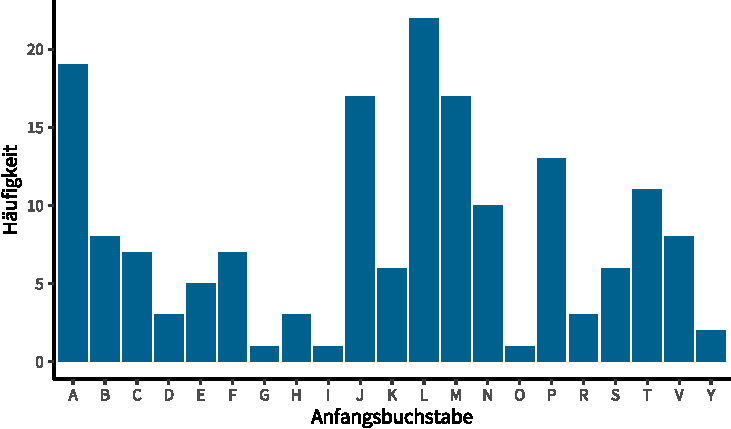
\includegraphics[width=.49\linewidth]{bookdownproj_files/figure-latex/stab-1} 

}

\caption{Stabdiagramm}\label{fig:stab}
\end{figure}

\hypertarget{quantitative-variablen-1}{%
\subsubsection{Quantitative Variablen}\label{quantitative-variablen-1}}

Das oben beschriebene Verfahren funktioniert gut für qualitative Variablen (und diskrete Variablen mit wenigen unterschiedlichen Werten). Für quantitative Variablen wird ein anderes Verfahren empfohlen.

Zur Veranschaulichung soll diese geordnete Liste von Messwerten des Stammdurchmessers von Schwarzkirschen (Beispieldatensatz \texttt{trees} aus \protect\hyperlink{ref-r}{R Core Team 2018}) dienen:

\texttt{8,3\ \ 8,6\ \ 8,8\ 10,5\ 10,7\ 10,8\ 11,0\ 11,0\ 11,1\ 11,2\ 11,3\ 11,4\ 11,4\ 11,7\ 12,0\ 12,9\ 12,9\ 13,3\ 13,7\ 13,8\ 14,0\ 14,2\ 14,5\ 16,0\ 16,3\ 17,3\ 17,5\ 17,9\ 18,0\ 18,0\ 20,6}

Für solche Verteilungen müssen zuerst Klassen (engl. \emph{bins}) gebildet werden, in denen die Werte dann zusammengefasst werden (s. Tabelle \ref{tab:haeufklass}).

\begin{table}

\caption{\label{tab:haeufklass}Häufigkeitstabelle mit klassierten Werten}
\centering
\begin{tabular}[t]{lrrrr}
\toprule
Durchmesser & Absolute Häufigkeit $f$ & $f_{kum}$ & Relative Häufigkeit & $\%_{kum}$\\
\midrule
über 8 bis 10 Zoll & 3 & 3 & 9,7\% & 9,7\%\\
über 10 bis 12 Zoll & 12 & 15 & 38,7\% & 48,4\%\\
über 12 bis 14 Zoll & 6 & 21 & 19,4\% & 67,7\%\\
über 14 bis 16 Zoll & 3 & 24 & 9,7\% & 77,4\%\\
über 16 bis 18 Zoll & 6 & 30 & 19,4\% & 96,8\%\\
über 18 bis 20 Zoll & 0 & 30 & 0\% & 96,8\%\\
über 20 bis 22 Zoll & 1 & 31 & 3,2\% & 100\%\\
\bottomrule
\end{tabular}
\end{table}

Für die Wahl der Klassengrenzen gibt es zwei feste Regeln:

\begin{itemize}
\tightlist
\item
  Alle Werte müssen abgedeckt sein.
\item
  Die Klassen dürfen sich nicht überlappen.
\end{itemize}

Zusätzlich sollten folgende Konventionen nach Möglichkeit befolgt werden:

\begin{itemize}
\tightlist
\item
  Klassen sollten gleich große Wertebereiche abdecken.
\item
  Alle Klassen sollten besetzt sein.
\item
  Klassengrenzen sollten möglichst glatte Zahlen sein.
\item
  Aus Gründen der Übersichtlichkeit sollten nicht mehr als 20 Klassen gewählt werden.
\item
  Klassengrenzen sollten ``Klumpen'' mit ähnlichen Werten nicht trennen.
\end{itemize}

Die Darstellung erfolgt in so genannten Histogrammen (engl. \emph{histogram}). Abbildung \ref{fig:hist} enthält ein Beispiel für ein Histogramm.

\begin{rtip}
In R können Histogramme mit {\tt hist()} erstellt werden.
\end{rtip}

\begin{figure}[h]

{\centering 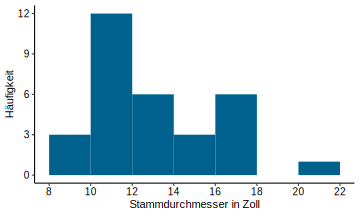
\includegraphics[width=.49\linewidth]{bookdownproj_files/figure-latex/hist-1} 

}

\caption{Histogramm}\label{fig:hist}
\end{figure}

\hypertarget{polygone}{%
\subsubsection{Polygone}\label{polygone}}

Statt ausgefüllten Flächen wie im Histogramm lassen sich für die Häufigkeiten auch Punkte setzen, die dann mit Linien verbunden werden. So entsteht ein Häufigkeitspolygon (s. Abbildung \ref{fig:poly}).

\begin{figure}[h]

{\centering 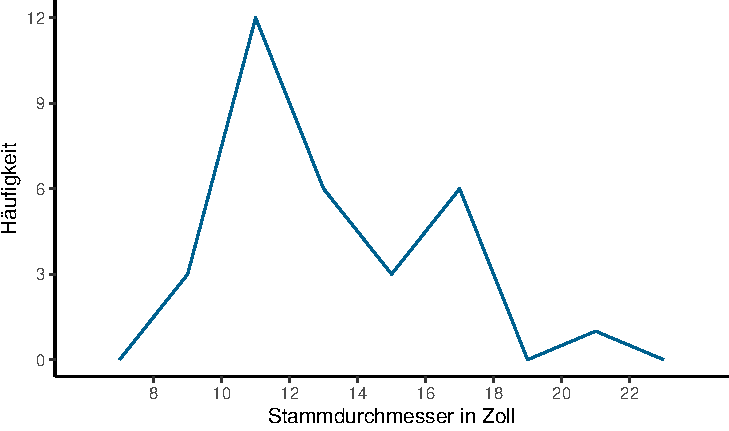
\includegraphics[width=.49\linewidth]{bookdownproj_files/figure-latex/poly-1} 

}

\caption{Polygonzug}\label{fig:poly}
\end{figure}

\hypertarget{eigenschaften-von-huxe4ufigkeitsverteilungen}{%
\subsubsection{Eigenschaften von Häufigkeitsverteilungen}\label{eigenschaften-von-huxe4ufigkeitsverteilungen}}

Polygone von Häufigkeitsverteilungen (insbesondere in geglätteter Form) ergeben Annäherungen an so gennannte Dichtefunktionen (engl. \emph{density functions}). Diese lassen sich mit Attributen (uni-/bimodal, schmal-/breitgipflig, etc.) beschreiben, wie in Abbildung 4 veranschaulicht.

\begin{figure}
\centering
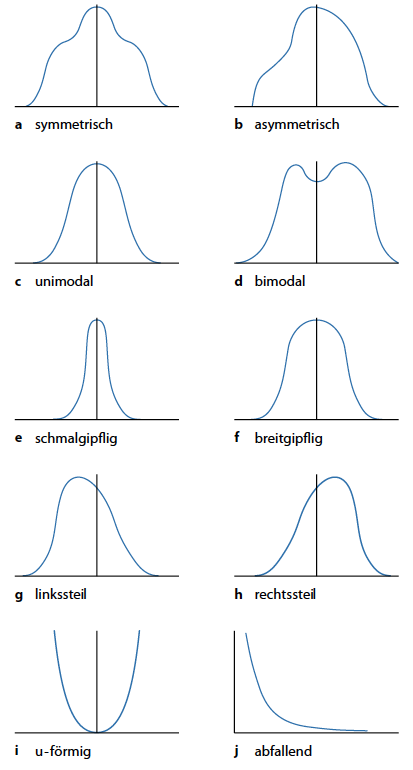
\includegraphics[width=\textwidth,height=7.29167in]{../img/shapes.png}
\caption{Merkmale von Verteilungen (aus: \protect\hyperlink{ref-bortz}{Bortz und Schuster 2010}: 42)}
\end{figure}

\pagebreak

\hypertarget{aufgaben}{%
\subsection{Aufgaben}\label{aufgaben}}

Die folgenden Aufgaben sind zur eigenständigen Überprüfung Ihrer Lernleistung gedacht (als Vor- oder Nachbereitung der Vorlesung, oder als Klausurübung) und nicht etwa als Hausaufgabe.

\hypertarget{aufgabe-1}{%
\subsubsection{Aufgabe 1}\label{aufgabe-1}}

Bestimmen Sie das Skalenniveau der folgenden Variablen. Kennzeichnen Sie darüber hinaus, ob die Variable qualitativ, diskret oder stetig ist.

\begin{enumerate}
\def\labelenumi{\alph{enumi})}
\tightlist
\item
  Lebensalter in Jahren
\item
  Regenmenge in mm
\item
  Güteklasse
\item
  Passagieraufkommen
\item
  Baujahr
\item
  Geschwindigkeit in km/h
\item
  Sozialstatus (Unter-, Mittel und Oberschicht)
\item
  Temperatur in °F
\item
  Fläche eines Bundeslands in km²
\item
  Temperatur in K
\item
  Einwohnerzahl
\item
  Pegelstand
\item
  Staatsangehörigkeit
\item
  Interesse an Statistik (gering bis hoch)
\item
  Klausurnote
\item
  Bodentyp
\item
  Entfernung zum Stadtzentrum in km
\item
  Körpergröße
\item
  Kleidergröße (S bis XXL)
\item
  Monatliches Nettoeinkommen
\end{enumerate}

\hypertarget{aufgabe-2}{%
\subsubsection{Aufgabe 2}\label{aufgabe-2}}

Folgende Werte seien erfasst über die Lebensdauer von Klimaanlagen in Stunden (Beispieldatensatz \texttt{aircondit7} aus \protect\hyperlink{ref-r}{R Core Team 2018}):\\
\texttt{14\ 23\ 15\ 139\ 13\ 39\ 188\ 22\ 50\ 3\ 36\ 46\ 30\ 5\ 102\ 5\ 88\ 22\ 197\ 72\ 210\ 97\ 79\ 44}

\begin{enumerate}
\def\labelenumi{\alph{enumi})}
\tightlist
\item
  Erstellen Sie eine Häufigkeitstabelle. Welche Klassen wählen Sie und warum?
\item
  Zeichnen Sie ein Histogramm.
\item
  Beschreiben Sie die Verteilung.
\end{enumerate}

\hypertarget{tipps-zur-vertiefung}{%
\subsection{Tipps zur Vertiefung}\label{tipps-zur-vertiefung}}

\hypertarget{grundbegriffe}{%
\subsubsection{Grundbegriffe}\label{grundbegriffe}}

\begin{itemize}
\tightlist
\item
  YouTube-Kanal ``Kurzes Tutorium Statistik'': \href{https://www.youtube.com/watch?v=bJsBcLjke3Q}{Statistische Grundbegriffe}
\item
  Kapitel 1.1 in \protect\hyperlink{ref-bortz}{Bortz und Schuster} (\protect\hyperlink{ref-bortz}{2010})
\item
  Kapitel 1.1 in \protect\hyperlink{ref-benninghaus}{Benninghaus} (\protect\hyperlink{ref-benninghaus}{2007})
\item
  Kapitel 2.1 in \protect\hyperlink{ref-bahrenberg}{Bahrenberg, Giese und Nipper} (\protect\hyperlink{ref-bahrenberg}{2010})
\end{itemize}

\hypertarget{stichproben}{%
\subsubsection{Stichproben}\label{stichproben}}

\begin{itemize}
\tightlist
\item
  Kapitel 6.1 in \protect\hyperlink{ref-bortz}{Bortz und Schuster} (\protect\hyperlink{ref-bortz}{2010})
\item
  Kapitel 2.3 in \protect\hyperlink{ref-bahrenberg}{Bahrenberg, Giese und Nipper} (\protect\hyperlink{ref-bahrenberg}{2010})
\end{itemize}

\hypertarget{skalenniveaus-1}{%
\subsubsection{Skalenniveaus}\label{skalenniveaus-1}}

\begin{itemize}
\tightlist
\item
  Kapitel 1.2 in \protect\hyperlink{ref-bortz}{Bortz und Schuster} (\protect\hyperlink{ref-bortz}{2010})
\item
  Kapitel 2.1 in \protect\hyperlink{ref-benninghaus}{Benninghaus} (\protect\hyperlink{ref-benninghaus}{2007})
\item
  Kapitel 2.2 in \protect\hyperlink{ref-bahrenberg}{Bahrenberg, Giese und Nipper} (\protect\hyperlink{ref-bahrenberg}{2010})
\item
  YouTube-Kanal ``Kurzes Tutorium Statistik'': \href{https://www.youtube.com/watch?v=TV4tTtW4UBU}{Skalenniveaus}
\end{itemize}

\hypertarget{huxe4ufigkeiten-und-diagramme}{%
\subsubsection{Häufigkeiten und Diagramme}\label{huxe4ufigkeiten-und-diagramme}}

\begin{itemize}
\tightlist
\item
  YouTube-Kanal ``Kurzes Tutorium Statistik'': \href{https://www.youtube.com/watch?v=LkOBRWXnTRQ}{Stabdiagramme und Histogramme}
\item
  Kapitel 3.1 und 3.2 in \protect\hyperlink{ref-bortz}{Bortz und Schuster} (\protect\hyperlink{ref-bortz}{2010})
\item
  Kapitel 1.2 in \protect\hyperlink{ref-benninghaus}{Benninghaus} (\protect\hyperlink{ref-benninghaus}{2007})
\item
  Kapitel 4.1 in \protect\hyperlink{ref-bahrenberg}{Bahrenberg, Giese und Nipper} (\protect\hyperlink{ref-bahrenberg}{2010})
\end{itemize}

\hypertarget{quellen}{%
\subsection{Quellen}\label{quellen}}

\hypertarget{mauxdfzahlen}{%
\section{Maßzahlen}\label{mauxdfzahlen}}

\hypertarget{lernziele-dieser-sitzung-1}{%
\subsection{Lernziele dieser Sitzung}\label{lernziele-dieser-sitzung-1}}

Sie können\ldots{}

\begin{itemize}
\tightlist
\item
  die wichtigsten Lagemaße von Stichproben bestimmen.
\item
  die wichtigsten Streumaße von Stichproben bestimmen.
\item
  Boxplots interpretieren.
\end{itemize}

\hypertarget{einleitende-bemerkungen}{%
\subsection{Einleitende Bemerkungen}\label{einleitende-bemerkungen}}

Die im Folgenden besprochenen Maßzahlen (oder Kennzahlen, Parameter) verdichten (oder aggregieren) Häufigkeitsverteilungen einer Variable. Durch diese Parameter kann das Charakteristische einer Verteilung schnell erfasst und vergleichbar gemacht werden. Die Verdichtung auf Maßzahlen geht jedoch immer auch mit Informationsverlust einher.

Die Möglichkeit der Angabe statistischer Maßzahlen ist abhängig vom Skalenniveau der Daten, wie der Überblick in Tabelle \ref{tab:mass} zeigt.

\begin{table}[!h]

\caption{\label{tab:mass}Die wichtigsten Maßzahlen}
\centering
\begin{tabular}[t]{llll}
\toprule
Parameter & Typ & Mindestes Skalenniveau & Formel\\
\midrule
Modalwert & Lagemaß & nominal & \medskip$\mathit{Mo}$\\
Median & Lagemaß & ordinal & \medskip$\def\arraystretch{1.2} \mathit{Md} = \Bigg\{\begin{array}{@{}c@{}}\frac{x_{(\frac{n}{2})}+x_{(\frac{n}{2}+1)}}{2} \quad \textrm{falls }n \textrm{ gerade}\\[6pt] x_{(\frac{n+1}{2})}\quad \textrm{falls }n \textrm{ ungerade}\end{array}$\\
Arithmetisches Mittel & Lagemaß & metrisch & \medskip$\bar{x}=\frac{\sum\limits_{i=1}^{n}x _{i}}{n}$\\
Spannweite & Streumaß & ordinal & \medskip$R=x_{(n)}-x_{(1)}$\\
Quartilsabstand & Streumaß & ordinal & \medskip$\mathit{IQR}=Q_3-Q_1$\\
\addlinespace
Varianz & Streumaß & metrisch & \medskip$s^2=\frac{\sum\limits_{i=1}^{n}(x_{i}-\bar{x})^2}{n-1}$\\
Standardabweichung & Streumaß & metrisch & \medskip$s=\sqrt{s^2}$\\
\bottomrule
\end{tabular}
\end{table}

\hypertarget{beispielverteilung}{%
\subsubsection{Beispielverteilung}\label{beispielverteilung}}

Alle Berechnungen von Maßzahlen werden am folgenden Beispiel illustriert: Für die 14 Gemeinden im Landkreis Rothenberge wurde die jeweilige Anzahl an Gaststätten erhoben. Die Zählung ergab die Wertereihe in Tabelle \ref{tab:werte}.

\begin{table}[!h]

\caption{\label{tab:werte}Beispielverteilung}
\centering
\begin{tabular}[t]{rrrrrrrrrrrrrr}
\toprule
$x_{1}$ & $x_{2}$ & $x_{3}$ & $x_{4}$ & $x_{5}$ & $x_{6}$ & $x_{7}$ & $x_{8}$ & $x_{9}$ & $x_{10}$ & $x_{11}$ & $x_{12}$ & $x_{13}$ & $x_{14}$\\
\midrule
4 & 1 & 4 & 1 & 5 & 5 & 0 & 1 & 8 & 5 & 1 & 25 & 3 & 3\\
\bottomrule
\end{tabular}
\end{table}

\hypertarget{lagemauxdfe}{%
\subsection{Lagemaße}\label{lagemauxdfe}}

Lagemaße (auch Maße der Zentraltendenz, Lokalisationsparameter, Mittelwerte, engl. \emph{measures of central tendency}) bezeichnen alle statistischen Maßzahlen, die eine Verteilung repräsentieren, indem sie die Lage der mittleren oder häufigsten Variablenwerte angeben.

Im Falle einer unimodalen, perfekt symmetrischen Verteilung (z.B. Glockenform) haben alle drei Lageparameter den gleichen Wert. Je weiter Verteilungen von dieser Form abweichen -- durch Mehrgipfligkeit oder Asymmetrie -- desto unpräziser ist die Beschreibung der Verteilung durch einen einzigen Parameter.

\hypertarget{median}{%
\subsubsection{Median}\label{median}}

Der Median (engl. \emph{median}) einer Verteilung ist der Wert, der größer als genau 50\% aller Werte ist.

Da dies eine Größer-kleiner-Relation der Werte voraussetzt, kann der Median nur für ordinale und metrische Skalenniveaus angegeben werden.

Im Folgenden wird die (einfachere) Bestimmung des Medians nach \protect\hyperlink{ref-bortz}{Bortz und Schuster} (\protect\hyperlink{ref-bortz}{2010}) verwendet. \protect\hyperlink{ref-benninghaus}{Benninghaus} (\protect\hyperlink{ref-benninghaus}{2007}) beschreibt ein anderes Verfahren, welches zu anderen Ergebnissen kommen kann.

Um den Median zu bestimmen, wird zunächst eine geordnete Liste angefertigt, indem die Werte aufsteigend sortiert werden. Diese sortierten Werte werden mit \(x_{(1)}, x_{(2)}, x_{(3)}, ..., x_{(n)}\) bezeichnet (also mit Klammern). Für unsere Beispielverteilung ergibt sich Tabelle \ref{tab:sort}.

\begin{table}[!h]

\caption{\label{tab:sort}Sortierte Wertereihe}
\centering
\begin{tabular}[t]{rrrrrrrrrrrrrr}
\toprule
$x_{(1)}$ & $x_{(2)}$ & $x_{(3)}$ & $x_{(4)}$ & $x_{(5)}$ & $x_{(6)}$ & $x_{(7)}$ & $x_{(8)}$ & $x_{(9)}$ & $x_{(10)}$ & $x_{(11)}$ & $x_{(12)}$ & $x_{(13)}$ & $x_{(14)}$\\
\midrule
0 & 1 & 1 & 1 & 1 & 3 & 3 & 4 & 4 & 5 & 5 & 5 & 8 & 25\\
\bottomrule
\end{tabular}
\end{table}

Bei einer ungeraden Stichprobengröße \(n\) teilt der \((\frac{n+1}{2})\)-te Wert (also der Wert genau in der Mitte) die Stichprobe in zwei Hälften, weshalb gilt:

\[
  \mathit{Md} = x_{(\frac{n+1}{2})} \quad \text{falls }n\text{ ungerade.}
\]\{\#eq:med1\}

Bei geradem \(n\) entstehen zwei gleich große Hälften der Stichprobe: \(x_{(1)}\) bis \(x_{(\frac{n}{2})}\) einerseits, und \(x_{(\frac{n}{2}+1)}\) bis \(x_{(n)}\) andererseits. Der Durchschnitt zwischen \(x_{(\frac{n}{2})}\) und \(x_{(\frac{n}{2}+1)}\) teilt die Stichprobe in zwei Hälften. Es gilt:

\[
  \mathit{Md} = \frac{x_{(\frac{n}{2})} + x_{(\frac{n}{2}+1)}}{2} \quad \text{falls } n \text{ gerade.}
\]\{\#eq:med2\}

In unserem Beispiel ist \(n=14\) und damit gerade. Der Median errechnet also nach Formel \ref{eq:med2} wie folgt:

\[
  \begin{aligned}
    \mathit{Md} & = \frac{x_{(7)} + x_{(8)}}{2} \\[4pt]
                & = \frac{3 + 4}{2} \\[4pt]
                & = 3,5
  \end{aligned}
\]

\begin{rtip}
In R gibt die Funktion {\tt median()} den Median einer Verteilung aus.
\end{rtip}

\hypertarget{modalwert}{%
\subsubsection{Modalwert}\label{modalwert}}

Der Modalwert \(\mathit{Mo}\) (auch Modus, engl. \emph{mode}) gibt den häufigsten Wert oder die häufigsten Werte einer Verteilung an.

Der Modalwert kann so auch (als einziger Mittelwert) für nominalskalierte Variablen angegeben werden.

Bei ordinalen und metrischen Skalenniveaus sind folgende Besonderheiten zu beachten:

\begin{itemize}
\tightlist
\item
  Wird der Modus einer Verteilung durch unmittelbar benachbarte Werte gebildet, wird er als Kombination (bei metrischen Variablen als arithmetisches Mittel) dieser Werte angegeben.
\item
  Bei bimodalen (multimodalen) Verteilungen werden beide (alle) Modalwerte angegeben.
\end{itemize}

Hierzu müssen die Häufigkeiten der Werte bekannt sein, bzw. bestimmt werden (s. Tabelle \ref{tab:mod}).

\begin{table}[H]

\caption{\label{tab:mod}Häufigkeiten der Beispielverteilung}
\centering
\begin{tabular}[t]{rr}
\toprule
Wert $x_i$ & Häufigkeit $f_i$\\
\midrule
0 & 1\\
1 & 4\\
3 & 2\\
4 & 2\\
5 & 3\\
8 & 1\\
25 & 1\\
\bottomrule
\end{tabular}
\end{table}

Der Modalwert der Beispielverteilung beträgt 1, da der Wert 1 am häufigsten (viermal) vorkommt.

\hypertarget{arithmetisches-mittel}{%
\subsubsection{Arithmetisches Mittel}\label{arithmetisches-mittel}}

Das arithmetische Mittel (auch Mittelwert, Durchschnitt, engl. \emph{mean}) ist das gebräuchlichste Lagemaß und Grundlage für viele statistische Verfahren.

Das arithmetische Mittel setzt ein metrisches Skalenniveau voraus.

Die Berechnung des arithmetischen Mittels einer Stichprobe erfolgt durch die Formel:

\[
 \bar{x}=\frac{\sum\limits _{i=1}^{n}x_{i}}{n}
\]\{\#eq:am\}

Für unsere Beispielverteilung ergibt sich durch einsetzen in Formel \ref{eq:am}:
\[
  \begin{aligned}
     \bar{x}&=\frac{\sum\limits _{i=1}^{14}x_{i}}{14} \\[4pt]
            &=\frac{4+1+4+1+5+5+0+1+8+5+1+25+3+3}{14} \\[4pt]
            &=\frac{63}{14}\\[4pt]
            &\approx 4,71
  \end{aligned}
\]

\begin{rtip}
Der Befehl für die Ermittlung des arithmetischen Mittels in R lautet {\tt mean()}.
\end{rtip}

\hypertarget{streumauxdfe}{%
\subsection{Streumaße}\label{streumauxdfe}}

Streumaße (auch Streuungs-, Variabilitäts-, Dispersionswerte, engl. \emph{measures of variability}) geben Auskunft darüber, wie heterogen die Werte einer Verteilung sind, d.h. wie breit sie gestreut sind. Während Lagemaße den typischen Wert einer Verteilung ermitteln, zeigen Streumaße, wie gut (oder eigentlich: wie schlecht) dieser typische Wert die Verteilung repräsentiert.

\hypertarget{spannweite}{%
\subsubsection{Spannweite}\label{spannweite}}

Die Spannweite (engl. \emph{range}) gibt Auskunft darüber, wie groß der Wertebereich ist, der von einer Verteilung abgedeckt wird. Sie wird (für metrische Skalen) als die Differenz vom größten zum kleinsten Wert (also vom letzten zum ersten Wert einer geordneten Werteliste) angegeben:

\[
 R=x_{(n)} - x_{(1)}
\]\{\#eq:range\}

Für unsere Beispielstichprobe ergibt sich (mit Blick auf Tabelle \ref{tab:sort}):

\nopagebreak

\[
  \begin{aligned}
     R&=x_{(14)} - x_{(1)} \\[4pt]
     &=25-0 \\[4pt]
     &=25
  \end{aligned}
\]

\begin{rtip}
In R gibt die Funktion {\tt range()} die Werte für $x_{(1)}$ und $x_{(n)}$ aus.
\end{rtip}

\hypertarget{quartilsabstand}{%
\subsubsection{Quartilsabstand}\label{quartilsabstand}}

Der Quartilsabstand (auch Interquartilsabstand, engl. \emph{interquartile range / IQR}) gibt die Größe des Wertebereichs der mittleren 50\% einer Verteilung an.

Genau so wie der Median eine Messwertreihe in zwei gleich große Hälften ``schneidet'', schneiden die Quartile die Werte in Viertel. Dabei liegt der so genannte untere Angelpunkt \(Q_1\) genau über 25\% der Werte, \(Q_2\) ist identisch mit dem Median und der obere Angelpunkt \(Q_3\) liegt genau über 75\% der Werte.

Der Angelpunkt \(Q_1\) wird ermittelt, indem der Median für die unteren 50\% (\(Q_3\): die oberen 50\%) der Werte bestimmt wird -- also jener Werte, die theoretisch unterhalb des Medians der Gesamtverteilung liegen.

Dabei folgen wir \protect\hyperlink{ref-bortz}{Bortz und Schuster} (\protect\hyperlink{ref-bortz}{2010}) und nehmen im Fall eines ungeraden \(n\) den Median auf beiden Seiten hinzu.

Die Formel für den Quartilsabstand lautet:

\[
  \begin{aligned}
    \mathit{IQR}=Q_3-Q_1
  \end{aligned}
\]\{\#eq:iqr\}

Der Quartilsabstand ist Ausreißern gegenüber stabiler als die Spannweite, da extreme hohe oder niedrige Wert nicht in die Berechnung einfließen.

In unserem Beispiel (mit \(n=14\)) ist die untere Hälfte der Verteilung:

\begin{table}[H]
\centering
\begin{tabular}{rrrrrrr}
\toprule
$x_{(1)}$ & $x_{(2)}$ & $x_{(3)}$ & $x_{(4)}$ & $x_{(5)}$ & $x_{(6)}$ & $x_{(7)}$\\
\midrule
0 & 1 & 1 & 1 & 1 & 3 & 3\\
\bottomrule
\end{tabular}
\end{table}

\(Q_1\) ist der Median dieser Werte, also \(x_{(4)}=1\).

Die oberen 7 Werte lauten:

\begin{table}[H]
\centering
\begin{tabular}{rrrrrrr}
\toprule
$x_{(8)}$ & $x_{(9)}$ & $x_{(10)}$ & $x_{(11)}$ & $x_{(12)}$ & $x_{(13)}$ & $x_{(14)}$\\
\midrule
4 & 4 & 5 & 5 & 5 & 8 & 25\\
\bottomrule
\end{tabular}
\end{table}

\(Q_3\) ist also \(x_{(11)} = 5\).

Für den Quartilsabstand ergibt sich durch einsetzen in Formel \ref{eq:iqr}:

\[
  \begin{aligned}
    \mathit{IQR}&=5-1 \\[4pt]
       &=4 \\[4pt]
  \end{aligned}
\]

\begin{rtip}
In R werden die Quartile üblicherweise mit {\tt quantile()} und der Quartilsabstand mit {\tt IQR()} bestimmt.

\medskip

\textbf{Achtung:} Genau wie für den Median gibt es auch für die Ermittlung der Quartile bzw. des Quartilsabstands unterschiedliche Verfahren. Die Ergebnisse dieser R-Funktionen weichen hier deshalb meist leicht vom hier besprochenen Verfahren ab!
\end{rtip}

\hypertarget{varianz}{%
\subsubsection{Varianz}\label{varianz}}

Die Varianz einer Messwertreihe (engl. \emph{variance}) kann verstanden werden als der durschnittliche quadrierte Abstand der Werte zum arithmetischen Mittel.

Die Formel lautet:

\[s^2=\frac{\sum\limits_{i=1}^{n}(x_{i}-\bar{x})^2}{n-1}\]\{\#eq:var\}

Die Quadrierung der Differenz hat dabei einen doppelten Effekt: Zum einen bekommen auch negative Differenzen ein positives Vorzeichen, so dass sich positive und negative Differenzen nicht neutralisieren. Zum anderen werden hierdurch besonders große Abweichungen zum arithmetischen Mittel stärker gewichtet als dies ohne Quadrierung der Fall wäre.

Zudem fällt auf, dass im Gegensatz zur Formel für das arithmetische Mittel im Nenner \(n-1\) steht und nicht etwa \(n\). Dies hat mit so genannten Freiheitsgraden zu tun, die wir allerdings erst in Sitzung 6 genauer kennenlernen.

Für unsere Beispielstichprobe wird die Berechnung für alle einzelnen \((x_i-\bar{x})^2\) schnell aufwendig und unübersichtich. Deshalb berechnen wir ihre Summe hier mit Hilfe einer Häufigkeitstabelle (s. Tabelle \ref{tab:freq}). Dabei werden alle distinkten Werte einzeln transformiert und in der letzten Spalte mit ihrer Häufigkeit multipliziert.

\begin{table}

\caption{\label{tab:freq}Häufigkeitstabelle zur Berechnung der Varianz}
\centering
\begin{tabular}[t]{rrrrr}
\toprule
\multicolumn{1}{c}{Wert} & \multicolumn{1}{c}{Häufigkeit} & \multicolumn{1}{c}{Abweichung vom Mittel} & \multicolumn{1}{c}{Quadrat der Abweichung} & \multicolumn{1}{c}{Produkt mit Häufigkeit} \\
\cmidrule(l{3pt}r{3pt}){1-1} \cmidrule(l{3pt}r{3pt}){2-2} \cmidrule(l{3pt}r{3pt}){3-3} \cmidrule(l{3pt}r{3pt}){4-4} \cmidrule(l{3pt}r{3pt}){5-5}
$x_i$ & $f_i$ & $(x_i- \bar{x})$ & $(x_i- \bar{x})^2$ & $f_i\cdot(x_i -\bar{x})^2$\\
\midrule
0 & 1 & -4,71 & 22,18 & 22,18\\
1 & 4 & -3,71 & 13,76 & 55,04\\
3 & 2 & -1,71 & 2,92 & 5,84\\
4 & 2 & -0,71 & 0,50 & 1,00\\
5 & 3 & 0,29 & 0,08 & 0,24\\
8 & 1 & 3,29 & 10,82 & 10,82\\
25 & 1 & 20,29 & 411,68 & 411,68\\
\bottomrule
\end{tabular}
\end{table}

Schließlich werden die Werte in Formel \ref{eq:var} eingesetzt:

\nopagebreak

\[\begin{aligned}
    s^2&=\frac{\sum\limits_{i=1}^{14}(x_{i}-\bar{x})^2}{14-1} \\[4pt]
       &\approx\frac{22,18+55,04+5,84+1+0,24+10,82+411,68}{13} \\[4pt]
       &=\frac{506,80}{13}\\[4pt]
       &\approx 38,98
\end{aligned}\]

Eine solche Tabelle lässt sich analog auch für die Berechnung von Summen größerer Messwertreihen für das arithmetische Mittel verwenden.

Zudem lässt dieses Verfahren sich auf klassierte Daten anwenden, wenn für \(x_i\) der Mittelwert der Klassen eingesetzt wird (womit allerdings Informations- und Präzisionsverlust einhergeht).

\begin{rtip}
In R lautet der Befehl für die Errechnung der Varianz {\tt var()}.
\end{rtip}

\hypertarget{standardabweichung}{%
\subsubsection{Standardabweichung}\label{standardabweichung}}

Die Standardabweichung (engl. \emph{standard deviation}) ist das gebräuchlichste Streumaß und spielt eine herausragende Rolle in den allermeisten statistischen Verfahren.

Die Standardabweichung einer Messwertreihe ist definiert als die Quadraturzel ihrer Varianz:

\[
  \begin{aligned}
    s=\sqrt{s^2}
  \end{aligned}
\]\{\#eq:sd\}

Indem hier die Wurzel gezogen wird, wird in gewisser Weise die Quadrierung der Differenzen für die Varianz wieder ``korrigiert''. Insbesondere wird die Quadrierung der Maßeinheit wieder aufgehoben -- die Standardabweichung hat also die gleiche Einheit wie die Messreihe selbst.

In unserem Beispiel beträgt die Standardabweichung also:

\[
  \begin{aligned}
    s&\approx\sqrt{38,98}
      \approx6,24
  \end{aligned}
\]

\begin{rtip}
Die Standardabweichung wird in R mit der Funktion {\tt sd()} berechnet.
\end{rtip}

\hypertarget{boxplot}{%
\subsection{Boxplot}\label{boxplot}}

Der Boxplot (auch Box-and-whisker-plot) kombiniert einige der gebräuchlichsten Maßzahlen in einer übersichtlichen Grafik (s. Abbildung \ref{fig:box}).

\begin{figure}[h]

{\centering 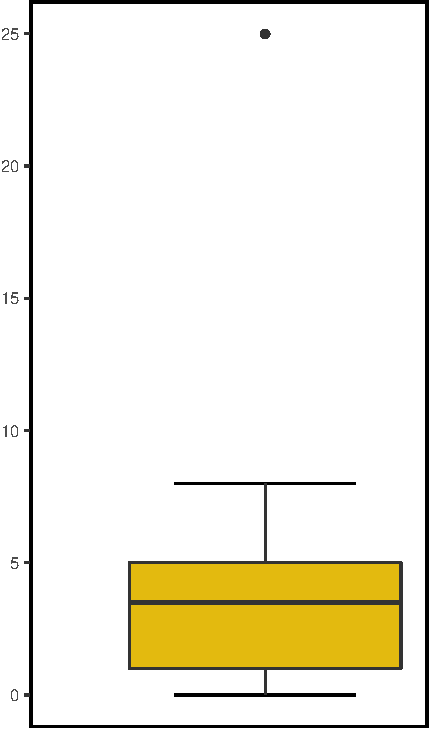
\includegraphics[width=.3\linewidth]{bookdownproj_files/figure-latex/box-1} 

}

\caption{Boxplot der Beispielverteilung}\label{fig:box}
\end{figure}

Die Höhe der ``Box'' definiert sich durch den Quartilsabstand, der mittlere Strich markiert den Median und die ``Whisker'' markieren den Wertebereich insgesamt -- wobei Ausreißer, deren Abstand zur Box mehr als das 1,5-Fache des Quartilsabstands beträgt, üblicherweise gar nicht oder (wie hier) gesondert mit Punkten markiert werden.

\begin{rtip}
In R lässt sich ein Boxplot mit dem Befehl {\tt boxplot()} ausgeben.
\end{rtip}

\hypertarget{aufgaben-1}{%
\subsection{Aufgaben}\label{aufgaben-1}}

Die folgenden Aufgaben sind zur eigenständigen Überprüfung Ihrer Lernleistung gedacht (als Vor- oder Nachbereitung der Vorlesung, oder als Klausurübung) und nicht etwa als Hausaufgabe.

\hypertarget{aufgabe-1-1}{%
\subsubsection{Aufgabe 1}\label{aufgabe-1-1}}

Bei einer Befragung jedes 500. Studierenden im Matrikel einer privaten Hochschule wurden folgende Angaben zur Haushaltsgröße gemacht:

\texttt{1\ 4\ 4\ 2\ 3\ 2\ 3\ 5\ 2\ 7\ 2\ 1\ 1}

\begin{enumerate}
\def\labelenumi{\alph{enumi})}
\tightlist
\item
  Welches Skalenniveau liegt vor? (Sitzung 1)
\item
  Berechnen Sie Modalwert,
\item
  Median und
\item
  arithmetisches Mittel der Stichprobe.
\item
  Berechnen Sie außerdem die Spannweite,
\item
  den Quartilsabstand,
\item
  die Varianz und
\item
  die Standardabweichung der Stichprobe.
\item
  Zeichnen Sie einen Boxplot der Stichprobenverteilung.
\end{enumerate}

\hypertarget{aufgabe-2-1}{%
\subsubsection{Aufgabe 2}\label{aufgabe-2-1}}

In Australien betrug die durchnittliche Niederschlagsmenge in den 1970er und 80er Jahren:\footnote{Auszug aus dem Datensatz \texttt{bomsoi} in (\protect\hyperlink{ref-daag}{\textbf{daag?}})}
\nopagebreak

\begin{table}
\centering\begingroup\fontsize{8}{10}\selectfont

\begin{tabular}{rr}
\toprule
Jahr & Niederschlag (mm)\\
\midrule
1970 & 384,52\\
1971 & 493,65\\
1972 & 364,65\\
1973 & 661,32\\
1974 & 785,27\\
1975 & 603,45\\
1976 & 527,75\\
1977 & 471,81\\
1978 & 525,65\\
1979 & 455,64\\
1980 & 433,01\\
1981 & 535,12\\
1982 & 421,36\\
1983 & 499,29\\
1984 & 555,21\\
1985 & 398,88\\
1986 & 391,96\\
1987 & 453,41\\
1988 & 459,84\\
1989 & 483,78\\
\bottomrule
\end{tabular}
\endgroup{}
\end{table}

\begin{enumerate}
\def\labelenumi{\alph{enumi})}
\tightlist
\item
  Welches Skalenniveau liegt vor? (Sitzung 1)
\item
  Legen Sie eine klassierte Häufigkeitstabelle an. Begründen Sie die Wahl der Klassen. (Sitzung 1)
\item
  Was ist der Modalwert der klassierten Verteilung?
\item
  Wie groß ist der Quartilsabstand?
\item
  Bestimmen Sie das arithmetische Mittel der klassierten Verteilung.
\item
  Berechnen Sie die Standardabweichung.
\item
  Zeichnen Sie einen Boxplot für die Verteilung.
\end{enumerate}

\hypertarget{tipps-zur-vertiefung-1}{%
\subsection{Tipps zur Vertiefung}\label{tipps-zur-vertiefung-1}}

\hypertarget{lagemauxdfe-1}{%
\subsubsection{Lagemaße}\label{lagemauxdfe-1}}

\begin{itemize}
\tightlist
\item
  Kapitel 3.3.1 in \protect\hyperlink{ref-benninghaus}{Benninghaus} (\protect\hyperlink{ref-benninghaus}{2007})
\item
  Kapitel 2.1 in \protect\hyperlink{ref-bortz}{Bortz und Schuster} (\protect\hyperlink{ref-bortz}{2010})
\item
  Kapitel 4.2.1 in \protect\hyperlink{ref-bahrenberg}{Bahrenberg, Giese und Nipper} (\protect\hyperlink{ref-bahrenberg}{2010})
\item
  YouTube-Kanal ``Kurzes Tutorium Statistik'': \href{https://www.youtube.com/watch?v=Kx9aHOMVPEg}{Arithmetisches, harmonisches und geometrisches Mittel}
\item
  YouTube-Kanal ``Kurzes Tutorium Statistik'': \href{https://www.youtube.com/watch?v=HsDeAoBOyS4}{Boxplots, Median, Quartile}
\end{itemize}

\hypertarget{streumauxdfe-1}{%
\subsubsection{Streumaße}\label{streumauxdfe-1}}

\begin{itemize}
\tightlist
\item
  Kapitel 3.1.2 in \protect\hyperlink{ref-benninghaus}{Benninghaus} (\protect\hyperlink{ref-benninghaus}{2007})
\item
  Kapitel 2.2 in \protect\hyperlink{ref-bortz}{Bortz und Schuster} (\protect\hyperlink{ref-bortz}{2010})
\item
  Kapitel 4.2.2 in \protect\hyperlink{ref-bahrenberg}{Bahrenberg, Giese und Nipper} (\protect\hyperlink{ref-bahrenberg}{2010})
\item
  YouTube-Kanal ``Kurzes Tutorium Statistik'': \href{https://www.youtube.com/watch?v=3oZrS3ZWVcA}{Streumaße - Varianz, Standardabweichung, Variationskoeffizient und mehr!}
\end{itemize}

\hypertarget{boxplot-1}{%
\subsubsection{Boxplot}\label{boxplot-1}}

\begin{itemize}
\tightlist
\item
  Kapitel 3.4 in \protect\hyperlink{ref-bortz}{Bortz und Schuster} (\protect\hyperlink{ref-bortz}{2010})
\item
  YouTube-Kanal ``Kurzes Tutorium Statistik'': \href{https://www.youtube.com/watch?v=HsDeAoBOyS4}{Boxplots, Median, Quartile}
\end{itemize}

\hypertarget{quellen-1}{%
\subsection{Quellen}\label{quellen-1}}

\hypertarget{z-werte-und-normalverteilung}{%
\section{z-Werte und Normalverteilung}\label{z-werte-und-normalverteilung}}

\hypertarget{lernziele-dieser-sitzung-2}{%
\subsection{Lernziele dieser Sitzung}\label{lernziele-dieser-sitzung-2}}

Sie können\ldots{}

\begin{itemize}
\tightlist
\item
  z-Werte ermitteln.
\item
  Merkmale der Normalverteilung wiedergeben.
\item
  anhand einer normalverteilten Dichtefunktion\ldots{}

  \begin{itemize}
  \tightlist
  \item
    Wahrscheinlichkeiten errechnen.
  \item
    Perzentile errechnen.
  \end{itemize}
\end{itemize}

\hypertarget{variationskoeffizient}{%
\subsection{Variationskoeffizient}\label{variationskoeffizient}}

Die Berechnung von Maßzahlen (Sitzung 2) vereinfacht es uns, auch große Verteilungen miteinander zu vergleichen. Voraussetzung dafür ist jedoch, dass die Kennwerte (wie arithmetisches Mittel, Standardabweichung) in derselben Maßeinheit (kg, cm, °C, etc.) vorliegen und einen vergleichbaren Maßstab haben.

Eine Möglichkeit, unabhängig hiervon eine Aussage über die \emph{relative} Streuung zu treffen, ist der Variationskoeffizient (engl. \emph{coefficient of variation}) \(v\). Er ist definiert als das (prozentuale) Verhältnis von Standardabweichung zu Mittelwert:

\[\begin{aligned}
v=\frac{s}{|\bar{x}|}\cdot 100\%
\end{aligned}
\]\{\#eq:cv\}

Zur Illustration: An zufälligen Tagen hat die Wetterstation auf dem Feldberg folgende Luftdruckwerte gemessen (in hPa):

\texttt{1007,1\ 1003,4\ \ 990,7\ \ 994,2\ 1000,9\ \ 993,0\ 1016,0\ \ 983,9\ 1007,4\ \ 997,8\ \ 997,9\ 1000,2}

Mit den bekannten Methoden (Sitzung 2) können wir das arithmetische Mittel \(\bar{x}\approx 999,37\) und die Standardabweichung \(s\approx8,56\) der Stichprobe bestimmen. Durch einsetzen dieser Werte in \autoref{eq:cv} ergibt sich:

\[\begin{aligned}
v&\approx\frac{8,56}{999,37}\cdot 100\%\\[4pt]
 &\approx0,86\%
\end{aligned}
\]

Da die Standardabweichung im Vergleich zu den absoluten Werten sehr klein ist, ist der Variationskoeffizient hier sehr klein.

Ein Problem ergibt sich, wenn der Mittelwert einer Verteilung nahe Null liegt (z.B. wenn die Reihe auch negative Messwerte enthält). Der Variationskoeffizient wird in diesem Fall sehr groß und verliert stark an Aussagekraft.

\hypertarget{z-transformation}{%
\subsection{\texorpdfstring{\(z\)-Transformation}{z-Transformation}}\label{z-transformation}}

Ein weiterer Ansatz, Verteilungsmuster vergleichbar zu machen, ist die \(z\)-Transformation (auch Standardisierung, engl. \emph{standardization}).

Für jeden der Messwerte lässt sich ein entsprechender \(z\)-Wert mit dieser Formel errechnen:

\[
z=\frac{x-\bar{x}}{s}
\]\{\#eq:z\}

Der \(z\)-Wert eines Werts \(x\) ist also der Abstand des Werts zum arithmetischen Mittel \(\bar{x}\) der Verteilung, ausgedrückt im Verhältnis zu ihrer Standardabweichung \(s\).

Die einzelnen \(z\)-Werte für die Luftdruckmessungen ergeben sich wie in \autoref{tab:trans} dargestellt.

\begin{table}

\caption{\label{tab:trans}$z$-Transformation}
\centering
\begin{tabular}[t]{rcr}
\toprule
$x_i$ & Berechnung & $z_i$\\
\midrule
1007,1 & $z_{1}=\frac{1007,1-999,37}{8,56}$\medskip & 0,90\\
1003,4 & $z_{2}=\frac{1003,4-999,37}{8,56}$\medskip & 0,47\\
990,7 & $z_{3}=\frac{990,7-999,37}{8,56}$\medskip & -1,01\\
994,2 & $z_{4}=\frac{994,2-999,37}{8,56}$\medskip & -0,60\\
1000,9 & $z_{5}=\frac{1000,9-999,37}{8,56}$\medskip & 0,18\\
\addlinespace
993,0 & $z_{6}=\frac{993-999,37}{8,56}$\medskip & -0,74\\
1016,0 & $z_{7}=\frac{1016-999,37}{8,56}$\medskip & 1,94\\
983,9 & $z_{8}=\frac{983,9-999,37}{8,56}$\medskip & -1,81\\
1007,4 & $z_{9}=\frac{1007,4-999,37}{8,56}$\medskip & 0,94\\
997,8 & $z_{10}=\frac{997,8-999,37}{8,56}$\medskip & -0,18\\
\addlinespace
997,9 & $z_{11}=\frac{997,9-999,37}{8,56}$\medskip & -0,17\\
1000,2 & $z_{12}=\frac{1000,2-999,37}{8,56}$\medskip & 0,10\\
\bottomrule
\end{tabular}
\end{table}

Eine so \(z\)-transformierte Verteilung hat \emph{immer} automatisch das arithmetische Mittel \(\bar{z}=0\) und die Standardabweichung \(s_z=1\). Außerdem haben \(z\)-Werte keine Maßeinheit. So kann jede Verteilung ``standardisiert'' und systematisch vergleichbar gemacht werden.

\begin{rtip}
In R kann eine empirische Verteilung mit dem Behfehl {\tt scale()} $z$-transformiert werden.
\end{rtip}

Andersherum lassen sich \(z\)-Werte folgendermaßen wieder umwandeln in \(x\)-Werte:

\[
  x=s\cdot z+\bar{x}
\]\{\#eq:zrev\}

\hypertarget{normalverteilung}{%
\subsection{Normalverteilung}\label{normalverteilung}}

\begin{figure}[b]

{\centering 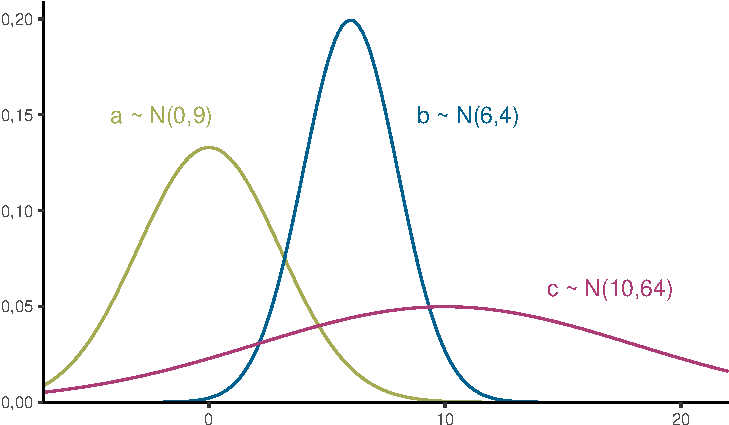
\includegraphics[width=.49\linewidth]{bookdownproj_files/figure-latex/norms-1} 

}

\caption{Dichtefunktionen verschiedener Normalverteilungen}\label{fig:norms}
\end{figure}

Die Normalverteilung (auch: Gaußverteilung, engl. \emph{normal distribution}) ist unimodal und symmetrisch. Die Normalverteilung ist eine theoretische Verteilung, für die bekannt ist, mit welcher Wahrscheinlichkeit bestimmte Werte unter- und überschritten werden bzw. mit welcher Wahrscheinlichkeit Werte in einem bestimmten Intervall liegen.

Die Dichtefunktion einer Normalverteilung hat eine markante Glockenform (s. Abbildungen \ref{fig:norms} und \ref{fig:stdnorm}). Die beiden Wendepunkte einer Normalverteilung (also dort, wo die Steigung zwischen zu- und abnehmend wechselt; oder mathematisch: wo die Ableitung der Dichtefunktion einen Extremwert annimmt) sind je eine Standardabweichung vom Mittelwert entfernt.

Die Dichtefunktion nimmt nie den Wert Null an -- Extremwerte sind also sehr selten bzw. unwahrscheinlich, aber nie unmöglich. Perfekte Normalverteilungen kommen in empirischen Beobachtungen nicht vor, sondern nur Annäherungen.

Da es sich um eine \emph{theoretische} Verteilung handelt, ist die Normalverteilung zunächst insbesondere in Bezug auf die Grundgesamtheit interessant. Im Kontext der Grundgesamtheit wird das arithmetische Mittel mit \(\mu\) (``Mü'') und die Standardabweichung mit \(\sigma\) (``Sigma'') bezeichnet (s. \autoref{tab:param}).

\begin{table}[H]

\caption{\label{tab:param}Bezeichnung von Parametern in Stichprobe und Grundgesamtheit}
\centering
\begin{tabular}[t]{lll}
\toprule
Parameter & Stichprobe & Grundgesamtheit\\
\midrule
Anzahl Elemente & $n$ & $N$\\
Arithmetisches Mittel & $\bar{x}$ & $\mu$\\
Varianz & $s^2$ & $\sigma^2$\\
Standardabweichung & $s$ & $\sigma$\\
\bottomrule
\end{tabular}
\end{table}

Jede Normalverteilung lässt sich anhand von zwei Parametern beschreiben: ihr arithmetisches Mittel und ihre Standardabweichung. Normalverteilte Grundgesamtheiten werden so notiert:

\nopagebreak

\[\begin{aligned}
x \sim N(\mu,\enspace\sigma^2)
\end{aligned}\]\{\#eq:norm\}

Der Mittelwert \(\mu\) bestimmt die Lage der Kurve auf der x-Achse, die Varianz \(\sigma^2\) bestimmt die ``Stauchung'' der Kurve (je größer desto flacher). Es gibt also unendlich viele verschiedene Normalverteilungen (s. \autoref{fig:norms}).

\hypertarget{standardnormalverteilung}{%
\subsection{Standardnormalverteilung}\label{standardnormalverteilung}}

Die Standardnormalverteilung (engl. \emph{standard normal distribution}) ist sozusagen das Grundmuster aller Normalverteilungen. Sie hat den Mittelwert \(\mu=0\) und die Standardabweichung \(\sigma=1\) (s. \autoref{fig:stdnorm}).

Alle Normalverteilungen lassen sich durch die \(z\)-Transformation auf die Standardnormalverteilung standardisieren.

\begin{figure}[h]

{\centering 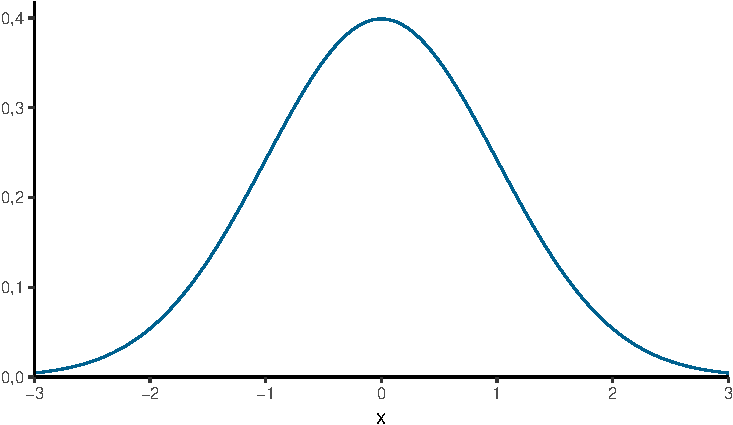
\includegraphics[width=.49\linewidth]{bookdownproj_files/figure-latex/stdnorm-1} 

}

\caption{Dichtefunktion der Standardnormalverteilung}\label{fig:stdnorm}
\end{figure}

\hypertarget{crash-kurs-wahrscheinlichkeitsrechnung}{%
\subsection{Crash-Kurs Wahrscheinlichkeitsrechnung}\label{crash-kurs-wahrscheinlichkeitsrechnung}}

Ein Zufallsexperiment ist ein beliebig oft wiederholbarer, nach bestimmten Vorschriften ausgeführter Versuch, dessen Ergebnis zufallsbedingt ist (d.~h. nicht eindeutig voraussagbar ist).

Jedem zufälligen Ereignis \(A\) ist eine bestimmte ``Wahrscheinlichkeit des Auftretens'' (engl. \emph{probability}) \(P(A)\) zugeordnet, die der Ungleichung \(0 \leq P(A) \leq 1\) genügt (d.~h. zwischen 0 und 1 liegt).

Die Wahrscheinlichkeit eines sicheren Ergebnisses A ist \(P(A) = 1\). Hingegen würde \(P(B) = 0\) bedeuten, dass das Ereignis B nicht eintreten kann. Die Summe der Wahrscheinlichkeiten aller möglichen Ereignisse beträgt 1.

Der \emph{Additionssatz} besagt: Die Wahrscheinlichkeit, dass eins von verschiedenen zufälligen, sich gegenseitig ausschließenden Ereignissen eintritt, ist die Summe ihrer Wahrscheinlichkeiten.

Der \emph{Multiplikationssatz} besagt: Die Wahrscheinlichkeit für das Eintreten zweier voneinander unabhängiger Ereignisse ist gleich dem Produkt der Einzelwahrscheinlichkeiten.

\hypertarget{wahrscheinlichkeitsdichtefunktionen}\) sowie die Angelpunkte \(Q1=x_{25\%}\) und \(Q3=x_{75\%}\) kennengelernt.

Die Fläche unter einer Wahrscheinlichkeitsdichtefunktion innerhalb der Limits \(-\infty\) und \(x_p\) beträgt \(p\). Für einen zufälligen Wert \(x\) ist die Wahrscheinlichkeit \(P(x < x_p) = p\), dass er kleiner als \(x_p\) ausfällt.
Für die Standardnormalverteilung finden sich die \(p\)-Werte für positive \(z\) in der \protect\hyperlink{ptab}{Tabelle im Anhang}.\footnote{Manchmal wird die Funktion \(z_p \rightarrow P(z < z_p)\) für normalverteilte Werte auch mit \(\Phi(z)\) bezeichnet (z.B. in \protect\hyperlink{ref-bahrenberg}{Bahrenberg, Giese und Nipper 2010}).}

\hypertarget{wahrscheinlichkeitsrechnung-mit-standardnormalverteilung}{%
\subsection{Wahrscheinlichkeitsrechnung mit Standardnormalverteilung}\label{wahrscheinlichkeitsrechnung-mit-standardnormalverteilung}}

Für die im Rest dieser Sitzung vorgestellten Verfahren müssen folgende Voraussetzungen gegeben sein:

\begin{itemize}
\tightlist
\item
  Die Grundgesamtheit ist (annähernd) normalverteilt.
\item
  Arithmetisches Mittel \(\mu\) und Standardabweichung \(\sigma\) der Grundgesamtheit sind bekannt.
\end{itemize}

Die Verfahren sollen anhand eines Beispiels illustriert werden: Es sei bekannt, dass der Luftdruck auf dem Feldberg annähernd normalverteilt ist, und zwar mit dem arithmetischen Mittel \(\mu=1003\) und Varianz \(\sigma^2=73\). Graphisch stellt sich die Wahrscheinlichkeitsdichtefunktion wie in \autoref{fig:dens} dar.

\begin{figure}[t]

{\centering 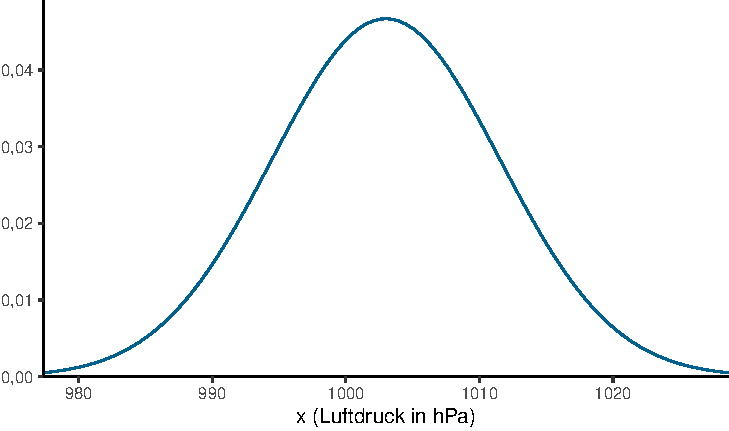
\includegraphics[width=.49\linewidth]{bookdownproj_files/figure-latex/dens-1} 

}

\caption{Theoretische Wahrscheinlichkeitsdichtefunktion des Luftdrucks}\label{fig:dens}
\end{figure}

Wir können auch (analog zu \autoref{eq:norm}) schreiben:

\[
x \sim N(1003, 73)
\]

Daraus ergibt sich für die Standardabweichung \(\sigma\):
\nopagebreak
\[\begin{aligned}
\sigma&=\sqrt{\sigma^2}\\
&=\sqrt{73}\\
&\approx8,54\end{aligned}\]

\hypertarget{unter}{%
\subsubsection{Unterschreitungswahrscheinlichkeit}\label{unter}}

Die einfachste Art der Fragestellung ist nun, mit welcher Wahrscheinlichkeit ein bestimmter Wert \(x_p\) unterschritten wird.

Nehmen wir an, es sei gefragt, mit welcher Wahrscheinlichkeit zu einem beliebigen Zeitpunkt der Luftdruck weniger als 1015 hpa beträgt. Anders gesagt interessiert uns der Anteil der Fläche unter der Verteilung, der zwischen \(-\infty\) und \(x_p=1015\) liegt (s. \autoref{fig:unter}).

\begin{figure}[H]

{\centering 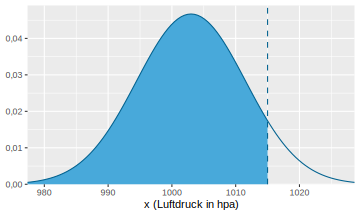
\includegraphics[width=.49\linewidth]{bookdownproj_files/figure-latex/unter-1} 

}

\caption{Unterschreitung eines Messwerts}\label{fig:unter}
\end{figure}

Um den entsprechenden Wert für \(P(x < x_p)\) (also die Wahrscheinlichkeit, dass ein zufälliges \(x\) unser Perzentil \(x_p\) unterschreitet) in Erfahrung zu bringen, müssen wir die Verteilung zunächst standardisieren. Der Wert \(z_p\) ergibt sich aus der Formel für die \(z\)-Transformation, diesmal jedoch mit \(\mu\) statt \(\bar{x}\) und \(\sigma\) statt \(s\), da es sich um die Grundgesamtheit handelt:

\[\begin{aligned}
    z_p &= \frac{x_p-\mu}{\sigma} \\[4pt]
        &\approx \frac{1015-1003}{8,54}\\[4pt]
        &\approx 1,41
  \end{aligned}
\]

Graphisch ist das standardisierte Perzentil in \autoref{fig:z} dargestellt.

\begin{figure}[H]

{\centering 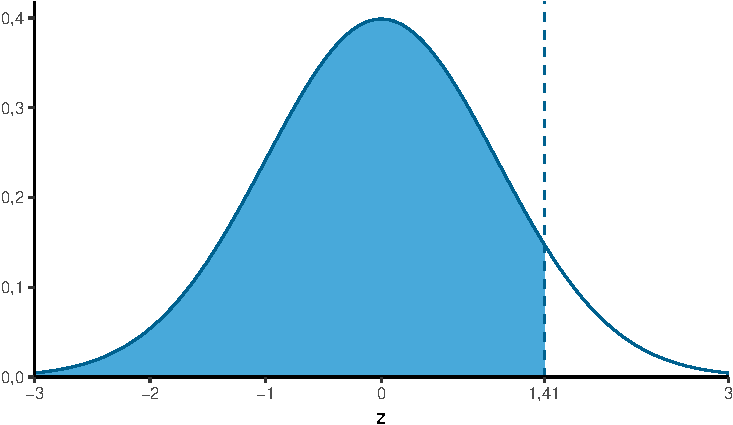
\includegraphics[width=.49\linewidth]{bookdownproj_files/figure-latex/z-1} 

}

\caption{Standardnormalverteilung des Luftdrucks}\label{fig:z}
\end{figure}

Die \protect\hyperlink{ptab}{Tabelle im Anhang} gibt für \(z\)-Werte die Wahrscheinlichkeit ihrer Unterschreitung in ener Normalverteilung an. Diese Wahrscheinlichkeit kann notiert werden als \(P(z<z_p)\).

Der \protect\hyperlink{ptab}{Tabelle im Anhang} können wir den Wert \(P(z < 1,41) \approx 0,9207\) entnehmen. Die Wahrscheinlichkeit, dass der Luftdruck zu einem zufälligen Zeitpunkt weniger als 1015 hPA beträgt, ist somit 92,07\%.

\begin{rtip}
In R lässt sich die Unterschreitungswahrscheinlichkeit eines $z$-Werts mit dem Befehl {\tt pnorm()} ermitteln.
\end{rtip}

\hypertarget{uxfcberschreitungswahrscheinlichkeit}{%
\paragraph{Überschreitungswahrscheinlichkeit}\label{uxfcberschreitungswahrscheinlichkeit}}

Wird nach der Wahrscheinlichkeit der Überschreitung eines Werts gefragt, ist in anderen Worten die Fläche unter der Wahrscheinlichkeitsdichtefunktion zwischen \(x_p\) und \(\infty\) gemeint. Wir bleiben bei unserem Beispiel \(x_p=1015\) (s. \autoref{fig:ueber}).

\begin{figure}[h]

{\centering 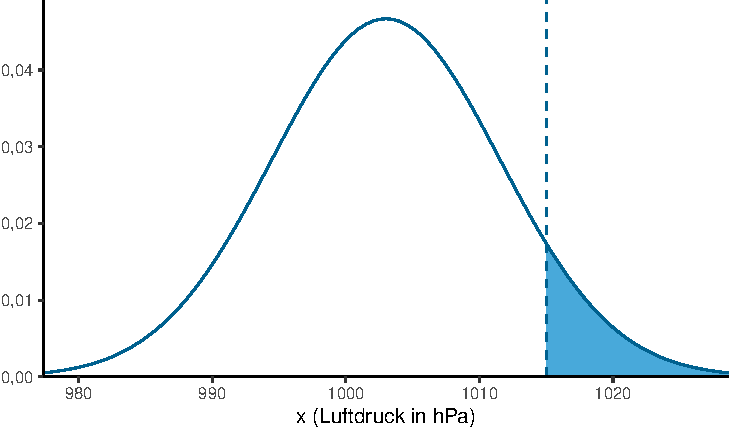
\includegraphics[width=.49\linewidth]{bookdownproj_files/figure-latex/ueber-1} 

}

\caption{Überschreitung eines Messwerts}\label{fig:ueber}
\end{figure}

Hier können wir genauso wie bei der Unterschreitung \(z_p=1,41\) errechnen.

Jetzt stehen wir zunächst vor dem Problem, dass die \(p\)-Werte in der Tabelle immer die Wahrscheinlichkeit der Unterschreitung darstellen. Wir wissen jedoch: Die gesamte Fläche unter der Verteilung ist 1, und die Wahrscheinlichkeiten der Unter- und Überschreitung sind komplementär, d.h. einer von beiden Fällen tritt sicher (mit einer Wahrscheinlichkeit von 100\%) ein. (Den Sonderfall \(x=x_p\) können wir bei stetigen Variablen vernachlässigen.)

Hieraus ergibt sich ganz allgemein:

\[
  \begin{aligned}
    P(x \geq x_p) = 1-P(x<x_p)
  \end{aligned}
\]\{\#eq:ueber\}

Und für unser Beispiel:

\[
  \begin{aligned}
    P(x \geq 1015) &= 1-P(x < 1015) \\
    &\approx1-P(z < 1,41)\\
    &\approx1-0,9207\\
    &= 0,0793
  \end{aligned}
\]

In 7,93\% der Fälle beträgt der Luftdruck also über 1015 hPA.

\hypertarget{negativer-z-wert}{%
\paragraph{\texorpdfstring{Negativer \(z\)-Wert}{Negativer z-Wert}}\label{negativer-z-wert}}

Wenn nach der Unterschreitungswahrscheinlichkeit eines unterdurchschnittlichen Werts gefragt ist (z.B. 990 hPA), dann ergibt sich ein negativer Wert für \(z_p\):

\begin{equation}
  \begin{aligned}
    z_p &= \frac{x_p-\mu}{\sigma} \\[4pt]
        &= \frac{990-1003}{8,54} \\[4pt]
        &\approx -1,52
  \end{aligned}
\end{equation}

Die \protect\hyperlink{ptab}{Tabelle im Anhang} enthält keine \(p\) für negative \(z_p\). Da die Standardnormalverteilung jedoch um \(z=0\) symmetrisch ist, gilt ganz allgemein:

\[
  \begin{aligned}
    P(z < -z_p) = 1 - P(z < z_p)
  \end{aligned}
\]\{\#eq:neg\}

Für unser Beispiel ergibt sich (mit dem Wert \(P(z < 1,52) = 0,9357\) aus der Tabelle):

\[
  \begin{aligned}
    P(z < -1,52) &= 1 - P(z < 1,52) \\
    &\approx 1-0,9357 \\
    &=0,0643
  \end{aligned}
\]

Ein Luftdruck von 990 hPa wird also nur in ca. 6,43\% der Fälle unterschritten.

\begin{rtip}
Der Befehl {\tt pnorm()} funktioniert auch mit negativen $z$-Werten.
\end{rtip}

\hypertarget{wert-in-einem-intervall}{%
\paragraph{Wert in einem Intervall}\label{wert-in-einem-intervall}}

Nun wollen wir wissen, mit welcher Wahrscheinlichkeit ein zufälliger Meßwert zwischen 1005 und 1015 hPa liegt. Graphisch ist dies in \autoref{fig:intervall} aufbereitet.

\begin{figure}[h]

{\centering 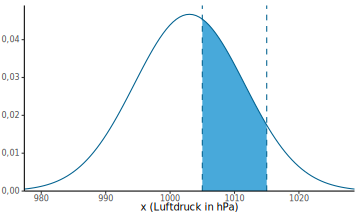
\includegraphics[width=.49\linewidth]{bookdownproj_files/figure-latex/intervall-1} 

}

\caption{Messwertintervall}\label{fig:intervall}
\end{figure}

Rechnerisch müssen wir also von den (günstigen) Fällen, in denen 1015 hPA unterschritten werden, noch jene (ungünstige) Fälle abziehen, in denen die 1005 hPA \emph{ebenfalls} unterschritten werden.

Ganz allgemein heißt das für die Untergrenze \(x_u\) und die Obergrenze \(x_o\):

\[
  \begin{aligned}
    P(x_{u} \leq x < x_{o}) = P(x < x_{o}) - P(x < x_{u})
  \end{aligned}
\]\{\#eq:intervall\}

Für unseren Fall ist \(x_u=1005\) und \(x_o=1015\). In den \protect\hyperlink{unter}{vorherigen Aufgaben} haben wir \(z_o\approx1,41\) bereits ermittelt. Wir müssen aber noch \(z_u\) ermitteln:

\[
  \begin{aligned}5
    z_u &= \frac{x_u-\mu}{\sigma} \\[4pt]
        &= \frac{1005-1003}{8,54}  \\[4pt]
        &\approx 0,23
  \end{aligned}
\]

Dann können wir die entsprechende Wahrscheinlichkeit berechnen, indem wir wieder die Werte aus der \protect\hyperlink{ptab}{Tabelle im Anhang} einsetzen:

\[
  \begin{aligned}
    P(1005 \leq x < 1015) &= P(x < 1015) - P(x < 1005) \\
    &\approx P(z < 1,41) - P(z < 0,23) \\
    &\approx 0,9207- 0,5910  \\
    &= 0,3297
  \end{aligned}
\]

Der Luftdruck liegt also mit einer Wahrscheinlichkeit von 32,97\% zwischen 1005 und 1015 hPa.

\hypertarget{gesuchter-wert-bei-gegebener-wahrscheinlichkeit}{%
\paragraph{Gesuchter Wert bei gegebener Wahrscheinlichkeit}\label{gesuchter-wert-bei-gegebener-wahrscheinlichkeit}}

Die Fragerichtung lässt sich umdrehen: Welche Marke wird beim Messen des Luftdrucks nur in 5\% der Fälle überschritten?

5\% Überschreitungswahrscheinlichkeit entsprechen einer Unterschreitungswahrscheinlichkeit von 95\%. Welcher Wert wird also mit 95\% Wahrscheinlichkeit unterschritten?

Der Tabelle entnehmen wir, dass einer Unterschreitungswahrscheinlichkeit von 0,95 ein \(z\)-Wert zwischen 1,64 und 1,65 entspricht. Da es bei dieser Fragestellungen oft darum geht, einen ``kritischen'' Wert zu nennen, der nur in Ausnahmefällen überschritten wird, nehmen wir hier üblicherweise den extremeren Wert, also \(z_{95\%}\approx 1,65\).

Mit der umgekehrten \(z\)-Transformation erhalten wir:

\[
  \begin{aligned}
    x_{95\%}&=z_{95\%}\cdot \sigma + \mu \\
       &\approx 1,65\cdot 8,54 + 1003\\
       &\approx 1017,10
  \end{aligned}
\]

Die Marke von 1017,10 hPa wird also nur in 5\% der Fälle überschritten.

\begin{rtip}
Das Perzentil für eine gegebene Unterschreitungswahrscheinlichkeit lässt sich in R mit {\tt qnorm()} bestimmen.
\end{rtip}

\hypertarget{gesuchte-grenzwerte-eines-intervalls}{%
\paragraph{Gesuchte Grenzwerte eines Intervalls}\label{gesuchte-grenzwerte-eines-intervalls}}

Eine übliche Art der Fragestellung ist auch: Zwischen welchen beiden Werten liegen die mittleren 85\% der Fälle (s. Abbiddung \ref{fig:mitte})?

\begin{figure}[h]

{\centering 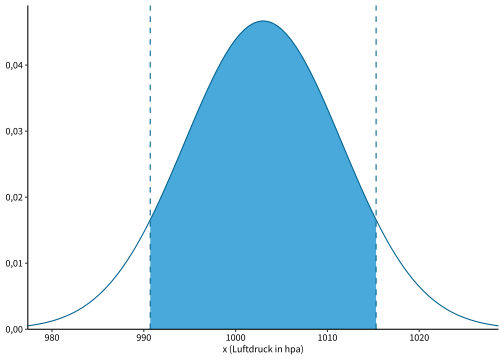
\includegraphics[width=.49\linewidth]{bookdownproj_files/figure-latex/mitte-1} 

}

\caption{Die mittleren 85\% der Normalverteilung}\label{fig:mitte}
\end{figure}

Da die Verteilung symmetrisch ist, teilen sich die ungünstigen 15\% der Fälle gleichmäßig an den oberen und unteren Rand der Verteilung auf. Die Obergrenze \(x_o\) ist also der Wert, der zu 7,5\% über- und damit zu 92,5\% unterschritten wird.

Der Tabelle entnehmen wir den Wert \(z_o=z_{92,5\%}\approx1,44\).

Die Untergrenze ist entsprechend der Wert, der in 7,5\% der Fälle unterschritten wird.

Der Wert für \(z_u=z_{7,5\%}\) ist in der Tabelle nicht enthalten. Weil die Verteilung aber symmetrisch ist, wissen wir uns zu helfen:

\[
  \begin{aligned}
    z_u=z_{7,5\%}=-z_{92,5\%}\approx-1,44
  \end{aligned}
\]

Die absoluten Werte ergeben sich schließlich aus:
\[
  \begin{aligned}
    x_u&=z_u\cdot \sigma + \mu \\
    &\approx-1,44 \cdot 8,54 + 1003\\
    &\approx990,70
  \end{aligned}
\]

Und:
\[
  \begin{aligned}
    x_o&=z_o\cdot \sigma + \mu  \\
    &\approx1,44 \cdot 8,54 + 1003\\
    & \approx 1015,30
  \end{aligned}
\]

Die mittleren 85\% der Messwerte liegen also zwischen 990,7 und 1015,3 hPa.

\hypertarget{aufgaben-2}{%
\subsection{Aufgaben}\label{aufgaben-2}}

Die folgenden Aufgaben sind zur eigenständigen Überprüfung Ihrer Lernleistung gedacht (als Vor- oder Nachbereitung der Vorlesung, oder als Klausurübung) und nicht etwa als Hausaufgabe.

\hypertarget{aufgabe-1-2}{%
\subsubsection{Aufgabe 1}\label{aufgabe-1-2}}

Deiche werden durch Wasserdruck bei Hochwasser belastet und dadurch beschädigt. Bei einem 12 m hohen Deich gilt als kritische Marke ein Wasserstand von 10 m. Die jährlichen Höchstwasserstände des Flusses sind normalverteilt mit einem Mittelwert von 9,01 m und einer Standardabweichung von 2,23 m.

In den folgenden Teilaufgaben beantworten wir Schritt für Schritt die Frage, wie wahrscheinlich es (für ein beliebiges Jahr) ist, dass der Deich das jährliche Hochwasser ohne Beschädigung übersteht, d.h. dass ein Höchstwasserstand von 10 m oder weniger eintritt.

\begin{enumerate}
\def\labelenumi{\alph{enumi})}
\tightlist
\item
  Zeichnen Sie die Wahrscheinlichkeitsdichtefunktion (ganz grob, ohne y-Achse).
\item
  Markieren Sie den kritischen Wert 10 m.
\item
  Welchem \(z\)-Wert entspricht die kritische Marke von 10 m?
\item
  Mit welcher Wahrscheinlichkeit bleibt der Deich in einem gegebenen Jahr unbeschädigt (Höchstwasserstand unter der kritischen Marke von 10 m)?
\end{enumerate}

\hypertarget{aufgabe-2-2}{%
\subsubsection{Aufgabe 2}\label{aufgabe-2-2}}

Wir bleiben beim Deich aus Aufgabe 1.

\begin{enumerate}
\def\labelenumi{\alph{enumi})}
\tightlist
\item
  Mit welcher Wahrscheinlichkeit wird der Deich beschädigt (Wasserstand über 10 m)?
\item
  Mit welcher Wahrscheinlichkeit wird der Deich nicht nur beschädigt, sondern läuft über (Wasserstand über 12 m)?
\item
  Mit welcher Wahrscheinlichkeit wird der Deich beschädigt, läuft aber nicht über (Wasserstand zwischen 10 und 12 m)?
\item
  In welchen Grenzen liegen die mittleren 80\% der Hochwasserstände?
\end{enumerate}

\hypertarget{aufgabe-3}{%
\subsubsection{Aufgabe 3}\label{aufgabe-3}}

Es ist ein neuer Deich zu bauen, der so sicher sein soll, dass er nur alle 200 Jahre vom Hochwasser übertreten wird.

\begin{enumerate}
\def\labelenumi{\alph{enumi})}
\tightlist
\item
  Welcher Wahrscheinlichkeitswert \(p=P(x < x_p)\) ist anzuwenden, d.h. wie wahrscheinlich ist die \emph{Unterschreitung} eines ``zweihundertjähriges Hochwassers''?
\item
  Mit welchem \(z\)-Wert korrespondiert der gesuchte Wert \(x_p\)?
\item
  Wie hoch muss dieser Deich sein? (Welcher Wert \(x_p\) entspricht diesem \(z_p\)?)
\end{enumerate}

\hypertarget{aufgabe-4}{%
\subsubsection{Aufgabe 4}\label{aufgabe-4}}

Die jährlichen Niederschlagsmengen in Mittelstedt betragen im Mittel 400 mm bei annähernder Normalverteilung und einer Standardabweichung von 100 mm.

\begin{enumerate}
\def\labelenumi{\alph{enumi})}
\tightlist
\item
  Wie groß ist die Wahrscheinlichkeit, dass mehr als 500 mm Niederschlag fallen?
\item
  Wie oft pro hundert Jahre kann mit weniger als 200 mm Niederschlag gerechnet werden?
\item
  Mit welcher Wahrscheinlichkeit fallen zwischen 200 mm und 550 mm Niederschlag?
\item
  Welche Niederschlagsmenge wird wahrscheinlich in nur 2 von 100 Jahren übertroffen?
\item
  In welchen Grenzen liegen die mittleren 75\% der jährlichen Niederschlagsmenge?
\end{enumerate}

\hypertarget{tipps-zur-vertiefung-2}{%
\subsection{Tipps zur Vertiefung}\label{tipps-zur-vertiefung-2}}

\hypertarget{variationskoeffizient-1}{%
\subsubsection{Variationskoeffizient}\label{variationskoeffizient-1}}

\begin{itemize}
\tightlist
\item
  Kapitel 4.2.2 in \protect\hyperlink{ref-bahrenberg}{Bahrenberg, Giese und Nipper} (\protect\hyperlink{ref-bahrenberg}{2010})
\item
  YouTube-Kanal ``Kurzes Tutorium Statistik'': \href{https://www.youtube.com/watch?v=3oZrS3ZWVcA}{Streumaße - Varianz, Standardabweichung, Variationskoeffizient und mehr!}
\end{itemize}

\hypertarget{z-transformation-1}{%
\subsubsection{z-Transformation}\label{z-transformation-1}}

\begin{itemize}
\tightlist
\item
  Kapitel 2.4 in \protect\hyperlink{ref-bortz}{Bortz und Schuster} (\protect\hyperlink{ref-bortz}{2010})
\item
  Kapitel 4.2.2 in \protect\hyperlink{ref-bahrenberg}{Bahrenberg, Giese und Nipper} (\protect\hyperlink{ref-bahrenberg}{2010})
\item
  Kapitel 3.3.3 in \protect\hyperlink{ref-benninghaus}{Benninghaus} (\protect\hyperlink{ref-benninghaus}{2007})
\item
  YouTube-Kanal ``Methodenlehre Mainz'': \href{https://www.youtube.com/watch?v=AiucvUlIP8k}{WT.012.09 Äpfel mit Birnen vergleichen: Die z-Standardisierung}
\end{itemize}

\hypertarget{normalverteilung-1}{%
\subsubsection{Normalverteilung}\label{normalverteilung-1}}

\begin{itemize}
\tightlist
\item
  Kapitel 5.4 in \protect\hyperlink{ref-bortz}{Bortz und Schuster} (\protect\hyperlink{ref-bortz}{2010})
\item
  Kapitel 5.2.2 in \protect\hyperlink{ref-bahrenberg}{Bahrenberg, Giese und Nipper} (\protect\hyperlink{ref-bahrenberg}{2010})
\item
  YouTube-Kanal ``Mathe by Daniel Jung'': \href{https://www.youtube.com/watch?v=_f1vgWUiavY}{Was ist die Normalverteilung, Gauß-Verteilung, Schaubilder, Übersicht}
\end{itemize}

\hypertarget{wahrscheinlichkeitsdichtefunktion}{%
\subsubsection{Wahrscheinlichkeitsdichtefunktion}\label{wahrscheinlichkeitsdichtefunktion}}

\begin{itemize}
\tightlist
\item
  Kapitel 5.3 in \protect\hyperlink{ref-bortz}{Bortz und Schuster} (\protect\hyperlink{ref-bortz}{2010})
\item
  Kapitel 5.2.2 in \protect\hyperlink{ref-bahrenberg}{Bahrenberg, Giese und Nipper} (\protect\hyperlink{ref-bahrenberg}{2010})
\item
  YouTube-Kanal ``Kurzes Tutorium Statistik'': \href{https://www.youtube.com/watch?v=DoHTsDrzAQk}{Zufallsvariable, Massenfunktion, Dichtefunktion und Verteilungsfunktion}
\end{itemize}

\pagebreak

\hypertarget{ptab}{%
\subsection{Anhang: Tabelle Standardnormalverteilung}\label{ptab}}

\begin{multicols}{2}


\begin{center}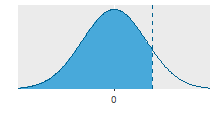
\includegraphics[width=.49\linewidth]{bookdownproj_files/figure-latex/unnamed-chunk-8-1} \end{center}

\[ P(z < -z_p) = 1-P(z< z_p) \]

\end{multicols}

\begin{table}[!h]
\centering
\resizebox{\linewidth}{!}{
\begin{tabular}{>{}r|rrrrrrrrrr}
\toprule
\multicolumn{1}{c}{ } & \multicolumn{10}{c}{$z$ (zweite Nachkommastelle)} \\
\cmidrule(l{3pt}r{3pt}){2-11}
$z$ & 0,00 & 0,01 & 0,02 & 0,03 & 0,04 & 0,05 & 0,06 & 0,07 & 0,08 & 0,09\\
\midrule
\cellcolor{gray!6}{0,0} & \cellcolor{gray!6}{0,5000} & \cellcolor{gray!6}{0,5040} & \cellcolor{gray!6}{0,5080} & \cellcolor{gray!6}{0,5120} & \cellcolor{gray!6}{0,5160} & \cellcolor{gray!6}{0,5199} & \cellcolor{gray!6}{0,5239} & \cellcolor{gray!6}{0,5279} & \cellcolor{gray!6}{0,5319} & \cellcolor{gray!6}{0,5359}\\
0,1 & 0,5398 & 0,5438 & 0,5478 & 0,5517 & 0,5557 & 0,5596 & 0,5636 & 0,5675 & 0,5714 & 0,5753\\
\cellcolor{gray!6}{0,2} & \cellcolor{gray!6}{0,5793} & \cellcolor{gray!6}{0,5832} & \cellcolor{gray!6}{0,5871} & \cellcolor{gray!6}{0,5910} & \cellcolor{gray!6}{0,5948} & \cellcolor{gray!6}{0,5987} & \cellcolor{gray!6}{0,6026} & \cellcolor{gray!6}{0,6064} & \cellcolor{gray!6}{0,6103} & \cellcolor{gray!6}{0,6141}\\
0,3 & 0,6179 & 0,6217 & 0,6255 & 0,6293 & 0,6331 & 0,6368 & 0,6406 & 0,6443 & 0,6480 & 0,6517\\
\cellcolor{gray!6}{0,4} & \cellcolor{gray!6}{0,6554} & \cellcolor{gray!6}{0,6591} & \cellcolor{gray!6}{0,6628} & \cellcolor{gray!6}{0,6664} & \cellcolor{gray!6}{0,6700} & \cellcolor{gray!6}{0,6736} & \cellcolor{gray!6}{0,6772} & \cellcolor{gray!6}{0,6808} & \cellcolor{gray!6}{0,6844} & \cellcolor{gray!6}{0,6879}\\
\addlinespace
0,5 & 0,6915 & 0,6950 & 0,6985 & 0,7019 & 0,7054 & 0,7088 & 0,7123 & 0,7157 & 0,7190 & 0,7224\\
\cellcolor{gray!6}{0,6} & \cellcolor{gray!6}{0,7257} & \cellcolor{gray!6}{0,7291} & \cellcolor{gray!6}{0,7324} & \cellcolor{gray!6}{0,7357} & \cellcolor{gray!6}{0,7389} & \cellcolor{gray!6}{0,7422} & \cellcolor{gray!6}{0,7454} & \cellcolor{gray!6}{0,7486} & \cellcolor{gray!6}{0,7517} & \cellcolor{gray!6}{0,7549}\\
0,7 & 0,7580 & 0,7611 & 0,7642 & 0,7673 & 0,7703 & 0,7734 & 0,7764 & 0,7794 & 0,7823 & 0,7852\\
\cellcolor{gray!6}{0,8} & \cellcolor{gray!6}{0,7881} & \cellcolor{gray!6}{0,7910} & \cellcolor{gray!6}{0,7939} & \cellcolor{gray!6}{0,7967} & \cellcolor{gray!6}{0,7995} & \cellcolor{gray!6}{0,8023} & \cellcolor{gray!6}{0,8051} & \cellcolor{gray!6}{0,8078} & \cellcolor{gray!6}{0,8106} & \cellcolor{gray!6}{0,8133}\\
0,9 & 0,8159 & 0,8186 & 0,8212 & 0,8238 & 0,8264 & 0,8289 & 0,8315 & 0,8340 & 0,8365 & 0,8389\\
\addlinespace
\cellcolor{gray!6}{1,0} & \cellcolor{gray!6}{0,8413} & \cellcolor{gray!6}{0,8438} & \cellcolor{gray!6}{0,8461} & \cellcolor{gray!6}{0,8485} & \cellcolor{gray!6}{0,8508} & \cellcolor{gray!6}{0,8531} & \cellcolor{gray!6}{0,8554} & \cellcolor{gray!6}{0,8577} & \cellcolor{gray!6}{0,8599} & \cellcolor{gray!6}{0,8621}\\
1,1 & 0,8643 & 0,8665 & 0,8686 & 0,8708 & 0,8729 & 0,8749 & 0,8770 & 0,8790 & 0,8810 & 0,8830\\
\cellcolor{gray!6}{1,2} & \cellcolor{gray!6}{0,8849} & \cellcolor{gray!6}{0,8869} & \cellcolor{gray!6}{0,8888} & \cellcolor{gray!6}{0,8907} & \cellcolor{gray!6}{0,8925} & \cellcolor{gray!6}{0,8944} & \cellcolor{gray!6}{0,8962} & \cellcolor{gray!6}{0,8980} & \cellcolor{gray!6}{0,8997} & \cellcolor{gray!6}{0,9015}\\
1,3 & 0,9032 & 0,9049 & 0,9066 & 0,9082 & 0,9099 & 0,9115 & 0,9131 & 0,9147 & 0,9162 & 0,9177\\
\cellcolor{gray!6}{1,4} & \cellcolor{gray!6}{0,9192} & \cellcolor{gray!6}{0,9207} & \cellcolor{gray!6}{0,9222} & \cellcolor{gray!6}{0,9236} & \cellcolor{gray!6}{0,9251} & \cellcolor{gray!6}{0,9265} & \cellcolor{gray!6}{0,9279} & \cellcolor{gray!6}{0,9292} & \cellcolor{gray!6}{0,9306} & \cellcolor{gray!6}{0,9319}\\
\addlinespace
1,5 & 0,9332 & 0,9345 & 0,9357 & 0,9370 & 0,9382 & 0,9394 & 0,9406 & 0,9418 & 0,9429 & 0,9441\\
\cellcolor{gray!6}{1,6} & \cellcolor{gray!6}{0,9452} & \cellcolor{gray!6}{0,9463} & \cellcolor{gray!6}{0,9474} & \cellcolor{gray!6}{0,9484} & \cellcolor{gray!6}{0,9495} & \cellcolor{gray!6}{0,9505} & \cellcolor{gray!6}{0,9515} & \cellcolor{gray!6}{0,9525} & \cellcolor{gray!6}{0,9535} & \cellcolor{gray!6}{0,9545}\\
1,7 & 0,9554 & 0,9564 & 0,9573 & 0,9582 & 0,9591 & 0,9599 & 0,9608 & 0,9616 & 0,9625 & 0,9633\\
\cellcolor{gray!6}{1,8} & \cellcolor{gray!6}{0,9641} & \cellcolor{gray!6}{0,9649} & \cellcolor{gray!6}{0,9656} & \cellcolor{gray!6}{0,9664} & \cellcolor{gray!6}{0,9671} & \cellcolor{gray!6}{0,9678} & \cellcolor{gray!6}{0,9686} & \cellcolor{gray!6}{0,9693} & \cellcolor{gray!6}{0,9699} & \cellcolor{gray!6}{0,9706}\\
1,9 & 0,9713 & 0,9719 & 0,9726 & 0,9732 & 0,9738 & 0,9744 & 0,9750 & 0,9756 & 0,9761 & 0,9767\\
\addlinespace
\cellcolor{gray!6}{2,0} & \cellcolor{gray!6}{0,9772} & \cellcolor{gray!6}{0,9778} & \cellcolor{gray!6}{0,9783} & \cellcolor{gray!6}{0,9788} & \cellcolor{gray!6}{0,9793} & \cellcolor{gray!6}{0,9798} & \cellcolor{gray!6}{0,9803} & \cellcolor{gray!6}{0,9808} & \cellcolor{gray!6}{0,9812} & \cellcolor{gray!6}{0,9817}\\
2,1 & 0,9821 & 0,9826 & 0,9830 & 0,9834 & 0,9838 & 0,9842 & 0,9846 & 0,9850 & 0,9854 & 0,9857\\
\cellcolor{gray!6}{2,2} & \cellcolor{gray!6}{0,9861} & \cellcolor{gray!6}{0,9864} & \cellcolor{gray!6}{0,9868} & \cellcolor{gray!6}{0,9871} & \cellcolor{gray!6}{0,9875} & \cellcolor{gray!6}{0,9878} & \cellcolor{gray!6}{0,9881} & \cellcolor{gray!6}{0,9884} & \cellcolor{gray!6}{0,9887} & \cellcolor{gray!6}{0,9890}\\
2,3 & 0,9893 & 0,9896 & 0,9898 & 0,9901 & 0,9904 & 0,9906 & 0,9909 & 0,9911 & 0,9913 & 0,9916\\
\cellcolor{gray!6}{2,4} & \cellcolor{gray!6}{0,9918} & \cellcolor{gray!6}{0,9920} & \cellcolor{gray!6}{0,9922} & \cellcolor{gray!6}{0,9925} & \cellcolor{gray!6}{0,9927} & \cellcolor{gray!6}{0,9929} & \cellcolor{gray!6}{0,9931} & \cellcolor{gray!6}{0,9932} & \cellcolor{gray!6}{0,9934} & \cellcolor{gray!6}{0,9936}\\
\addlinespace
2,5 & 0,9938 & 0,9940 & 0,9941 & 0,9943 & 0,9945 & 0,9946 & 0,9948 & 0,9949 & 0,9951 & 0,9952\\
\cellcolor{gray!6}{2,6} & \cellcolor{gray!6}{0,9953} & \cellcolor{gray!6}{0,9955} & \cellcolor{gray!6}{0,9956} & \cellcolor{gray!6}{0,9957} & \cellcolor{gray!6}{0,9959} & \cellcolor{gray!6}{0,9960} & \cellcolor{gray!6}{0,9961} & \cellcolor{gray!6}{0,9962} & \cellcolor{gray!6}{0,9963} & \cellcolor{gray!6}{0,9964}\\
2,7 & 0,9965 & 0,9966 & 0,9967 & 0,9968 & 0,9969 & 0,9970 & 0,9971 & 0,9972 & 0,9973 & 0,9974\\
\cellcolor{gray!6}{2,8} & \cellcolor{gray!6}{0,9974} & \cellcolor{gray!6}{0,9975} & \cellcolor{gray!6}{0,9976} & \cellcolor{gray!6}{0,9977} & \cellcolor{gray!6}{0,9977} & \cellcolor{gray!6}{0,9978} & \cellcolor{gray!6}{0,9979} & \cellcolor{gray!6}{0,9979} & \cellcolor{gray!6}{0,9980} & \cellcolor{gray!6}{0,9981}\\
2,9 & 0,9981 & 0,9982 & 0,9982 & 0,9983 & 0,9984 & 0,9984 & 0,9985 & 0,9985 & 0,9986 & 0,9986\\
\addlinespace
\cellcolor{gray!6}{3,0} & \cellcolor{gray!6}{0,9987} & \cellcolor{gray!6}{0,9987} & \cellcolor{gray!6}{0,9987} & \cellcolor{gray!6}{0,9988} & \cellcolor{gray!6}{0,9988} & \cellcolor{gray!6}{0,9989} & \cellcolor{gray!6}{0,9989} & \cellcolor{gray!6}{0,9989} & \cellcolor{gray!6}{0,9990} & \cellcolor{gray!6}{0,9990}\\
\bottomrule
\end{tabular}}
\end{table}

Quelle: Werte wurden automatisch mit der Funktion \texttt{pnorm} aus R (\protect\hyperlink{ref-r}{R Core Team 2018}) generiert.

\pagebreak

\hypertarget{quellen-2}{%
\subsection{Quellen}\label{quellen-2}}

\hypertarget{schuxe4tzstatistik-1}{%
\section{Schätzstatistik}\label{schuxe4tzstatistik-1}}

\hypertarget{lernziele-dieser-sitzung-3}{%
\subsection{Lernziele dieser Sitzung}\label{lernziele-dieser-sitzung-3}}

Sie können\ldots{}

\begin{itemize}
\tightlist
\item
  eine Punktschätzung für \(\mu\) und \(\sigma\) durchführen.
\item
  den Standardfehler der Stichprobenverteilung von \(\bar{x}\) bestimmen.
\item
  eine Intervallschätzung für \(\mu\) durchführen.
\end{itemize}

\hypertarget{stichprobenverteilung}{%
\subsection{Stichprobenverteilung}\label{stichprobenverteilung}}

\begin{quote}
Die Stichprobenverteilung ist eine theoretische Verteilung, welche die möglichen Ausprägungen eines statistischen Kennwertes (z.B. \(\bar{x}\)) sowie deren Auftretenswahrscheinlichkeit beim Ziehen von Zufallsstichproben des Umfanges \(n\) beschreibt. (\protect\hyperlink{ref-bortz}{Bortz und Schuster 2010}: 83)
\end{quote}

Hier ist zunächst die theoretische Verteilung des Mittelwerts einer Stichprobe relevant. Insbesondere interessiert uns, wie sich die theoretische Verteilung des Mittelwerts abhängig von der Stichprobengröße verhält.

\hypertarget{szenario-1-normalverteilte-grundgesamtheit}{%
\subsubsection{Szenario 1: Normalverteilte Grundgesamtheit}\label{szenario-1-normalverteilte-grundgesamtheit}}

Die Grundgesamtheit (Population) einer Variable \(x\) sei normalverteilt mit \(\mu=50\) und \(\sigma^2=25\). Wir können also schreiben:

\nopagebreak

\[ x \sim N(50,25) \]

Die Standardabweichung der Population beträgt entsprechend:

\nopagebreak

\[\begin{aligned}
\sigma&=\sqrt{\sigma^2}\\[4pt]
&=\sqrt{25}=5\end{aligned}\]

Graphisch ist die Dichtefunktion der Verteilung in \autoref{fig:pop} veranschaulicht.

\begin{figure}[h]

{\centering 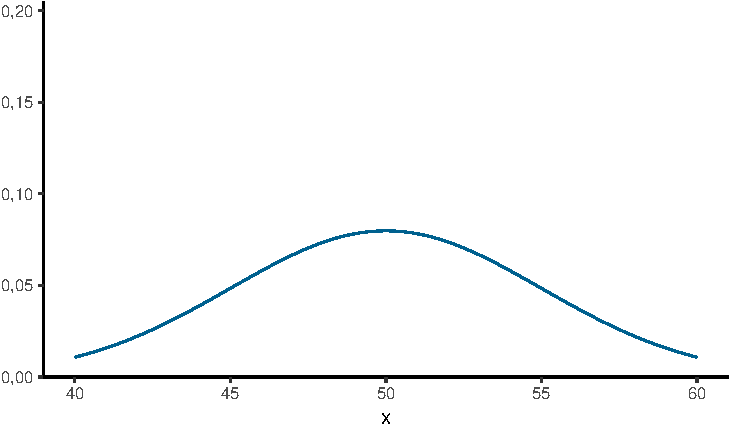
\includegraphics[width=.49\linewidth]{bookdownproj_files/figure-latex/pop-1} 

}

\caption{Dichtefunktion der Grundgesamtheit}\label{fig:pop}
\end{figure}

Wenn eine einzelne Stichprobe der Größe \(n=3\) aus dieser Verteilung gezogen würde, hätte sie drei konkrete Werte (\(x_1\), \(x_2\) und \(x_3\)) sowie ein konkretes arithmetisches Mittel (\(\bar{x}\)).

Es lässt sich jedoch auch eine Wahrscheinlichkeitsdichtefunktion der Mittelwerte \emph{aller theoretisch möglichen Stichproben} der Größe \(n=3\) (und zusätzlich der Größe \(n=6\)) zeichnen (s. \autoref{fig:stich}).

\begin{figure}[h]

{\centering 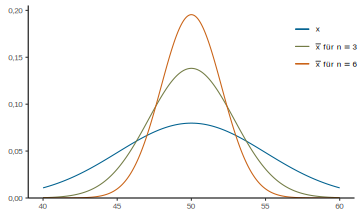
\includegraphics[width=.49\linewidth]{bookdownproj_files/figure-latex/stich-1} 

}

\caption{Dichtefunktionen der Stichprobenverteilungen}\label{fig:stich}
\end{figure}

\hypertarget{erwartungswert}{%
\paragraph{Erwartungswert}\label{erwartungswert}}

Es fällt auf, dass die Stichprobenverteilungen für \(\bar{x}\) normalverteilt sind und um das arithmetische Mittel der Grundgesamtheit (\(\mu\)) symmetrisch sind.

Das arithmetische Mittel der Stichprobenverteilung \(\mu_{\bar{x}}\) wird auch als \textbf{Erwartungswert} (engl. \emph{expected value}) von \(\bar{x}\) bezeichnet. Es gilt:

\nopagebreak

\[
\mu_{\bar{x}} = \mu
\]\{\#eq:mean\}

Wir können auch sagen: \(\bar{x}\) ist ein ``ertwartungstreuer'' Schätzparameter für \(\mu\); nicht weil er in der Empirie zwangsläufig identisch mit \(\mu\) wäre, sondern weil er mit zunehmender Stichprobengröße immer stärker zu \(\mu\) tendiert.

\hypertarget{standardfehler}{%
\paragraph{Standardfehler}\label{standardfehler}}

Zusätzlich fällt in \autoref{fig:stich} auf: Je größer die Stichprobe, desto gestauchter die Dichtekurve der Stichprobenverteilung: Die theoretische Verteilung von \(\bar{x}\) bei \(n=6\) weist eine kleinere Varianz auf als bei \(n=3\). Das ist einigermaßen intuitiv, denn wir können uns vorstellen, dass das arithmetische Mittel \(\bar{x}\) bei steigender Stichprobengröße ein immer präziserer Schätzwert für \(\mu\) wird.

Die Varianz der Stichprobenverteilung für \(\bar{x}\) bezeichnen wir mit \(\sigma^2_{\bar{x}}\). Sie hängt von der Varianz der Population ab und ist invers proportional zur Stichprobengröße. Es gilt:

\nopagebreak

\[
\sigma^2_{\bar{x}} = \frac{\sigma^2}{n}
\] \{\#eq:var\}

Die Standardabweichung der Stichprobenverteilung (\(\sigma_{\bar{x}}\)) wird auch Standardfehler (engl. \emph{standard error}) genannt. Durch Wurzelziehen ergibt sich:

\nopagebreak

\[
\sigma_{\bar{x}} = \frac{\sigma}{\sqrt{n}}
\]\{\#eq:sd\}

Zusammenfassend lässt sich sagen:

\nopagebreak

\[\begin{aligned}
\bar{x} \sim N(\mu, {\textstyle \frac{\sigma^2}{n}}) \quad \textrm{für} \quad x\sim N(\mu, \sigma^2)
\end{aligned}\]\{\#eq:norm\}

\hypertarget{szenario-2-nicht-normalverteilte-grundgesamtheit}{%
\subsubsection{Szenario 2: Nicht normalverteilte Grundgesamtheit}\label{szenario-2-nicht-normalverteilte-grundgesamtheit}}

Die Gleichungen \ref{eq:mean}, \ref{eq:var} und \ref{eq:sd} gelten uneingeschränkt auch für die Stichprobenverteilungen von nicht normalverteilten Populationen. Nur die Normalverteilung der Stichprobenverteilung (\autoref{eq:norm}) ist bei nicht normalverteilten Grundgesamtheiten grundsätzlich nicht gegeben.

Das zentrale Grenzwerttheorem (engl. \emph{central limit theorem}) besagt jedoch:

\begin{quote}
Die Verteilung von Mittelwerten aus Stichproben des Umfangs \(n\), die derselben Grundgesamtheit entnommen wurden, geht mit wachsendem Stichprobenumfang in eine Normalverteilung über. (\protect\hyperlink{ref-bortz}{Bortz und Schuster 2010}: 86)
\end{quote}

\autoref{fig:beta} veranschaulicht diesen Effekt für eine nicht normalverteilte Grundgesamtheit.

\begin{figure}[h]

{\centering 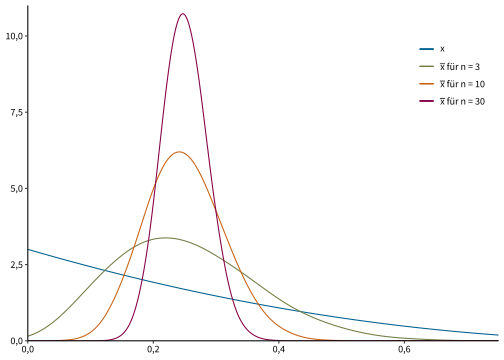
\includegraphics[width=.49\linewidth]{bookdownproj_files/figure-latex/beta-1} 

}

\caption{Stichprobenverteilung bei nicht normalverteilter Population}\label{fig:beta}
\end{figure}

In der Praxis gilt die Faustregel: Ab einer Stichprobengröße von \(n=30\) können wir statistische Verfahren anwenden, die von einer theoretischen Normalverteilung von \(\bar{x}\) ausgehen -- und zwar \emph{unabhängig} von der Verteilung der Grundgesamtheit.

\hypertarget{punktschuxe4tzung}{%
\subsection{Punktschätzung}\label{punktschuxe4tzung}}

Bei statistischen Untersuchungen geht es oft darum, ausgehend von der empirischen Verteilung einer Stichprobe auf Parameter der Grundgesamtheit zu schließen.

Die Punktschätzung (engl. \emph{point estimation}) ist dabei eine vergleichsweise einfache und intuitive Vorgehensweise.

\hypertarget{punktschuxe4tzung-des-arithmetischen-mittels}{%
\subsubsection{Punktschätzung des arithmetischen Mittels}\label{punktschuxe4tzung-des-arithmetischen-mittels}}

Wenn eine Stichprobe vorliegt, dann ist ihr arithmetisches Mittel (\(\bar{x}\)) als erwartungstreuer Punktschätzer der wahrscheinlichste Wert für das arithmetische Mittel der Grundgesamtheit (\(\mu\)).

Beispiel:

\begin{itemize}
\tightlist
\item
  Zehn Studierende der Humangeographie werden zufällig ausgewählt, um ihre Pendelzeit zum IG-Farben-Campus zu erfassen.
\item
  Die Angaben in Minuten lauten:
  \texttt{22\ 26\ 12\ 23\ 48\ 31\ 15\ 71\ 17\ 35}
\item
  Das arithmetische Mittel der Messreihe lässt sich -- wie in Sitzung 2 ausführlich besprochen -- berechnen: \(\bar{x}=30\)
\item
  Da es sich um eine erwartungstreue Schätzgröße (und eine valide Zufallsstichprobe) handelt, kann die durchschnittliche Pendelzeit \emph{aller} Studierenden der Humangeographie auf \(\mu=30\) Minuten geschätzt werden.
\end{itemize}

Gleichzeitig wissen wir jedoch, dass diese Punktschätzung des arithmetischen Mittels vermutlich nicht ganz präzise ist, sondern einem Standardfehler (\(\sigma_{\bar{x}}\)) unterliegt. Woher wissen wir, wie groß dieser Standardfehler ist (und wie unpräzise damit unsere Schätzung)?

\hypertarget{schuxe4tzung-des-standardfehlers}{%
\subsubsection{Schätzung des Standardfehlers}\label{schuxe4tzung-des-standardfehlers}}

Wir führen das obige Beispiel fort:

\begin{itemize}
\tightlist
\item
  Die Varianz der Stichprobe können wir berechnen: \(s^2\approx319{,}78\) (s. Sitzung 2).
\item
  Dabei handelt es sich ebenfalls um einen erwartungstreuen Punktschätzer für die Varianz der Grundgesamtheit (\(\sigma^2\)).
\item
  Die Varianz der Grundgesamtheit kann also auch auf \(\sigma^2=s^2\approx319{,}78\) geschätzt werden.
\item
  Analog können wir die Standardabweichung der Population auf \(\sigma=s\approx17,88\) schätzen.
\item
  Den Standardfehler können wir mit diesem Schätzwert anhand \autoref{eq:sd} berechnen. Allerdings benutzen wir statt \(\sigma_{\bar{x}}\) das Symbol \(s_{\bar{x}}\), da es sich um einen Schätzwert handelt:
\end{itemize}

\nopagebreak

\[\begin{aligned}
s_{\bar{x}} &= \frac{s}{\sqrt{n}}\\[4pt]
&\approx \frac{17{,}88}{\sqrt{10}}\approx5{,}65
\end{aligned}\]

Je größer die Stichprobe, desto genauer lassen sich also Parameter der Population schätzen. Die statistische Antwort auf die Frage, wie groß die Stichprobe denn sein müsse, lautet demnach zunächst immer: Möglichst groß!

Bemerkernswert ist jedoch, dass dabei die Größe der Grundgesamtheit (\(N\), im Beispiel die Anzahl aller Studierenden der Humangeographie) bei diesen Überlegungen überhaupt keine Rolle spielt.

\hypertarget{intervallschuxe4tzung}{%
\subsection{Intervallschätzung}\label{intervallschuxe4tzung}}

Um eine Intervallschätzung durchführen zu können, muss:

\begin{itemize}
\tightlist
\item
  die Standardabweichung der Grundgesamtheit \(\sigma\) bekannt und
\item
  die theoretische Verteilung von \(\bar{x}\) normalverteilt sein. Das bedeutet:

  \begin{itemize}
  \tightlist
  \item
    \emph{Entweder} es ist bekannt, dass die Grundgesamtheit normalverteilt ist
  \item
    \emph{Und/oder} die Stichprobengröße ist \(n\geq30\)
  \end{itemize}
\end{itemize}

Für das obige Beispiel der Pendelzeiten wissen wir nicht, wie die Verteilung der Grundgesamtheit aussieht, und die Stichprobengröße (\(n=10\)) ist kleiner als 30. Eine Intervallschätzung können wir hier also nicht durchführen!

Auch bei der Intervallschätzung (engl. \emph{interval estimation}) geht es darum, das arithmetische Mittel der Population (\(\mu\)) zu schätzen. Allerdings geben wir nicht einfach nur den wahrscheinlichsten Wert an, sondern einen Bereich (ein \emph{Intervall}), in dem \(\mu\) mit einer bestimmten Wahrscheinlichkeit liegt.

Die Grundüberlegung ist dabei folgende:

\begin{itemize}
\tightlist
\item
  Wir haben eine \emph{empirische} Stichprobe vorliegen (und können ihren Mittelwert \(\bar{x}\) und ihre Standardabweichung \(s\) berechnen).
\item
  Wir wissen dass die \emph{theoretische} Verteilung aller möglichen Stichproben normalverteilt ist, und um den gesuchten Wert \(\mu\) symmetrisch ist.
\item
  Den Mittelwert unserer empirischen Stichprobe \(\bar{x}\) können wir uns als zufälligen Wert der theoretischen Stichprobenverteilung von \(\bar{x}\) vorstellen.
\item
  Wo genau in dieser theoretischen Verteilung wir mit unserem empirischen Wert ``gelandet'' sind, wissen wir nicht.
\item
  Wenn wir den Wert \(\mu\) kennen würden, könnten wir (mit den Methoden aus Sitzung 3) die Wahrscheinlichkeit für einen beliebeigen Bereich angeben, in den ein zufälliges \(\bar{x}\) fällt.
\item
  Der entscheidende Trick: Weil die Normalverteilung symmetrisch ist, sind diese Wahrscheinlichkeiten analog anzuwenden auf die Bereiche einer konstruierten Verteilung mit gleichem \(\sigma_{\bar{x}}\) um unser \(\bar{x}\), in die der wirkliche Wert \(\mu\) fällt. (s. \autoref{fig:double}).
\end{itemize}

\begin{figure}[h]

{\centering 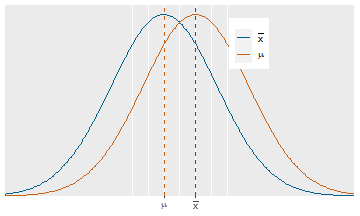
\includegraphics[width=.49\linewidth]{bookdownproj_files/figure-latex/double-1} 

}

\caption{Konstruierte Verteilung um $\bar{x}$}\label{fig:double}
\end{figure}

Dabei heißt der Bereich Konfidenzintervall (engl. \emph{confidence interval}), und seine Breite wird mit \(\textrm{KIB}\) abgekürzt. Die Wahrscheinlichkeit, dass wir mit unserer Schätzung \emph{außerhalb} des Konfidenzintervalls liegen wird mit \(\alpha\) gekennzeichnet. Ein 95\%-Konfidenzintervall hat also ein \(\alpha\) von 0,05 (s. \autoref{fig:konf}).

\begin{figure}[h]

{\centering 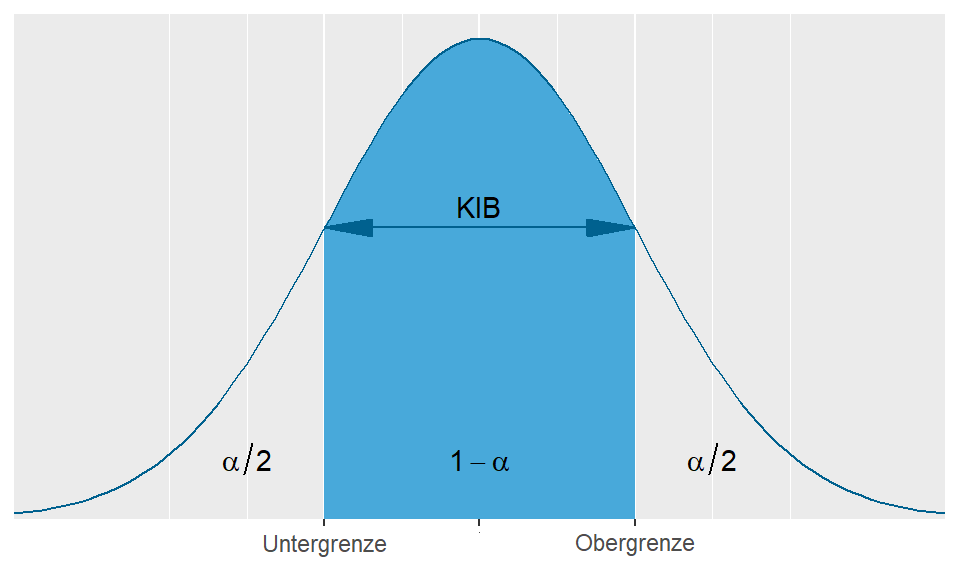
\includegraphics[width=.49\linewidth]{bookdownproj_files/figure-latex/konf-1} 

}

\caption{Konfidenzintervall}\label{fig:konf}
\end{figure}

\begin{table}

\caption{\label{tab:tab}Jahresniederschlag in Hessen}
\centering
\begin{tabular}[t]{rr}
\toprule
Jahr & Niederschlag (l/m²)\\
\midrule
2011 & 855,3\\
2012 & 839,5\\
2013 & 850,6\\
2014 & 873,1\\
2015 & 858,3\\
2016 & 857,1\\
2017 & 861,4\\
\bottomrule
\end{tabular}
\end{table}

Ein Beispiel soll dies verdeutlichen: Wir wissen, dass die jährliche Niederschlagsmenge in Hessen normalverteilt ist mit \(\sigma=10{,}23\). Wir haben die Messwerte in Tabelle 1 erhoben und möchten den Mittelwert (\(\mu\)) per Intervallschätzung angeben.

Zunächst errechnen wir den Mittelwert unserer empirischen Stichprobe:

\nopagebreak

\[\begin{aligned}
  \bar{x}&\approx856{,}47
\end{aligned}\]

Dann errechnen wir anhand \autoref{eq:sd} den Standardfehler der theoretischen Verteilung von \(\bar{x}\):

\nopagebreak

\[\begin{aligned}
\sigma_{\bar{x}}&=\frac{\sigma}{\sqrt{n}}\\[4pt]
           &\approx\frac{10{,}23}{\sqrt{7}}\approx3,86
\end{aligned}\]

\hypertarget{gesuchtes-alpha}{%
\subsubsection{\texorpdfstring{Gesuchtes \(\alpha\)}{Gesuchtes \textbackslash alpha}}\label{gesuchtes-alpha}}

Nun könnte eine Fragerichtung lauten: Wie groß ist die Wahrscheinlichkeit, dass der Mittelwert der Population \(\mu\) in einem Korridor von ± 5 l/m² um \(\bar{x}\) liegt?\footnote{Genau genommen ist das nicht ganz korrekt, ``denn tatsächlich kann der Parameter nur innerhalb oder außerhalb des gefundenen Bereichs liegen. Die Wahrscheinlichkeit, dass ein Parameter in einen bestimmten Bereich fällt, ist damit entweder 0 oder 1.'' (\protect\hyperlink{ref-bortz}{Bortz und Schuster 2010}: 93). Mathematisch korrekt müsste es heißen: ``Die Wahrscheinlichkeit, dass \(\bar{x}\) zu einer Population gehört, deren Parameter \(\mu\) in diesem Bereich liegt\ldots{}''}

Gesucht ist bei einer Konfidenzintervallbreite von \(\textit{KIB}=10\) also die Wahrscheinlichkeit:

\nopagebreak

\[1-\alpha\approx P(851{,}47 < \mu < 861{,}47)\]

Generalisierend lässt sich schreiben:

\nopagebreak

\[
1-\alpha=P(x_{\alpha/2} < \mu < x_{(1-\alpha/2)})
\]

\nopagebreak

\ldots wobei \(x_{\alpha/2}\) die Untergrenze darstellt und \(x_{(1-\alpha/2)}\) die Obergrenze.

In \(z\)-Werten ausgedrückt:

\nopagebreak

\[
1-\alpha=P(z_{\alpha/2} < z_{\mu} < z_{(1-\alpha/2)})
\]\{\#eq:konf\}

In Sitzung 3 haben wir bereits gelernt, wie diese Wahrscheinlichkeit berechnet werden kann. Im Folgenden wird der Rechenweg noch einmal am Beispiel dargelegt.

\hypertarget{die-umstuxe4ndliche-variante}{%
\paragraph{Die umständliche Variante}\label{die-umstuxe4ndliche-variante}}

Zunächst müssen wir die Intervallgrenzen in\(z\)-Werte umwandeln, um die Unter- bzw. Überschreitungswahrscheinlichkeiten ermitteln zu können. Die z-Transformation muss hier jedoch anhand des Standardfehlers \(\sigma_{\bar{x}}\) geschehen, da wir ja an der Stichprobenverteilung interessiert sind. Durch \(z\)-Transformation mit \(\bar{x}\) und dem Standardfehler \(\sigma_{\bar{x}}\) erhalten wir die standardisierten Intervallgrenzen.

Untergrenze:

\nopagebreak

\[\begin{aligned}
z_{\alpha/2} &= \frac{x_{\alpha/2}-\bar{x}}{\sigma_{\bar{x}}}\\[4pt]
&\approx\frac{851{,}47-856,47}{3,86}\approx-1,30
\end{aligned}\]

Obergrenze:

\nopagebreak

\[\begin{aligned}
z_{(1-\alpha/2)} &= \frac{x_{(1-\alpha/2)}-\bar{x}}{\sigma_{\bar{x}}}\\[4pt]
&\approx\frac{861{,}47-856,47}{3,86}\approx1,30
\end{aligned}\]

Es ist wenig überraschend, dass die \(z\)-transformierten Werte symmetrisch sind. Wir setzen in \autoref{eq:konf} ein:

\nopagebreak

\[
1-\alpha\approx P(-1{,}30 <z_{\mu} < 1{,}30)
\]

Dies lässt sich umformen in:

\nopagebreak

\[
1-\alpha\approx P(z_{\mu}<1{,}08) - P(z_{\mu}<-1{,}08) 
\]

Die jeweiligen Wahrscheinlichkeiten lassen sich in der Tabelle für \(p\)-Werte der Normalverteilung nachschauen (bzw. für den negativen \(z\)-Wert errechnen, s. Sitzung 3):

\nopagebreak

\[\begin{aligned}
1-\alpha&\approx 0,9032 - 0,0968\\[4pt]
&=0,8064
\end{aligned}\]

Die Wahrscheinlichkeit, dass \(\mu\) im Konfidenzintervalls 856,47 ± 5 l/m² liegt, beträgt also 80,64\%.

\hypertarget{die-schnelle-variante}{%
\paragraph{Die schnelle Variante}\label{die-schnelle-variante}}

Wir können den \(z\)-Wert für die Obergrenze des Konfidenzintervalls ganz einfach ausrechnen, weil wir wissen, dass die Obergrenze um 5 größer ist als \(\bar{x}\) und dass \(z_{\bar{x}}=0\):

\nopagebreak

\[\begin{aligned}
z_{(1-\alpha/2)}&=\frac{5}{\sigma_{\bar{x}}}\\[4pt]
&\approx\frac{5}{3,86}\\[4pt]
&\approx1{,}30
\end{aligned}\]

Oberhalb dieses Werts liegt bekanntermaßen der Anteil \(\frac{\alpha}{2}\), woraus sich mit Blick auf die Tabelle ergibt:

\nopagebreak

\[\begin{aligned}
\frac{\alpha}{2}&=1-0,9032\\[4pt]
\alpha&=0,1936
\end{aligned}\]

\hypertarget{gesuchtes-konfidenzintervall}{%
\subsubsection{Gesuchtes Konfidenzintervall}\label{gesuchtes-konfidenzintervall}}

Eine weitere Möglichkeit der Fragestellung lautet: In welchem Bereich liegt das arithmetische Mittel \(\mu\) mit einer Wahscheinlichkeit von 90\%?

Vorgegeben ist also \(\alpha=0{,}1\), und gesucht sind die Unter- und die Obergrenze des Konfidenzintervalls.

Wir setzen ein:

\nopagebreak

\[\begin{aligned}
1-\alpha&=P(z_{\alpha/2} < z_{\mu} < z_{(1-\alpha/2)})\\[4pt]
0{,}9 &= P(z_{5\%} < z_{\mu} < z_{95\%})
\end{aligned}\]

Die entsprechenden \(z\)-Werte der Intervallgrenzen lassen sich (in umgekehrter Suchrichtung) aus der Tabelle ablesen:

\nopagebreak

\[\begin{aligned}
z_{5\%}&\approx-1{,}64\\[4pt]
z_{95\%}&\approx 1{,}64
\end{aligned}\]

Durch umgekehrte z-Transformation -- auch hier weider mit \(\bar{x}\) und \(\sigma_{\bar{x}}\) -- ergeben sich die Intervallgrenzen.

Untergrenze:

\nopagebreak

\[\begin{aligned}
x_{5\%} &= z_{5\%} \cdot \sigma_{\bar{x}} + \bar{x}\\[4pt]
&\approx -1{,}64 \cdot 3,86 + 856{,}47\\[4pt]
&\approx 850,14\\[6pt]
\end{aligned}\]

Obergrenze:

\nopagebreak

\[\begin{aligned}
x_{95\%}&= z_{95\%} \cdot \sigma_{\bar{x}} + \bar{x}\\[4pt]
&\approx 1{,}64 \cdot 3,86 + 856{,}47\\[4pt]
&\approx 862,80
\end{aligned}\]

Auch hier gibt es wieder eine kleine Abkürzung: Aufgrund der Symmetrie unserer theoretischen Verteilung gilt für die Konfidenzintervallbreite generell:

\nopagebreak

\[
\frac{\mathit{KIB}}{2} = z_{(1-\alpha/2)} \cdot \sigma_{\bar{x}}
\]\{\#eq:kib\}

Wir setzen einfach unsere Werte ein:

\nopagebreak

\[\begin{aligned}
\frac{\mathit{KIB}}{2} &= z_{95\%} \cdot s_{\bar{x}}\\[4pt]
&\approx1{,}64 \cdot 3,86\\[4pt]
&\approx 6,33
\end{aligned}\]

Die Intervallgrenzen ergeben sich dann trivial aus \(\bar{x} \pm \frac{\mathit{KIB}}{2}\).

\hypertarget{gesuchtes-n}{%
\subsubsection{\texorpdfstring{Gesuchtes \(n\)}{Gesuchtes n}}\label{gesuchtes-n}}

Eine letzte Fragerichtung lautet: Wie viele Messwerte müssten vorliegen, um den durchschnittlichen Niederschlag mit einem Konfidenzniveau von 99\% und einer Genauigkeit von ± 5 l/m² schätzen zu können?

Gegeben sind also das Konfidenzintervall und \(\alpha=0{,}01\), gesucht wird \(n\). Wir wissen, dass die Stichprobengröße \(n\) den Standardfehler \(\sigma_{\bar{x}}\) bestimmt. Also benutzen wir zunächst \autoref{eq:kib} und formen um:

\nopagebreak

\[\begin{aligned}
\frac{\mathit{KIB}}{2} &= z_{(1-\alpha/2)} \cdot \sigma_{\bar{x}}\\[4pt]
\sigma_{\bar{x}} &= \frac{\mathit{KIB}}{2\cdot z_{(1-\alpha/2)}} 
\end{aligned}\]

Durch Einsetzen und mit Blick auf die Tabelle erhalten wir:

\nopagebreak

\[\begin{aligned}
\sigma_{\bar{x}} &= \frac{10}{2\cdot z_{99{,}5\%}}\\[4pt]
 &\approx \frac{10}{2\cdot 2{,}58}\\[4pt]
 &\approx 1{,}94
\end{aligned}\]

Dieser Standardfehler \(\sigma_{\bar{x}}\approx1{,}94\) würde unseren Anforderungen genügen. Welches \(n\) ist nötig, um diesen Standardfehler zu erreichen? Wir formen \autoref{eq:sd} um\ldots{}

\nopagebreak

\[\begin{aligned}
\sigma_{\bar{x}} &= \frac{\sigma}{\sqrt{n}}\\[4pt]
               n &= \Big(\frac{\sigma}{\sigma_{\bar{x}}}\Big)^2
\end{aligned}\]

\ldots und setzen den angestrebten Standardfehler sowie die Standardabweichung der Population (\(\sigma=10{,}23\)) ein:

\nopagebreak

\[\begin{aligned}
n&=\Big(\frac{\sigma}{\sigma_{\bar{x}}}\Big)^2\\[4pt]
n&\approx\bigg(\frac{10{,}23}{1{,}94}\bigg)^2\\[4pt]
&\approx27{,}80
\end{aligned}\]

Wir müssten also 28 Stichproben vorliegen haben.

\hypertarget{aufgaben-3}{%
\subsection{Aufgaben}\label{aufgaben-3}}

Die folgenden Aufgaben sind zur eigenständigen Überprüfung Ihrer Lernleistung gedacht (als Vor- oder Nachbereitung der Vorlesung, oder als Klausurübung) und nicht etwa als Hausaufgabe.

\hypertarget{aufgabe-1-3}{%
\subsubsection{Aufgabe 1}\label{aufgabe-1-3}}

Eine Messreihe habe die Werte:
\texttt{165\ 173\ 155\ 179\ 158\ 142}

\begin{enumerate}
\def\labelenumi{\alph{enumi})}
\tightlist
\item
  Führen Sie eine Punktschätzung für \(\mu\) und \(\sigma\) der Grundgesamtheit durch.
\item
  Welcher Standardfehler für \(\bar{x}\) ist zu erwarten?
\end{enumerate}

\hypertarget{aufgabe-2-3}{%
\subsubsection{Aufgabe 2}\label{aufgabe-2-3}}

Die Sonnenstunden auf einer Ferieninsel (pro Tag, im Jahresdurschnitt) sind annähernd normalverteilt mit einer Standardabweichung von vier Minuten. Der Mittelwert \(\mu\) ist unbekannt, es liegen neun Messwerte vor.

\begin{enumerate}
\def\labelenumi{\alph{enumi})}
\tightlist
\item
  Welcher Standardfehler für \(\bar{x}\) ist zu erwarten?
\item
  Welche Konfidenzintervallbreite korrespondiert mit einem Konfidenzniveau von 95\%?
\item
  Mit welchem Konfidenzniveau lässt sich \(\mu\) ``auf die Minute genau'' (± 30 Sekunden) schätzen?
\item
  Welche Stichprobengröße ist nötig um den Mittelwert mit einer Konfidenzintervallbreite von zwei Minuten und -niveau von 90\% zu schätzen?
\end{enumerate}

\hypertarget{aufgabe-3-1}{%
\subsubsection{Aufgabe 3}\label{aufgabe-3-1}}

Sie intressieren sich für das Durchschnittseinkommen (in EUR) der Haushalte eines Stadtteils. Die Varianz ist mit \(\sigma^2=4096\) bekannt. Eine Zufallsstichprobe von 40 befragten Haushalten weist einen Mittelwert von \(\bar{x}=2650\) auf.

\begin{enumerate}
\def\labelenumi{\alph{enumi})}
\tightlist
\item
  Wie lautet das 90\%-Konfidenzintervall?
\item
  Mit welcher Wahrscheinlichkeit liegt das Durchschnittseinkommen zwischen 2640 und 2660 EUR?
\end{enumerate}

\hypertarget{tipps-zur-vertiefung-3}{%
\subsection{Tipps zur Vertiefung}\label{tipps-zur-vertiefung-3}}

\begin{itemize}
\tightlist
\item
  YouTube-Kanal ``Kurzes Tutorium Statistik'': \href{https://www.youtube.com/watch?v=DdwTa28W4Os}{Intervallschätzungen - Konfidenzintervalle}
\item
  Kapitel 8 in \protect\hyperlink{ref-klemm}{Klemm} (\protect\hyperlink{ref-klemm}{2002})
\item
  Kapitel 6.2--6.4 in \protect\hyperlink{ref-bortz}{Bortz und Schuster} (\protect\hyperlink{ref-bortz}{2010})
\item
  Kapitel 5.3.1 in \protect\hyperlink{ref-bahrenberg}{Bahrenberg, Giese und Nipper} (\protect\hyperlink{ref-bahrenberg}{2010})
\end{itemize}

\hypertarget{quellen-3}{%
\subsection{Quellen}\label{quellen-3}}

\hypertarget{grundlagen-der-teststatistik}{%
\section{Grundlagen der Teststatistik}\label{grundlagen-der-teststatistik}}

\hypertarget{lernziele-dieser-sitzung-4}{%
\subsection{Lernziele dieser Sitzung}\label{lernziele-dieser-sitzung-4}}

Sie können\ldots{}

\begin{itemize}
\tightlist
\item
  Hypothesen formulieren.
\item
  einen \(z\)-Test durchführen.
\item
  einen 1-Stichproben-\(t\)-Test durchführen.
\end{itemize}

\hypertarget{statistische-tests}{%
\subsection{Statistische Tests}\label{statistische-tests}}

Gemeinsam mit der Schätzstatistik bildet die Test- bzw. Prüfstatistik jenen Teil statistischer Verfahren, die ausgehend von einer Stichprobenverteilung Rückschlüsse auf die Beschaffenheit von Grundgesamtheiten anstreben (schließende Statistik).

Dabei haben Schätz- und Teststatistik jedoch grundlegend verschiedene Vorgehensweisen. Wie in Sitzung 4 besprochen ermöglicht die Schätzstatistik die Angabe statistischer Parameter einer Grundgesamtheit anhand von Stichprobenwerten, und unter Angabe von Wahrscheinlichkeiten.

Ziel statistischer Tests hingegen ist es, mit Hilfe von Stichproben Hypothesen (also Vermutungen) über die Grundgesamtheit zu prüfen. Geprüft wird dabei ein empirischer Sachverhalt gegen die Zufälligkeit seiner Realisierung. Ein statistischer Test fragt, ab welcher Größenordnung ein Stichprobenergebnis nicht mehr als zufällig, sondern als \emph{signifikant} anzusehen ist.

Dabei folgt die grundsätzliche Vorgehensweise von (hier behandelten) statistischen Tests immer diesem Schema:

\begin{enumerate}
\def\labelenumi{\arabic{enumi}.}
\tightlist
\item
  Test wählen und Voraussetzungen prüfen
\item
  Hypothesen formulieren
\item
  Signifikanzniveau entscheiden
\item
  Ablehnungsbereich bestimmen
\item
  Prüfgröße berechnen
\item
  Ergebnis interpretieren
\end{enumerate}

Die einzelnen Schritte werden im Folgenden direkt anhand des \(z\)-Tests besprochen.

\hypertarget{z-test}{%
\subsection{\texorpdfstring{\(z\)-Test}{z-Test}}\label{z-test}}

Die mathematischen Grundlagen des \(z\)-Tests leiten sich direkt aus der in Sitzung 4 besprochenen Stichprobenverteilung für \(\bar{x}\) ab.

Ein illustrierendes Beispiel: Wir wissen, dass die Anzahl der täglichen Besucher*innen einer Eissporthalle annähernd normalverteilt ist, und zwar mit dem arithmetischen Mittel \(\mu=94{,}2\) und der Standardabweichung \(\sigma=11{,}8\). Wir vermuten, dass die Anzahl der Besucher*innen an bewölkten Tagen größer ist, weil an sonnigen Tagen andere Freizeitbeschäftigungen attraktiver sind.

An fünf zufälligen bewölkten Tagen zählen wir die Besucher*innen und kommen auf einen Mittelwert der Stichprobe von \(\bar{x} = 103{,}0\).

Dieser Wert ist höher als das arithmetische Mittel der Grundgesamtheit (\(\mu\)). Aber heißt das auch, dass unsere Vermutung stimmt? Wir wissen aus Sitzung 4, dass die Stichprobenverteilung einem Standardfehler (\(\sigma_{\bar{x}}\)) unterliegt (s. \autoref{fig:eis}).

Ist das Ergebnis also nur zufällig zustande gekommen, oder liegt ein \emph{statistisch signifikantes} Ergebnis vor? Mit anderen Worten: Ist die Stichprobe überhaupt der Verteilung \(x_0\) um \(\mu_0\) entnommen, oder gibt es eine \emph{andere} Verteilung (\(x\) um ein anderes \(\mu\)) für bewölkte Tage, denen unser Stichprobenmittelwert \(\bar{x}\) entstammt? Genau diese Art von Frage versuchen statistische Tests zu beantworten.

\begin{figure}[h]

{\centering 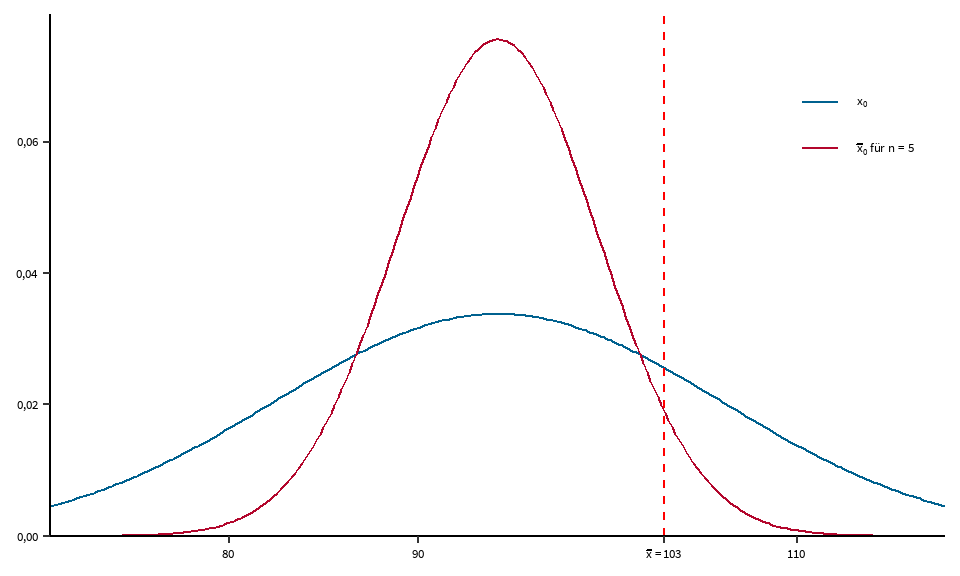
\includegraphics[width=.49\linewidth]{bookdownproj_files/figure-latex/eis-1} 

}

\caption{Theoretische Stichprobenverteilung (unter Annahme der Nullhypothese)}\label{fig:eis}
\end{figure}

\hypertarget{test-wuxe4hlen-und-voraussetzungen-pruxfcfen}{%
\subsubsection{Test wählen und Voraussetzungen prüfen}\label{test-wuxe4hlen-und-voraussetzungen-pruxfcfen}}

Je nachdem, was überprüft werden soll, was über die Grundgesamtheit bekannt ist und wie die Stichprobe beschaffen ist, müssen verschiedene Testverfahren angewendet werden.

Statistische Tests unterscheiden sich zunächst in Bezug auf ihre Prüfgröße (und sind auch nach ihrer Prüfgröße benannt). Wir werden zunächst den \(z\)-Test kennenlernen, der mit dem (uns seit Sitzung 3 bekannten) \(z\)-Wert als Prüfgröße arbeitet.

Der \(z\)-Test hat zum Ziel, den Mittelwert einer Stichprobe mit den zu erwartenden Werten bei einer bekannten Verteilung zu vergleichen.

Um den \(z\)-Test anwenden zu können, müssen also folgende Voraussetzungen gegeben sein:
- Das Ziel der Untersuchung ist es, eine signifikante Abweichung des Mittelwerts festzustellen.
- Das arithmetische Mittel \(\mu\) und die Standardabweichung \(\sigma\) der (ursprünglichen) Grundgesamtheit müssen bekannt sein.
- Der Test muss anhand einer reinen Zufallsstichprobe erfolgen.
- Die Stichprobenverteilung muss (annähernd) normalverteilt sein, das heißt:
- \emph{entweder} die Grundgesamtheit ist (annähernd) normalverteilt,
- \emph{oder} die Stichprobe hat die Größe \(n\geq30\).

\hypertarget{beispiel}{%
\paragraph{Beispiel}\label{beispiel}}

In unserem Beispiel (Besucherzahlen der Eissporthalle) sind diese Voraussetzungen gegeben. Wir können und wollen also einen \(z\)-Test durchführen.

\hypertarget{hypothesen-formulieren}{%
\subsubsection{Hypothesen formulieren}\label{hypothesen-formulieren}}

Es müssen immer zwei Hypothesen formuliert werden: die Nullhypothese und die Alternativhypothese. Die Nullhypothese geht immer davon aus, dass es keine Abweichung gibt, die Alternativhypothese formuliert eine Abweichung.

Dabei werden zwei Verteilungen konstruiert: Die bekannte Grundgesamtheit (in unserem Beispiel: Besucherzahlen insgesamt) \(x_0\) mit Mittelwert \(\mu_0\) und eine neue Verteilung (Besucherzahlen an bewölkten Tagen) \(x\) mit Mittelwert \(\mu\).

Die Hypothesen sind theoriegeleitet (formulieren also eine begründete Vermutung) und stehen stets am Anfang der statistischen Untersuchung. Es ist unzulässig, sie im Nachhinein anzupassen.

\hypertarget{nullhypothese}{%
\paragraph{Nullhypothese}\label{nullhypothese}}

Die Nullhypothese (engl. \emph{null hypothesis}) geht immer davon aus, das die forscherische Vermutung nicht stimmt. Im \(z\)-Test besagt die Nullhypothese, dass es zwischen dem Mittelwert \(\mu_0\) und dem Mittelwert \(\mu\) keinen Unterschied gibt. Generell heißt die Nullhypothese:

\[
H_0 : \mu = \mu_0
\]\{\#eq: h0\}

\hypertarget{alternativhypothese}{%
\paragraph{Alternativhypothese}\label{alternativhypothese}}

Die Alternativhypothese (engl. \emph{alternative hypothesis}) stellt die Vermutung dar, die überprüft werden soll. Dabei gibt es zwei unterschiedliche Möglichkeiten: ungerichtete und gerichtete Alternativhypothesen.

\hypertarget{ungerichtete-alternativhypothese}{%
\subparagraph{Ungerichtete Alternativhypothese}\label{ungerichtete-alternativhypothese}}

Die ungerichtete Alternativhypothese besagt nur, \emph{dass} es einen Unterschied zwischen \(\mu\) und \(\mu_0\) gibt, aber nicht in welche Richtung (größer oder kleiner). Sie lautet daher:

\[
H_1 : \mu \neq \mu_0
\]\{\#eq:h1u\}

\hypertarget{gerichtete-alternativhypothese}{%
\subparagraph{Gerichtete Alternativhypothese}\label{gerichtete-alternativhypothese}}

Die gerichtete Alternativhyptothese gibt eine Richtung des vermuteten Unterschieds (nach oben oder unten) vor. Sie lautet entweder:

\[
H_1 : \mu < \mu_0 \quad \textrm{(abwärts gerichtet)}
\]\{\#eq:h1l\}

oder:

\[
H_1 : \mu > \mu_0 \quad \textrm{(aufwärts gerichtet)}
\]\{\#eq:h1g\}

\hypertarget{beispiel-1}{%
\paragraph{Beispiel}\label{beispiel-1}}

In unserem Beispiel geben wir eine Richtung vor, denn wir vermuten ja, dass die Besucherzahlen an bewölkten Tagen \emph{höher} sind. Wir schreiben also:

\[\begin{aligned}
H_0: \mu = 94{,}2\\[4pt]
H_1: \mu>94{,}2
\end{aligned}\]

\hypertarget{signifikanzniveau-entscheiden}{%
\subsubsection{Signifikanzniveau entscheiden}\label{signifikanzniveau-entscheiden}}

Das Signifikanzniveau \(\alpha\) (engl. \emph{significance level}) entscheidet, wie \emph{unwahrscheinlich} eine Prüfgröße unter Annahme der Nullhypothese sein muss, damit wir die Nullhypothese ablehnen können (und damit unsere Annahme bestätigen).

Übliche Werte für das Signifikanzniveau sind \(\alpha=0{,}05\) oder \(\alpha=0{,}01\).

Für die Wahl des Signifikanzniveaus ist jeweils der Kontext entscheidend: Wenn die irrtümliche Bestätigung der forscherischen Annahme gravierende Auswirkungen hat, möchte man das Signifikanzniveau besonders niedrig wählen um diese Art von Fehler auszuschließen.

Auch das Signifikanzniveau muss vor der statistischen Erhebung formuliert werden, und es ist unzulässig, es im Nachhinein an das Ergebnis anzupassen.

\hypertarget{beispiel-2}{%
\paragraph{Beispiel}\label{beispiel-2}}

Ein Irrtum in der statistischen Signifikanz der Besucherzahl hat vermutlich keine gravierenden Folgen. Wir legen das Signifikanzniveau auf \(\alpha=0{,}05\) fest.

\hypertarget{ablehnungsbereich-bestimmen}{%
\subsubsection{Ablehnungsbereich bestimmen}\label{ablehnungsbereich-bestimmen}}

Zusammen mit der (Un-)Gerichtetheit der Alternativhypothese bestimmt das Signifikanzniveau \(\alpha\) den \emph{Ablehnungsbereich} -- also den Bereich für die zu errechnende Prüfgröße \(z\), in dem die Nullhypothese abgelehnt würde.

Der Ablehnungsbereich für die ungerichtete Alternativhypothese ist \(\frac{\alpha}{2}\) auf beiden Seiten (s. \autoref{fig:ablung}). Die kritischen Werte sind dann die Schwellen des Ablehnungsbereich auf beiden Seiten:

\[
z \leq z_{\alpha/2} \quad \textrm{und} \quad z \geq z_{(1-\alpha/2)} \quad \textrm{für} \quad H_1: \mu \neq \mu_0
\]\{\#eq: kritneq\}

\begin{figure}[h]

{\centering 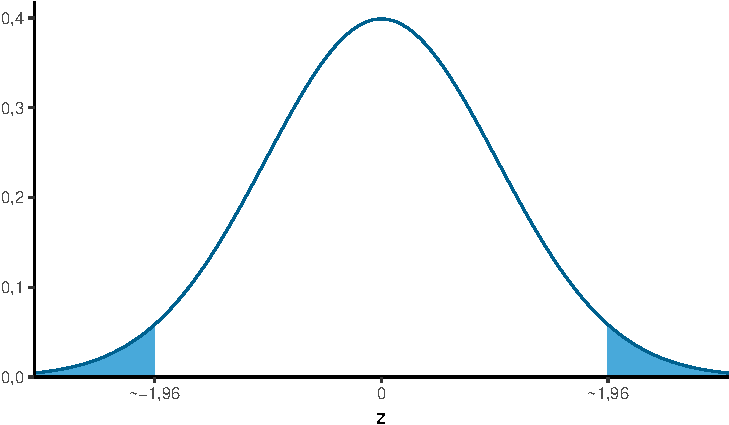
\includegraphics[width=.49\linewidth]{bookdownproj_files/figure-latex/ablung-1} 

}

\caption{Kritische Werte für $z$ bei ungerichteter Alternativhypothese und $\alpha=0{,}05$}\label{fig:ablung}
\end{figure}

Bei den gerichteten Alternativhypothesen ist der Ablehnungsbereich jeweils nur auf einer Seite (s. Abbildungen \ref{fig:ablger1} und \ref{fig:ablger2}). Die kritischen Werte ergeben sich aus:

\[
z \leq z_{\alpha} \quad \textrm{für} \quad H_1: \mu < \mu_0
\]\{\#eq: kritless\}
\[
z \geq z_{(1-\alpha)} \quad \textrm{für} \quad H_1: \mu > \mu_0
\]\{\#eq: kritless\}

\begin{figure}[h]

{\centering 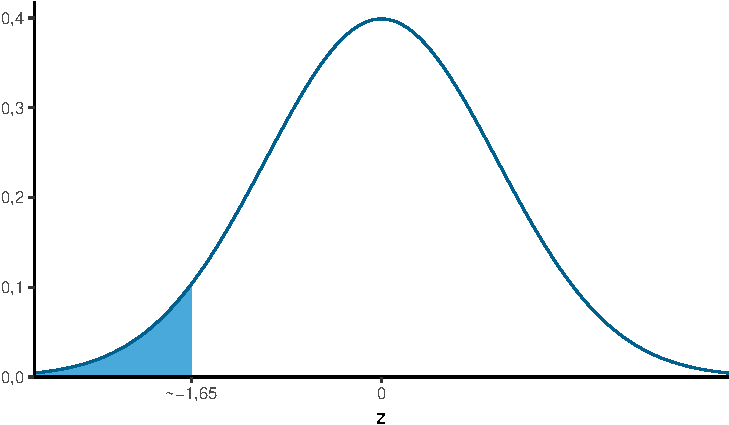
\includegraphics[width=.49\linewidth]{bookdownproj_files/figure-latex/ablger1-1} 

}

\caption{Kritischer Wert für $z$ bei gerichteter Alternativhypothese nach unten und $\alpha=0{,}05$}\label{fig:ablger1}
\end{figure}

\begin{figure}[h]

{\centering 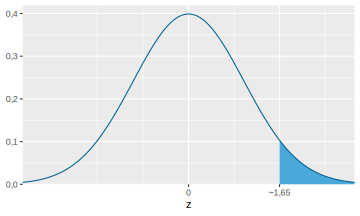
\includegraphics[width=.49\linewidth]{bookdownproj_files/figure-latex/ablger2-1} 

}

\caption{Kritischer Wert für $z$ bei gerichteter Alternativhypothese nach oben und $\alpha=0{,}05$}\label{fig:ablger2}
\end{figure}

\hypertarget{beispiel-3}\approx 1{,}65
\]

Der Mittelwert unserer Stichprobe fällt höher aus als \(\mu\). Aber übersteigt er auch den kritischen Wert (und ist damit statistisch signifikant)?

\hypertarget{pruxfcfgruxf6uxdfe-berechnen}{%
\subsubsection{Prüfgröße berechnen}\label{pruxfcfgruxf6uxdfe-berechnen}}

Für den \(z\)-Test ist die Prüfgröße der \(z\)-Wert der Stichprobe, und zwar standardisiert in Bezug auf \(\mu_0\) und den Standardfehler (\(\sigma_{\bar{x}}\)):

\[
z=\frac{\bar{x}-\mu_0}{\sigma_{\bar{x}}}
\]\{\#eq:trans\}

Wie wir bereits wissen, ergibt sich der Standardfehler (\(\sigma_{\bar{x}}\)) wiederum aus der Stichprobengröße (\(n\)) und der Standardabweichung der Grundgesamtheit (\(\sigma\)):

\[
\sigma_{\bar{x}}=\frac{\sigma}{\sqrt{n}}
\]\{\#eq:serr\}

Durch einsetzen ergibt sich die generelle Formel für die Prüfgröße des \(z\)-Tests:

\[
z=\sqrt{n}\cdot\frac{\bar{x}-\mu_0}{\sigma}
\]\{\#eq:z\}

Das grundsätzliche Schema dieser Formel werden wir in anderen Tests wiedererkennen.

\hypertarget{beispiel-4}{%
\paragraph{Beispiel}\label{beispiel-4}}

An dieser Stelle (also \emph{nachdem} wir uns für einen Test und ein Signifikanzniveau entschieden und den kritischen Wert berechnet haben) dürften wir streng genommen erst die Stichprobe erheben.

Diese ergibt bei \(n=5\) den Mittelwert \(\bar{x}=103{,}0\). Die Verteilung \(x_0\) (also unter Annahme der Nullhypothese) hatte die Kennwerte \(\mu_0=94{,}2\) und \(\sigma=11{,}8\).

Wir setzen ein in die Formel aus \autoref{eq:z}:

\[\begin{aligned}
z&=\sqrt{n}\cdot\frac{\bar{x}-\mu_0}{\sigma}\\[4pt]
 &\approx\sqrt{5}\cdot\frac{103{,}0-94{,}2}{11{,}8}\\[4pt]
 &\approx1{,}67
\end{aligned}\]

\hypertarget{ergebnis-inerpretieren}{%
\subsubsection{Ergebnis inerpretieren}\label{ergebnis-inerpretieren}}

Je nachdem, ob die Prüfgröße in den Ablehnungsbereich fällt (ob der kritische Wert also unter- bzw. überschritten wird), können wir die Nullhypothese ablehnen (und damit unsere Alternativhypothese bestätigen) oder nicht.

Eine Ablehnung der Nullhypothese bedeutet, dass wir ein \emph{statistisch signifikantes Ergebnis zugunsten unserer Vermutung} vorliegen haben.

Diese Art von Ergebnis wird oft falsch interpretiert. Bei einem Signifikanzniveau von \(\alpha=0{,}01\) heißt das zum Beispiel, dass die beobachteten Werte nur mit 1\% Wahrscheinlichkeit vorkommen, wenn unsere Vermutung \emph{nicht} stimmt. Wichtig dabei: Das ist etwas ganz anderes als zu behaupten, dass unsere Vermutung zu 99\% stimme. Über die Wahrscheinlichkeit, dass eine Hypothese stimmt (oder nicht) können wir mit den Methoden der klassischen Statistik keine Aussage machen!

\hypertarget{beispiel-5}{%
\paragraph{Beispiel}\label{beispiel-5}}

In unserem Beispiel liegt der \(z\)-Wert knapp über dem kritischen Wert von 1,65. Wir können also die Nullhypothese ablehnen und unsere Alternativhypothese annehmen. Unsere statistische Untersuchung hat gezeigt, dass die Eissporthalle an bewölkten Tagen besser besucht ist als an sonnigen (und zwar mit Signifikanzniveau \(\alpha=0,05\)).

Gut, dass wir eine gerichtete Alternativhypothese aufgestellt haben. Hätten wir nur vermutet, dass sich die Besucherzahlen je nach Wetter unterscheiden (ohne Angabe einer Richtung), dann wäre der kritische Wert nicht erreicht worden und wir hätten die Nullhypothese beibehalten müssen. Hinterher die Hypothesen anzupassen ist natürlich nicht zulässig!

\begin{rtip}
R hat in der Grundversion keinen dezidierten Befehl für einen $z$-Test. Mit der Funktion {\tt qnorm()} können kritische Werte jedoch einfach bestimmt werden.
\end{rtip}

\hypertarget{die-t-verteilung}{%
\subsection{\texorpdfstring{Die \(t\)-Verteilung}{Die t-Verteilung}}\label{die-t-verteilung}}

Wenn die Standardabweichung \(\sigma\) eines Merkmals in der Grundgesamtheit \emph{unbekannt} ist, kann sie durch die Standardabweichung \(s\) der Stichprobe geschätzt werden (s. Sitzung 4). Dann ist die Stichprobenverteilung für \(\bar{x}\) jedoch nicht mehr normalverteilt, sondern sie folgt einer \(t\)-Verteilung.

Im Gegensatz zur Standardnormalverteilung (die wir für den \(z\)-Test benutzen) gibt es aber nicht nur eine \(t\)-Verteilung, sondern die Form der \(t\)-Verteilung hängt von so genannten Freiheitsgraden (engl. \emph{degrees of freedom}) ab. Mit steigender Zahl der Freiheitsgrade nähert sich die \(t\)-Verteilung einer Standardnormalverteilung an (s. \autoref{fig:tdf}).

\begin{figure}[h]

{\centering 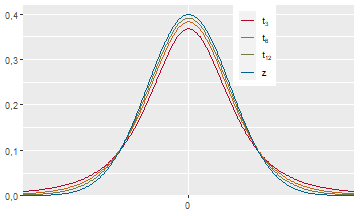
\includegraphics[width=.49\linewidth]{bookdownproj_files/figure-latex/tdf-1} 

}

\caption{$t$-Verteilungen mit verschiedenen Freiheitsgraden}\label{fig:tdf}
\end{figure}

\hypertarget{freiheitsgrade}{%
\subsubsection{Freiheitsgrade}\label{freiheitsgrade}}

In Anlehnung an \protect\hyperlink{ref-bortz}{Bortz und Schuster} (\protect\hyperlink{ref-bortz}{2010}) kürzen wir Freiheitsgrade mit \(\mathit{df}\) ab. Dort findet sich auch eine brauchbare Erklärung dieses Phänomens:

\begin{quote}
„Die Freiheitsgrade, welche mit einem Kennwert verbunden sind, entsprechen der Anzahl der Werte, die bei seiner Berechnung frei variieren können. Der Mittelwert \(\bar{x}\) besitzt beispielsweise \(n\) Freiheitsgrade, weil es keinerlei Bedingung gibt, der die \(n\) Werte genügen müssen. Dies ist für die Varianz \(s^2=\mathit{QS}/(n-1)\) nicht der Fall. Nur \(n-1\) Abweichungen, welche in die Berechnung der Quadratsumme \(\mathit{QS}=\sum_i(x_i-\bar{x})^2\) eingehen, können frei variieren. {[}D{]}ie Summe der Abweichungen von ihrem Mittelwert {[}ist{]} null, d.h. \(\sum_i(x_i-\bar{x})=0\). Von \(n\) Abweichungen können deshalb nur \(n - 1\) frei variieren. Ergeben sich beispielsweise bei einer Stichprobe aus drei Werten die Abweichungen \(x_1 - \bar{x} = -4\) und \(x_2 - \bar{x} = 0\), muss zwangsläufig \(x_3 -\bar{x} = 4\) sein, damit die Summe aller Abweichungen null ergibt. Bei der Varianzberechnung ist eine der \(n\) Abweichungen festgelegt, d.h. die Varianz hat nur \(n - 1\) Freiheitsgrade. Man schreibt die Stichprobenvarianz deshalb gelegentlich auch als \(s^2 = \mathit{QS}/\mathit{df}\). Da die Varianz mit \(n - 1\) Freiheitsgraden verbunden ist, gilt dies auch für die Standardabweichung \(s\).`` (\protect\hyperlink{ref-bortz}{Bortz und Schuster 2010}: 121)
\end{quote}

\hypertarget{stichproben-t-test}{%
\subsection{\texorpdfstring{1-Stichproben-\(t\)-Test}{1-Stichproben-t-Test}}\label{stichproben-t-test}}

Der 1-Stichproben-\(t\)-Test vergleicht (wie der \(z\)-Test) die Werte einer Stichprobe mit der Grundgesamtheit. Das Vorgehen ist dabei analog zum \(z\)-Test, mit dem einzigen Unterschied, dass eine \(t\)-Verteilung mit \((n-1)\) Freiheitsgraden herangezogen wird.

Wir besprechen den 1-Stichproben-\(t\)-Test direkt an einem Beispiel:

Beim Frankfurter Amt für Wohnungswesen betrage die durchschnittliche Bearbeitungsdauer von Anträgen auf Wohngeld 30,2 Tage und sei normalverteilt. Wir vermuten, dass die Bearbeitungszeit zu Anfang des Wintersemesters höher ist als im Jahresdurchschnitt und planen eine zufällige Stichprobe von 12 Anträgen mit Einreichungsdatum im Oktober.

\hypertarget{test-wuxe4hlen-und-voraussetzungen-pruxfcfen-1}{%
\subsubsection{Test wählen und Voraussetzungen prüfen}\label{test-wuxe4hlen-und-voraussetzungen-pruxfcfen-1}}

Um den 1-Stichproben-\(t\)-Test durzuführen müssen folgende Voraussetzungen erfüllt sein:

\begin{itemize}
\tightlist
\item
  Das Ziel der Untersuchung ist es, eine statistisch signifikante Abweichung des Mittelwerts einer Stichprobe im Vergleich zu einer Grundgesamtheit festzustellen.
\item
  Das zu untersuchende Merkmal ist in der Grundgesamtheit normalverteilt.
\item
  Das arithmetische Mittel (\(\mu\)) des Merkmals in der Grundgesamtheit ist bekannt. (Im Gegensatz zum \(z\)-Test ist \(\sigma\) hier unbekannt!)
\item
  Der Test erfolgt anhand einer reinen Zufallsstichprobe.
\end{itemize}

\hypertarget{beispiel-6}{%
\paragraph{Beispiel}\label{beispiel-6}}

In unserem Beispiel (Bearbeitungszeit Wohngeldanträge) sind diese Bedingungen erfüllt und wir können einen 1-Stichproben-\(t\)-Test durchführen.

\hypertarget{hypothesen-formulieren-1}{%
\subsubsection{Hypothesen formulieren}\label{hypothesen-formulieren-1}}

Die Hypothesen werden genauso wie beim \(z\)-Test formuliert:

\hypertarget{nullhypothese-1}{%
\paragraph{Nullhypothese}\label{nullhypothese-1}}

\[
H_0 : \mu = \mu_0
\]\{\#eq: h0\}

\hypertarget{alternativhypothese-1}{%
\paragraph{Alternativhypothese}\label{alternativhypothese-1}}

\[
H_1 : \mu \neq \mu_0 \quad \textrm{(ungerichtet)}
\]\{\#eq:h1u\}

oder

\[
H_1 : \mu < \mu_0 \quad \textrm{(abwärts gerichtet)}
\]\{\#eq:h1l\}

oder

\[
H_1 : \mu > \mu_0 \quad \textrm{(aufwärts gerichtet)}
\]\{\#eq:h1g\}

\hypertarget{beispiel-7}{%
\paragraph{Beispiel}\label{beispiel-7}}

In unserem Beispiel geben wir eine Richtung vor, denn wir vermuten ja, dass die Bearbeitungsdauer zu Semesteranfang \emph{höher} ist. Wir schreiben also:

\[\begin{aligned}
H_0: \mu = 30{,}2\\
H_1: \mu>30{,}2
\end{aligned}\]

\hypertarget{signifikanzniveau-entscheiden-1}{%
\subsubsection{Signifikanzniveau entscheiden}\label{signifikanzniveau-entscheiden-1}}

Wie beim \(z\)-Test entscheidet das Signifikanzniveau \(\alpha\), wie \emph{unwahrscheinlich} eine Prüfgröße unter Annahme der Nullhypothese sein muss, damit wir die Nullhypothese ablehnen können (und damit unsere Annahme bestätigen).

Übliche Werte für das Signifikanzniveau sind auch beim \(t\)-Test \(\alpha=0{,}05\) oder \(\alpha=0{,}01\).

\hypertarget{beispiel-8}{%
\paragraph{Beispiel}\label{beispiel-8}}

Ein Irrtum zugunsten der Alternativhypothese hat bei unserer Untersuchung keine gravierenden Folgen. Angenommen, wir wollen uns in der Analyse trotzdem ganz sicher sein. Dann entscheiden wir uns für das Signifikanzniveau \(\alpha=0{,}01\).

\hypertarget{ablehnungsbereich-bestimmen-1}{%
\subsubsection{Ablehnungsbereich bestimmen}\label{ablehnungsbereich-bestimmen-1}}

Genau wie beim \(z\)-Test bestimmt das Signifikanzniveau \(\alpha\) den \emph{Ablehnungsbereich} -- also den Bereich für die zu errechnende Prüfgröße \(t\), in dem die Nullhypothese abgelehnt würde.

Der Ablehnungsbereich für die ungerichtete Alternativhypothese ist \(\frac{\alpha}{2}\) auf beiden Seiten. Die kritischen Werte sind dann die Schwellen des Ablehnungsbereich auf beiden Seiten:

\[
t \leq t_{\mathit{df};\alpha/2} \quad \textrm{und} \quad t \geq t_{\mathit{df};(1-\alpha/2)} \quad \textrm{für} \quad H_1: \mu \neq \mu_0
\]\{\#eq: kritneq\}

Bei den gerichteten Alternativhypothesen ist der Ablehnungsbereich jeweils nur auf einer Seite. Die kritischen Werte ergeben sich aus:

\[
t \leq t_{\mathit{df};\alpha} \quad \textrm{für} \quad H_1: \mu < \mu_0
\]\{\#eq: kritless\}
\[
t \geq t_{\mathit{df};(1-\alpha)} \quad \textrm{für} \quad H_1: \mu > \mu_0
\]\{\#eq: kritless\}

Die kritischen Werte für \(t\) bei gegebenem Freiheitsgrad \((n-1)\) und Flächenabschnitt lassen sich aus der Tabelle im Anhang ablesen. Dabei ist zu beachten, dass aufgrund der Symmetrie die Werte für Flächenanteile unter 50\% nicht in der Tabelle verzeichnet sind. Es gilt die Formel:

\[
P(-t_\mathit{df})=1-P(t_\mathit{df})
\]\{\#eq:negt\}

So ist zum Beispiel der Wert für \(t_{5;1\%}=-t_{5;99\%}=-3{,}365\).

\hypertarget{beispiel-9}{%
\paragraph{Beispiel}\label{beispiel-9}}

In unserem Beispiel haben wir eine gerichtete Alternativhypothese nach oben und ein Signifikanzniveau von \(\alpha=0{,}01\) verwendet. Wir haben uns zudem für eine Stichprobengröße von \(n=12\) entschieden, woraus der Freiheitsgrad \(\mathit{df}=n-1=11\) resultiert.

Der kritische Wert (bei dessen Überschreitung wir die Nullhypothese ablehnen und unsere Vermutung bestätigt sehen) lautet also:

\[\begin{aligned}
t &\geq t_{\mathit{df};(1-\alpha)}\\[4pt]
t &\geq t_{11;99\%}\\[4pt]
t &\geq 2,718
\end{aligned}\]

Graphisch ist der Ablehnungsbereich für unser Beispiel in \autoref{fig:tkrit} dargestellt.

\begin{figure}[h]

{\centering 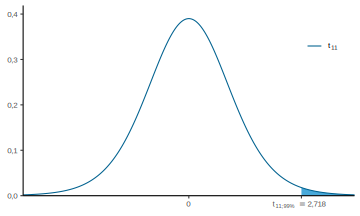
\includegraphics[width=.49\linewidth]{bookdownproj_files/figure-latex/tkrit-1} 

}

\caption{Ablehnungsbereich bei gerichteter Alternativhypothese nach oben, $n=12$ und $\alpha=0{,}01$}\label{fig:tkrit}
\end{figure}

\hypertarget{pruxfcfgruxf6uxdfe-berechnen-1}{%
\subsubsection{Prüfgröße berechnen}\label{pruxfcfgruxf6uxdfe-berechnen-1}}

Die Formel für die Berechnung der Prüfgröße \(t\) im 1-Stichproben-\(t\)-Test lautet ganz ähnlich wie die für die Prüfgröße \(z\) im \(z\)-Test -- mit dem Unterschied, dass statt der (hier unbekannten) Standardabweichung der Grundgesamtheit (\(\sigma\)) die Standardabweichung der Stichprobe (\(s\)) eingesetzt wird:

\[
t=\sqrt{n}\cdot\frac{\bar{x}-\mu_0}{s}
\]\{\#eq:t\}

Zum direkten Vergleich noch einmal die Prüfgröße im \(z\)-Test:

\[
z=\sqrt{n}\cdot\frac{\bar{x}-\mu_0}{\sigma}
\]

\hypertarget{beispiel-ausfuxfchrlich}{%
\paragraph{Beispiel (ausführlich)}\label{beispiel-ausfuxfchrlich}}

Wir erheben die Stichprobe von \(n=12\) Anträgen im Oktober und erhalten folgende Werte für die Bearbeitungsdauer (in Tagen):

\[
45\quad41\quad37\quad41\quad35\quad44\quad34\quad44\quad38\quad41\quad39\quad36
\]

Wir errechnen zunächst das arithmetische Mittel \(\bar{x}\) (s. Sitzung 2):

\[\begin{aligned}
\bar{x}&=\frac{\sum\limits_{i=1}^nx_i}{n}\\[5pt]
&=\frac{45+41+37+41+35+44+34+44+38+41+39+36}{12}\\
&\approx 39{,}58
\end{aligned}\]

Damit können wir die Standardabweichung \(s\) berechnen:

\[\begin{aligned}
s&=\sqrt{\frac{\sum\limits_{i=1}^n(x_i-\bar{x})^2}{n-1}}\\[6pt]
&\approx\sqrt{\frac{29{,}38+2{,}02+6{,}66+2{,}02+20{,}98+19{,}54+31{,}14+19{,}54+2{,}5+2{,}02+0{,}34+12{,}82}{11}}\\
&\approx 3{,}67
\end{aligned}\]

Schließlich setzen wir diese Werte in die Formel für die Prüfgröße \(t\) (\autoref{eq:t}) ein:

\[\begin{aligned}
t&=\sqrt{n}\cdot\frac{\bar{x}-\mu_0}{s}\\[6pt]
&\approx\sqrt{12}\cdot\frac{39{,}58-30{,}2}{3{,}67}\\
&\approx8{,}854
\end{aligned}\]

\hypertarget{ergebnis-interpretieren}{%
\subsubsection{Ergebnis interpretieren}\label{ergebnis-interpretieren}}

Genau wie beim \(z\)-Test kommt es darauf an, ob die Prüfgröße in den Ablehnungsbereich fällt (ob der kritische Wert also unter- bzw. überschritten wird). Wenn dies der Fall ist, können wir die Nullhypothese ablehnen (und damit unsere Alternativhypothese bestätigen). Wenn nicht, müssen wir die Nullhypothese beibehalten.

\hypertarget{beispiel-10}{%
\paragraph{Beispiel}\label{beispiel-10}}

In unserem Beispiel liegt der \(t\)-Wert deutlich über dem kritischen Wert von 2,718. Wir können also die Nullhypothese ablehnen und unsere Alternativhypothese annehmen. Unsere statistische Untersuchung hat gezeigt, dass die Bearbeitungsdauer von Anträgen, die im Oktober eingehen, länger ist als im Jahresdurchschnitt (und zwar mit Signifikanzniveau \(\alpha=0,01\)).

\begin{rtip}
In R kann ein $t$-Test mit dem Befehl {\tt t.test()} durchgeführt werden.

Neben der Prüfgröße $t$ gibt der Befehl einen $p$-Wert aus -- ist dieser kleiner als $\alpha$, so liegt eine signifikante Abweichung vor.
\end{rtip}

\hypertarget{aufgaben-4}{%
\subsection{Aufgaben}\label{aufgaben-4}}

\hypertarget{aufgabe-1-4}{%
\subsubsection{Aufgabe 1}\label{aufgabe-1-4}}

Sie interessieren sich für die durchschnittliche Haushaltsgröße in Frankfurt im europäischen Vergleich. In der EU sei die durchschnittliche Haushaltsgröße 2,30 Personen mit einer Standardabweichung von 1,42.

Sie vermuten, dass Frankfurter Haushalte sich in ihrer Größe vom europäischen Durchschnitt unterscheiden, können aber nicht sagen, in welche Richtung.

\begin{enumerate}
\def\labelenumi{\alph{enumi})}
\tightlist
\item
  Welche Stichprobengröße ist für einen \(z\)-Test in diesem Fall nötig und warum?
\item
  Formulieren Sie Null- und Alternativhypothese.
\item
  Sie entscheiden Sich für ein Signifikanzniveau von \(\alpha=0{,}05\). Notieren Sie die kritischen Werte.
\item
  Eine Stichprobe von 40 Frankfurter Haushalten ergibt eine durchschnittliche Größe von 1,82. Berechnen Sie die Prüfgröße \(z\).
\item
  Wie bewerten Sie das Ergebnis?
\end{enumerate}

\hypertarget{aufgabe-2-4}\)
\item
  \(t_{19;0,1\%}\)
\item
  \(t_{7;2,5\%}\)
\item
  \(t_{13;5\%}\)
\item
  \(t_{11;97,5\%}\)
\item
  \(t_{3;95\%}\)
\item
  \(t_{6;99,5\%}\)
\item
  \(t_{16;99,9\%}\)
\item
  \(t_{5;99\%}\)
\item
  \(t_{20;1\%}\)
\end{enumerate}

\hypertarget{aufgabe-3-2}{%
\subsubsection{Aufgabe 3}\label{aufgabe-3-2}}

Die Prüfungsergebnisse für eine Klausur im Geographiestudium seien normalverteilt mit einer mittleren Punktzahl von 61,5 und einer Standardabweichung von 10,3. Sie vermuten, dass berufstätige Studierende im Durchschnitt schlechter abschneiden, weil ihnen die Vorbereitungszeit fehlt. Eine Zufallsstichprobe berufstätiger Studierender ergibt die Prüfungsergebnisse: \texttt{42\ 78\ 46\ 65}

Prüfen Sie Ihre Vermutung. Begründen Sie die Wahl des Tests und des Signifikanzniveaus.

\hypertarget{aufgabe-4-1}{%
\subsubsection{Aufgabe 4}\label{aufgabe-4-1}}

Sie vermuten, dass Angestellte mit Migrationshintergrund in einem bestimmten Betrieb weniger als das Durchschnittsgehalt verdienen. Die Personalabteilung bestätigt Ihnen gegenüber die annähernde Normalverteilung der Bruttogehälter mit Mittelwert \(\mu=3042,43\) (in EUR). Sie planen, das Bruttogehalt von sechs zufälligen Angestellten mit Migrationshintergrund direkt zu ermitteln.\nopagebreak 

\begin{enumerate}
\def\labelenumi{\alph{enumi})}
\tightlist
\item
  Welchen Test führen Sie durch?
\item
  Formulieren Sie die Hypothesen.
\item
  Bestimmen Sie den kritischen Wert bei Signifikanzniveau \(\alpha=0{,}01\).
\end{enumerate}

\hypertarget{aufgabe-5}{%
\subsubsection{Aufgabe 5}\label{aufgabe-5}}

\emph{(Fortführung von Aufgabe 4)}

Sie ermitteln die folgenden Werte (in EUR):
\[
2927,35\quad2930,68\quad2903,58\quad3032,59\quad3013,37\quad2979,4
\]

\begin{enumerate}
\def\labelenumi{\alph{enumi})}
\tightlist
\item
  Berechnen Sie die Prüfgröße.
\item
  Welche Schlüsse ziehen Sie aus der Untersuchung?
\end{enumerate}

\hypertarget{tipps-zur-vertiefung-4}{%
\subsection{Tipps zur Vertiefung}\label{tipps-zur-vertiefung-4}}

\begin{itemize}
\tightlist
\item
  YouTube-Kanal ``Kurzes Tutorium Statistik'': \href{https://www.youtube.com/watch?v=gSyGVDMcg-U}{p-Wert, Nullhypothese, Signifikanzniveau - die Idee erklärt}
\item
  YouTube-Kanal ``Benedict K'': \href{https://www.youtube.com/watch?v=sNlxShUM4io}{p-Wert: einseitiger und beidseitiger Hypothesentest / Signifikanztest - erklärt}
\item
  YouTube-Kanal ``Kurzes Tutorium Statistik'': \href{https://www.youtube.com/watch?v=rbYg5IsOYaM}{Einstichproben t-Test}
\item
  Kapitel 7, 8.1 in \protect\hyperlink{ref-bortz}{Bortz und Schuster} (\protect\hyperlink{ref-bortz}{2010})
\item
  Kapitel 5.5.2 in \protect\hyperlink{ref-bahrenberg}{Bahrenberg, Giese und Nipper} (\protect\hyperlink{ref-bahrenberg}{2010})
\item
  Kapitel 9 in \protect\hyperlink{ref-klemm}{Klemm} (\protect\hyperlink{ref-klemm}{2002})
\end{itemize}

\pagebreak

\hypertarget{anhang-tabelle-t-verteilungen}{%
\subsection{\texorpdfstring{Anhang: Tabelle \(t\)-Verteilungen}{Anhang: Tabelle t-Verteilungen}}\label{anhang-tabelle-t-verteilungen}}

\begin{multicols}{2}
\vfill


\begin{center}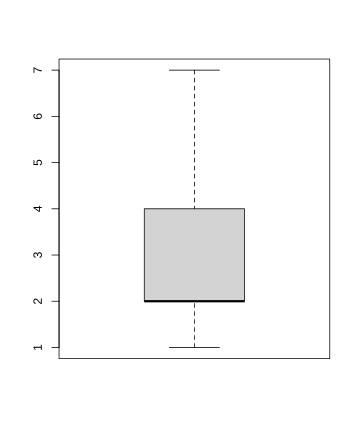
\includegraphics[width=.49\linewidth]{bookdownproj_files/figure-latex/unnamed-chunk-12-1} \end{center}
\vfill
\columnbreak
\vfill
\[ P(-t_{df})= 1 - P(t_{df}) \]
\vfill
\end{multicols}

\begin{table}[!h]
\centering
\resizebox{\linewidth}{!}{
\begin{tabular}{>{}r|rrrrrrrrrrrrrrr}
\toprule
\multicolumn{1}{c}{ } & \multicolumn{15}{c}{Fläche} \\
\cmidrule(l{3pt}r{3pt}){2-16}
$df$ & 0,55 & 0,6 & 0,65 & 0,7 & 0,75 & 0,8 & 0,85 & 0,9 & 0,95 & 0,975 & 0,99 & 0,995 & 0,999 & 0,9995 & 0,9999\\
\midrule
\cellcolor{gray!6}{1} & \cellcolor{gray!6}{0,158} & \cellcolor{gray!6}{0,325} & \cellcolor{gray!6}{0,510} & \cellcolor{gray!6}{0,727} & \cellcolor{gray!6}{1,000} & \cellcolor{gray!6}{1,376} & \cellcolor{gray!6}{1,963} & \cellcolor{gray!6}{3,078} & \cellcolor{gray!6}{6,314} & \cellcolor{gray!6}{12,706} & \cellcolor{gray!6}{31,821} & \cellcolor{gray!6}{63,657} & \cellcolor{gray!6}{318,309} & \cellcolor{gray!6}{636,619} & \cellcolor{gray!6}{3183,099}\\
2 & 0,142 & 0,289 & 0,445 & 0,617 & 0,816 & 1,061 & 1,386 & 1,886 & 2,920 & 4,303 & 6,965 & 9,925 & 22,327 & 31,599 & 70,700\\
\cellcolor{gray!6}{3} & \cellcolor{gray!6}{0,137} & \cellcolor{gray!6}{0,277} & \cellcolor{gray!6}{0,424} & \cellcolor{gray!6}{0,584} & \cellcolor{gray!6}{0,765} & \cellcolor{gray!6}{0,978} & \cellcolor{gray!6}{1,250} & \cellcolor{gray!6}{1,638} & \cellcolor{gray!6}{2,353} & \cellcolor{gray!6}{3,182} & \cellcolor{gray!6}{4,541} & \cellcolor{gray!6}{5,841} & \cellcolor{gray!6}{10,215} & \cellcolor{gray!6}{12,924} & \cellcolor{gray!6}{22,204}\\
4 & 0,134 & 0,271 & 0,414 & 0,569 & 0,741 & 0,941 & 1,190 & 1,533 & 2,132 & 2,776 & 3,747 & 4,604 & 7,173 & 8,610 & 13,034\\
\cellcolor{gray!6}{5} & \cellcolor{gray!6}{0,132} & \cellcolor{gray!6}{0,267} & \cellcolor{gray!6}{0,408} & \cellcolor{gray!6}{0,559} & \cellcolor{gray!6}{0,727} & \cellcolor{gray!6}{0,920} & \cellcolor{gray!6}{1,156} & \cellcolor{gray!6}{1,476} & \cellcolor{gray!6}{2,015} & \cellcolor{gray!6}{2,571} & \cellcolor{gray!6}{3,365} & \cellcolor{gray!6}{4,032} & \cellcolor{gray!6}{5,893} & \cellcolor{gray!6}{6,869} & \cellcolor{gray!6}{9,678}\\
\addlinespace
6 & 0,131 & 0,265 & 0,404 & 0,553 & 0,718 & 0,906 & 1,134 & 1,440 & 1,943 & 2,447 & 3,143 & 3,707 & 5,208 & 5,959 & 8,025\\
\cellcolor{gray!6}{7} & \cellcolor{gray!6}{0,130} & \cellcolor{gray!6}{0,263} & \cellcolor{gray!6}{0,402} & \cellcolor{gray!6}{0,549} & \cellcolor{gray!6}{0,711} & \cellcolor{gray!6}{0,896} & \cellcolor{gray!6}{1,119} & \cellcolor{gray!6}{1,415} & \cellcolor{gray!6}{1,895} & \cellcolor{gray!6}{2,365} & \cellcolor{gray!6}{2,998} & \cellcolor{gray!6}{3,499} & \cellcolor{gray!6}{4,785} & \cellcolor{gray!6}{5,408} & \cellcolor{gray!6}{7,063}\\
8 & 0,130 & 0,262 & 0,399 & 0,546 & 0,706 & 0,889 & 1,108 & 1,397 & 1,860 & 2,306 & 2,896 & 3,355 & 4,501 & 5,041 & 6,442\\
\cellcolor{gray!6}{9} & \cellcolor{gray!6}{0,129} & \cellcolor{gray!6}{0,261} & \cellcolor{gray!6}{0,398} & \cellcolor{gray!6}{0,543} & \cellcolor{gray!6}{0,703} & \cellcolor{gray!6}{0,883} & \cellcolor{gray!6}{1,100} & \cellcolor{gray!6}{1,383} & \cellcolor{gray!6}{1,833} & \cellcolor{gray!6}{2,262} & \cellcolor{gray!6}{2,821} & \cellcolor{gray!6}{3,250} & \cellcolor{gray!6}{4,297} & \cellcolor{gray!6}{4,781} & \cellcolor{gray!6}{6,010}\\
10 & 0,129 & 0,260 & 0,397 & 0,542 & 0,700 & 0,879 & 1,093 & 1,372 & 1,812 & 2,228 & 2,764 & 3,169 & 4,144 & 4,587 & 5,694\\
\addlinespace
\cellcolor{gray!6}{11} & \cellcolor{gray!6}{0,129} & \cellcolor{gray!6}{0,260} & \cellcolor{gray!6}{0,396} & \cellcolor{gray!6}{0,540} & \cellcolor{gray!6}{0,697} & \cellcolor{gray!6}{0,876} & \cellcolor{gray!6}{1,088} & \cellcolor{gray!6}{1,363} & \cellcolor{gray!6}{1,796} & \cellcolor{gray!6}{2,201} & \cellcolor{gray!6}{2,718} & \cellcolor{gray!6}{3,106} & \cellcolor{gray!6}{4,025} & \cellcolor{gray!6}{4,437} & \cellcolor{gray!6}{5,453}\\
12 & 0,128 & 0,259 & 0,395 & 0,539 & 0,695 & 0,873 & 1,083 & 1,356 & 1,782 & 2,179 & 2,681 & 3,055 & 3,930 & 4,318 & 5,263\\
\cellcolor{gray!6}{13} & \cellcolor{gray!6}{0,128} & \cellcolor{gray!6}{0,259} & \cellcolor{gray!6}{0,394} & \cellcolor{gray!6}{0,538} & \cellcolor{gray!6}{0,694} & \cellcolor{gray!6}{0,870} & \cellcolor{gray!6}{1,079} & \cellcolor{gray!6}{1,350} & \cellcolor{gray!6}{1,771} & \cellcolor{gray!6}{2,160} & \cellcolor{gray!6}{2,650} & \cellcolor{gray!6}{3,012} & \cellcolor{gray!6}{3,852} & \cellcolor{gray!6}{4,221} & \cellcolor{gray!6}{5,111}\\
14 & 0,128 & 0,258 & 0,393 & 0,537 & 0,692 & 0,868 & 1,076 & 1,345 & 1,761 & 2,145 & 2,624 & 2,977 & 3,787 & 4,140 & 4,985\\
\cellcolor{gray!6}{15} & \cellcolor{gray!6}{0,128} & \cellcolor{gray!6}{0,258} & \cellcolor{gray!6}{0,393} & \cellcolor{gray!6}{0,536} & \cellcolor{gray!6}{0,691} & \cellcolor{gray!6}{0,866} & \cellcolor{gray!6}{1,074} & \cellcolor{gray!6}{1,341} & \cellcolor{gray!6}{1,753} & \cellcolor{gray!6}{2,131} & \cellcolor{gray!6}{2,602} & \cellcolor{gray!6}{2,947} & \cellcolor{gray!6}{3,733} & \cellcolor{gray!6}{4,073} & \cellcolor{gray!6}{4,880}\\
\addlinespace
16 & 0,128 & 0,258 & 0,392 & 0,535 & 0,690 & 0,865 & 1,071 & 1,337 & 1,746 & 2,120 & 2,583 & 2,921 & 3,686 & 4,015 & 4,791\\
\cellcolor{gray!6}{17} & \cellcolor{gray!6}{0,128} & \cellcolor{gray!6}{0,257} & \cellcolor{gray!6}{0,392} & \cellcolor{gray!6}{0,534} & \cellcolor{gray!6}{0,689} & \cellcolor{gray!6}{0,863} & \cellcolor{gray!6}{1,069} & \cellcolor{gray!6}{1,333} & \cellcolor{gray!6}{1,740} & \cellcolor{gray!6}{2,110} & \cellcolor{gray!6}{2,567} & \cellcolor{gray!6}{2,898} & \cellcolor{gray!6}{3,646} & \cellcolor{gray!6}{3,965} & \cellcolor{gray!6}{4,714}\\
18 & 0,127 & 0,257 & 0,392 & 0,534 & 0,688 & 0,862 & 1,067 & 1,330 & 1,734 & 2,101 & 2,552 & 2,878 & 3,610 & 3,922 & 4,648\\
\cellcolor{gray!6}{19} & \cellcolor{gray!6}{0,127} & \cellcolor{gray!6}{0,257} & \cellcolor{gray!6}{0,391} & \cellcolor{gray!6}{0,533} & \cellcolor{gray!6}{0,688} & \cellcolor{gray!6}{0,861} & \cellcolor{gray!6}{1,066} & \cellcolor{gray!6}{1,328} & \cellcolor{gray!6}{1,729} & \cellcolor{gray!6}{2,093} & \cellcolor{gray!6}{2,539} & \cellcolor{gray!6}{2,861} & \cellcolor{gray!6}{3,579} & \cellcolor{gray!6}{3,883} & \cellcolor{gray!6}{4,590}\\
20 & 0,127 & 0,257 & 0,391 & 0,533 & 0,687 & 0,860 & 1,064 & 1,325 & 1,725 & 2,086 & 2,528 & 2,845 & 3,552 & 3,850 & 4,539\\
\addlinespace
\cellcolor{gray!6}{25} & \cellcolor{gray!6}{0,127} & \cellcolor{gray!6}{0,256} & \cellcolor{gray!6}{0,390} & \cellcolor{gray!6}{0,531} & \cellcolor{gray!6}{0,684} & \cellcolor{gray!6}{0,856} & \cellcolor{gray!6}{1,058} & \cellcolor{gray!6}{1,316} & \cellcolor{gray!6}{1,708} & \cellcolor{gray!6}{2,060} & \cellcolor{gray!6}{2,485} & \cellcolor{gray!6}{2,787} & \cellcolor{gray!6}{3,450} & \cellcolor{gray!6}{3,725} & \cellcolor{gray!6}{4,352}\\
30 & 0,127 & 0,256 & 0,389 & 0,530 & 0,683 & 0,854 & 1,055 & 1,310 & 1,697 & 2,042 & 2,457 & 2,750 & 3,385 & 3,646 & 4,234\\
\cellcolor{gray!6}{35} & \cellcolor{gray!6}{0,127} & \cellcolor{gray!6}{0,255} & \cellcolor{gray!6}{0,388} & \cellcolor{gray!6}{0,529} & \cellcolor{gray!6}{0,682} & \cellcolor{gray!6}{0,852} & \cellcolor{gray!6}{1,052} & \cellcolor{gray!6}{1,306} & \cellcolor{gray!6}{1,690} & \cellcolor{gray!6}{2,030} & \cellcolor{gray!6}{2,438} & \cellcolor{gray!6}{2,724} & \cellcolor{gray!6}{3,340} & \cellcolor{gray!6}{3,591} & \cellcolor{gray!6}{4,153}\\
40 & 0,126 & 0,255 & 0,388 & 0,529 & 0,681 & 0,851 & 1,050 & 1,303 & 1,684 & 2,021 & 2,423 & 2,704 & 3,307 & 3,551 & 4,094\\
\cellcolor{gray!6}{45} & \cellcolor{gray!6}{0,126} & \cellcolor{gray!6}{0,255} & \cellcolor{gray!6}{0,388} & \cellcolor{gray!6}{0,528} & \cellcolor{gray!6}{0,680} & \cellcolor{gray!6}{0,850} & \cellcolor{gray!6}{1,049} & \cellcolor{gray!6}{1,301} & \cellcolor{gray!6}{1,679} & \cellcolor{gray!6}{2,014} & \cellcolor{gray!6}{2,412} & \cellcolor{gray!6}{2,690} & \cellcolor{gray!6}{3,281} & \cellcolor{gray!6}{3,520} & \cellcolor{gray!6}{4,049}\\
\addlinespace
50 & 0,126 & 0,255 & 0,388 & 0,528 & 0,679 & 0,849 & 1,047 & 1,299 & 1,676 & 2,009 & 2,403 & 2,678 & 3,261 & 3,496 & 4,014\\
\cellcolor{gray!6}{55} & \cellcolor{gray!6}{0,126} & \cellcolor{gray!6}{0,255} & \cellcolor{gray!6}{0,387} & \cellcolor{gray!6}{0,527} & \cellcolor{gray!6}{0,679} & \cellcolor{gray!6}{0,848} & \cellcolor{gray!6}{1,046} & \cellcolor{gray!6}{1,297} & \cellcolor{gray!6}{1,673} & \cellcolor{gray!6}{2,004} & \cellcolor{gray!6}{2,396} & \cellcolor{gray!6}{2,668} & \cellcolor{gray!6}{3,245} & \cellcolor{gray!6}{3,476} & \cellcolor{gray!6}{3,986}\\
60 & 0,126 & 0,254 & 0,387 & 0,527 & 0,679 & 0,848 & 1,045 & 1,296 & 1,671 & 2,000 & 2,390 & 2,660 & 3,232 & 3,460 & 3,962\\
\cellcolor{gray!6}{65} & \cellcolor{gray!6}{0,126} & \cellcolor{gray!6}{0,254} & \cellcolor{gray!6}{0,387} & \cellcolor{gray!6}{0,527} & \cellcolor{gray!6}{0,678} & \cellcolor{gray!6}{0,847} & \cellcolor{gray!6}{1,045} & \cellcolor{gray!6}{1,295} & \cellcolor{gray!6}{1,669} & \cellcolor{gray!6}{1,997} & \cellcolor{gray!6}{2,385} & \cellcolor{gray!6}{2,654} & \cellcolor{gray!6}{3,220} & \cellcolor{gray!6}{3,447} & \cellcolor{gray!6}{3,942}\\
70 & 0,126 & 0,254 & 0,387 & 0,527 & 0,678 & 0,847 & 1,044 & 1,294 & 1,667 & 1,994 & 2,381 & 2,648 & 3,211 & 3,435 & 3,926\\
\addlinespace
\cellcolor{gray!6}{75} & \cellcolor{gray!6}{0,126} & \cellcolor{gray!6}{0,254} & \cellcolor{gray!6}{0,387} & \cellcolor{gray!6}{0,527} & \cellcolor{gray!6}{0,678} & \cellcolor{gray!6}{0,846} & \cellcolor{gray!6}{1,044} & \cellcolor{gray!6}{1,293} & \cellcolor{gray!6}{1,665} & \cellcolor{gray!6}{1,992} & \cellcolor{gray!6}{2,377} & \cellcolor{gray!6}{2,643} & \cellcolor{gray!6}{3,202} & \cellcolor{gray!6}{3,425} & \cellcolor{gray!6}{3,911}\\
80 & 0,126 & 0,254 & 0,387 & 0,526 & 0,678 & 0,846 & 1,043 & 1,292 & 1,664 & 1,990 & 2,374 & 2,639 & 3,195 & 3,416 & 3,899\\
\cellcolor{gray!6}{90} & \cellcolor{gray!6}{0,126} & \cellcolor{gray!6}{0,254} & \cellcolor{gray!6}{0,387} & \cellcolor{gray!6}{0,526} & \cellcolor{gray!6}{0,677} & \cellcolor{gray!6}{0,846} & \cellcolor{gray!6}{1,042} & \cellcolor{gray!6}{1,291} & \cellcolor{gray!6}{1,662} & \cellcolor{gray!6}{1,987} & \cellcolor{gray!6}{2,368} & \cellcolor{gray!6}{2,632} & \cellcolor{gray!6}{3,183} & \cellcolor{gray!6}{3,402} & \cellcolor{gray!6}{3,878}\\
100 & 0,126 & 0,254 & 0,386 & 0,526 & 0,677 & 0,845 & 1,042 & 1,290 & 1,660 & 1,984 & 2,364 & 2,626 & 3,174 & 3,390 & 3,862\\
\cellcolor{gray!6}{110} & \cellcolor{gray!6}{0,126} & \cellcolor{gray!6}{0,254} & \cellcolor{gray!6}{0,386} & \cellcolor{gray!6}{0,526} & \cellcolor{gray!6}{0,677} & \cellcolor{gray!6}{0,845} & \cellcolor{gray!6}{1,041} & \cellcolor{gray!6}{1,289} & \cellcolor{gray!6}{1,659} & \cellcolor{gray!6}{1,982} & \cellcolor{gray!6}{2,361} & \cellcolor{gray!6}{2,621} & \cellcolor{gray!6}{3,166} & \cellcolor{gray!6}{3,381} & \cellcolor{gray!6}{3,848}\\
\addlinespace
120 & 0,126 & 0,254 & 0,386 & 0,526 & 0,677 & 0,845 & 1,041 & 1,289 & 1,658 & 1,980 & 2,358 & 2,617 & 3,160 & 3,373 & 3,837\\
\cellcolor{gray!6}{130} & \cellcolor{gray!6}{0,126} & \cellcolor{gray!6}{0,254} & \cellcolor{gray!6}{0,386} & \cellcolor{gray!6}{0,526} & \cellcolor{gray!6}{0,676} & \cellcolor{gray!6}{0,844} & \cellcolor{gray!6}{1,041} & \cellcolor{gray!6}{1,288} & \cellcolor{gray!6}{1,657} & \cellcolor{gray!6}{1,978} & \cellcolor{gray!6}{2,355} & \cellcolor{gray!6}{2,614} & \cellcolor{gray!6}{3,154} & \cellcolor{gray!6}{3,367} & \cellcolor{gray!6}{3,828}\\
140 & 0,126 & 0,254 & 0,386 & 0,526 & 0,676 & 0,844 & 1,040 & 1,288 & 1,656 & 1,977 & 2,353 & 2,611 & 3,149 & 3,361 & 3,820\\
\cellcolor{gray!6}{150} & \cellcolor{gray!6}{0,126} & \cellcolor{gray!6}{0,254} & \cellcolor{gray!6}{0,386} & \cellcolor{gray!6}{0,526} & \cellcolor{gray!6}{0,676} & \cellcolor{gray!6}{0,844} & \cellcolor{gray!6}{1,040} & \cellcolor{gray!6}{1,287} & \cellcolor{gray!6}{1,655} & \cellcolor{gray!6}{1,976} & \cellcolor{gray!6}{2,351} & \cellcolor{gray!6}{2,609} & \cellcolor{gray!6}{3,145} & \cellcolor{gray!6}{3,357} & \cellcolor{gray!6}{3,813}\\
200 & 0,126 & 0,254 & 0,386 & 0,525 & 0,676 & 0,843 & 1,039 & 1,286 & 1,653 & 1,972 & 2,345 & 2,601 & 3,131 & 3,340 & 3,789\\
\addlinespace
\cellcolor{gray!6}{300} & \cellcolor{gray!6}{0,126} & \cellcolor{gray!6}{0,254} & \cellcolor{gray!6}{0,386} & \cellcolor{gray!6}{0,525} & \cellcolor{gray!6}{0,675} & \cellcolor{gray!6}{0,843} & \cellcolor{gray!6}{1,038} & \cellcolor{gray!6}{1,284} & \cellcolor{gray!6}{1,650} & \cellcolor{gray!6}{1,968} & \cellcolor{gray!6}{2,339} & \cellcolor{gray!6}{2,592} & \cellcolor{gray!6}{3,118} & \cellcolor{gray!6}{3,323} & \cellcolor{gray!6}{3,765}\\
400 & 0,126 & 0,254 & 0,386 & 0,525 & 0,675 & 0,843 & 1,038 & 1,284 & 1,649 & 1,966 & 2,336 & 2,588 & 3,111 & 3,315 & 3,754\\
\cellcolor{gray!6}{500} & \cellcolor{gray!6}{0,126} & \cellcolor{gray!6}{0,253} & \cellcolor{gray!6}{0,386} & \cellcolor{gray!6}{0,525} & \cellcolor{gray!6}{0,675} & \cellcolor{gray!6}{0,842} & \cellcolor{gray!6}{1,038} & \cellcolor{gray!6}{1,283} & \cellcolor{gray!6}{1,648} & \cellcolor{gray!6}{1,965} & \cellcolor{gray!6}{2,334} & \cellcolor{gray!6}{2,586} & \cellcolor{gray!6}{3,107} & \cellcolor{gray!6}{3,310} & \cellcolor{gray!6}{3,747}\\
1000 & 0,126 & 0,253 & 0,385 & 0,525 & 0,675 & 0,842 & 1,037 & 1,282 & 1,646 & 1,962 & 2,330 & 2,581 & 3,098 & 3,300 & 3,733\\
\cellcolor{gray!6}{$z$} & \cellcolor{gray!6}{0,126} & \cellcolor{gray!6}{0,253} & \cellcolor{gray!6}{0,385} & \cellcolor{gray!6}{0,524} & \cellcolor{gray!6}{0,674} & \cellcolor{gray!6}{0,842} & \cellcolor{gray!6}{1,036} & \cellcolor{gray!6}{1,282} & \cellcolor{gray!6}{1,645} & \cellcolor{gray!6}{1,960} & \cellcolor{gray!6}{2,326} & \cellcolor{gray!6}{2,576} & \cellcolor{gray!6}{3,090} & \cellcolor{gray!6}{3,291} & \cellcolor{gray!6}{3,719}\\
\bottomrule
\end{tabular}}
\end{table}

\pagebreak

\hypertarget{quellen-4}{%
\subsection{Quellen}\label{quellen-4}}

\hypertarget{testverfahren-mit-zwei-stichproben}{%
\section{Testverfahren mit zwei Stichproben}\label{testverfahren-mit-zwei-stichproben}}

\hypertarget{lernziele-dieser-sitzung-5}{%
\subsection{Lernziele dieser Sitzung}\label{lernziele-dieser-sitzung-5}}

Sie können\ldots{}

\begin{itemize}
\tightlist
\item
  einen 2-Stichproben-\(t\)-Test durchführen.
\item
  einen \(F\)-Test durchführen.
\item
  Fehler 1. und 2. Art unterscheiden.
\end{itemize}

\hypertarget{statistische-tests-1}{%
\subsection{Statistische Tests}\label{statistische-tests-1}}

In Sitzung 5 haben wir mit dem \(z\)-Test und dem 1-Stichproben-\(t\)-Test die ersten Testverfahren kennengelernt. In dieser Sitzung kommt der 2-Stichproben-\(t\)-Test sowie der \(F\)-Test dazu.

Das grundsätzliche Verfahren bleibt dabei stets das gleiche. Zur Erinnerung noch einmal die sechs Schritte:

\begin{enumerate}
\def\labelenumi{\arabic{enumi}.}
\tightlist
\item
  Test auswählen und Voraussetzungen prüfen
\item
  Hypothesen formulieren
\item
  Signifikanzniveau entscheiden
\item
  Ablenhnungsbereich bestimmen
\item
  Prüfgröße berechnen
\item
  Ergebnis interpretieren
\end{enumerate}

\hypertarget{stichproben-t-test-1}{%
\subsection{\texorpdfstring{2-Stichproben-\(t\)-Test}{2-Stichproben-t-Test}}\label{stichproben-t-test-1}}

Bei der folgenden Variante des \(t\)-Tests (und beim \(F\)-Test) wird nicht wie gehabt \emph{eine} Stichprobe auf signifikante Abweichungen \emph{von der Grundgesamtheit} überprüft, sondern \emph{zwei} Stichproben auf signifikante Abweichungen \emph{voneinander.} An den sechs Schritten ändert sich nichts.

Den 2-Stichproben-\(t\)-Test gibt es je nach Voraussetzungen bzw. Annahmen in vielen unterschiedlichen Varianten. In dieser Veranstaltung wird nur eine bestimmte (vergleichsweise einfache) Variante behandelt. In der Praxis geht es aber oft darum, für ganz bestimmte empirische Bedinungen den „richtigen`` 2-Stichproben-\(t\)-Test auszuwählen.

Die hier behandelte Variante soll mit folgendem Beispiel illustriert werden: Wir interessieren uns für die Mietpreise von kleine Gewerbeflächen in den beiden Frankfurter Stadtteilen Höchst und Praunheim. Wir vermuten, dass es einen signifikanten Unterschied gibt, wissen aber nicht in welche Richtung. Wir planen eine Befragung von je 6 Mieter*innen von kleinen Gewerberäumen, die nach Zufallsprinzip ausgewählt werden.

\hypertarget{test-wuxe4hlen-und-voraussetzungen-pruxfcfen-2}{%
\subsubsection{Test wählen und Voraussetzungen prüfen}\label{test-wuxe4hlen-und-voraussetzungen-pruxfcfen-2}}

Der hier behandelte 2-Stichproben-\(t\)-Test hat folgende Voraussetzungen (bzw. Annahmen):

\begin{itemize}
\tightlist
\item
  Es soll untersucht werden, ob ein Merkmal in zwei Stichproben signifikant voneinander abweicht.
\item
  Die Stichproben sind einfache Zufallsstichproben und unabhängig voneinander erhoben.
\item
  Die Stichproben haben dieselbe Anzahl an Elementen (\(n_1=n_2\)).
\item
  Das Merkmal ist grundsätzlich (annähernd) normalverteilt.
\item
  Die Varianzen der zu vergleichenden Populationen sind gleich (\(\sigma^2_1=\sigma^2_2\)).\footnote{Diese Voraussetzung ist etwas merkwürdig, denn beim \(t\)-Test kennen wir ja die Varianzen der Grundgesamtheiten gar nicht. \protect\hyperlink{f}{Der \(F\)-Test} kann diese Voraussetzung anhand der Stichprobenverteilungen prüfen.}
\end{itemize}

\hypertarget{beispiel-11}{%
\paragraph{Beispiel}\label{beispiel-11}}

Probleme bereiten hier die Voraussetzungen der Normalverteilung und der gleichen Varianzen. Mit der Annahme der Normalverteilung können wir leben (weil wir uns mit Statistik gut auskennen und wissen, dass der \(t\)-Test „robust`` auf nicht-ganz-normalverteilte Merkmale reagiert). Wenn sich während des Tests jedoch herausstellen sollte, dass die Varianzen zu unterschiedlich sind, müssten wir das Vorgehen neu überdenken.

\hypertarget{hypothesen-formulieren-2}{%
\subsubsection{Hypothesen formulieren}\label{hypothesen-formulieren-2}}

Im Unterschied zu zuvor besprochenen Verfahren gibt es hier keine übergeordnete Grundgesamtheit, und damit kein \(\mu_0\). Stattdessen werden Hypothesen über die Populationen der beiden Stichproben (\(\mu_1\) und \(\mu_2\)) formuliert.

\hypertarget{nullhypothese-2}{%
\paragraph{Nullhypothese}\label{nullhypothese-2}}

Die Nullhypothese geht davon aus, dass es keinen Unterschied zwischen den beiden Populationen gibt. Sie lautet daher:

\[
H_0 : \mu_1 = \mu_2
\]\{\#eq: h20\}

\hypertarget{alternativhypothese-2}{%
\paragraph{Alternativhypothese}\label{alternativhypothese-2}}

Die Alternativhypothese stellt üblicherweise die forscherische Vermutung dar, die überprüft werden soll. Dabei gibt es auch hier zwei unterschiedliche Möglichkeiten: ungerichtete und gerichtete Alternativhypothesen.

\hypertarget{ungerichtete-alternativhypothese-1}{%
\subparagraph{Ungerichtete Alternativhypothese}\label{ungerichtete-alternativhypothese-1}}

Die ungerichtete Alternativhypothese besagt nur, \emph{dass} es einen Unterschied zwischen \(\mu_1\) und \(\mu_2\) gibt, aber nicht in welche Richtung (größer oder kleiner). Sie lautet daher:

\[
H_1 : \mu_1 \neq \mu_2
\]\{\#eq:h21u\}

\hypertarget{gerichtete-alternativhypothese-1}{%
\subparagraph{Gerichtete Alternativhypothese}\label{gerichtete-alternativhypothese-1}}

Die gerichtete Alternativhyptothese gibt eine Richtung des vermuteten Unterschieds vor. Sie lautet entweder:

\[
H_1 : \mu_1 < \mu_2
\]\{\#eq:h21l\}

oder:

\[
H_1 : \mu_1 > \mu_2
\]\{\#eq:h21g\}

\hypertarget{beispiel-12}{%
\paragraph{Beispiel}\label{beispiel-12}}

Wir vermuten zwar einen Unterschied, wissen aber nicht in welche Richtung. Deshalb formulieren wir neben der Nullhypothese eine ungerichtete Alternativhypothese:

\[\begin{aligned}
H_0 : \mu_1 = \mu_2\\[4pt]
H_1 : \mu_1 \neq \mu_2
\end{aligned}\]

\hypertarget{signifikanzniveau-entscheiden-2}{%
\subsubsection{Signifikanzniveau entscheiden}\label{signifikanzniveau-entscheiden-2}}

Wie auch sonst sind übliche Werte hier \(\alpha=0{,}01\) und \(\alpha=0{,}05\).

\hypertarget{beispiel-13}{%
\paragraph{Beispiel}\label{beispiel-13}}

Wir entscheiden uns für das Signifikanzniveau \(\alpha=0{,}05\).

\hypertarget{ablehnungsbereich-bestimmen-2}{%
\subsubsection{Ablehnungsbereich bestimmen}\label{ablehnungsbereich-bestimmen-2}}

Der kritische Wert wird genau wie bei dem 1-Stichproben-\(t\)-Test aus der Tabelle abgelesen. Der einzige (wichtige!) Unterschied ist die Bestimmung der Freiheitsgrade: Bei zwei Stichproben der Größe \(n\) werden die Freiheitsgrade bestimmt durch:

\[
\mathit{df}=2\cdot n -2
\]\{\#eq:df2sp\}

\hypertarget{beispiel-14} \quad \textrm{und} \quad t \geq t_{10;97{,}5\%}\\[4pt]
t &\leq -2{,}228 \quad \textrm{und} \quad t \geq 2{,}228
\end{aligned}\]

\hypertarget{pruxfcfgruxf6uxdfe-berechnen-2}{%
\subsubsection{Prüfgröße berechnen}\label{pruxfcfgruxf6uxdfe-berechnen-2}}

Bei zwei Stichproben mit Mittelwert \(\bar{x}_1\) bzw. \(\bar{x}_1\) und Varianz \(s^2_1\) bzw. \(s^2_2\) lautet die Formel zur Bestimmung der Prüfgröße \(t\):

\[
t=\frac{\bar{x}_1-\bar{x}_2}{\sqrt{\frac{s^2_1+s^2_2}{n}}}
\]\{\#eq:t2sp\}

\hypertarget{beispiel-15}{%
\paragraph{Beispiel}\label{beispiel-15}}

Wir erheben folgende Werte für die Kaltmiete pro m²:

\[\begin{aligned}
\textrm{Höchst} (x_1):\quad7{,}96\quad8{,}46\quad7{,}13\quad8{,}95\quad7{,}62\quad8{,}22\\[4pt]
\textrm{Praunheim} (x_2):\quad5{,}54\quad5{,}80\quad8{,}70\quad7{,}99\quad6{,}23\quad6{,}75
\end{aligned}\]

Für die arithmetischen Mittel ergibt sich (s. Sitzung 2):

\[\begin{aligned}
\bar{x}_1\approx8{,}06\\[4pt]
\bar{x}_2\approx6{,}84
\end{aligned}\]

Die Varianzen (s. Sitzung 2):

\[\begin{aligned}
s^2_1\approx0{,}41\\[4pt]
s^2_2\approx1{,}59
\end{aligned}\]

Diese Varianzen sehen auf den ersten Blick sehr unterschiedlich aus, was ein Problem ist: Der 2-Stichproben-\(t\)-Test hat ja zur Annahme, dass die Varianzen in den beiden Populationen gleich sind.

Andererseits sind ja auch die Stichprobenvarianzen zu einem gewissen Grad Zufallsprodukte, und diese beiden Varianzen bewegen sich auch irgendwie noch in der selben Größenordnung -- schließlich könnten sie auch 0,1 und 20 lauten.

Wir entscheiden uns zunächst dazu, den Test fortzuführen und lernen gleich eine Methode kennen, wie wir überprüfen können, ob das auch gerechtfertigt ist.

Um die Prüfgröße \(t\) zu bestimmen, setzen wir einfach unsere Stichprobenwerte in die Formel aus \autoref{eq:t2sp} ein:

\[\begin{aligned}
t&=\frac{\bar{x}_1-\bar{x}_2}{\sqrt{\frac{s^2_1+s^2_2}{n}}}\\[6pt]
&\approx\frac{8{,}06-6{,}84}{\sqrt{\frac{0{,}41+1{,}59}{6}}}\\[4pt]
&\approx2{,}113
\end{aligned}\]

\hypertarget{ergebnis-interpretieren-1}{%
\subsubsection{Ergebnis interpretieren}\label{ergebnis-interpretieren-1}}

Genau wie bei den anderen Tests wird je nach erreichen des kritischen Werts (des Ablehnungsbereichs) die Nullhypothese verworfen oder beibehalten.

\hypertarget{beispiel-16}{%
\paragraph{Beispiel}\label{beispiel-16}}

Der kritische Wert von \(t \geq 2{,}228\) wurde nicht überschritten. Wir müssen die Nullhypothese beibehalten, d.h. wir konnten keinen signifikanten Unterschied zwischen den Mietpreisen in Höchst und Praunheim feststellen (\(\alpha=0{,}05\)).

\begin{rtip}
In R wird auch der 2-Stichproben-$t$-Test mit dem Befehl {\tt t.test()} durchgeführt. Im Gegensatz zum 1-Stichproben-$t$-Test werden dabei zwei Verteilungen als Argumente eingegeben.
\end{rtip}

\hypertarget{die-f-verteilung}{%
\subsection{\texorpdfstring{Die \(F\)-Verteilung}{Die F-Verteilung}}\label{die-f-verteilung}}

Die Prüfgröße \(F\) im \(F\)-Test ist unter Annahme der Nullhypothese \(F\)-verteilt. Im Gegensatz zu den Verteilungen von \(z\) und \(t\) ist die \(F\)-Verteilung nicht symmetrisch und nimmt nur positive Werte an (s. \autoref{fig:fdf}).

Dazu ist die \(F\)-Verteilung nicht wie \(t\) von einem, sondern von zwei Freiheitsgraden abhängig. Die Reihenfolge dieser Freiheitsgrade ist auch wichtig: Wir sprechen vom Zähler-Freiheitsgrad (\(\mathit{df}_1\)) und vom Nenner-Freiheitsgrad (\(\mathit{df}_2\)). Die \(F\)-Verteilung wird also notiert mit: \(F_{\mathit{df}_1;\mathit{df}_2}\)

\begin{figure}[h]

{\centering 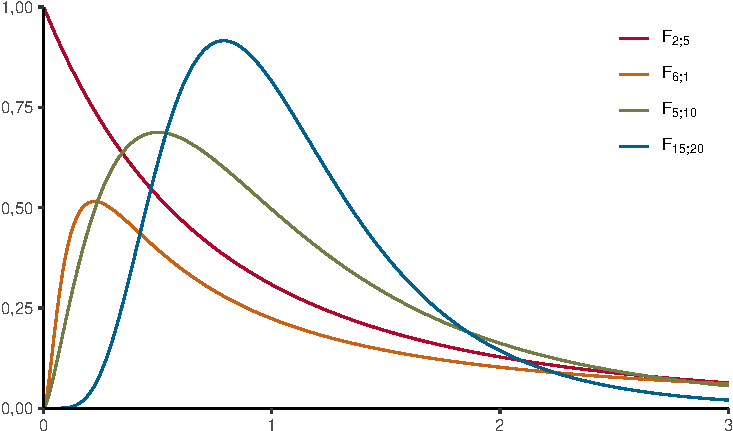
\includegraphics[width=.49\linewidth]{bookdownproj_files/figure-latex/fdf-1} 

}

\caption{$F$-Verteilungen mit verschiedenen Freiheitsgraden}\label{fig:fdf}
\end{figure}

\hypertarget{f}{%
\subsection{\texorpdfstring{\(F\)-Test}{F-Test}}\label{f}}

Auch der \(F\)-Test untersucht zwei unabhängige Stichproben. Er unterscheidet sich jedoch insofern grundlegend von den zuvor besprochenen Testverfahren, als dass sein Untersuchungsgegenstand nicht der Mittelwert (\(\mu\)) sondern die Varianz (\(\sigma^2\)) der beiden Populationen ist.

Die Prüfgröße \(F\) ist dann unter Annahme der Nullhypothese \(F\)-verteilt.

Unser Beispiel ist eine Fortführung des vorigen Beispiels für den 2-Stichproben-\(t\)-Test (Mietpreise für Gewerbeflächen). Uns interessiert: Sind die Varianzen eventuell so unterschiedlich, dass wir den obigen \(t\)-Test gar nicht hätten durchführen dürfen?

\hypertarget{test-wuxe4hlen-und-voraussetzungen-pruxfcfen-3}{%
\subsubsection{Test wählen und Voraussetzungen prüfen}\label{test-wuxe4hlen-und-voraussetzungen-pruxfcfen-3}}

Das Ziel des \(F\)-Tests ist die Feststellung eines signifikanten Unterschieds in der Varianz von zwei Populationen. Die Voraussetzungen lauten:

\begin{itemize}
\tightlist
\item
  Ausgangspunkt sind zwei unabhängig voneinander erhobene Stichproben (die aber grundsätzlich unterschiedlich groß sein dürfen).
\item
  Das Merkmal ist in beiden Populationen (annähernd) normalverteilt.
\end{itemize}

\hypertarget{beispiel-17}{%
\paragraph{Beispiel}\label{beispiel-17}}

Die Voraussetzung der Normalverteilung ist hier besonders wichtig, denn der Test wird bei anderen Verteilungen stark verfälscht. (Der \(F\)-Test ist also nicht „robust``, was die Normalverteilung angeht.)

Wir müssen also explizit die Annahme treffen, dass die Mietpreise annähernd normalverteilt sind. Das ist einerseits nicht ganz abwegig, andererseits würden wir in der Praxis unsere statistische Untersuchung dadurch angreifbar machen.

\hypertarget{hypothesen-formulieren-3}{%
\subsubsection{Hypothesen formulieren}\label{hypothesen-formulieren-3}}

Alles wie gehabt -- nur, dass es um die Varianz \(\sigma^2\) der jewiligen Populationen geht.

\hypertarget{nullhypothese-3}{%
\paragraph{Nullhypothese}\label{nullhypothese-3}}

\[
H_0: \sigma^2_1=\sigma^2_2
\]\{\#eq:h0f\}

\hypertarget{alternativhypothesen}{%
\paragraph{Alternativhypothesen}\label{alternativhypothesen}}

\hypertarget{ungerichtet}{%
\subparagraph{Ungerichtet}\label{ungerichtet}}

\[
H_1: \sigma^2_1\neq\sigma^2_2
\]\{\#eq:h1uf\}

\hypertarget{gerichtet}{%
\subparagraph{Gerichtet}\label{gerichtet}}

\[
H_1: \sigma^2_1>\sigma^2_2
\]\{\#eq:h1gf\}
oder
\[
H_1: \sigma^2_1<\sigma^2_2
\]\{\#eq:h1lf\}

\hypertarget{beispiel-18}{%
\paragraph{Beispiel}\label{beispiel-18}}

Die Nullhypothese ist einfach:

\[
H_0: \sigma^2_1=\sigma^2_2
\]

Bei der Alternativhypothese ist die Ausgangslage, dass wir empirisch einen Unterschied zwischen \(s^2_1\approx0{,}41\) und \(s^2_2\approx1{,}59\) festgestellt haben. Die Frage, ob die Varianz der Mietpreise in Höchst \emph{tatsächlich signifikant kleiner} ist, wird übersetzt in die Alternativhypothese:

\[
H_1: \sigma^2_1<\sigma^2_2
\]

Interessanterweise wäre hier (zur Abwechslung) das forscherische Interesse, die Nullhypothese beizubehalten -- denn wir wollen ja den \(t\)-Test durchführen dürfen.

\hypertarget{signifikanzniveau-entscheiden-3}{%
\subsubsection{Signifikanzniveau entscheiden}\label{signifikanzniveau-entscheiden-3}}

Die Logik ist hier genau dieselbe: Wie unwahrscheinlich muss das empirische Ergebnis unter Annahme der Nullhypothese sein, damit wir diese ablehnen (müssen)?

\hypertarget{beispiel-19}{%
\paragraph{Beispiel}\label{beispiel-19}}

Wir entscheiden uns für das (für unsere Zwecke sehr übliche) Signifikanzniveau von \(\alpha=0{,}05\).

\hypertarget{ablehnungsbereich-bestimmen-3}{%
\subsubsection{Ablehnungsbereich bestimmen}\label{ablehnungsbereich-bestimmen-3}}

Für die ungerichtete Alternativhypothese sind die kritischen Werte:

\[
F \leq F_{\mathit{df}_1;\mathit{df}_2;\alpha/2} \quad \textrm{und} \quad F \geq F_{\mathit{df}_1;\mathit{df}_2;(1-\alpha/2)}
\]\{\#eq:kritFu\}

Für die gerichtete Alternativhypothese:
\[
F \leq F_{\mathit{df}_1;\mathit{df}_2;\alpha}
\]\{\#eq:kritFl\}

bzw.

\[
F \geq F_{\mathit{df}_1;\mathit{df}_2;(1-\alpha)}
\]\{\#eq:kritFg\}

Die Besonderheit der \(F\)-Verteilung ist, dass sie gleich von zwei Freiheitsgraden abhängt: dem Zähler-Freiheitsgrad \(\mathit{df}_1\) und dem Nenner-Freiheitsgrad \(\mathit{df}_2\).

Dabei bestimmen sich die Freiheitsgrade wieder durch die Stichprobengrößen:

\[\begin{aligned}
\mathit{df}_1=n_1-1\\
\mathit{df}_2=n_2-1
\end{aligned}\]\{\#eq:Fdfs\}

In der Tabelle im Anhang sind nur die Werte für Flächenanteile von 0,95 vermerkt. Die Werte für Flächenanteile von 0,05 (also am linken Rand) können durch \autoref{eq:Frev} bestimmt werden:

\[
F_{\mathit{df}_1;\mathit{df}_2;\alpha}=\frac{1}{F_{\mathit{df}_2;\mathit{df}_1;(1-\alpha)}} 
\]\{\#eq:Frev\}

Dabei ist zu beachten, dass im Nenner die Reihenfolge der Freiheitsgrade getauscht wird!

Zur Verdeutlichung könnte -- losgelöst von unserem Beispiel -- ein unterer kritischer Wert berechnet werden durch:

\[\begin{aligned}
F_{13;20;5\%}&=\frac{1}{F_{20;13;95\%}} \\[5pt]
&\approx\frac{1}{2{,}46}\approx0{,}41
\end{aligned}\]

\hypertarget{beispiel-20}\\[5pt]
F &\leq \frac{1}{F_{5;5;95\%}}\\[5pt]
F &\leq \frac{1}{5{,}05}\\[4pt]
F &\leq 0{,}20\\[4pt]
\end{aligned}\]

Der so berechnete Ablehnungsbereich ist grafisch in \autoref{fig:falpha} aufbereitet.

\begin{figure}[h]

{\centering 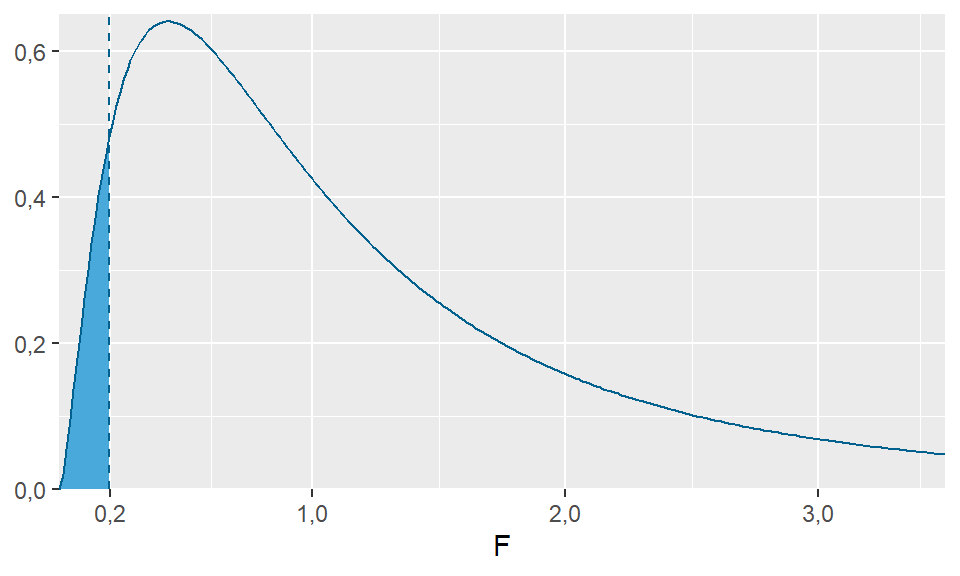
\includegraphics[width=.49\linewidth]{bookdownproj_files/figure-latex/falpha-1} 

}

\caption{Ablehnungsbereich für $F \leq F_{5;5;5\%}$}\label{fig:falpha}
\end{figure}

\hypertarget{pruxfcfgruxf6uxdfe-berechnen-3}{%
\subsubsection{Prüfgröße berechnen}\label{pruxfcfgruxf6uxdfe-berechnen-3}}

Die Formel für die Prüfgröße \(F\) ist denkbar einfach:

\[\begin{aligned}
F=\frac{s^2_1}{s^2_2}
\end{aligned}\]\{\#eq:formelf\}

\hypertarget{beispiel-21}{%
\paragraph{Beispiel}\label{beispiel-21}}

Wir hatten die Varianzen der Stichproben berechnet mit:

\[\begin{aligned}
s^2_1\approx0{,}41\\
s^2_2\approx1{,}59
\end{aligned}\]

Einsetzen in die Formel aus \autoref{eq:formelf} ergibt:

\[\begin{aligned}
F&=\frac{s^2_1}{s^2_2}\\[6pt]
&=\frac{0{,}41}{1{,}59}\approx0{,}26
\end{aligned}\]

\hypertarget{nullhypothese-ablehnen-oder-beibehalten}{%
\subsubsection{Nullhypothese ablehnen oder beibehalten}\label{nullhypothese-ablehnen-oder-beibehalten}}

Auch hier gilt dasselbe wie bei allen Tests.

\hypertarget{beispiel-22}{%
\paragraph{Beispiel}\label{beispiel-22}}

Der kritische Wert von 0,20 müsste \emph{unterschritten} werden, um die Nullhypothese abzulehnen. Das ist nicht passiert -- wir „dürfen`` die Nullhypothese also beibehalten: Es gibt keinen statistisch signifikanten Unterschied in den beiden Varianzen (\(\alpha=0{,}05\)).

Damit haben wir im vorherigen Beispiel die Voraussetzungen des 2-Stichproben-\(t\)-Tests also nicht verletzt.

\begin{rtip}
In R lautet der Befehl für den $F$-Test {\tt var.test()}.
\end{rtip}

\hypertarget{fehlerarten}{%
\subsection{Fehlerarten}\label{fehlerarten}}

Bei statistischen Tests sind „Fehler`` nicht etwa Rechenfehler, sondern Angaben über die Wahrscheinlichkeit, die Nullhypothese aufgrund des Zufalls, dem die Stichprobe ja unterliegt, fälschlicherweise beizubehalten oder abzulehnen. Dabei wird unterschieden zwischen Fehlern 1. und 2. Art.

\hypertarget{fehler-1.-art}{%
\subsubsection{Fehler 1. Art}\label{fehler-1.-art}}

Der Fehler 1. Art (engl. \emph{type I error}) steht für die Wahrscheinlichkeit, dass die Nullhypothese fälschlicherweise abgelehnt wird. Das passiert, wenn die Ergebnisse nur zufällig in den Ablehnungsbereich fallen. Konsequenz ist, dass eine Vermutung statistisch belegt wird, obwohl sie gar nicht stimmt. Die Wahrscheinlichkeit dafür ist also gleich dem Signifikanzniveau (\(\alpha\)).

\hypertarget{fehler-2.-art}{%
\subsubsection{Fehler 2. Art}\label{fehler-2.-art}}

Der Fehler 2. Art (engl. \emph{type II error}) ist die Wahrscheinlichkeit, dass die Nullhypothese fälschlicherweise beibehalten wird. Das passiert immer dann, wenn die Vermutung also eigentlich stimmt, die Stichprobenwerte aber zufällig so ausfallen, dass der Ablehnungsbereich nicht erreicht wird. Konsequenz ist, dass eine korrekte Vermutung statistisch nicht belegt werden kann. Die Warscheinlichkeit für einen Fehler 2. Art wird mit \(\beta\) gekennzeichnet.

\hypertarget{aufgaben-5}{%
\subsection{Aufgaben}\label{aufgaben-5}}

Die folgenden Aufgaben sind zur eigenständigen Überprüfung Ihrer Lernleistung gedacht (als Vor- oder Nachbereitung der Vorlesung, oder als Klausurübung) und nicht etwa als Hausaufgabe.

\hypertarget{aufgabe-1-5}\)
\item
  \(F_{8;9;95\%}\)
\item
  \(F_{7;10;95\%}\)
\item
  \(F_{9;4;95\%}\)
\item
  \(F_{3;15;95\%}\)
\item
  \(F_{5;6;5\%}\)
\item
  \(F_{2;2;5\%}\)
\item
  \(F_{100;100;5\%}\)
\item
  \(F_{1;20;95\%}\)
\item
  \(F_{20;50;95\%}\)
\end{enumerate}

\hypertarget{aufgabe-2-5}{%
\subsubsection{Aufgabe 2}\label{aufgabe-2-5}}

Sie wissen, dass in städtischen Freibädern die Wassertemperatur an verschiedenen Tagen normalverteilt ist. Sie vermuten, dass die Temperatur in zwei Bädern unterschiedlich stark variiert. Sie planen zwei unabhängige Erhebungen an zufälligen Tagen während der Badesaison. Aus organisatorischen Gründen beträgt die Stichprobengröße in „Schwimmbad 1`` \(n_1=5\) und in „Schwimmbad 2`` \(n_2=7\).

\begin{enumerate}
\def\labelenumi{\alph{enumi})}
\tightlist
\item
  Welchen Test führen Sie durch?
\item
  Formulieren Sie die Hypothesen.
\item
  Sie wählen das Signifikanzniveau \(\alpha=0{,}1\). Was bedeutet diese Zahl?
\item
  Bestimmen Sie den Ablehnungsbereich.
\end{enumerate}

\hypertarget{aufgabe-3-3}{%
\subsubsection{Aufgabe 3}\label{aufgabe-3-3}}

\emph{(Fortführung von Aufgabe 2)}

Sie erheben folgende Werte für die Wassertemperatur:

\[\begin{aligned}
\textrm{Schwimmbad 1}:\quad 23{,}3\quad21{,}4\quad20{,}9\quad19{,}4\quad21{,}6&\\
\textrm{Schwimmbad 2} : \quad 21{,}5\quad21{,}7\quad21{,}5\quad21{,}4\quad22{,}0&\quad20{,}9\quad21{,}8
\end{aligned}\]

\begin{enumerate}
\def\labelenumi{\alph{enumi})}
\tightlist
\item
  Berechnen Sie die Prüfgröße.
\item
  Welche Schlüsse ziehen Sie aus der Untersuchung?
\end{enumerate}

\hypertarget{aufgabe-4-2}{%
\subsubsection{Aufgabe 4}\label{aufgabe-4-2}}

Sie interessieren sich für das Kommunikationsverhalten von Jugendlichen über WhatsApp. Sie vermuten, dass Nutzer*innen, die die \href{https://faq.whatsapp.com/en/android/28000015/?lang=de}{„Gelesen-Benachrichtigung``} deaktiviert haben, im Durchschnitt langsamer antworten als diejenigen, die die Benachrichtigung aktiviert lassen.

Sie finden je Einstellung sechs freiwillige Schüler*innen, die Sie ihre WhatsApp-Protokolle auf die Durchschnittliche Antwortzeit auswerten lassen (natürlich unter Einwilligung der Eltern).

\begin{enumerate}
\def\labelenumi{\alph{enumi})}
\tightlist
\item
  Welchen Test wollen Sie durchführen? Prüfen Sie die Voraussetzungen. Was könnte hier problematisch sein?
\item
  Formulieren Sie die Hypothesen.
\item
  Bestimmen Sie den Ablehnungsbereich bei Signifikanzniveau \(\alpha=0{,}05\).
\end{enumerate}

\hypertarget{aufgabe-5-1}{%
\subsubsection{Aufgabe 5}\label{aufgabe-5-1}}

\emph{(Fortführung von Aufgabe 4)}

Sie ermitteln die folgenden durchschnittlichen Antwortzeiten der individuellen Nutzer*innen (in Minuten):
\[\begin{aligned}
\textrm{Ohne Benachrichtigung} &: \quad 24,7\quad32,0\quad48,9\quad23,7\quad23,0\quad10,0\\
\textrm{Mit Benachrichtigung} &: \quad18,2\quad14,3\quad23,4\quad31,6\quad36,4\quad 9,2
\end{aligned}\]

\begin{enumerate}
\def\labelenumi{\alph{enumi})}
\tightlist
\item
  Berechnen Sie die Prüfgröße.
\item
  Welche Schlüsse ziehen Sie aus der Untersuchung?
\end{enumerate}

\hypertarget{tipps-zur-vertiefung-5}{%
\subsection{Tipps zur Vertiefung}\label{tipps-zur-vertiefung-5}}

\begin{itemize}
\tightlist
\item
  YouTube-Kanal ``Methodenlehre Mainz'': \href{https://www.youtube.com/watch?v=pCCvA28l9es\&index=17\&list=PLSFgFMMLqanK_DUMJycmua0ODSaKq28Gb}{Inferenzstatistik (Playlist) 3.2--3.7}
\item
  YouTube-Kanal "Methodenlehre Mainz: \href{https://www.youtube.com/watch?v=q1jkbDMwflg}{Irren ist statistisch: Fehler 1. und 2. Art}
\item
  Kapitel 8 in \protect\hyperlink{ref-bortz}{Bortz und Schuster} (\protect\hyperlink{ref-bortz}{2010})
\item
  Kapitel 9.5.1, 10.1.3 und 10.3 in \protect\hyperlink{ref-klemm}{Klemm} (\protect\hyperlink{ref-klemm}{2002})
\item
  Kapitel 5.3.3 in \protect\hyperlink{ref-bahrenberg}{Bahrenberg, Giese und Nipper} (\protect\hyperlink{ref-bahrenberg}{2010})
\end{itemize}

\pagebreak

\hypertarget{anhang-tabelle-t-verteilungen-1}{%
\subsection{\texorpdfstring{Anhang: Tabelle \(t\)-Verteilungen}{Anhang: Tabelle t-Verteilungen}}\label{anhang-tabelle-t-verteilungen-1}}

\begin{multicols}{2}
\vfill


\begin{center}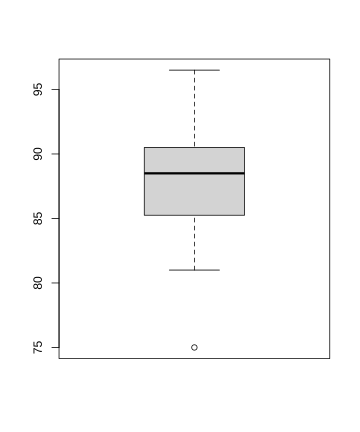
\includegraphics[width=.49\linewidth]{bookdownproj_files/figure-latex/unnamed-chunk-14-1} \end{center}
\vfill
\columnbreak
\vfill
\[ P(-t_{df})= 1 - P(t_{df}) \]
\vfill
\end{multicols}

\begin{table}[!h]
\centering
\resizebox{\linewidth}{!}{
\begin{tabular}{>{}r|rrrrrrrrrrrrrrr}
\toprule
\multicolumn{1}{c}{ } & \multicolumn{15}{c}{Fläche} \\
\cmidrule(l{3pt}r{3pt}){2-16}
$df$ & 0,55 & 0,6 & 0,65 & 0,7 & 0,75 & 0,8 & 0,85 & 0,9 & 0,95 & 0,975 & 0,99 & 0,995 & 0,999 & 0,9995 & 0,9999\\
\midrule
\cellcolor{gray!6}{1} & \cellcolor{gray!6}{0,158} & \cellcolor{gray!6}{0,325} & \cellcolor{gray!6}{0,510} & \cellcolor{gray!6}{0,727} & \cellcolor{gray!6}{1,000} & \cellcolor{gray!6}{1,376} & \cellcolor{gray!6}{1,963} & \cellcolor{gray!6}{3,078} & \cellcolor{gray!6}{6,314} & \cellcolor{gray!6}{12,706} & \cellcolor{gray!6}{31,821} & \cellcolor{gray!6}{63,657} & \cellcolor{gray!6}{318,309} & \cellcolor{gray!6}{636,619} & \cellcolor{gray!6}{3183,099}\\
2 & 0,142 & 0,289 & 0,445 & 0,617 & 0,816 & 1,061 & 1,386 & 1,886 & 2,920 & 4,303 & 6,965 & 9,925 & 22,327 & 31,599 & 70,700\\
\cellcolor{gray!6}{3} & \cellcolor{gray!6}{0,137} & \cellcolor{gray!6}{0,277} & \cellcolor{gray!6}{0,424} & \cellcolor{gray!6}{0,584} & \cellcolor{gray!6}{0,765} & \cellcolor{gray!6}{0,978} & \cellcolor{gray!6}{1,250} & \cellcolor{gray!6}{1,638} & \cellcolor{gray!6}{2,353} & \cellcolor{gray!6}{3,182} & \cellcolor{gray!6}{4,541} & \cellcolor{gray!6}{5,841} & \cellcolor{gray!6}{10,215} & \cellcolor{gray!6}{12,924} & \cellcolor{gray!6}{22,204}\\
4 & 0,134 & 0,271 & 0,414 & 0,569 & 0,741 & 0,941 & 1,190 & 1,533 & 2,132 & 2,776 & 3,747 & 4,604 & 7,173 & 8,610 & 13,034\\
\cellcolor{gray!6}{5} & \cellcolor{gray!6}{0,132} & \cellcolor{gray!6}{0,267} & \cellcolor{gray!6}{0,408} & \cellcolor{gray!6}{0,559} & \cellcolor{gray!6}{0,727} & \cellcolor{gray!6}{0,920} & \cellcolor{gray!6}{1,156} & \cellcolor{gray!6}{1,476} & \cellcolor{gray!6}{2,015} & \cellcolor{gray!6}{2,571} & \cellcolor{gray!6}{3,365} & \cellcolor{gray!6}{4,032} & \cellcolor{gray!6}{5,893} & \cellcolor{gray!6}{6,869} & \cellcolor{gray!6}{9,678}\\
\addlinespace
6 & 0,131 & 0,265 & 0,404 & 0,553 & 0,718 & 0,906 & 1,134 & 1,440 & 1,943 & 2,447 & 3,143 & 3,707 & 5,208 & 5,959 & 8,025\\
\cellcolor{gray!6}{7} & \cellcolor{gray!6}{0,130} & \cellcolor{gray!6}{0,263} & \cellcolor{gray!6}{0,402} & \cellcolor{gray!6}{0,549} & \cellcolor{gray!6}{0,711} & \cellcolor{gray!6}{0,896} & \cellcolor{gray!6}{1,119} & \cellcolor{gray!6}{1,415} & \cellcolor{gray!6}{1,895} & \cellcolor{gray!6}{2,365} & \cellcolor{gray!6}{2,998} & \cellcolor{gray!6}{3,499} & \cellcolor{gray!6}{4,785} & \cellcolor{gray!6}{5,408} & \cellcolor{gray!6}{7,063}\\
8 & 0,130 & 0,262 & 0,399 & 0,546 & 0,706 & 0,889 & 1,108 & 1,397 & 1,860 & 2,306 & 2,896 & 3,355 & 4,501 & 5,041 & 6,442\\
\cellcolor{gray!6}{9} & \cellcolor{gray!6}{0,129} & \cellcolor{gray!6}{0,261} & \cellcolor{gray!6}{0,398} & \cellcolor{gray!6}{0,543} & \cellcolor{gray!6}{0,703} & \cellcolor{gray!6}{0,883} & \cellcolor{gray!6}{1,100} & \cellcolor{gray!6}{1,383} & \cellcolor{gray!6}{1,833} & \cellcolor{gray!6}{2,262} & \cellcolor{gray!6}{2,821} & \cellcolor{gray!6}{3,250} & \cellcolor{gray!6}{4,297} & \cellcolor{gray!6}{4,781} & \cellcolor{gray!6}{6,010}\\
10 & 0,129 & 0,260 & 0,397 & 0,542 & 0,700 & 0,879 & 1,093 & 1,372 & 1,812 & 2,228 & 2,764 & 3,169 & 4,144 & 4,587 & 5,694\\
\addlinespace
\cellcolor{gray!6}{11} & \cellcolor{gray!6}{0,129} & \cellcolor{gray!6}{0,260} & \cellcolor{gray!6}{0,396} & \cellcolor{gray!6}{0,540} & \cellcolor{gray!6}{0,697} & \cellcolor{gray!6}{0,876} & \cellcolor{gray!6}{1,088} & \cellcolor{gray!6}{1,363} & \cellcolor{gray!6}{1,796} & \cellcolor{gray!6}{2,201} & \cellcolor{gray!6}{2,718} & \cellcolor{gray!6}{3,106} & \cellcolor{gray!6}{4,025} & \cellcolor{gray!6}{4,437} & \cellcolor{gray!6}{5,453}\\
12 & 0,128 & 0,259 & 0,395 & 0,539 & 0,695 & 0,873 & 1,083 & 1,356 & 1,782 & 2,179 & 2,681 & 3,055 & 3,930 & 4,318 & 5,263\\
\cellcolor{gray!6}{13} & \cellcolor{gray!6}{0,128} & \cellcolor{gray!6}{0,259} & \cellcolor{gray!6}{0,394} & \cellcolor{gray!6}{0,538} & \cellcolor{gray!6}{0,694} & \cellcolor{gray!6}{0,870} & \cellcolor{gray!6}{1,079} & \cellcolor{gray!6}{1,350} & \cellcolor{gray!6}{1,771} & \cellcolor{gray!6}{2,160} & \cellcolor{gray!6}{2,650} & \cellcolor{gray!6}{3,012} & \cellcolor{gray!6}{3,852} & \cellcolor{gray!6}{4,221} & \cellcolor{gray!6}{5,111}\\
14 & 0,128 & 0,258 & 0,393 & 0,537 & 0,692 & 0,868 & 1,076 & 1,345 & 1,761 & 2,145 & 2,624 & 2,977 & 3,787 & 4,140 & 4,985\\
\cellcolor{gray!6}{15} & \cellcolor{gray!6}{0,128} & \cellcolor{gray!6}{0,258} & \cellcolor{gray!6}{0,393} & \cellcolor{gray!6}{0,536} & \cellcolor{gray!6}{0,691} & \cellcolor{gray!6}{0,866} & \cellcolor{gray!6}{1,074} & \cellcolor{gray!6}{1,341} & \cellcolor{gray!6}{1,753} & \cellcolor{gray!6}{2,131} & \cellcolor{gray!6}{2,602} & \cellcolor{gray!6}{2,947} & \cellcolor{gray!6}{3,733} & \cellcolor{gray!6}{4,073} & \cellcolor{gray!6}{4,880}\\
\addlinespace
16 & 0,128 & 0,258 & 0,392 & 0,535 & 0,690 & 0,865 & 1,071 & 1,337 & 1,746 & 2,120 & 2,583 & 2,921 & 3,686 & 4,015 & 4,791\\
\cellcolor{gray!6}{17} & \cellcolor{gray!6}{0,128} & \cellcolor{gray!6}{0,257} & \cellcolor{gray!6}{0,392} & \cellcolor{gray!6}{0,534} & \cellcolor{gray!6}{0,689} & \cellcolor{gray!6}{0,863} & \cellcolor{gray!6}{1,069} & \cellcolor{gray!6}{1,333} & \cellcolor{gray!6}{1,740} & \cellcolor{gray!6}{2,110} & \cellcolor{gray!6}{2,567} & \cellcolor{gray!6}{2,898} & \cellcolor{gray!6}{3,646} & \cellcolor{gray!6}{3,965} & \cellcolor{gray!6}{4,714}\\
18 & 0,127 & 0,257 & 0,392 & 0,534 & 0,688 & 0,862 & 1,067 & 1,330 & 1,734 & 2,101 & 2,552 & 2,878 & 3,610 & 3,922 & 4,648\\
\cellcolor{gray!6}{19} & \cellcolor{gray!6}{0,127} & \cellcolor{gray!6}{0,257} & \cellcolor{gray!6}{0,391} & \cellcolor{gray!6}{0,533} & \cellcolor{gray!6}{0,688} & \cellcolor{gray!6}{0,861} & \cellcolor{gray!6}{1,066} & \cellcolor{gray!6}{1,328} & \cellcolor{gray!6}{1,729} & \cellcolor{gray!6}{2,093} & \cellcolor{gray!6}{2,539} & \cellcolor{gray!6}{2,861} & \cellcolor{gray!6}{3,579} & \cellcolor{gray!6}{3,883} & \cellcolor{gray!6}{4,590}\\
20 & 0,127 & 0,257 & 0,391 & 0,533 & 0,687 & 0,860 & 1,064 & 1,325 & 1,725 & 2,086 & 2,528 & 2,845 & 3,552 & 3,850 & 4,539\\
\addlinespace
\cellcolor{gray!6}{25} & \cellcolor{gray!6}{0,127} & \cellcolor{gray!6}{0,256} & \cellcolor{gray!6}{0,390} & \cellcolor{gray!6}{0,531} & \cellcolor{gray!6}{0,684} & \cellcolor{gray!6}{0,856} & \cellcolor{gray!6}{1,058} & \cellcolor{gray!6}{1,316} & \cellcolor{gray!6}{1,708} & \cellcolor{gray!6}{2,060} & \cellcolor{gray!6}{2,485} & \cellcolor{gray!6}{2,787} & \cellcolor{gray!6}{3,450} & \cellcolor{gray!6}{3,725} & \cellcolor{gray!6}{4,352}\\
30 & 0,127 & 0,256 & 0,389 & 0,530 & 0,683 & 0,854 & 1,055 & 1,310 & 1,697 & 2,042 & 2,457 & 2,750 & 3,385 & 3,646 & 4,234\\
\cellcolor{gray!6}{35} & \cellcolor{gray!6}{0,127} & \cellcolor{gray!6}{0,255} & \cellcolor{gray!6}{0,388} & \cellcolor{gray!6}{0,529} & \cellcolor{gray!6}{0,682} & \cellcolor{gray!6}{0,852} & \cellcolor{gray!6}{1,052} & \cellcolor{gray!6}{1,306} & \cellcolor{gray!6}{1,690} & \cellcolor{gray!6}{2,030} & \cellcolor{gray!6}{2,438} & \cellcolor{gray!6}{2,724} & \cellcolor{gray!6}{3,340} & \cellcolor{gray!6}{3,591} & \cellcolor{gray!6}{4,153}\\
40 & 0,126 & 0,255 & 0,388 & 0,529 & 0,681 & 0,851 & 1,050 & 1,303 & 1,684 & 2,021 & 2,423 & 2,704 & 3,307 & 3,551 & 4,094\\
\cellcolor{gray!6}{45} & \cellcolor{gray!6}{0,126} & \cellcolor{gray!6}{0,255} & \cellcolor{gray!6}{0,388} & \cellcolor{gray!6}{0,528} & \cellcolor{gray!6}{0,680} & \cellcolor{gray!6}{0,850} & \cellcolor{gray!6}{1,049} & \cellcolor{gray!6}{1,301} & \cellcolor{gray!6}{1,679} & \cellcolor{gray!6}{2,014} & \cellcolor{gray!6}{2,412} & \cellcolor{gray!6}{2,690} & \cellcolor{gray!6}{3,281} & \cellcolor{gray!6}{3,520} & \cellcolor{gray!6}{4,049}\\
\addlinespace
50 & 0,126 & 0,255 & 0,388 & 0,528 & 0,679 & 0,849 & 1,047 & 1,299 & 1,676 & 2,009 & 2,403 & 2,678 & 3,261 & 3,496 & 4,014\\
\cellcolor{gray!6}{55} & \cellcolor{gray!6}{0,126} & \cellcolor{gray!6}{0,255} & \cellcolor{gray!6}{0,387} & \cellcolor{gray!6}{0,527} & \cellcolor{gray!6}{0,679} & \cellcolor{gray!6}{0,848} & \cellcolor{gray!6}{1,046} & \cellcolor{gray!6}{1,297} & \cellcolor{gray!6}{1,673} & \cellcolor{gray!6}{2,004} & \cellcolor{gray!6}{2,396} & \cellcolor{gray!6}{2,668} & \cellcolor{gray!6}{3,245} & \cellcolor{gray!6}{3,476} & \cellcolor{gray!6}{3,986}\\
60 & 0,126 & 0,254 & 0,387 & 0,527 & 0,679 & 0,848 & 1,045 & 1,296 & 1,671 & 2,000 & 2,390 & 2,660 & 3,232 & 3,460 & 3,962\\
\cellcolor{gray!6}{65} & \cellcolor{gray!6}{0,126} & \cellcolor{gray!6}{0,254} & \cellcolor{gray!6}{0,387} & \cellcolor{gray!6}{0,527} & \cellcolor{gray!6}{0,678} & \cellcolor{gray!6}{0,847} & \cellcolor{gray!6}{1,045} & \cellcolor{gray!6}{1,295} & \cellcolor{gray!6}{1,669} & \cellcolor{gray!6}{1,997} & \cellcolor{gray!6}{2,385} & \cellcolor{gray!6}{2,654} & \cellcolor{gray!6}{3,220} & \cellcolor{gray!6}{3,447} & \cellcolor{gray!6}{3,942}\\
70 & 0,126 & 0,254 & 0,387 & 0,527 & 0,678 & 0,847 & 1,044 & 1,294 & 1,667 & 1,994 & 2,381 & 2,648 & 3,211 & 3,435 & 3,926\\
\addlinespace
\cellcolor{gray!6}{75} & \cellcolor{gray!6}{0,126} & \cellcolor{gray!6}{0,254} & \cellcolor{gray!6}{0,387} & \cellcolor{gray!6}{0,527} & \cellcolor{gray!6}{0,678} & \cellcolor{gray!6}{0,846} & \cellcolor{gray!6}{1,044} & \cellcolor{gray!6}{1,293} & \cellcolor{gray!6}{1,665} & \cellcolor{gray!6}{1,992} & \cellcolor{gray!6}{2,377} & \cellcolor{gray!6}{2,643} & \cellcolor{gray!6}{3,202} & \cellcolor{gray!6}{3,425} & \cellcolor{gray!6}{3,911}\\
80 & 0,126 & 0,254 & 0,387 & 0,526 & 0,678 & 0,846 & 1,043 & 1,292 & 1,664 & 1,990 & 2,374 & 2,639 & 3,195 & 3,416 & 3,899\\
\cellcolor{gray!6}{90} & \cellcolor{gray!6}{0,126} & \cellcolor{gray!6}{0,254} & \cellcolor{gray!6}{0,387} & \cellcolor{gray!6}{0,526} & \cellcolor{gray!6}{0,677} & \cellcolor{gray!6}{0,846} & \cellcolor{gray!6}{1,042} & \cellcolor{gray!6}{1,291} & \cellcolor{gray!6}{1,662} & \cellcolor{gray!6}{1,987} & \cellcolor{gray!6}{2,368} & \cellcolor{gray!6}{2,632} & \cellcolor{gray!6}{3,183} & \cellcolor{gray!6}{3,402} & \cellcolor{gray!6}{3,878}\\
100 & 0,126 & 0,254 & 0,386 & 0,526 & 0,677 & 0,845 & 1,042 & 1,290 & 1,660 & 1,984 & 2,364 & 2,626 & 3,174 & 3,390 & 3,862\\
\cellcolor{gray!6}{110} & \cellcolor{gray!6}{0,126} & \cellcolor{gray!6}{0,254} & \cellcolor{gray!6}{0,386} & \cellcolor{gray!6}{0,526} & \cellcolor{gray!6}{0,677} & \cellcolor{gray!6}{0,845} & \cellcolor{gray!6}{1,041} & \cellcolor{gray!6}{1,289} & \cellcolor{gray!6}{1,659} & \cellcolor{gray!6}{1,982} & \cellcolor{gray!6}{2,361} & \cellcolor{gray!6}{2,621} & \cellcolor{gray!6}{3,166} & \cellcolor{gray!6}{3,381} & \cellcolor{gray!6}{3,848}\\
\addlinespace
120 & 0,126 & 0,254 & 0,386 & 0,526 & 0,677 & 0,845 & 1,041 & 1,289 & 1,658 & 1,980 & 2,358 & 2,617 & 3,160 & 3,373 & 3,837\\
\cellcolor{gray!6}{130} & \cellcolor{gray!6}{0,126} & \cellcolor{gray!6}{0,254} & \cellcolor{gray!6}{0,386} & \cellcolor{gray!6}{0,526} & \cellcolor{gray!6}{0,676} & \cellcolor{gray!6}{0,844} & \cellcolor{gray!6}{1,041} & \cellcolor{gray!6}{1,288} & \cellcolor{gray!6}{1,657} & \cellcolor{gray!6}{1,978} & \cellcolor{gray!6}{2,355} & \cellcolor{gray!6}{2,614} & \cellcolor{gray!6}{3,154} & \cellcolor{gray!6}{3,367} & \cellcolor{gray!6}{3,828}\\
140 & 0,126 & 0,254 & 0,386 & 0,526 & 0,676 & 0,844 & 1,040 & 1,288 & 1,656 & 1,977 & 2,353 & 2,611 & 3,149 & 3,361 & 3,820\\
\cellcolor{gray!6}{150} & \cellcolor{gray!6}{0,126} & \cellcolor{gray!6}{0,254} & \cellcolor{gray!6}{0,386} & \cellcolor{gray!6}{0,526} & \cellcolor{gray!6}{0,676} & \cellcolor{gray!6}{0,844} & \cellcolor{gray!6}{1,040} & \cellcolor{gray!6}{1,287} & \cellcolor{gray!6}{1,655} & \cellcolor{gray!6}{1,976} & \cellcolor{gray!6}{2,351} & \cellcolor{gray!6}{2,609} & \cellcolor{gray!6}{3,145} & \cellcolor{gray!6}{3,357} & \cellcolor{gray!6}{3,813}\\
200 & 0,126 & 0,254 & 0,386 & 0,525 & 0,676 & 0,843 & 1,039 & 1,286 & 1,653 & 1,972 & 2,345 & 2,601 & 3,131 & 3,340 & 3,789\\
\addlinespace
\cellcolor{gray!6}{300} & \cellcolor{gray!6}{0,126} & \cellcolor{gray!6}{0,254} & \cellcolor{gray!6}{0,386} & \cellcolor{gray!6}{0,525} & \cellcolor{gray!6}{0,675} & \cellcolor{gray!6}{0,843} & \cellcolor{gray!6}{1,038} & \cellcolor{gray!6}{1,284} & \cellcolor{gray!6}{1,650} & \cellcolor{gray!6}{1,968} & \cellcolor{gray!6}{2,339} & \cellcolor{gray!6}{2,592} & \cellcolor{gray!6}{3,118} & \cellcolor{gray!6}{3,323} & \cellcolor{gray!6}{3,765}\\
400 & 0,126 & 0,254 & 0,386 & 0,525 & 0,675 & 0,843 & 1,038 & 1,284 & 1,649 & 1,966 & 2,336 & 2,588 & 3,111 & 3,315 & 3,754\\
\cellcolor{gray!6}{500} & \cellcolor{gray!6}{0,126} & \cellcolor{gray!6}{0,253} & \cellcolor{gray!6}{0,386} & \cellcolor{gray!6}{0,525} & \cellcolor{gray!6}{0,675} & \cellcolor{gray!6}{0,842} & \cellcolor{gray!6}{1,038} & \cellcolor{gray!6}{1,283} & \cellcolor{gray!6}{1,648} & \cellcolor{gray!6}{1,965} & \cellcolor{gray!6}{2,334} & \cellcolor{gray!6}{2,586} & \cellcolor{gray!6}{3,107} & \cellcolor{gray!6}{3,310} & \cellcolor{gray!6}{3,747}\\
1000 & 0,126 & 0,253 & 0,385 & 0,525 & 0,675 & 0,842 & 1,037 & 1,282 & 1,646 & 1,962 & 2,330 & 2,581 & 3,098 & 3,300 & 3,733\\
\cellcolor{gray!6}{$z$} & \cellcolor{gray!6}{0,126} & \cellcolor{gray!6}{0,253} & \cellcolor{gray!6}{0,385} & \cellcolor{gray!6}{0,524} & \cellcolor{gray!6}{0,674} & \cellcolor{gray!6}{0,842} & \cellcolor{gray!6}{1,036} & \cellcolor{gray!6}{1,282} & \cellcolor{gray!6}{1,645} & \cellcolor{gray!6}{1,960} & \cellcolor{gray!6}{2,326} & \cellcolor{gray!6}{2,576} & \cellcolor{gray!6}{3,090} & \cellcolor{gray!6}{3,291} & \cellcolor{gray!6}{3,719}\\
\bottomrule
\end{tabular}}
\end{table}

\pagebreak

\hypertarget{anhang-tabelle-f-verteilungen}{%
\subsection{Anhang: Tabelle F-Verteilungen}\label{anhang-tabelle-f-verteilungen}}

\begin{multicols}{2}


\begin{center}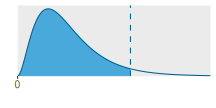
\includegraphics[width=.49\linewidth]{bookdownproj_files/figure-latex/unnamed-chunk-16-1} \end{center}

\[
F_{\textit{df}_1;\textit{df}_2;\alpha}=\frac{1}{F_{\textit{df}_2;\textit{df}_1;(1-\alpha)}} 
\]

\end{multicols}

\emph{Alle Werte für Flächenanteil 0,95}

\begin{table}[!h]
\centering
\resizebox{\linewidth}{!}{
\begin{tabular}{>{}r|rrrrrrrrrrrrrr}
\toprule
\multicolumn{1}{c}{ } & \multicolumn{14}{c}{$df_1$} \\
\cmidrule(l{3pt}r{3pt}){2-15}
$df_2$ &   1 &   2 &   3 &   4 &   5 &   6 &   7 &   8 &   9 &  10 &  15 &  20 &  50 & 100\\
\midrule
\cellcolor{gray!6}{1} & \cellcolor{gray!6}{161,45} & \cellcolor{gray!6}{199,50} & \cellcolor{gray!6}{215,71} & \cellcolor{gray!6}{224,58} & \cellcolor{gray!6}{230,16} & \cellcolor{gray!6}{233,99} & \cellcolor{gray!6}{236,77} & \cellcolor{gray!6}{238,88} & \cellcolor{gray!6}{240,54} & \cellcolor{gray!6}{241,88} & \cellcolor{gray!6}{245,95} & \cellcolor{gray!6}{248,01} & \cellcolor{gray!6}{251,77} & \cellcolor{gray!6}{253,04}\\
2 & 18,51 & 19,00 & 19,16 & 19,25 & 19,30 & 19,33 & 19,35 & 19,37 & 19,38 & 19,40 & 19,43 & 19,45 & 19,48 & 19,49\\
\cellcolor{gray!6}{3} & \cellcolor{gray!6}{10,13} & \cellcolor{gray!6}{9,55} & \cellcolor{gray!6}{9,28} & \cellcolor{gray!6}{9,12} & \cellcolor{gray!6}{9,01} & \cellcolor{gray!6}{8,94} & \cellcolor{gray!6}{8,89} & \cellcolor{gray!6}{8,85} & \cellcolor{gray!6}{8,81} & \cellcolor{gray!6}{8,79} & \cellcolor{gray!6}{8,70} & \cellcolor{gray!6}{8,66} & \cellcolor{gray!6}{8,58} & \cellcolor{gray!6}{8,55}\\
4 & 7,71 & 6,94 & 6,59 & 6,39 & 6,26 & 6,16 & 6,09 & 6,04 & 6,00 & 5,96 & 5,86 & 5,80 & 5,70 & 5,66\\
\cellcolor{gray!6}{5} & \cellcolor{gray!6}{6,61} & \cellcolor{gray!6}{5,79} & \cellcolor{gray!6}{5,41} & \cellcolor{gray!6}{5,19} & \cellcolor{gray!6}{5,05} & \cellcolor{gray!6}{4,95} & \cellcolor{gray!6}{4,88} & \cellcolor{gray!6}{4,82} & \cellcolor{gray!6}{4,77} & \cellcolor{gray!6}{4,74} & \cellcolor{gray!6}{4,62} & \cellcolor{gray!6}{4,56} & \cellcolor{gray!6}{4,44} & \cellcolor{gray!6}{4,41}\\
\addlinespace
6 & 5,99 & 5,14 & 4,76 & 4,53 & 4,39 & 4,28 & 4,21 & 4,15 & 4,10 & 4,06 & 3,94 & 3,87 & 3,75 & 3,71\\
\cellcolor{gray!6}{7} & \cellcolor{gray!6}{5,59} & \cellcolor{gray!6}{4,74} & \cellcolor{gray!6}{4,35} & \cellcolor{gray!6}{4,12} & \cellcolor{gray!6}{3,97} & \cellcolor{gray!6}{3,87} & \cellcolor{gray!6}{3,79} & \cellcolor{gray!6}{3,73} & \cellcolor{gray!6}{3,68} & \cellcolor{gray!6}{3,64} & \cellcolor{gray!6}{3,51} & \cellcolor{gray!6}{3,44} & \cellcolor{gray!6}{3,32} & \cellcolor{gray!6}{3,27}\\
8 & 5,32 & 4,46 & 4,07 & 3,84 & 3,69 & 3,58 & 3,50 & 3,44 & 3,39 & 3,35 & 3,22 & 3,15 & 3,02 & 2,97\\
\cellcolor{gray!6}{9} & \cellcolor{gray!6}{5,12} & \cellcolor{gray!6}{4,26} & \cellcolor{gray!6}{3,86} & \cellcolor{gray!6}{3,63} & \cellcolor{gray!6}{3,48} & \cellcolor{gray!6}{3,37} & \cellcolor{gray!6}{3,29} & \cellcolor{gray!6}{3,23} & \cellcolor{gray!6}{3,18} & \cellcolor{gray!6}{3,14} & \cellcolor{gray!6}{3,01} & \cellcolor{gray!6}{2,94} & \cellcolor{gray!6}{2,80} & \cellcolor{gray!6}{2,76}\\
10 & 4,96 & 4,10 & 3,71 & 3,48 & 3,33 & 3,22 & 3,14 & 3,07 & 3,02 & 2,98 & 2,85 & 2,77 & 2,64 & 2,59\\
\addlinespace
\cellcolor{gray!6}{11} & \cellcolor{gray!6}{4,84} & \cellcolor{gray!6}{3,98} & \cellcolor{gray!6}{3,59} & \cellcolor{gray!6}{3,36} & \cellcolor{gray!6}{3,20} & \cellcolor{gray!6}{3,09} & \cellcolor{gray!6}{3,01} & \cellcolor{gray!6}{2,95} & \cellcolor{gray!6}{2,90} & \cellcolor{gray!6}{2,85} & \cellcolor{gray!6}{2,72} & \cellcolor{gray!6}{2,65} & \cellcolor{gray!6}{2,51} & \cellcolor{gray!6}{2,46}\\
12 & 4,75 & 3,89 & 3,49 & 3,26 & 3,11 & 3,00 & 2,91 & 2,85 & 2,80 & 2,75 & 2,62 & 2,54 & 2,40 & 2,35\\
\cellcolor{gray!6}{13} & \cellcolor{gray!6}{4,67} & \cellcolor{gray!6}{3,81} & \cellcolor{gray!6}{3,41} & \cellcolor{gray!6}{3,18} & \cellcolor{gray!6}{3,03} & \cellcolor{gray!6}{2,92} & \cellcolor{gray!6}{2,83} & \cellcolor{gray!6}{2,77} & \cellcolor{gray!6}{2,71} & \cellcolor{gray!6}{2,67} & \cellcolor{gray!6}{2,53} & \cellcolor{gray!6}{2,46} & \cellcolor{gray!6}{2,31} & \cellcolor{gray!6}{2,26}\\
14 & 4,60 & 3,74 & 3,34 & 3,11 & 2,96 & 2,85 & 2,76 & 2,70 & 2,65 & 2,60 & 2,46 & 2,39 & 2,24 & 2,19\\
\cellcolor{gray!6}{15} & \cellcolor{gray!6}{4,54} & \cellcolor{gray!6}{3,68} & \cellcolor{gray!6}{3,29} & \cellcolor{gray!6}{3,06} & \cellcolor{gray!6}{2,90} & \cellcolor{gray!6}{2,79} & \cellcolor{gray!6}{2,71} & \cellcolor{gray!6}{2,64} & \cellcolor{gray!6}{2,59} & \cellcolor{gray!6}{2,54} & \cellcolor{gray!6}{2,40} & \cellcolor{gray!6}{2,33} & \cellcolor{gray!6}{2,18} & \cellcolor{gray!6}{2,12}\\
\addlinespace
16 & 4,49 & 3,63 & 3,24 & 3,01 & 2,85 & 2,74 & 2,66 & 2,59 & 2,54 & 2,49 & 2,35 & 2,28 & 2,12 & 2,07\\
\cellcolor{gray!6}{17} & \cellcolor{gray!6}{4,45} & \cellcolor{gray!6}{3,59} & \cellcolor{gray!6}{3,20} & \cellcolor{gray!6}{2,96} & \cellcolor{gray!6}{2,81} & \cellcolor{gray!6}{2,70} & \cellcolor{gray!6}{2,61} & \cellcolor{gray!6}{2,55} & \cellcolor{gray!6}{2,49} & \cellcolor{gray!6}{2,45} & \cellcolor{gray!6}{2,31} & \cellcolor{gray!6}{2,23} & \cellcolor{gray!6}{2,08} & \cellcolor{gray!6}{2,02}\\
18 & 4,41 & 3,55 & 3,16 & 2,93 & 2,77 & 2,66 & 2,58 & 2,51 & 2,46 & 2,41 & 2,27 & 2,19 & 2,04 & 1,98\\
\cellcolor{gray!6}{19} & \cellcolor{gray!6}{4,38} & \cellcolor{gray!6}{3,52} & \cellcolor{gray!6}{3,13} & \cellcolor{gray!6}{2,90} & \cellcolor{gray!6}{2,74} & \cellcolor{gray!6}{2,63} & \cellcolor{gray!6}{2,54} & \cellcolor{gray!6}{2,48} & \cellcolor{gray!6}{2,42} & \cellcolor{gray!6}{2,38} & \cellcolor{gray!6}{2,23} & \cellcolor{gray!6}{2,16} & \cellcolor{gray!6}{2,00} & \cellcolor{gray!6}{1,94}\\
20 & 4,35 & 3,49 & 3,10 & 2,87 & 2,71 & 2,60 & 2,51 & 2,45 & 2,39 & 2,35 & 2,20 & 2,12 & 1,97 & 1,91\\
\addlinespace
\cellcolor{gray!6}{25} & \cellcolor{gray!6}{4,24} & \cellcolor{gray!6}{3,39} & \cellcolor{gray!6}{2,99} & \cellcolor{gray!6}{2,76} & \cellcolor{gray!6}{2,60} & \cellcolor{gray!6}{2,49} & \cellcolor{gray!6}{2,40} & \cellcolor{gray!6}{2,34} & \cellcolor{gray!6}{2,28} & \cellcolor{gray!6}{2,24} & \cellcolor{gray!6}{2,09} & \cellcolor{gray!6}{2,01} & \cellcolor{gray!6}{1,84} & \cellcolor{gray!6}{1,78}\\
30 & 4,17 & 3,32 & 2,92 & 2,69 & 2,53 & 2,42 & 2,33 & 2,27 & 2,21 & 2,16 & 2,01 & 1,93 & 1,76 & 1,70\\
\cellcolor{gray!6}{35} & \cellcolor{gray!6}{4,12} & \cellcolor{gray!6}{3,27} & \cellcolor{gray!6}{2,87} & \cellcolor{gray!6}{2,64} & \cellcolor{gray!6}{2,49} & \cellcolor{gray!6}{2,37} & \cellcolor{gray!6}{2,29} & \cellcolor{gray!6}{2,22} & \cellcolor{gray!6}{2,16} & \cellcolor{gray!6}{2,11} & \cellcolor{gray!6}{1,96} & \cellcolor{gray!6}{1,88} & \cellcolor{gray!6}{1,70} & \cellcolor{gray!6}{1,63}\\
40 & 4,08 & 3,23 & 2,84 & 2,61 & 2,45 & 2,34 & 2,25 & 2,18 & 2,12 & 2,08 & 1,92 & 1,84 & 1,66 & 1,59\\
\cellcolor{gray!6}{45} & \cellcolor{gray!6}{4,06} & \cellcolor{gray!6}{3,20} & \cellcolor{gray!6}{2,81} & \cellcolor{gray!6}{2,58} & \cellcolor{gray!6}{2,42} & \cellcolor{gray!6}{2,31} & \cellcolor{gray!6}{2,22} & \cellcolor{gray!6}{2,15} & \cellcolor{gray!6}{2,10} & \cellcolor{gray!6}{2,05} & \cellcolor{gray!6}{1,89} & \cellcolor{gray!6}{1,81} & \cellcolor{gray!6}{1,63} & \cellcolor{gray!6}{1,55}\\
\addlinespace
50 & 4,03 & 3,18 & 2,79 & 2,56 & 2,40 & 2,29 & 2,20 & 2,13 & 2,07 & 2,03 & 1,87 & 1,78 & 1,60 & 1,52\\
\cellcolor{gray!6}{60} & \cellcolor{gray!6}{4,00} & \cellcolor{gray!6}{3,15} & \cellcolor{gray!6}{2,76} & \cellcolor{gray!6}{2,53} & \cellcolor{gray!6}{2,37} & \cellcolor{gray!6}{2,25} & \cellcolor{gray!6}{2,17} & \cellcolor{gray!6}{2,10} & \cellcolor{gray!6}{2,04} & \cellcolor{gray!6}{1,99} & \cellcolor{gray!6}{1,84} & \cellcolor{gray!6}{1,75} & \cellcolor{gray!6}{1,56} & \cellcolor{gray!6}{1,48}\\
70 & 3,98 & 3,13 & 2,74 & 2,50 & 2,35 & 2,23 & 2,14 & 2,07 & 2,02 & 1,97 & 1,81 & 1,72 & 1,53 & 1,45\\
\cellcolor{gray!6}{80} & \cellcolor{gray!6}{3,96} & \cellcolor{gray!6}{3,11} & \cellcolor{gray!6}{2,72} & \cellcolor{gray!6}{2,49} & \cellcolor{gray!6}{2,33} & \cellcolor{gray!6}{2,21} & \cellcolor{gray!6}{2,13} & \cellcolor{gray!6}{2,06} & \cellcolor{gray!6}{2,00} & \cellcolor{gray!6}{1,95} & \cellcolor{gray!6}{1,79} & \cellcolor{gray!6}{1,70} & \cellcolor{gray!6}{1,51} & \cellcolor{gray!6}{1,43}\\
90 & 3,95 & 3,10 & 2,71 & 2,47 & 2,32 & 2,20 & 2,11 & 2,04 & 1,99 & 1,94 & 1,78 & 1,69 & 1,49 & 1,41\\
\addlinespace
\cellcolor{gray!6}{100} & \cellcolor{gray!6}{3,94} & \cellcolor{gray!6}{3,09} & \cellcolor{gray!6}{2,70} & \cellcolor{gray!6}{2,46} & \cellcolor{gray!6}{2,31} & \cellcolor{gray!6}{2,19} & \cellcolor{gray!6}{2,10} & \cellcolor{gray!6}{2,03} & \cellcolor{gray!6}{1,97} & \cellcolor{gray!6}{1,93} & \cellcolor{gray!6}{1,77} & \cellcolor{gray!6}{1,68} & \cellcolor{gray!6}{1,48} & \cellcolor{gray!6}{1,39}\\
110 & 3,93 & 3,08 & 2,69 & 2,45 & 2,30 & 2,18 & 2,09 & 2,02 & 1,97 & 1,92 & 1,76 & 1,67 & 1,47 & 1,38\\
\cellcolor{gray!6}{120} & \cellcolor{gray!6}{3,92} & \cellcolor{gray!6}{3,07} & \cellcolor{gray!6}{2,68} & \cellcolor{gray!6}{2,45} & \cellcolor{gray!6}{2,29} & \cellcolor{gray!6}{2,18} & \cellcolor{gray!6}{2,09} & \cellcolor{gray!6}{2,02} & \cellcolor{gray!6}{1,96} & \cellcolor{gray!6}{1,91} & \cellcolor{gray!6}{1,75} & \cellcolor{gray!6}{1,66} & \cellcolor{gray!6}{1,46} & \cellcolor{gray!6}{1,37}\\
130 & 3,91 & 3,07 & 2,67 & 2,44 & 2,28 & 2,17 & 2,08 & 2,01 & 1,95 & 1,90 & 1,74 & 1,65 & 1,45 & 1,36\\
\cellcolor{gray!6}{140} & \cellcolor{gray!6}{3,91} & \cellcolor{gray!6}{3,06} & \cellcolor{gray!6}{2,67} & \cellcolor{gray!6}{2,44} & \cellcolor{gray!6}{2,28} & \cellcolor{gray!6}{2,16} & \cellcolor{gray!6}{2,08} & \cellcolor{gray!6}{2,01} & \cellcolor{gray!6}{1,95} & \cellcolor{gray!6}{1,90} & \cellcolor{gray!6}{1,74} & \cellcolor{gray!6}{1,65} & \cellcolor{gray!6}{1,44} & \cellcolor{gray!6}{1,35}\\
\addlinespace
150 & 3,90 & 3,06 & 2,66 & 2,43 & 2,27 & 2,16 & 2,07 & 2,00 & 1,94 & 1,89 & 1,73 & 1,64 & 1,44 & 1,34\\
\cellcolor{gray!6}{200} & \cellcolor{gray!6}{3,89} & \cellcolor{gray!6}{3,04} & \cellcolor{gray!6}{2,65} & \cellcolor{gray!6}{2,42} & \cellcolor{gray!6}{2,26} & \cellcolor{gray!6}{2,14} & \cellcolor{gray!6}{2,06} & \cellcolor{gray!6}{1,98} & \cellcolor{gray!6}{1,93} & \cellcolor{gray!6}{1,88} & \cellcolor{gray!6}{1,72} & \cellcolor{gray!6}{1,62} & \cellcolor{gray!6}{1,41} & \cellcolor{gray!6}{1,32}\\
300 & 3,87 & 3,03 & 2,63 & 2,40 & 2,24 & 2,13 & 2,04 & 1,97 & 1,91 & 1,86 & 1,70 & 1,61 & 1,39 & 1,30\\
\cellcolor{gray!6}{400} & \cellcolor{gray!6}{3,86} & \cellcolor{gray!6}{3,02} & \cellcolor{gray!6}{2,63} & \cellcolor{gray!6}{2,39} & \cellcolor{gray!6}{2,24} & \cellcolor{gray!6}{2,12} & \cellcolor{gray!6}{2,03} & \cellcolor{gray!6}{1,96} & \cellcolor{gray!6}{1,90} & \cellcolor{gray!6}{1,85} & \cellcolor{gray!6}{1,69} & \cellcolor{gray!6}{1,60} & \cellcolor{gray!6}{1,38} & \cellcolor{gray!6}{1,28}\\
500 & 3,86 & 3,01 & 2,62 & 2,39 & 2,23 & 2,12 & 2,03 & 1,96 & 1,90 & 1,85 & 1,69 & 1,59 & 1,38 & 1,28\\
\addlinespace
\cellcolor{gray!6}{1000} & \cellcolor{gray!6}{3,85} & \cellcolor{gray!6}{3,00} & \cellcolor{gray!6}{2,61} & \cellcolor{gray!6}{2,38} & \cellcolor{gray!6}{2,22} & \cellcolor{gray!6}{2,11} & \cellcolor{gray!6}{2,02} & \cellcolor{gray!6}{1,95} & \cellcolor{gray!6}{1,89} & \cellcolor{gray!6}{1,84} & \cellcolor{gray!6}{1,68} & \cellcolor{gray!6}{1,58} & \cellcolor{gray!6}{1,36} & \cellcolor{gray!6}{1,26}\\
\bottomrule
\end{tabular}}
\end{table}

\pagebreak

\hypertarget{quellen-5}{%
\subsection{Quellen}\label{quellen-5}}

\hypertarget{korrelation}{%
\section{Korrelation}\label{korrelation}}

\hypertarget{lernziele-dieser-sitzung-6}{%
\subsection{Lernziele dieser Sitzung}\label{lernziele-dieser-sitzung-6}}

Sie können\ldots{}

\begin{itemize}
\tightlist
\item
  ein Streudiagramm interpretieren.
\item
  die Kovarianz von zwei Variablen berechnen.
\item
  den Korrelationskoeffizienten von zwei Variablen berechnen.
\end{itemize}

\hypertarget{bivariate-statistik}{%
\subsection{Bivariate Statistik}\label{bivariate-statistik}}

Grundlage der bivariaten Statistik ist es, dass für eine Reihe von Untersuchungsheinheiten jeweils zwei Merkmale erfasst sind.

Diese Merkmale werden üblicherweise mit \(x\) und \(y\) gekennzeichnet. Für jedes \(i\) (laufende Nummer der Merkmalsträger*innen) gibt es dann ein \(x_i\) (Ausprägung des Merkmals \(x\)) und ein \(y_i\) (Ausprägung des Merkmals \(y\)).

Das Streudiagramm (engl. \emph{scatter plot}) stellt alle erfassten Werte dar, indem es die Untersuchungseinheiten als Punkte arrangiert -- und zwar anhand ihres jeweiligen Werts der Variable \(x\) entlang der \(x\)-Achse und entlang der \(y\)-Achse anhand des \(y\)-Werts (s. \autoref{fig:scatter}).

\hypertarget{beispiel-23}{%
\subsubsection{Beispiel}\label{beispiel-23}}

Die statistischen Verfahren dieser Sitzung sollen wieder an einem Beispiel illustriert werden.

Wir fragen uns, ob der jährliche Ertrag in einem bestimmten Anbaugebiet für Klebreis in Nordostthailand mit dem jährlichen Niederschlag zusammenhängt. Die erfassten Werte sind in \autoref{tab:reis} festgehalten (``Rai'' ist ein \href{https://de.wikipedia.org/wiki/Rai_(Einheit)}{in Thailand übliches Flächenmaß}).

\begin{table}

\caption{\label{tab:unnamed-chunk-18}\label{tab:reis}Niederschlag und Ertrag im Reisanbau}
\centering
\begin{tabular}[t]{rrrr}
\toprule
\multicolumn{1}{c}{Laufende Nr.} & \multicolumn{1}{c}{Jahr} & \multicolumn{1}{c}{Niederschlag (mm)} & \multicolumn{1}{c}{Ertrag (kg/Rai)} \\
\cmidrule(l{3pt}r{3pt}){1-1} \cmidrule(l{3pt}r{3pt}){2-2} \cmidrule(l{3pt}r{3pt}){3-3} \cmidrule(l{3pt}r{3pt}){4-4}
$i$ &  & $x_i$ & $y_i$\\
\midrule
1 & 2008 & 1449 & 1860\\
2 & 2009 & 1472 & 2118\\
3 & 2010 & 1607 & 2225\\
4 & 2011 & 1494 & 2172\\
5 & 2012 & 1390 & 1816\\
6 & 2013 & 1764 & 2430\\
7 & 2014 & 1767 & 2580\\
8 & 2015 & 1765 & 2563\\
9 & 2016 & 1671 & 2276\\
10 & 2017 & 1838 & 2455\\
\bottomrule
\end{tabular}
\end{table}

In einem Streudiagramm können diese Werte veranschaulicht werden. Dabei ist es üblich, die unabhängige Variable auf der \(x\)-Achse und die abhängige Variable auf der \(y\)-Achse einzutragen. Im Beispiel liegt nahe, dass der Ertrag vom Regen abhängt, und nicht etwa umgekehrt.

\autoref{fig:scatter} ist das Streudiagramm für unser Beispiel. Es fällt schon rein optisch auf, dass ein Zusammenhang zu bestehen scheint: Je mehr Regen, desto reicher die Ernte. Doch wie lässt sich dieser Zusammenhang beziffern?

\begin{figure}[h]

{\centering 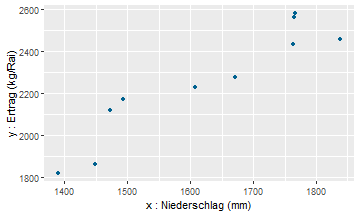
\includegraphics[width=.49\linewidth]{bookdownproj_files/figure-latex/scatter-1} 

}

\caption{Streudiagramm zum Reisanbau}\label{fig:scatter}
\end{figure}

\hypertarget{kovarianz}{%
\subsection{Kovarianz}\label{kovarianz}}

Die Kovarianz (engl. \emph{covariance}) \(s_{xy}\) gibt an, inwiefern die beiden Variablen \(x\) und \(y\) \emph{gemeinsam variieren}. Die Kovarianz ergibt sich durch die Summe der jeweiligen Produkte der Differenzen zu den Mittelwerten \((x_i-\bar{x})\) und \((y_i-\bar{y})\), geteilt durch \((n-1)\). Die Formel lautet also:

\[
s_{xy}=\frac{\sum\limits^n_{i=1}(x_i-\bar{x})\cdot(y_i-\bar{y})}{n-1}
\]\{\#eq:cov\}

\autoref{eq:cov} lässt erahnen: Wenn sowohl \(x\) als auch \(y\) in die gleiche Richtung vom jeweiligen Mittelwert abweichen (also beide Differenzen positiv oder beide Differenzen negativ), dann ist das Produkt positiv, sonst ist es negativ. Eine positive Kovarianz lässt also auf einen positiven Zusammenhang schließen (je größer \(x\), desto größer auch \(y\)), eine negative Kovarianz auf einen negativen Zusammenhang (je größer \(x\), desto \emph{kleiner} \(y\)).

\begin{rtip}
Der Befehl {\tt cov()} berechnet die Kovarianz einer bivariaten Verteilung in R.
\end{rtip}

\hypertarget{beispiel-24}{%
\subsubsection{Beispiel}\label{beispiel-24}}

Es macht Sinn, eine Tabelle anzulgen, in der Teilrechenschritte durchgeführt werden. \autoref{tab:ricemath} veranschaulicht dies.

\begin{table}

\caption{\label{tab:unnamed-chunk-19}\label{tab:ricemath}Hilfstabelle für die Berechnung der Kovarianz}
\centering
\begin{tabular}[t]{rrrrrr}
\toprule
$i$ & $x_i$ & $y_i$ & $(x_i-\bar{x})$ & $(y_i-\bar{y})$ & $(x_i-\bar{x})\cdot(y_i-\bar{y})$\\
\midrule
1 & 1449 & 1860 & -172,7 & -389,5 & 67266,65\\
2 & 1472 & 2118 & -149,7 & -131,5 & 19685,55\\
3 & 1607 & 2225 & -14,7 & -24,5 & 360,15\\
4 & 1494 & 2172 & -127,7 & -77,5 & 9896,75\\
5 & 1390 & 1816 & -231,7 & -433,5 & 100441,95\\
6 & 1764 & 2430 & 142,3 & 180,5 & 25685,15\\
7 & 1767 & 2580 & 145,3 & 330,5 & 48021,65\\
8 & 1765 & 2563 & 143,3 & 313,5 & 44924,55\\
9 & 1671 & 2276 & 49,3 & 26,5 & 1306,45\\
10 & 1838 & 2455 & 216,3 & 205,5 & 44449,65\\
\midrule
\textbf{Summe:} & \textbf{16217} & \textbf{22495} & \textbf{} & \textbf{} & \textbf{362038,5}\\
\bottomrule
\end{tabular}
\end{table}

Als Zwischenschritt müssen die Mittelwerte \(\bar{x}\) und \(\bar{y}\) berechnet werden, wofür die Summen der ersten beiden Spalten herangezogen werden können:

\[
\begin{aligned}
\bar{x}&=\frac{\sum\limits^n_{i=1}x_i}{n}\\[5pt]
       &=\frac{16217}{10}=1621,7\\[6pt]
\bar{y}&=\frac{\sum\limits^n_{i=1}y_i}{n}\\[5pt]
       &=\frac{22495}{10}=2249,5
\end{aligned}
\]

Schließlich ergibt Einsetzen der Produktsumme in \autoref{eq:cov} die Kovarianz:

\[\begin{aligned}
s_{xy}&=\frac{\sum\limits^n_{i=1}(x_i-\bar{x})\cdot(y_i-\bar{y})}{n-1}\\[5pt]
&\approx\frac{362038,5}{9}=40226,5
\end{aligned}\]

Die Kovarianz ist also \(s_{xy}=40226,5\). Was sagt uns diese Zahl? Zunächst ist sie positiv, womit wir von einer positiven Korrelation (je mehr Regen, desto mehr Ertrag) ausgehen können. Sie ist auch ``irgendwie'' ziemlich groß, was einen deutlichen Zusammenhang nahelegt. Aber die Kovarianz ist abhängig vom Maßstab -- wäre der Ertrag nicht in Kilogramm pro Rai, sondern (wie in Deutschland üblich) in Dezitonnen pro Hektar angegeben, dann wäre die Zahl deutlich kleiner (2514,156 um genau zu sein). Wie lässt sich die Stärke der Korrelation also unabhängig von den Maßeinheiten angeben?

\hypertarget{korrelationskoeffizient}{%
\subsection{Korrelationskoeffizient}\label{korrelationskoeffizient}}

Der Korrelationskoeffizent \(r\) (auch Produkt-Moment-Korrelation, Bravais-Pearson-Korrelation, Pearsons \(r\), engl. \emph{correlation coefficient}) standardisiert die Kovarianz \(s_{xy}\) anhand der Standardabweichungen \(s_x\) und \(s_y\). Die Formel lautet:

\[
r=\frac{s_{xy}}{s_x\cdot s_y}
\]\{\#eq:cor\}

Durch diese Standardisierung kann der Korrelationskoeffizient nur noch Werte zwischen \(r=-1\) (perfekte negative Korrelation) und \(r=1\) (perfekte positive Korrelation) annehmen. Ein Korrelationskoeffizient nahe \(r=0\) bedeutet, dass es keinen Zusammenhang zwischen den Variablen \(x\) und \(y\) gibt (s. \autoref{fig:corrs}).

\begin{figure}[h]

{\centering 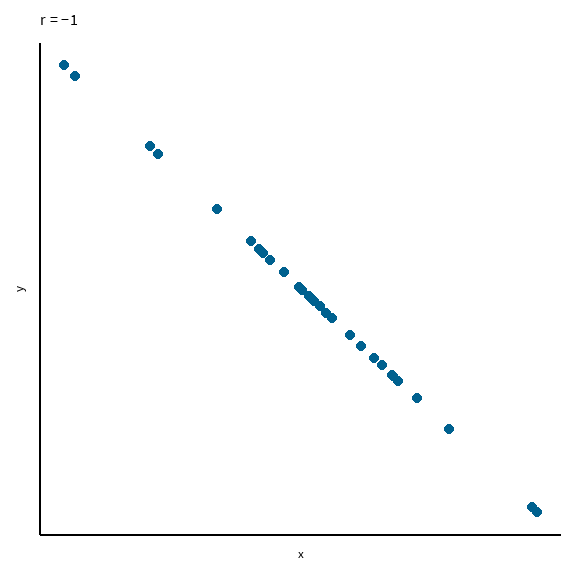
\includegraphics[width=.26\linewidth]{bookdownproj_files/figure-latex/corrs-1} 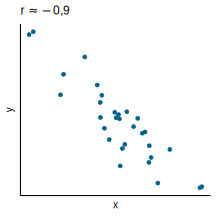
\includegraphics[width=.26\linewidth]{bookdownproj_files/figure-latex/corrs-2} 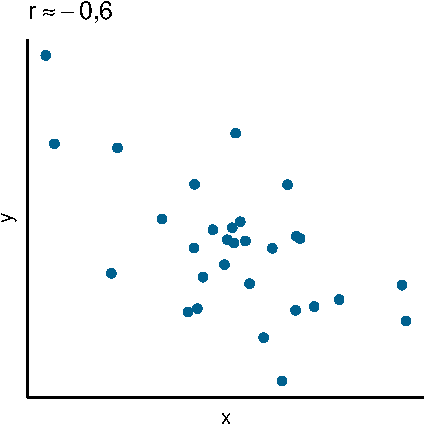
\includegraphics[width=.26\linewidth]{bookdownproj_files/figure-latex/corrs-3} 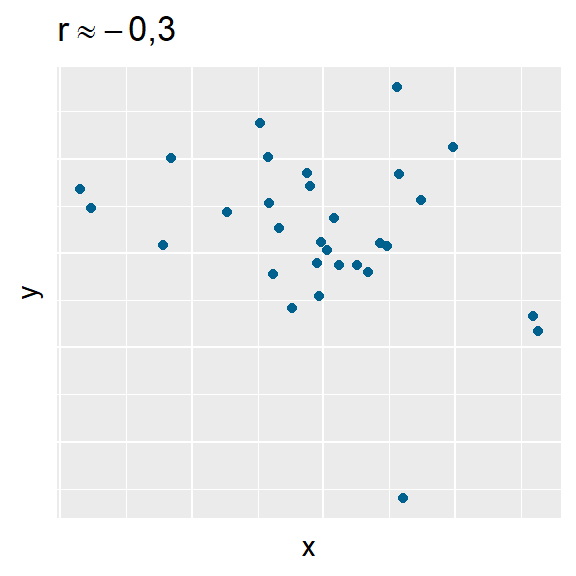
\includegraphics[width=.26\linewidth]{bookdownproj_files/figure-latex/corrs-4} 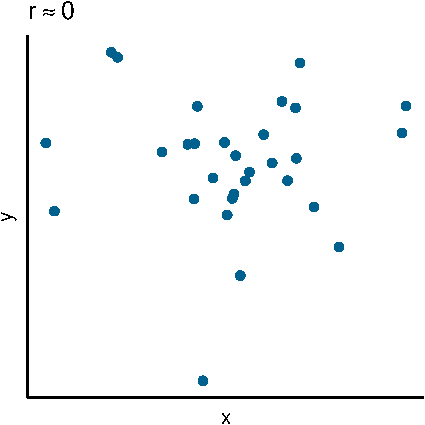
\includegraphics[width=.26\linewidth]{bookdownproj_files/figure-latex/corrs-5} 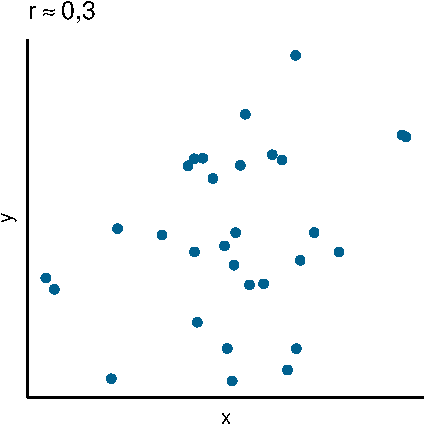
\includegraphics[width=.26\linewidth]{bookdownproj_files/figure-latex/corrs-6} 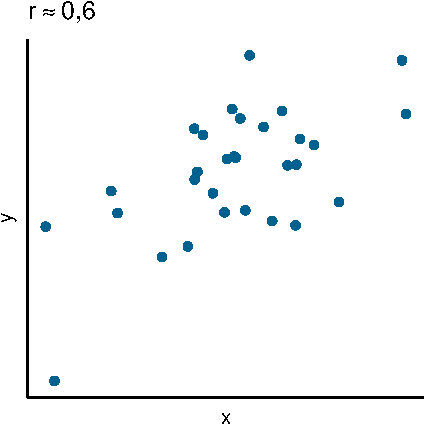
\includegraphics[width=.26\linewidth]{bookdownproj_files/figure-latex/corrs-7} 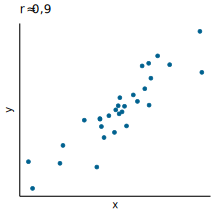
\includegraphics[width=.26\linewidth]{bookdownproj_files/figure-latex/corrs-8} 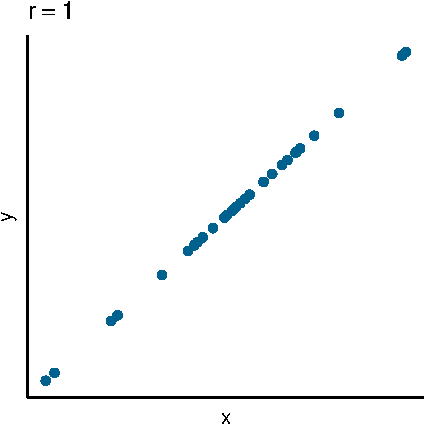
\includegraphics[width=.26\linewidth]{bookdownproj_files/figure-latex/corrs-9} 

}

\caption{Verschiedene Korrelationskoeffizienten}\label{fig:corrs}
\end{figure}

\begin{rtip}
In R kann der Korrelationskoeffizient von zwei Merkmalen mit dem Befehl {\tt cor()} bestimmt werden.
\end{rtip}

\hypertarget{beispiel-25}{%
\subsubsection{Beispiel}\label{beispiel-25}}

In der Formel für den Korrelationskoeffizienten \(r\) (\autoref{eq:cor}) werden die Standardabweichungen \(s_x\) und \(s_y\) benötigt. Es ist daher sinnvoll, die Hilfstabelle um die Quadrate der Differenzen (und deren Summen) zu erweitern (s. \autoref{tab:mathcor}).

\begin{table}

\caption{\label{tab:unnamed-chunk-20}\label{tab:mathcor}Hilfstabelle für die Berechnung des Korrelationskoeffizienten}
\centering
\begin{tabular}[t]{rrrrrrr}
\toprule
$i$ & $x_i$ & $y_i$ & $(x_i-\bar{x})$ & $(y_i-\bar{y})$ & $(x_i-\bar{x})^2$ & $(y_i-\bar{y})^2$\\
\midrule
1 & 1449 & 1860 & -172,7 & -389,5 & 29825,29 & 151710,25\\
2 & 1472 & 2118 & -149,7 & -131,5 & 22410,09 & 17292,25\\
3 & 1607 & 2225 & -14,7 & -24,5 & 216,09 & 600,25\\
4 & 1494 & 2172 & -127,7 & -77,5 & 16307,29 & 6006,25\\
5 & 1390 & 1816 & -231,7 & -433,5 & 53684,89 & 187922,25\\
6 & 1764 & 2430 & 142,3 & 180,5 & 20249,29 & 32580,25\\
7 & 1767 & 2580 & 145,3 & 330,5 & 21112,09 & 109230,25\\
8 & 1765 & 2563 & 143,3 & 313,5 & 20534,89 & 98282,25\\
9 & 1671 & 2276 & 49,3 & 26,5 & 2430,49 & 702,25\\
10 & 1838 & 2455 & 216,3 & 205,5 & 46785,69 & 42230,25\\
\midrule
\textbf{Summe:} & \textbf{16217} & \textbf{22495} & \textbf{} & \textbf{} & \textbf{233556,1} & \textbf{646556,5}\\
\bottomrule
\end{tabular}
\end{table}

Die Standardabweichungen ergeben sich nun wie gewohnt aus:

\[\begin{aligned}
s_{x}&=\sqrt{\frac{\sum\limits^n_{i=1}(x_i-\bar{x})^2}{n-1}}\\[5pt]
     &=\sqrt{\frac{233556,1}{9}}=\sqrt{25950,68}\approx161,09\\[6pt]
s_{y}&=\sqrt{\frac{\sum\limits^n_{i=1}(y_i-\bar{y})^2}{n-1}}\\[5pt]
     &=\sqrt{\frac{646556,5}{9}}=\sqrt{71839,61} \approx268,03
\end{aligned}\]

Nun lassen sich die errechneten Werte in \autoref{eq:cor} einsetzen:

\[\begin{aligned}
r&=\frac{s_{xy}}{s_x\cdot s_y}\\[4pt]
&\approx\frac{40226,5}{161,09\cdot268,03}\approx0,93
\end{aligned}\]

Wir können bei einem Korrelationskoeffizienten \(r\approx0,93\) von einem deutlichen positiven Zusammenhang zwischen Niederschlag und Ertrag ausgehen.

\hypertarget{aufgaben-6}{%
\subsection{Aufgaben}\label{aufgaben-6}}

\hypertarget{aufgabe-1-6}{%
\subsubsection{Aufgabe 1}\label{aufgabe-1-6}}

Zeichnen Sie ein Streudiagramm und berechnen Sie die Kovarianz sowie den Korrelationskoeffizenten für die folgenden Messreihen.

\begin{enumerate}
\def\labelenumi{\alph{enumi})}
\tightlist
\item
  Messreihe:
\end{enumerate}

\begin{table}
\centering
\begin{tabular}{rr}
\toprule
$x_i$ & $y_i$\\
\midrule
14,21 & 134\\
10,32 & 131\\
13,82 & 134\\
15,79 & 135\\
14,70 & 134\\
17,23 & 137\\
14,84 & 136\\
14,96 & 135\\
\bottomrule
\end{tabular}
\end{table}

\begin{enumerate}
\def\labelenumi{\alph{enumi})}
\setcounter{enumi}{1}
\tightlist
\item
  Messreihe:
\end{enumerate}

\begin{table}
\centering
\begin{tabular}{rr}
\toprule
$x_i$ & $y_i$\\
\midrule
-1,17 & 14,40\\
-0,10 & 2,31\\
-0,15 & 2,95\\
0,46 & -1,39\\
0,34 & -2,96\\
-0,44 & 2,44\\
2,13 & -20,47\\
0,66 & -10,51\\
-1,37 & 11,81\\
0,56 & -4,05\\
\bottomrule
\end{tabular}
\end{table}

\hypertarget{aufgabe-2-6}{%
\subsubsection{Aufgabe 2}\label{aufgabe-2-6}}

Sie erheben für zufällige „Wasserhäuschen`` in Frankfurt die Entfernung zur nächsten Haltestelle der S- oder U-Bahn sowie den durchschnitllichen Tagesumsatz. Die Erhebung ergibt:

\begin{table}
\centering
\begin{tabular}{rr}
\toprule
Entfernung (m) & Umsatz (€/Tag)\\
\midrule
35 & 394,61\\
79 & 468,92\\
234 & 385,75\\
105 & 376,17\\
318 & 283,26\\
31 & 342,77\\
\bottomrule
\end{tabular}
\end{table}

Gibt es einen Zusammenhang zwischen Entfernung und Umsatz? Wenn ja: Wie hängen die Variablen zusammen? Wie stark ist der Zusammenhang?

\hypertarget{aufgabe-3-4}{%
\subsubsection{Aufgabe 3}\label{aufgabe-3-4}}

\emph{(weiterführend, nicht klausurrelevant\ldots{} wirklich nur für Leute, die Spaß an Mathematik haben!)}

\begin{enumerate}
\def\labelenumi{\alph{enumi})}
\tightlist
\item
  Zeigen Sie, dass der Korrelationskoeffizent \(r\) ein standardisierter Wert ist, indem Sie ihn in \(z\)-Werten ausdrücken.
\item
  Überprüfen Sie die Formel anhand Aufgabe 1 a).
\item
  Angenommen, Sie wollen \(r\) angeben, ohne die Koviarianz berechnet zu haben. Wie lassen sich die Rechenschritte dann vereinfachen?
\item
  Überprüfen Sie den Rechenweg anhand Aufgabe 2.
\end{enumerate}

\hypertarget{tipps-zur-vertiefung-6}{%
\subsection{Tipps zur Vertiefung}\label{tipps-zur-vertiefung-6}}

\begin{itemize}
\tightlist
\item
  YouTube-Kanal ``Kurzes Tutorium Statistik'': \href{https://www.youtube.com/watch?v=IwJ7RPIAxUo}{Streudiagramm und Korrelation}
\item
  YouTube-Kanal ``Methodenlehre Mainz'': \href{https://www.youtube.com/playlist?list=PLJ-Cm_fyeZdwUkkeXkl2D1Czukhhl-9B2}{Bivariate Daten (Playlist)}
\item
  Kapitel 10 in \protect\hyperlink{ref-bortz}{Bortz und Schuster} (\protect\hyperlink{ref-bortz}{2010})
\item
  Kapitel 6.1, 6.3 und 6.4 in \protect\hyperlink{ref-bahrenberg}{Bahrenberg, Giese und Nipper} (\protect\hyperlink{ref-bahrenberg}{2010})
\item
  Kapitel 16 in \protect\hyperlink{ref-klemm}{Klemm} (\protect\hyperlink{ref-klemm}{2002})
\end{itemize}

\hypertarget{quellen-6}{%
\subsection{Quellen}\label{quellen-6}}

\hypertarget{lineare-regression}{%
\section{Lineare Regression}\label{lineare-regression}}

\hypertarget{lernziele-dieser-sitzung-7}{%
\subsection{Lernziele dieser Sitzung}\label{lernziele-dieser-sitzung-7}}

Sie können\ldots{}

\begin{itemize}
\tightlist
\item
  eine Regressionsgerade berechnen.
\item
  Werte aus der Regressionsgerade ableiten.
\item
  Residuen errechnen.
\item
  den Determinationskoeffizienten \(R^2\) berechnen und interpretieren.
\end{itemize}

\hypertarget{regresssionsanalyse}{%
\subsection{Regresssionsanalyse}\label{regresssionsanalyse}}

\begin{quote}
Sind zwei stochastisch abhängige Variablen \(x\) und \(y\) durch eine Regressionsgleichung miteinander verknüpft, kann die eine Variable zur Vorhersage der anderen eingesetzt werden. (\protect\hyperlink{ref-bortz}{Bortz und Schuster 2010}: 183)
\end{quote}

Es gibt viele Möglichkeiten, Regressionen zu modellieren. Im Rahmen dieser Veranstaltung wird nur die lineare Regression (engl. \emph{linear regression}) behandelt. Lineare Regressionsmodelle werden immer durch eine lineare Gleichung des Formats

\[
y=a+b\cdot x
\]\{\#eq:lin\}

ausgedrückt, wobei \(a\) der Achsenabschnitt ist und \(b\) die Steigung. Ist die Gleichung bekannt, so können wir für jeden Wert \(x\) einen entsprechenden Wert \(y\) ``vorhersagen''.

\autoref{fig:lin} zeigt ein solches lineares Regressionsmodell als Gerade durch ein Streudiagramm.

\begin{figure}[h]

{\centering 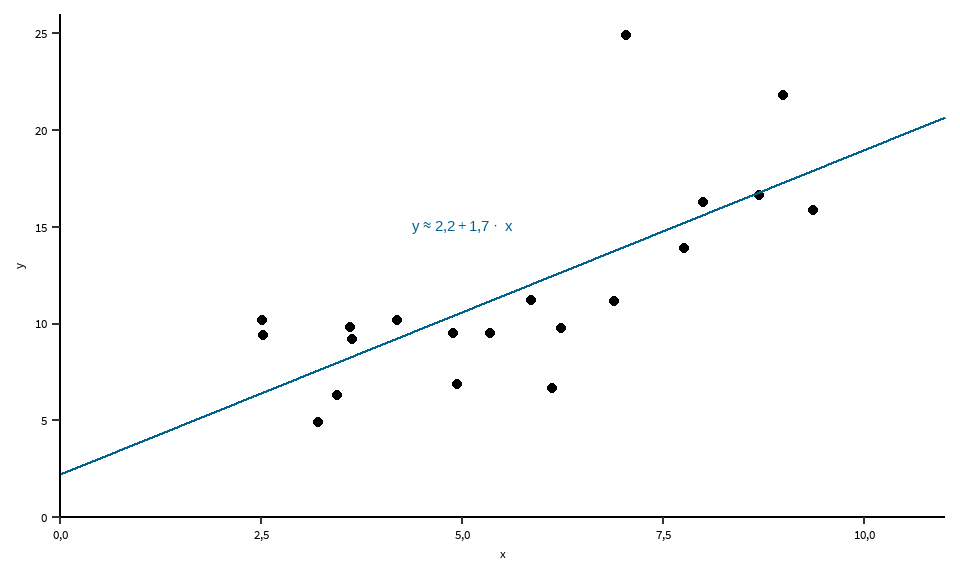
\includegraphics[width=.49\linewidth]{bookdownproj_files/figure-latex/lin-1} 

}

\caption{Regressionslinie durch ein Streudiagramm}\label{fig:lin}
\end{figure}

Der Achsenabschnitt \(a\approx2,2\) bedeutet, dass die Regressionsgerade die \(y\)-Achse etwa auf der Höhe 2,2 schneidet (bei \(x=0\)). Die Steigung \(b\approx1,7\) heißt, dass für jede zusätzliche Einheit der Variable \(x\) ca. 1,7 zusätzliche Einheiten der Variable \(y\) erwartet werden können.

Wenn die Regressionsgleichung bekannt ist, kann für jedes gültige (grundsätzlich: jedes beliebige) \(x\) ein erwarteter Wert \(\hat{y}\) berechnet werden. So könnte uns bei der Beispielregression interessieren, welchen Wert \(\hat{y}_i\) im Modell annimmt, wenn \(x_i=20\) beträgt:

\[\begin{aligned}
\hat{y}_i&=a+b\cdot x_i\\
   &\approx2,2+1,7\cdot20\\
   &=36,2
\end{aligned}\]

Bei solchen Schätzungen \emph{außerhalb} des bekannten Wertebereichs spricht man auch vom ``Extrapolieren'', sonst -- für fehlende Werte innerhalb des bekannten Wertebereich -- vom ``Interpolieren''.

Umgekehrt könnte die Frage lauten: Wie groß muss ein \(x_i\) sein, damit (im Modell) \(\hat{y}_i=12\) beträgt? Dies lässt sich durch eine einfache Umformung der \autoref{eq:lin} berechnen:

\[\begin{aligned}
\hat{y}_i&=a+b\cdot x_i\\[5pt]
x_i&=\frac{\hat{y}_i-a}{b}\\[5pt]
&=\frac{12-2,2}{1,7}\\
   &\approx5,8
\end{aligned}\]

Bei der Regressionsanalyse wird ein gerichtetes Abhängigkeitsverhältnis der Variablen impliziert: \(y\) hängt hier von \(x\) ab. Daher wird \(x\) auch die ``Prädiktorvariable'' und \(y\) die ``Kriteriumsvariable'' genannt.

\begin{rtip}
Wenn in R ein lineares Modell (eine Regressionsgerade) vorliegt, können Werte mit {\tt predict() } geschätzt werden.
\end{rtip}

Es ist also für derartige Fragestellungen nötig, die Gleichung der Regressionsgeraden zu kennen. Im Folgenden wird gezeigt, wie diese anhand einer bivariaten Verteilung bestimmt werden kann.

\hypertarget{bestimmung-der-regressionsgeraden}{%
\subsection{Bestimmung der Regressionsgeraden}\label{bestimmung-der-regressionsgeraden}}

Der Koeffizient \(b\) (also die Steigung der Regressionsgeraden) lässt sich berechnen, indem man die Kovarianz \(s_{xy}\) durch die Varianz von \(x\) dividiert:

\[
b=\frac{s_{xy}}{s^2_x}
\]\{\#eq:b\}

Der Koeffizient \(a\) (also der Achsenabschnitt) ergibt sich wiederum aus \(b\) und den Mittelwerten \(\bar{x}\) und \(\bar{y}\):

\nopagebreak

\[
a=\bar{y}-b\cdot\bar{x}
\]\{\#eq:a\}

\begin{rtip}
In R lässt sich ein lineares Regressionsmodell mit dem Befehl {\tt lm() } erstellen.
\end{rtip}

Die Bestimmung der Regressionsgeraden soll nun mit einem Beispiel illustriert werden.

\hypertarget{beispiel-26}{%
\subsubsection{Beispiel}\label{beispiel-26}}

Wir fragen uns, wie die Aufenthaltszeit von Passagieren am Frankfurter Flughafen mit dem Betrag zusammenhängt, den sie in den dortigen Geschäften ausgeben. Eine Zufallserhebung habe die Werte in \autoref{tab:duty} ergeben.

\begin{table}

\caption{\label{tab:unnamed-chunk-24}\label{tab:duty}Messwerte am Frankfurter Flughafen}
\centering
\begin{tabular}[t]{rr}
\toprule
\multicolumn{1}{c}{Aufenthaltszeit (min)} & \multicolumn{1}{c}{Ausgaben (€)} \\
\cmidrule(l{3pt}r{3pt}){1-1} \cmidrule(l{3pt}r{3pt}){2-2}
$x_i$ & $y_i$\\
\midrule
121 & 17,94\\
125 & 23,15\\
293 & 44,31\\
370 & 42,46\\
246 & 35,51\\
281 & 28,46\\
169 & 18,47\\
328 & 56,77\\
388 & 40,11\\
131 & 12,64\\
299 & 24,54\\
324 & 46,37\\
\bottomrule
\end{tabular}
\end{table}

Mit den Methoden aus Sitzung 2 und 7 können wir folgende Werte für die Mittelwerte \(\bar{x}\) und \(\bar{y}\), die Varianz \(s^2_x\) sowie die Kovarianz \(s_{xy}\) berechnen:

\[\begin{aligned}
\bar{x}&=256,25\\
\bar{y}&\approx 32,56\\
s^2_{x}&\approx9340,93\\
s_{xy}&\approx 1062,50
\end{aligned}\]

Für die Steigung der Regressionsgeraden \(b\) setzen wir die entsprechenden Werte in \autoref{eq:b} ein:

\nopagebreak

\[\begin{aligned}
b&=\frac{s_{xy}}{s^2_x}\\[5pt]
 &\approx\frac{1062,50}{9340,93}\\[4pt]
 &\approx0,114
\end{aligned}\]

Die Steigung von 0,114 bedeutet, dass -- im linearen Regressionsmodell -- Passagiere in jeder zusätzlichen Minute, die sie am Flughafen verbringen, in etwa 11,4 zusätzliche Cent ausgeben.

Der Achsenabschnitt \(a\) berechnet sich dann gemäß \autoref{eq:a}:

\nopagebreak

\[\begin{aligned}
a&=\bar{y}-b\cdot\bar{x}\\
&\approx 32,56-0,114\cdot256,25\\
&\approx 3,35
\end{aligned}\]

Dieser Wert ergibt nur einen abstrakt-mathematischen Sinn -- es dürfte in der Praxis wohl kaum Passagiere geben, die 0 Minuten am Flughafen verbringen und € 3,35 ausgeben.

Mit dem Achsenabschnitt \(a\) und der Steigung \(b\) lässt sich folgende Gleichung für die Regressionsgerade aufstellen (s. \autoref{eq:lin}):

\[\begin{aligned}
y&=a+b\cdot x\\
y&\approx3,35 + 0,114 \cdot x
\end{aligned}\]

Graphisch ist diese lineare Regression in \autoref{fig:duty} dargestellt.

\begin{figure}[h]

{\centering 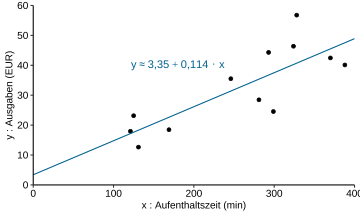
\includegraphics[width=.49\linewidth]{bookdownproj_files/figure-latex/duty-1} 

}

\caption{Regressionslinie durch ein Streudiagramm}\label{fig:duty}
\end{figure}

\hypertarget{residuen}{%
\subsection{Residuen}\label{residuen}}

Residuen (engl. \emph{residuals}) werden mit \(e\) bezeichnet und sind die Differenzen zwischen den tatsächlichen \(y\)-Werten und den im Modell erwarteten \(\hat{y}\)-Werten für die jeweiligen \(x\)-Werte:

\nopagebreak

\[
e_i=y_i-\hat{y}_i
\]\{\#eq:res\}

Residuen sind also -- auch dem Wortstamm nach -- das, was nach der Vorhersage durch das Modell ``übrig bleibt'' von den tatsächlich beobachteten Werten (also der Teil des Werts, der \emph{nicht} durch das Regressionsmodell erklärt wird).

\begin{rtip}
Residuen lassen sich in R durch den Befehl {\tt resid() } errechnen.
\end{rtip}

\hypertarget{beispiel-27}{%
\subsubsection{Beispiel}\label{beispiel-27}}

Graphisch sind die Residuen für unser Beispiel in \autoref{fig:res} dargestellt (positive Werte in grün, negative Werte in rot), tabellarisch in \autoref{tab:res}.

\begin{figure}[h]

{\centering 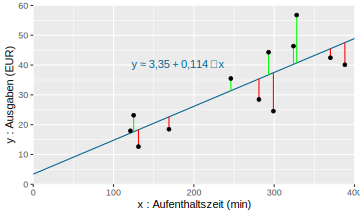
\includegraphics[width=.49\linewidth]{bookdownproj_files/figure-latex/res-1} 

}

\caption{Graphische Darstellung der Residuen}\label{fig:res}
\end{figure}

\begin{table}

\caption{\label{tab:unnamed-chunk-25}\label{tab:res}Residuen der Beispielwerte}
\centering
\begin{tabular}[t]{rrrr}
\toprule
\multicolumn{1}{c}{Aufenthaltszeit (min)} & \multicolumn{1}{c}{Ausgaben (€)} & \multicolumn{1}{c}{Erwartete Ausgaben (€)} & \multicolumn{1}{c}{Residuen (€)} \\
\cmidrule(l{3pt}r{3pt}){1-1} \cmidrule(l{3pt}r{3pt}){2-2} \cmidrule(l{3pt}r{3pt}){3-3} \cmidrule(l{3pt}r{3pt}){4-4}
$x_i$ & $y_i$ & $\hat{y}_i\approx3,35+0,114\cdot x_i$ & $e_i=y_i-\hat{y}_i$\\
\midrule
121 & 17,94 & 17,144 & 0,796\\
125 & 23,15 & 17,600 & 5,550\\
293 & 44,31 & 36,752 & 7,558\\
370 & 42,46 & 45,530 & -3,070\\
246 & 35,51 & 31,394 & 4,116\\
281 & 28,46 & 35,384 & -6,924\\
169 & 18,47 & 22,616 & -4,146\\
328 & 56,77 & 40,742 & 16,028\\
388 & 40,11 & 47,582 & -7,472\\
131 & 12,64 & 18,284 & -5,644\\
299 & 24,54 & 37,436 & -12,896\\
324 & 46,37 & 40,286 & 6,084\\
\bottomrule
\end{tabular}
\end{table}

Residuen spielen in vielen statistischen Verfahren eine Rolle, z.B. in der Residuenanalyse. Diese Verfahren werden im Rahmen dieser Veranstaltung jedoch nicht behandelt.

\hypertarget{determinationskoeffizient}{%
\subsection{Determinationskoeffizient}\label{determinationskoeffizient}}

Der Determinationskoeffizient \(R^2\) (engl. \emph{coefficient of determination}) ist formal definiert als das Verhältnis der Varianz der vorhergesagten \(\hat{y}\)-Werte zur Varianz der tatsächlich beobachteten \(y\)-Werte (wobei sich der Term \([n-1]\) auskürzt):

\[
R^2=\frac{\sum\limits^n_{i=1}(\hat{y}_i-\bar{y})^2}{\sum\limits^n_{i=1}(y_i-\bar{y})^2}
\]\{\#eq:rsqformal\}

Da Zähler und Nenner als Quadratsummen stets positiv sind und die Varianz der \(\hat{y}\)-Werte immer \emph{kleiner oder gleich} der Varianz der \(y\)-Werte ist, nimmt der Determinationskoeffizient immer einen Wert zwischen 0 und 1 an.

Je größer \(R^2\), desto besser erklärt das lineare Regressionsmodell die tatsächlich beobachteten Werte. \(R^2=1\) bedeutet, dass das Modell die Werte perfekt erklärt.

Für lineare Regressionsmodelle (also für die einzige Regression, die im Rahmen dieser Veranstaltung behandelt wird) lässt sich \(R^2\) auch berechnen, indem wir den Korrelationskoeffizienten \(r\) quadrieren:

\[
R^2=r^2
\]\{\#eq:rsq\}

\begin{rtip}
In R wird mit dem Befehl {\tt summary()} unter anderem der Determinationskoeffizient eines linearen Regressionsmodells ausgegeben.
\end{rtip}

\hypertarget{beispiel-28}{%
\subsubsection{Beispiel}\label{beispiel-28}}

Mit den Methoden aus Sitzung 7 können wir den Korrelationskoeffizienten für unser Beispiel errechnen:

\[\begin{aligned}
r&=\frac{s_{xy}}{s_x\cdot s_y}\\[6pt]
&\approx\frac{1062,50}{96,65\cdot13,68}\\[4pt]
&\approx0,804
\end{aligned}\]

Der Determinationskoeffizient ergibt sich dann mit \autoref{eq:rsq}:

\[\begin{aligned}
R^2&=r^2\\
&\approx 0,804^2\\
&\approx 0,646
\end{aligned}\]

\hypertarget{aufgaben-7}{%
\subsection{Aufgaben}\label{aufgaben-7}}

\hypertarget{aufgabe-1-7}{%
\subsubsection{Aufgabe 1}\label{aufgabe-1-7}}

Sie haben für eine bivariate Verteilung die folgende Regressionsgleichung bestimmt:

\[
y=-1,48-0,975\cdot x
\]

\begin{enumerate}
\def\labelenumi{\alph{enumi})}
\tightlist
\item
  Bestimmen Sie die erwarteten \(\hat{y}_i\)-Werte für diese \(x_i\)-Werte:
\end{enumerate}

\[
0,3\quad-18,5\quad-13,5\quad-17,2\quad29,8\quad25,6\quad-36,4\quad-26,2
\]

\begin{enumerate}
\def\labelenumi{\alph{enumi})}
\setcounter{enumi}{1}
\tightlist
\item
  Für welche Werte \(x_i\) sagt das Regressionsmodell diese Werte \(\hat{y}_i\) voraus?
\end{enumerate}

\[
-10\quad15\quad-50\quad-10\quad-60\quad-55\quad-20\quad0
\]

\begin{enumerate}
\def\labelenumi{\alph{enumi})}
\setcounter{enumi}{2}
\tightlist
\item
  Bestimmen Sie die Residuen für die tatsächlich beobachtete Messreihe:
\end{enumerate}

\begin{table}
\centering
\begin{tabular}{rr}
\toprule
$x_i$ & $y_i$\\
\midrule
-11,49 & 6,82\\
8,22 & -8,59\\
-25,66 & 25,92\\
23,81 & -26,91\\
-3,14 & 4,41\\
-1,52 & -3,39\\
20,15 & -19,89\\
-10,22 & 9,30\\
\bottomrule
\end{tabular}
\end{table}

\hypertarget{aufgabe-2-7}{%
\subsubsection{Aufgabe 2}\label{aufgabe-2-7}}

Eine bivariate Verteilung sei gekennzeichnet durch die folgenden Parameter:

\[\begin{aligned}
\bar{x}&=157,5\\
\bar{y}&=156,7\\
s^2_{x}&=1080,94\\
s^2_{y}&=884,46\\
s_{xy}&=869,83
\end{aligned}\]

\begin{enumerate}
\def\labelenumi{\alph{enumi})}
\item
  Bestimmen Sie die Regressionsgleichung im linearen Modell.
\item
  Bestimmen Sie den Determinationskoeffizienten \(R^2\).
\end{enumerate}

\hypertarget{aufgabe-3-5}{%
\subsubsection{Aufgabe 3}\label{aufgabe-3-5}}

\emph{Diese Aufgabe erfordert auch Verfahren aus Sitzung 6.}

Sie fragen sich, wie die erreichte Punktzahl in einer Klausur mit der Vorbereitungszeit der geprüften Studierenden zusammenhängt. Sie erheben die folgende Messreihe:

\begin{table}
\centering
\begin{tabular}{rr}
\toprule
Vorbereitungszeit (min) & Erreichte Punktzahl\\
\midrule
834 & 88\\
17 & 41\\
519 & 75\\
253 & 39\\
739 & 77\\
844 & 100\\
\bottomrule
\end{tabular}
\end{table}

\begin{enumerate}
\def\labelenumi{\alph{enumi})}
\item
  Welche Punktzahl ist mit einer Vorbereitunszeit von sechs Stunden zu erwarten?
\item
  Ab welcher Vorbereitungszeit ist im Modell zu erwarten, dass ein Studierende*r die Klausur besteht (\(\geq\) 50 Punkte)?
\item
  Ab welcher Vorbereitungszeit kann laut Modell mit der vollen Punktzahl (100 Punkte) gerechnet werden?
\item
  Wie gut erklärt ein lineares Modell die Prüfungsleistungen anhand der Vorbereitungszeit?
\item
  Welche Limitationen hat das Modell? Denken Sie an extreme Werte.
\end{enumerate}

\hypertarget{tipps-zur-vertiefung-7}{%
\subsection{Tipps zur Vertiefung}\label{tipps-zur-vertiefung-7}}

\begin{itemize}
\tightlist
\item
  Kapitel 11 in \protect\hyperlink{ref-bortz}{Bortz und Schuster} (\protect\hyperlink{ref-bortz}{2010})
\item
  Kapitel 6.2 in \protect\hyperlink{ref-bahrenberg}{Bahrenberg, Giese und Nipper} (\protect\hyperlink{ref-bahrenberg}{2010})
\item
  Kapitel 17 in \protect\hyperlink{ref-klemm}{Klemm} (\protect\hyperlink{ref-klemm}{2002})
\end{itemize}

\hypertarget{quellen-7}{%
\subsection{Quellen}\label{quellen-7}}

\hypertarget{kreuztabellen}{%
\section{Kreuztabellen}\label{kreuztabellen}}

\hypertarget{lernziele-dieser-sitzung-8}{%
\subsection{Lernziele dieser Sitzung}\label{lernziele-dieser-sitzung-8}}

Sie können\ldots{}

\begin{itemize}
\tightlist
\item
  eine Kreuztabelle erstellen und interpretieren.
\item
  den Kontingenzkoeffizienten \(\chi^2\) errechnen.
\item
  die Maßzahlen \(\phi\) bzw. \(\mathit{CI}\) errechnen und interpretieren.
\end{itemize}

\hypertarget{bivariate-verteilungen-mit-nominalen-variablen}{%
\subsection{Bivariate Verteilungen mit nominalen Variablen}\label{bivariate-verteilungen-mit-nominalen-variablen}}

In der bivariaten Statistik (Sitzungen 7 und 8) ging es bisher um Zusammenhänge zwischen zwei metrischen Variablen. In dieser Sitzung geht es um statistische Verfahren der bivariaten Statistik, bei denen für beide Variablen nur das Nominalskalenniveau vorausgesetzt ist. (Für Skalenniveaus s. Sitzung~1.)

Mit den Werten von nominalen Variablen lassen sich die in Sitzung 7 und 8 besprochenen Parameter (z.B. Kovarianz) nicht errechnen, weil wir mit ihnen nicht die notwendigen Rechenoperationen (Addition, Subtraktion) durchführen können. Stattdessen sind die beobachteten Häufigkeiten Ausgangslage für die im Folgenden besprochenen Verfahren.

\hypertarget{beispiel-29}{%
\subsubsection{Beispiel}\label{beispiel-29}}

Wir fragen uns, ob es einen Zusammenhang zwischen dem Studienfach von Studierenden an einer Universität und ihrem präferierten Transportmittel für den Pendelweg zum Campus gibt. Insbesondere interessiert uns, ob ein Zusammenhang zwischen dem Studium der Geistes- und Sozialwissenschaften und der Fahrradnutzung besteht.

Beide Variablen sind nominalskaliert: die erhobenen Werte können in Kategorien eingeordnet werden (Studienfach: Geographie, Politikwissenschaft, BWL, \ldots; Transportmittel: Bus, Fahrrad, zu Fuß, \ldots).

Um die Variablen im Sinne unserer Fragestellung zu vereinfachen, wandeln wir beide Variablen in \emph{dichotome} Variablen um (die dann nur zwei Werte annehmen können). Wir beschränken uns auf die Erhebung von ``Fahrrad'' oder ``anderes Transportmittel'' einerseits und ``Geistes-/Sozialwissenschaft'' oder ``anderes Studienfach'' andererseits. Die (verkürzte) Tabelle der Rohdaten einer Zufallsstichprobe der Größe \(n=90\) könnte dann so aussehen wie \autoref{tab:roh}.

\begin{table}

\caption{\label{tab:unnamed-chunk-28}\label{tab:roh}Ungeordnete Rohdaten der Erhebung}
\centering
\begin{tabular}[t]{lll}
\toprule
  & Studienfach & Transportmittel\\
\midrule
\cellcolor{gray!6}{1} & \cellcolor{gray!6}{anderes Studienfach} & \cellcolor{gray!6}{Fahrrad}\\
2 & anderes Studienfach & Fahrrad\\
\cellcolor{gray!6}{3} & \cellcolor{gray!6}{Geistes-/Sozialwissenschaft} & \cellcolor{gray!6}{anderes Transportmittel}\\
4 & Geistes-/Sozialwissenschaft & anderes Transportmittel\\
\cellcolor{gray!6}{5} & \cellcolor{gray!6}{Geistes-/Sozialwissenschaft} & \cellcolor{gray!6}{anderes Transportmittel}\\
6 & Geistes-/Sozialwissenschaft & Fahrrad\\
\cellcolor{gray!6}{...} & \cellcolor{gray!6}{...} & \cellcolor{gray!6}{...}\\
85 & anderes Studienfach & anderes Transportmittel\\
\cellcolor{gray!6}{86} & \cellcolor{gray!6}{anderes Studienfach} & \cellcolor{gray!6}{anderes Transportmittel}\\
87 & Geistes-/Sozialwissenschaft & anderes Transportmittel\\
\cellcolor{gray!6}{88} & \cellcolor{gray!6}{anderes Studienfach} & \cellcolor{gray!6}{anderes Transportmittel}\\
89 & anderes Studienfach & anderes Transportmittel\\
\cellcolor{gray!6}{90} & \cellcolor{gray!6}{Geistes-/Sozialwissenschaft} & \cellcolor{gray!6}{anderes Transportmittel}\\
\bottomrule
\end{tabular}
\end{table}

\hypertarget{kreuztabelle}{%
\subsection{Kreuztabelle}\label{kreuztabelle}}

Die Kreuztabelle (auch Kontingenztabelle, Kontingenztafel, engl. \emph{contingency table}) ist eine übersichtliche Zusammenfassung der Rohdaten. Sie spannt die beiden Variablen in Spalten- und Zeilenrichtung auf, so dass in jeder Zelle die Häufigkeit einer bestimmten Wertekombination steht.

Bei zwei dichotomen Variablen ergeben sich zwei Spalten und zwei Zeilen, also vier Tabellenfelder. Wir sprechen in diesem Fall auch von einer \(2\times2\)-Tabelle.

\hypertarget{beispiel-30}{%
\subsubsection{Beispiel}\label{beispiel-30}}

Die Kreuztabelle für unser Beispiel ist in \autoref{tab:crossrad} dargestellt. Die Spaltenüberschriften sind die beiden Werte der dichotomen Variable ``Transportmittel'', und die Zeilennamen sind die beiden Werte für ``Studienfach''. In den Zellen stehen die Häufigkeiten. Es lässt sich also z.B. ablesen, dass die Kombination ``Fahrrad'' und ``anderes Studienfach'' neun mal vorkommt.

\begin{table}

\caption{\label{tab:crossrad}Kreuztabelle der Beispieldaten}
\centering
\begin{tabular}[t]{>{}r|r>{}r|r}
\toprule
 & Fahrrad & anderes Transportmittel & \\
\midrule
Geistes-/Sozialwissenschaft & \makecell[tr]{11} & \makecell[tr]{28} & 39\\
anderes Studienfach & \makecell[tr]{9} & \makecell[tr]{42} & 51\\
\midrule
 & 20 & 70 & 90\\
\bottomrule
\end{tabular}
\end{table}

Am rechten Rand der Tabelle stehen die Summen für die Zeilen, am unteren Rand die Summen der Spalten. Ganz unten rechts steht die Gesamtsumme (Größe der Stichprobe).

\begin{rtip}
In R kann eine einfache Kreuztabelle mit dem Befehl {\tt table()} ausgegeben werden.
\end{rtip}

\hypertarget{verallgemeinerung}{%
\subsubsection{Verallgemeinerung}\label{verallgemeinerung}}

In \autoref{tab:crossalg} ist das allgemeingültige Format für Kreuztabellen festgehalten. Dabei sind folgende Besonderheiten zu beachten:

\begin{itemize}
\tightlist
\item
  Das Symbol \(k\) steht für die Anzahl der Zeilen, \(\ell\) für die Anzahl der Spalten.
\item
  Die Häufigkeiten für Merkmalskombinationen in den Tabellenfeldern werden durch \(n_{ij}\) symbolisiert, wobei \(i\) für die laufende Nummer der Zeile steht, und \(j\) für die laufende Nummer der Spalte.
\item
  Die Teilsummen an den Rändern werden mit Punktnotation bezeichnet. Dabei steht die Zeilensumme \(n_{i\cdot}\) für die Summe \emph{aller} Felder in Zeile \(i\) (Zeilensumme) und \(n_{\cdot j}\) für die Summe \emph{aller} Felder in Spalte \(j\) (Spaltensumme).
\item
  Die Gesamtsumme unten rechts wird hier mit \(n\) gekennzeichnet und steht wie gewohnt für die Gesamtgröße der Stichprobe.
\end{itemize}

\begin{table}

\caption{\label{tab:crossalg}Allgemeine Bezeichnungen in der Kreuztabelle}
\centering
\begin{tabular}[t]{>{}l|lll>{}l|l}
\toprule
  & Spalte 1 & Spalte 2 & ... & Spalte $\ell$ & \\
\midrule
Zeile 1 & $n_{11}$ & $n_{12}$ & ... & $n_{1\ell}$ & $n_{1\cdot}$\\
Zeile 2 & $n_{21}$ & $n_{22}$ & ... & $n_{2\ell}$ & $n_{2\cdot}$\\
... & ... & ... & ... & ... & ...\\
Zeile $k$ & $n_{k1}$ & $n_{k2}$ & ... & $n_{k\ell}$ & $n_{k\cdot}$\\
\midrule
 & $n_{\cdot1}$ & $n_{\cdot2}$ & ... & $n_{\cdot\ell}$ & $n$\\
\bottomrule
\end{tabular}
\end{table}

\hypertarget{berechnung-der-erwarteten-werte}{%
\subsection{Berechnung der erwarteten Werte}\label{berechnung-der-erwarteten-werte}}

Bestünde \emph{kein} Zusammenhang zwischen den Variablen, dann wäre zu erwarten, dass sich die Kombinationen gleichmäßig auf die Tabellenfelder aufteilen, und zwar ausgehend von den Teilsummen für die Zeilen und Spalten.

Der Erwartungswert für ein Tabellenfeld (also der ``durchschnittliche'' Wert, wenn es keinen Zusammenhang zwischen den beiden Variablen gibt) berechnet sich durch die Formel:

\nopagebreak

\[
m_{ij}=\frac{n_{i\cdot}\cdot n_{\cdot j}}{n}
\]\{\#eq:m\}

Es wird also das Produkt der Zeilen- und der Spaltensumme geteilt durch die Gesamtsumme.

\hypertarget{beispiel-31}{%
\subsubsection{Beispiel}\label{beispiel-31}}

Die beobachtete Häufigkeit für die Kombination ``Geistes-/Sozialwissenschaft'' (Zeile 1) und ``anderes Transportmittel'' (Spalte 2) ist 28. Aber was wäre der Erwartungswert bei den gegebenen Summen? Wir setzen einfach die entsprechenden Werte in die \autoref{eq:m} ein:

\nopagebreak

\[\begin{aligned}
m_{12}&=\frac{n_{1\cdot}\cdot n_{\cdot 2}}{n}\\[5pt]
&=\frac{39\cdot 70}{90}\\[4pt]
&\approx 30,33
\end{aligned}\]

Diese Rechnung lässt sich für alle Tabellenfelder durchführen. Die Kreuztabelle kann dann um diese erwarteten Werte in Klammern ergänzt werden (s. \autoref{tab:expected}).

\begin{table}

\caption{\label{tab:expected}Kreuztabelle der Beispieldaten}
\centering
\begin{tabular}[t]{>{}r|r>{}r|r}
\toprule
 & Fahrrad & anderes Transportmittel & \\
\midrule
Geistes-/Sozialwissenschaft & \makecell[tr]{11\\(8,67)} & \makecell[tr]{28\\(30,33)} & 39\\
anderes Studienfach & \makecell[tr]{9\\(11,33)} & \makecell[tr]{42\\(39,67)} & 51\\
\midrule
 & 20 & 70 & 90\\
\bottomrule
\end{tabular}
\end{table}

\hypertarget{berechnung-des-kontingenzkoeffizenten-chi2}{%
\subsection{\texorpdfstring{Berechnung des Kontingenzkoeffizenten \(\chi^2\)}{Berechnung des Kontingenzkoeffizenten \textbackslash chi\^{}2}}\label{berechnung-des-kontingenzkoeffizenten-chi2}}

Sind für alle Tabellenfelder die Beobachtungs- und Erwartungswerte gegeben, lässt sich für jedes Tabellenfeld ein Wert berechnen, der diese Werte in Relation setzt. Die Summe dieser Werte über die gesamte Tabelle hinweg wird Kontingenzkoeffizient genannt und mit \(\chi^2\) (``Chi-Quadrat'') abgekürzt.

\nopagebreak

\[
\chi^2= \sum_{i=1}^{k}\sum_{j=1}^{\ell}\frac{(n_{ij}-m_{ij})^{2}}{m_{ij}}
\]\{\#eq:chisq\}

Bei der Formel steht \(k\) wieder für die Anzahl der Zeilen (und \(i\) für ihre laufende Nummer) und \(\ell\) für die Anzahl der Spalten (und \(j\) für ihre laufende Nummer).

Das doppelte Summenzeichen mag etwas verwirrend sein, bedeutet aber nur, dass die Zeilen spaltenweise summiert werden, und dann die Summe dieser Zeilensumme genommen wird -- d.h. dass einfach alle Tabellenfelder aufsummiert werden.

Der \(\chi^2\)-Wert kann (ähnlich wie der \(F\)-Wert aus Sitzung 6) nur positive Werte annehmen. Er bildet die Grundlage für die im Folgenden besprochenen Kennwerte \(\phi\) und \(\mathit{CI}\) sowie für den in Sitzung 10 zu besprechenden \(\chi^2\)-Test.

\hypertarget{beispiel-32}{%
\subsubsection{Beispiel}\label{beispiel-32}}

Ein möglicher Zwischenschritt ist es, diese Teilwerte von \(\chi^2\) für die einzelnen Tabellenfelder auszurechnen und in der Kreuztabelle zu notieren. Die Teilwerte werden dann für jedes Tabellenfeld mit der Formel

\nopagebreak

\[
\frac{(n_{ij}-m_{ij})^{2}}{m_{ij}}
\]\{\#eq:contrib\}

berechnet und sind in \autoref{tab:radchisq} in blau dargestellt.

\begin{table}

\caption{\label{tab:radchisq}Kreuztabelle der Beispieldaten mit Teilwerten für $\chi^2$}
\centering
\begin{tabular}[t]{>{}r|r>{}r|r}
\toprule
 & Fahrrad & anderes Transportmittel & \\
\midrule
Geistes-/Sozialwissenschaft & \makecell[tr]{11\\(8,67)\\\textcolor{goethe_blue}{0,626}} & \makecell[tr]{28\\(30,33)\\\textcolor{goethe_blue}{0,179}} & 39\\
anderes Studienfach & \makecell[tr]{9\\(11,33)\\\textcolor{goethe_blue}{0,479}} & \makecell[tr]{42\\(39,67)\\\textcolor{goethe_blue}{0,137}} & 51\\
\midrule
 & 20 & 70 & 90\\
\bottomrule
\end{tabular}
\end{table}

Zum Beispiel ergibt sich der Teilwert für \(\chi^2\) für die Kombination ``anderes Studienfach'' -- ``Fahrrad'' durch Einsetzen in \autoref{eq:contrib}:

\nopagebreak

\[\begin{aligned}
\frac{(n_{21}-m_{21})^{2}}{m_{21}} &\approx \frac{(9-11,33)^2}{11,33}\\
&=\frac{-2,33^2}{11,33}\\
&\approx\frac{5,43}{11,33}\\
&\approx0,479
\end{aligned}\]

Der \(\chi^2\)-Wert lässt sich nun bestimmen, indem diese Teilwerte aufsummiert werden:

\[\begin{aligned}
\chi^2&= \sum_{i=1}^{k}\sum_{j=1}^{\ell}\frac{(n_{ij}-m_{ij})^{2}}{m_{ij}}\\[4pt]
&\approx 0,626 + 0,179 + 0,479 + 0,137\\
& =1,421
\end{aligned}\]

Mit diesem Wert \(\chi^2\approx1,421\) können wir noch nicht so viel anfangen -- wir wissen aber, dass er ein Maß dafür ist, wie sehr unsere beobachtete Verteilung von einer zu erwarteten Verteilung (vorausgesetzt, es gibt keinen Zusammenhang) abweicht.

\hypertarget{berechnung-des-phi-koeffizienten}{%
\subsection{\texorpdfstring{Berechnung des \(\phi\)-Koeffizienten}{Berechnung des \textbackslash phi-Koeffizienten}}\label{berechnung-des-phi-koeffizienten}}

Der \(\phi\)-Koeffizient ist der Korrelationskoeffizient für zwei dichotome Variablen (wobei er in der hier besprochenen Version nur positive Werte annehmen kann). Er ist jedoch \emph{nicht} ohne weiteres mit dem Korrelationskoeffizienten \(r\) (aus Sitzung 7) vergleichbar.

Der Wert für \(\phi\) kann aus \(\chi^2\) berechnet werden mit:

\nopagebreak

\[
\phi=\sqrt{\frac{\chi^2}{n}}
\]\{\#eq:phi\}

\hypertarget{beispiel-33}{%
\subsubsection{Beispiel}\label{beispiel-33}}

In unserem Beispiel ergibt sich also für \(\phi\) durch Einsetzung in \autoref{eq:phi}:

\nopagebreak

\[\begin{aligned}
\phi&=\sqrt{\frac{\chi^2}{n}}\\[6pt]
    &\approx\sqrt{\frac{1,421}{90}}\\[4pt]
    &\approx0,126
\end{aligned}\]

Es wird ersichtlich, dass es eine leichte Korrelation der Variablen gibt. Aber in welche Richtung? Dafür müssen wir auf die Kreuztabelle blicken: Der beobachtete Wert für die Wertekombination ``Fahrrad'' und ``Geistes-/Sozialwissenschaft'' beträgt \(n_{11}=11\) und liegt über dem Erwartungswert \(m_{11}=8,67\). Damit ist klar: Das Studium von Geistes- und Sozialwissenschaften korreliert \emph{positiv} mit der Fahrradnutzung für den Pendelweg.

Ob diese Korrelation auch statistisch relevant ist, kann mit dem \(\chi^2\)-Test (Sitzung 10) überprüft werden.

\hypertarget{berechnung-des-cramuxe9r-index}{%
\subsection{Berechnung des Cramér-Index}\label{berechnung-des-cramuxe9r-index}}

Bisher wurden in dieser Sitzung nur Verteilungen von zwei dichotomen Variablen besprochen. Nun gibt es aber auch nominalskalierte bivariate Verteilungen, in denen die Merkmale mehr als zwei Werte annehmen können (also nicht dichotom sind). In diesem Fall ist der Cramér-Index (auch Cramérs \(v\), engl. \emph{Cramér index}) ein geeigneter Kennwert für die Abhängigkeit der Variablen.

Die Formel für den Cramér-Index lautet

\[
\mathit{CI}=\sqrt{\frac{\chi^2}{n\cdot (\mathrm{min}(k, \ell)-1)}}
\]\{\#eq:ci\}

wobei der Ausdruck \(\mathrm{min}(k,\ell)\) für den \emph{kleineren} Wert aus Zeilenanzahl \(k\) und Spaltenanzahl \(\ell\) steht.

In einer \(2\times2\)-Tabelle ist dieser Wert identisch mit dem \(\phi\)-Koeffizienten.

\hypertarget{beispiel-34}{%
\subsubsection{Beispiel}\label{beispiel-34}}

Hätten wir im Beispiel die Erhebung nicht auf dichotome Variablen reduziert, sondern die Wissenschaftsdisziplinen und Verkehrsmittel direkt erhoben, so würde sich die Kreuztabelle vielleicht wie in \autoref{tab:ci} darstellen.

Dabei werden die Erwartungswerte wie gehabt mit \autoref{eq:m} und die Teilwerte für \(\chi^2\) mit der \autoref{eq:contrib} errechnet.

\begin{table}
\centering
\begin{tabular}{>{}r|rr>{}r|r}
\toprule
\multicolumn{1}{c}{ } & \multicolumn{2}{c}{Transportmittel} & \multicolumn{1}{c}{ } \\
Studienfach~$\downarrow$ & Fahrrad & Auto & Öffentliche & \\
\midrule
Geisteswissenschaft & \makecell[tr]{5\\(4,22)\\\textcolor{goethe_blue}{0,144}} & \makecell[tr]{5\\(8,02)\\\textcolor{goethe_blue}{1,137}} & \makecell[tr]{9\\(6,76)\\\textcolor{goethe_blue}{0,742}} & 19\\
Sozialwissenschaft & \makecell[tr]{6\\(4,44)\\\textcolor{goethe_blue}{0,548}} & \makecell[tr]{6\\(8,44)\\\textcolor{goethe_blue}{0,705}} & \makecell[tr]{8\\(7,11)\\\textcolor{goethe_blue}{0,111}} & 20\\
Naturwissenschaft & \makecell[tr]{5\\(5,11)\\\textcolor{goethe_blue}{0,002}} & \makecell[tr]{9\\(9,71)\\\textcolor{goethe_blue}{0,052}} & \makecell[tr]{9\\(8,18)\\\textcolor{goethe_blue}{0,082}} & 23\\
Ingenieurswissenschaft & \makecell[tr]{4\\(6,22)\\\textcolor{goethe_blue}{0,792}} & \makecell[tr]{18\\(11,82)\\\textcolor{goethe_blue}{3,231}} & \makecell[tr]{6\\(9,96)\\\textcolor{goethe_blue}{1,574}} & 28\\
\midrule
 & 20 & 38 & 32 & 90\\
\bottomrule
\end{tabular}
\end{table}

Der \(\chi^2\)-Wert ergibt sich wieder aus der Summe (s. \autoref{eq:chisq}):

\nopagebreak

\[\begin{aligned}
\chi^2&= \sum_{i=1}^{k}\sum_{j=1}^{\ell}\frac{(n_{ij}-m_{ij})^{2}}{m_{ij}}\\[4pt]
&\approx 0,144+1,137+0,742+0,548+0,705+0,111\\&\quad+0,002+0,052+0,082+0,792+3,231+1,574 \\
& =9,120
\end{aligned}\]

Mit diesem Wert kann der Cramér-Index anhand von \autoref{eq:ci} berechnet werden.

Die Zeilenanzahl ist \(k=4\) und die Spaltenanzahl \(\ell=3\). Der Ausdruck \(\mathrm{min}(k,\ell)\) ergibt den kleineren dieser Werte, also 3:

\[\begin{aligned}
\mathit{CI}&=\sqrt{\frac{\chi^2}{n\cdot (\mathrm{min}(k, \ell)-1)}}\\[6pt]
&\approx\sqrt{\frac{9,122}{90\cdot(3-1)}}\\[4pt]
&\approx0,225
\end{aligned}\]

Dieser Wert ist größer als der oben berechnete \(\phi\)-Koeffizient. Das ist nicht besonders überraschend: Eine detailliertere Erfassung der Variablen führt zu einem deutlicheren Zusammenhang.

\hypertarget{aufgaben-8}{%
\subsection{Aufgaben}\label{aufgaben-8}}

\hypertarget{aufgabe-1-8}{%
\subsubsection{Aufgabe 1}\label{aufgabe-1-8}}

Sie fragen sich, wie die Wohnumgebung einer Person (Stadt oder Land) damit zusammenhängt, ob die Person ein eigenes Auto besitzt. Sie erheben die folgende Messreihe:

\begin{table}[!h]
\centering
\begin{tabular}{ll}
\toprule
Wohnort & Autobesitz\\
\midrule
\cellcolor{gray!6}{Land} & \cellcolor{gray!6}{\vphantom{8} Ja}\\
Land & \vphantom{7} Ja\\
\cellcolor{gray!6}{Stadt} & \cellcolor{gray!6}{\vphantom{6} Nein}\\
Stadt & \vphantom{5} Nein\\
\cellcolor{gray!6}{Stadt} & \cellcolor{gray!6}{\vphantom{1} Ja}\\
\addlinespace
Stadt & \vphantom{4} Nein\\
\cellcolor{gray!6}{Land} & \cellcolor{gray!6}{\vphantom{6} Ja}\\
Land & \vphantom{1} Nein\\
\cellcolor{gray!6}{Land} & \cellcolor{gray!6}{\vphantom{5} Ja}\\
Land & \vphantom{4} Ja\\
\addlinespace
\cellcolor{gray!6}{Stadt} & \cellcolor{gray!6}{\vphantom{3} Nein}\\
Land & \vphantom{3} Ja\\
\cellcolor{gray!6}{Land} & \cellcolor{gray!6}{\vphantom{2} Ja}\\
Land & \vphantom{1} Ja\\
\cellcolor{gray!6}{Stadt} & \cellcolor{gray!6}{\vphantom{2} Nein}\\
\addlinespace
Land & Ja\\
\cellcolor{gray!6}{Stadt} & \cellcolor{gray!6}{\vphantom{1} Nein}\\
Land & Nein\\
\cellcolor{gray!6}{Stadt} & \cellcolor{gray!6}{Ja}\\
Stadt & Nein\\
\bottomrule
\end{tabular}
\end{table}

\begin{enumerate}
\def\labelenumi{\alph{enumi})}
\item
  Überführen Sie die Daten in eine Kreuztabelle.
\item
  Berechnen Sie die Erwartungswerte für jedes Tabellenfeld.
\item
  Berechnen Sie \(\chi^2\).
\item
  Berechnen Sie den \(\phi\)-Koeffizienten.
\item
  Besteht eine Korrelation? In welche Richtung?
\end{enumerate}

\hypertarget{aufgabe-2-8}{%
\subsubsection{Aufgabe 2}\label{aufgabe-2-8}}

Sie interessieren sich dafür, ob zwei ``Ja/Nein''-Fragen auf einem Fragebogen korrelieren.

Sie ermittlen folgende Häufigkeiten:

\begin{table}[!h]
\centering
\begin{tabular}{>{}r|rrr}
\toprule
\multicolumn{1}{c}{ } & \multicolumn{2}{c}{Frage 2} \\
Frage 1~$\downarrow$ & Ja & Nein & NA\\
\midrule
Ja & \makecell[tr]{5} & \makecell[tr]{28} & NA\\
Nein & \makecell[tr]{40} & \makecell[tr]{72} & NA\\
\bottomrule
\end{tabular}
\end{table}

\begin{enumerate}
\def\labelenumi{\alph{enumi})}
\item
  Vervollständigen Sie die Kreuztabelle um ihre Summen und die Erwartungswerte.
\item
  Berechnen Sie \(\chi^2\) und den \(\phi\)-Koeffizienten.
\item
  Wie würden Sie den Zusammenhang beschreiben?
\end{enumerate}

\hypertarget{aufgabe-3-6}{%
\subsubsection{Aufgabe 3}\label{aufgabe-3-6}}

Sie möchten überprüfen, ob auf dem Arbeitsmarkt anhand von Namen diskriminiert wird, die auf einen Migrationshintergrund schließen lassen. Sie antworten als fiktive Bewerber*innen mit vergleichbaren Qualifikationen auf zufällige Stellenanzeigen und halten fest, ob die jeweilige Bewerbung in einer Einladung zum Vorstellungsgespräch resultiert.

Sie erheben diese Daten:

\begin{table}
\centering
\begin{tabular}{>{}r|rrr}
\toprule
\multicolumn{1}{c}{ } & \multicolumn{2}{c}{Ergebnis} \\
Herkunft des Namens~$\downarrow$ & eingeladen & nicht eingeladen & NA\\
\midrule
deutsch & \makecell[tr]{36} & \makecell[tr]{64} & NA\\
italienisch & \makecell[tr]{23} & \makecell[tr]{77} & NA\\
slawisch & \makecell[tr]{9} & \makecell[tr]{91} & NA\\
türkisch & \makecell[tr]{11} & \makecell[tr]{89} & NA\\
\bottomrule
\end{tabular}
\end{table}

Können Sie einen Zusammenhang zwischen Namensherkunft und Erfolg der Bewerbung feststellen? Begründen Sie Ihre Antwort.

\hypertarget{tipps-zur-vertiefung-8}{%
\subsection{Tipps zur Vertiefung}\label{tipps-zur-vertiefung-8}}

\begin{itemize}
\tightlist
\item
  Kapitel 9.1, 10.3.4 und 10.3.7 in \protect\hyperlink{ref-bortz}{Bortz und Schuster} (\protect\hyperlink{ref-bortz}{2010})
\item
  Kapitel 6.7.2 in \protect\hyperlink{ref-bahrenberg}{Bahrenberg, Giese und Nipper} (\protect\hyperlink{ref-bahrenberg}{2010})
\item
  Kapitel 2.3 in \protect\hyperlink{ref-klemm}{Klemm} (\protect\hyperlink{ref-klemm}{2002})
\end{itemize}

\hypertarget{quellen-8}{%
\subsection{Quellen}\label{quellen-8}}

\hypertarget{chi-quadrat-tests}{%
\section{Chi-Quadrat-Tests}\label{chi-quadrat-tests}}

\hypertarget{lernziele-dieser-sitzung-9}{%
\subsection{Lernziele dieser Sitzung}\label{lernziele-dieser-sitzung-9}}

Sie können\ldots{}

\begin{itemize}
\tightlist
\item
  einen \(\chi^2\)-Unabhängigkeitstest durchführen.
\item
  einen \(\chi^2\)-Anpassungstest durchführen.
\end{itemize}

\hypertarget{anwendungsbereich}{%
\subsection{Anwendungsbereich}\label{anwendungsbereich}}

In Sitzung 9 haben wir gelernt, wie für bivariate Verteilungen Korrelationen beschrieben werden können, wenn beide Variablen nominalskaliert sind. Grundlage dafür waren die Häufigkeiten von Wertekombinationen in der Kreuztabelle.

Auch für \(\chi^2\)-Tests sind beobachtete Häufigkeiten in einer Kreuztabelle unser Ausgangspunkt. Wir fragen jedoch nicht nach einem Kennwert für die Stärke der Korrelation, sondern wollen wissen, ob es einen statistisch signifikanten Zusammenhang zwischen den beiden Variablen gibt -- also einen Zusammenhang, der nur mit einer Wahrscheinlichkeit \(\alpha\) zufällig zustande gekommen ist.

Um den Unterschied zu verdeutlichen: Bei sehr großen Fallzahlen kann auch eine leichte Korrelation statistisch signifikant sein, bei kleinen Fallzahlen wird es es selbst für starke Korrelationen schwierig, eine statistische Signifikanz nachzuweisen.

Mit dem \(\chi^2\)-Unabhängigkeitstest und dem \(\chi^2\)-Anpassungstest lernen wir im Folgenden zwei leicht unterschiedliche Varianten des \(\chi^2\)-Tests kennen. Beide sollen direkt an Beispielen ausgeführt werden.

\hypertarget{chi2-unabhuxe4ngigkeitstest}{%
\subsection{\texorpdfstring{\(\chi^2\)-Unabhängigkeitstest}{\textbackslash chi\^{}2-Unabhängigkeitstest}}\label{chi2-unabhuxe4ngigkeitstest}}

Grundlage sind bivariate Häufigkeiten, die in einer Kreuztabelle dargestellt werden können (s. \autoref{tab:zivi1}). Wie Kreuztabellen erstellt werden, haben wir bereits in Sitzung 9 behandelt.

\begin{table}

\caption{\label{tab:zivi1}Kreuztabelle der Beispieldaten}
\centering
\begin{tabular}[t]{>{}r|r>{}r|r}
\toprule
 & Grundwehrdienst & Zivildienst & \\
\midrule
Land & \makecell[tr]{18} & \makecell[tr]{11} & 29\\
Stadt & \makecell[tr]{10} & \makecell[tr]{23} & 33\\
\midrule
 & 28 & 34 & 62\\
\bottomrule
\end{tabular}
\end{table}

Unser Beispieldatensatz beschäftigt sich mit Kriegsdienstverweigerern. Zwischen 1956 und 2011 galt in der BRD die Wehrpflicht, d.h. alle vom Staat als ``männlich'' erfassten und als ``tauglich'' gemusterte jungen Menschen mussten Dienst an der Waffe leisten -- es sei denn, sie verweigerten den Kriegsdienst und leisteten stattdessen Zivildienst (z.B. in sozialen Einrichtungen).

Zusätzlich zur Frage der Kriegsdienstverweigerung sei in einer Zufallsstichprobe von als tauglich gemusterten erhoben, ob der Wohnort eine Gemeinde mit über oder unter 20000 Einwohner*innen (``Stadt'' oder ``Land'') ist.\footnote{Hier wird also eine verhältnisskalierte Variable (Bevölkerungszahl der Gemeinde) in eine nominalskalierte Variable transformiert. In Fällen wie diesen, wo die Variable nach der Transformation nur zwei Werte annehmen kann, sprechen wir auch von der ``Dichotomisierung'' einer Variable.} Die Ergebnisse sind in \autoref{tab:zivi1} zusammengefasst.

Wir interessieren uns für den statistischen Zusammenhang dieser beiden Variablen, und zwar möchten wir die Hypothese prüfen, dass Menschen aus der Stadt eher den Kriegsdienst verweigerten als Menschen vom Land. Der Test wird entlang der bekannten sechs Schritte ausgeführt.

\hypertarget{test-wuxe4hlen-und-voraussetzungen-pruxfcfen-4}{%
\subsubsection{Test wählen und Voraussetzungen prüfen}\label{test-wuxe4hlen-und-voraussetzungen-pruxfcfen-4}}

Für den \(\chi^2\)-Unabhängigkeitstest müssen folgende Voraussetzungen erfüllt sein:

\begin{itemize}
\tightlist
\item
  Ziel ist die Überprüfung einer bivariaten Verteilung auf einen statistisch signifikanten Zusammenhang zwischen zwei nominalskalierten Variablen.
\item
  Grundlage sind beobachtete Häufigkeiten aus einer einfachen, unabhängigen Zufallsstichprobe.
\item
  Alle Tabellenfelder enthalten beobachtete Häufigkeiten \((n_{ij}\geq 5)\).
\end{itemize}

Für unsere Beispieldaten sind diese Voraussetzungen gegeben.

\hypertarget{hypothesen-formulieren-4}{%
\subsubsection{Hypothesen formulieren}\label{hypothesen-formulieren-4}}

Wir haben wieder zwei Möglichkeiten: die gerichtete und die ungerichtete Alternativhypothese.

\hypertarget{ungerichtete-alternativhyptothese}{%
\paragraph{Ungerichtete Alternativhyptothese}\label{ungerichtete-alternativhyptothese}}

Wir verzichten an dieser Stelle auf mathematische Notationen und würden bei ungerichteter Alternativhypothese im Klartext schreiben:

\[\begin{aligned}
H_0 &: \textrm{Es gibt keinen Zusammenhang zwischen Wohnort und Verweigerungsentscheidung.}\\
H_1 &: \textrm{Es gibt einen Zusammenhang zwischen Wohnort und Verweigerungsentscheidung.}
\end{aligned}\]

\hypertarget{gerichtete-alternativhyptothese}{%
\paragraph{Gerichtete Alternativhyptothese}\label{gerichtete-alternativhyptothese}}

Im Falle einer gerichteteten Alternativhypothese bleibt die Nullhypothese bestehen, aber die Alternativhypothese gibt eine bestimmte Richtung des Zusammenhangs vor.

\[\begin{aligned}
H_0 &: \textrm{Es gibt keinen Zusammenhang zwischen Wohnort und Verweigerungsentscheidung.}\\
H_1 &: \textrm{Es gibt einen positiven Zusammenhang zwischen Wohnort in der Stadt} \\
&\quad\textrm{und Kriegsdienstverweigerung.}
\end{aligned}\]

Gerichtete Alternativhypothesen sind im \(\chi^2\)-Unabhängigkeitstest \emph{nur} für \(2\times2\)-Tabellen möglich.

Im Beispiel entscheiden wir uns für die gerichtete Alternativhypothese, denn wir vermuten einen Zusammenhang in diese bestimmte Richtung.

\hypertarget{signifikanzniveau-entscheiden-4}{%
\subsubsection{Signifikanzniveau entscheiden}\label{signifikanzniveau-entscheiden-4}}

Wie in anderen Tests ist ein Signifikanzniveau von \(\alpha=0,05\) üblich, wofür wir uns auch im Beispiel entscheiden.

\hypertarget{kritischen-wert-bestimmen}{%
\subsubsection{Kritischen Wert bestimmen}\label{kritischen-wert-bestimmen}}

Bei \(\chi^2\)-Tests gibt es immer nur einen kritischen Wert. Zunächst müssen beim \(\chi^2\)-Unabhängigkeitstest die Freiheitsgrade bestimmt werden mit der Formel:

\[\mathit{df} = (k - 1) \cdot (\ell - 1) \]\{\#eq:dfu\}

wobei auch hier wieder \(k\) für die Zeilenanzahl und \(\ell\) für die Spaltenanzahl steht.

Im Beispiel also:

\[\begin{aligned}
\mathit{df} &= (k - 1) \cdot (\ell - 1)\\
&=(2-1)\cdot (2 - 1) = 1
\end{aligned}\]

Damit lässt sich der kritische Wert an der Tabelle im Anhang ablesen, die allerdings für \emph{ungerichtete} Alternativhypothesen ausgelegt ist.

Hätten wir eine ungerichtete Alternativhypothese gewählt, würde der Ablehnungsbereich also definiert durch:

\[\begin{aligned}
\chi^2 &\geq \chi^2_{df;(1-\alpha)}\\
\chi^2 &\geq \chi^2_{1;95\%}\\
\chi^2 &\geq 3,841
\end{aligned}\]

Für unsere gerichtete Alternativhypothese ``dürfen'' wir den Ablehnungsbereich jedoch verdoppeln (müssen aber im nächsten Schritt auch prüfen, ob die Richtung auch stimmt):

\[\begin{aligned}
\chi^2 &\geq \chi^2_{df;(1-2\cdot\alpha)}\\
\chi^2 &\geq \chi^2_{1;90\%}\\
\chi^2 &\geq 2,706
\end{aligned}\]

\hypertarget{pruxfcfgruxf6uxdfe-berechnen-4}{%
\subsubsection{Prüfgröße berechnen}\label{pruxfcfgruxf6uxdfe-berechnen-4}}

Wie in Sitzung 9 besprochen, wird die Prüfgröße \(\chi^2\) anhand der Formel

\[
\chi^2= \sum_{i=1}^{k}\sum_{j=1}^{\ell}\frac{(n_{ij}-m_{ij})^{2}}{m_{ij}}
\]\{\#eq:chisq\}

errechnet. Dabei ist die Ermittlung der Erwartungswerte \(m_{ij}\) ein notwendiger Schritt, und auch die Teilwerte für \(\chi^2\) können wieder direkt in die Kreuztabelle eingetragen werden.

\begin{table}

\caption{\label{tab:zivi2}Kreuztabelle mit Erwartungswerten und Teilwerten für $\chi^2$}
\centering
\begin{tabular}[t]{>{}r|r>{}r|r}
\toprule
 & Grundwehrdienst & Zivildienst & \\
\midrule
Land & \makecell[tr]{18\\(13,10)\\\textcolor{goethe_blue}{1,833}} & \makecell[tr]{11\\(15,90)\\\textcolor{goethe_blue}{1,510}} & 29\\
Stadt & \makecell[tr]{10\\(14,90)\\\textcolor{goethe_blue}{1,611}} & \makecell[tr]{23\\(18,10)\\\textcolor{goethe_blue}{1,327}} & 33\\
\midrule
 & 28 & 34 & 62\\
\bottomrule
\end{tabular}
\end{table}

Für unser Beispiel erfolgt die Berechnung anhand \autoref{tab:zivi2}.

Zunächst muss dabei geprüft werden, ob die Richtung unserer Alternativhypothese stimmt. Die beobachtete Häufigkeit der Zivildienstleistenden in der Stadt \(n_{22}=23\) ist größer als der Erwartungswert \(m_{22}=18,1\). Wenn eine Signifikanz nachgewiesen werden kann, dann also für den \emph{positiven} Zusammenhang zwischen Wohnort in der Stadt und Kriegsdienstverweigerung (wie in unserer Alternativhypothese spezifiziert).

Für \(\chi^2\) ergibt sich im Beispiel:

\[\begin{aligned}
\chi^2 &= \sum_{i=1}^{k}\sum_{j=1}^{\ell}\frac{(n_{ij}-m_{ij})^{2}}{m_{ij}}\\[4pt]
&=1,833+1,51+1,611+1,327\\
&=6,281
\end{aligned}\]

\hypertarget{ergebnis-interpretieren-2}{%
\subsubsection{Ergebnis interpretieren}\label{ergebnis-interpretieren-2}}

Der Wert der Prüfgröße \(\chi^2=6,281\) liegt deutlich im Ablehnungsbereich \(\chi^2\geq 2,706\). Die Nullhypothese kann abgelehnt werden. Es wurde ein statistisch signifikanter positiver Zusammenhang zwischen Wohnort in Gemeinden mit über 20000 Einwohner*innen und Kriegsdienstverweigerung festgestellt (\(\alpha=0,05\)).

\begin{rtip}
In R lässt sich ein $\chi^2$-Unabhängigkeitstest mit dem Befehl {\tt chisq.test()} durchführen.
\end{rtip}

\hypertarget{chi2-anpassungstest}{%
\subsection{\texorpdfstring{\(\chi^2\)-Anpassungstest}{\textbackslash chi\^{}2-Anpassungstest}}\label{chi2-anpassungstest}}

Beim \(\chi^2\)-Anpassungsest geht es um die Häufigkeiten \emph{eines} nominalskalierten Merkmals -- er ist deshalb der univariaten Teststatistik zuzuordnen. Der Test überprüft, ob das Merkmal entlang einer vorgegebenen Verteilung (im Normalfall gleichmäßig) verteilt ist, oder ob es signifikante Abweichungen von dieser erwarteten Verteilung gibt.

Ein Beispiel: Für größere Verspätungen (\(\geq\) 10 Minuten) beim ÖPNV einer Großstadt wird festgehalten, an welchen Wochentagen sie auftreten. Wir ignorieren Wochenden und Feiertage und fragen uns, ob sich die Verzögerungen gleichmäßig auf Werktage verteilen, oder ob es signifikante Abweichungen in Bezug auf den Wochentag gibt. Die Werte in \autoref{tab:late} seien über drei Monate hinweg erhoben worden.

\begin{longtable}[]{@{}lr@{}}
\caption{\label{tab:late}Häufigkeiten größerer Verspätungen im ÖPNV}\tabularnewline
\toprule
Wochentag & Häufigkeit\tabularnewline
\midrule
\endfirsthead
\toprule
Wochentag & Häufigkeit\tabularnewline
\midrule
\endhead
Montag & 459\tabularnewline
Dienstag & 409\tabularnewline
Mittwoch & 414\tabularnewline
Donnerstag & 387\tabularnewline
Freitag & 437\tabularnewline
\bottomrule
\end{longtable}

Wir befolgen wieder die sechs Schritte für statistische Testverfahren.

\hypertarget{test-wuxe4hlen-und-voraussetzungen-pruxfcfen-5}{%
\subsubsection{Test wählen und Voraussetzungen prüfen}\label{test-wuxe4hlen-und-voraussetzungen-pruxfcfen-5}}

Für den \(\chi^2\)-Anpassungstest müssen folgende Voraussetzungen erfüllt sein:

\begin{itemize}
\tightlist
\item
  Ziel ist die Überprüfung einer nominalskalierten Variable auf eine statistisch signifikante Abweichung von einer vorgegebenen Verteilung.
\item
  Grundlage sind beobachtete Häufigkeiten aus einer einfachen, unabhängigen Zufallsstichprobe.
\item
  Alle Tabellenfelder enthalten beobachtete Häufigkeiten \((n_{i}\geq 5)\).
\end{itemize}

In unserem Beispiel sind diese Voraussetzungen gegeben.

\hypertarget{hypothesen-formulieren-5}{%
\subsubsection{Hypothesen formulieren}\label{hypothesen-formulieren-5}}

\[\begin{aligned}
H_0 &: \textrm{Starke Verspätungen sind an allen Werktagen gleich wahrscheinlich.}\\
H_1 &: \textrm{Starke Verspätungen sind an manchen Wertkagen wahrscheinlicher als an anderen.}
\end{aligned}\]

Gerichtete Hypothesen dürfen hier nur bei dichotomen Variablen formuliert werden (also bei zwei Tabellenfeldern).

\hypertarget{signifikanzniveau-entscheiden-5}{%
\subsubsection{Signifikanzniveau entscheiden}\label{signifikanzniveau-entscheiden-5}}

Üblich: \(\alpha=0,05\)

\hypertarget{kritischen-wert-bestimmen-1}\\
\chi^2 &\geq 9,488
\end{aligned}\]

Auch hier wäre bei einer gerichteten Hypothese der kritische Wert \(\chi^2_{\mathit{df};(1-2\cdot \alpha)}\) anzuwenden -- dies ist allerdings wie bereits erwähnt nur für dichotome Variablen möglich.

\hypertarget{pruxfcfgruxf6uxdfe-berechnen-5}{%
\subsubsection{Prüfgröße berechnen}\label{pruxfcfgruxf6uxdfe-berechnen-5}}

Die Prüfgröße \(\chi^2\) berechnet sich analog zu vorherigen Beispielen. Einzige Besonderheit: Die Erwartungswerte werden direkt anhand der zu erwartenden (im Regelfall: gleichmäßigen) Verteilung bestimmt.

Im Beispiel ergibt sich in den fünf Kategorien jeweils ein Erwartungswert von

\[\frac{n}{k}=\frac{2106}{5}=421,2\]

\begin{table}

\caption{\label{tab:xtlate}Tabelle für den $\chi^2$-Anpassungstest}
\centering
\begin{tabular}[t]{llll>{}l|r}
\toprule
Montag & Dienstag & Mittwoch & Donnerstag & Freitag &  \\
\midrule
\makecell[tr]{459\\(421,2)\\\color{goethe_blue}{3,392}} & \makecell[tr]{409\\(421,2)\\\color{goethe_blue}{0,353}} & \makecell[tr]{414\\(421,2)\\\color{goethe_blue}{0,123}} & \makecell[tr]{387\\(421,2)\\\color{goethe_blue}{2,777}} & \makecell[tr]{437\\(421,2)\\\color{goethe_blue}{0,593}} & 2106\\
\bottomrule
\end{tabular}
\end{table}

Dann nehmen wir wieder eine Tebelle zu Hilfe um die Prüfgröße \(\chi^2\) zu berechnen (s. \autoref{tab:xtlate}). Wie gehabt werden einfach die Teilwerte zusammengezählt:

\[\begin{aligned}
\chi^2 &= \sum_{i=1}^{k}\frac{(n_{i}-m_{i})^{2}}{m_{i}}\\[4pt]
&=3,392 +  0,353 +  0,123 +  2,777 + 0,593\\
&=7,238
\end{aligned}\]

\hypertarget{ergebnis-interpretieren-3}{%
\subsubsection{Ergebnis interpretieren}\label{ergebnis-interpretieren-3}}

Der Ablehnungsbereich \(\chi^2 \geq 9,488\) wurde nicht erreicht. Die Nullhypothese muss beibehalten werden. Eine statistisch signifikante Abweichung von einer gleichmäßigen Verteilung konnte nicht nachgewiesen werden (\(\alpha=0,05\)).

\begin{rtip}
Mit einer univariaten Verteilung als Eingabe führt der Befehl {\tt chisq.test()} einen $\chi^2$-Anpassungstest durch.
\end{rtip}

\hypertarget{andere-verteilungen}{%
\subsubsection{Andere Verteilungen}\label{andere-verteilungen}}

Die theoretische Verteilung, von der eine signifikante Abweichung festgestellt werden soll, ist im obigen Beispiel uniform, d.h. gleichmäßig. Allerdings kann beim Anpassungstest auch von anderen Verteilungen ausgegangen werden -- so könnte eine (begründete) Nullhypothese auch lauten, dass Kategorie A doppelt so viele Fallzahlen aufweist wie Kategorie B und C.

In der Praxis wird der \(\chi^2\)-Anpassungstest auch oft verwendet, um nachzuweisen, dass \emph{keine} signifikante Abweichung von der Normalverteilung zu beobachten ist -- nur dann dürfen nämlich viele statistische Verfahren durchgeführt werden.

\hypertarget{aufgaben-9}{%
\subsection{Aufgaben}\label{aufgaben-9}}

\hypertarget{aufgabe-1-9}{%
\subsubsection{Aufgabe 1}\label{aufgabe-1-9}}

Sie interessieren sich dafür, ob in einem Unternehmen der Tätigkeitsbereich mit dem Geschlecht der Angestellten zusammenhängt.

In den Personalakten sind Angestellte als ``männlich'' oder ``weiblich'' erfasst und ihre Tätigkeitsfelder in ``Leitende Tätigkeit'', ``Administration'' und ``Fertigung'' unterteilt.

Folgende Häufigkeiten sind erfasst:

\begin{enumerate}
\def\labelenumi{\alph{enumi})}
\tightlist
\item
  Welchen Test führen Sie durch?
\item
  Formulieren Sie die Hypothesen.
\item
  Das Thema wird in der Unternehmensleitung bereits kontrovers diskutiert, weshalb Sie einen Fehler 1. Art zu 99\% ausschließen möchten. Wie lautet das Signifikanzniveau?
\item
  Bestimmen Sie die Freiheitsgrade und den kritischen Wert.
\item
  Berechnen Sie die Prüfgröße.
\item
  Wie interpretieren Sie das Ergebnis?
\end{enumerate}

\hypertarget{aufgabe-2-9}{%
\subsubsection{Aufgabe 2}\label{aufgabe-2-9}}

Eine Ihner Bekannten behauptet, dass beim Elfmeterschießen -- ``statistisch gesehen'' -- in 60\% der Fälle das Team gewinnt, das zuerst den Strafstoß ausführt.

Sie möchten das empirisch überprüfen und schauen sich in Archiven siebzig Partien bei Fußballturnieren an, die durch Elfmeterschießen entschieden wurden. Tatsächlich stellen Sie fest, dass in genau 60\% der Fälle das zuerst ausführende Team gewann.

Prüfen Sie, ob diese Beobachtung auch statistisch relevant ist. Wählen Sie 5\% als Signifikanzniveau.

\hypertarget{tipps-zur-vertiefung-9}{%
\subsection{Tipps zur Vertiefung}\label{tipps-zur-vertiefung-9}}

\begin{itemize}
\tightlist
\item
  Kapitel 9 in \protect\hyperlink{ref-bortz}{Bortz und Schuster} (\protect\hyperlink{ref-bortz}{2010})
\item
  Kapitel 5.3.4 in \protect\hyperlink{ref-bahrenberg}{Bahrenberg, Giese und Nipper} (\protect\hyperlink{ref-bahrenberg}{2010})
\item
  Kapitel 13 in \protect\hyperlink{ref-klemm}{Klemm} (\protect\hyperlink{ref-klemm}{2002})
\end{itemize}

\pagebreak

\hypertarget{anhang-chi2-verteilungen}{%
\subsection{\texorpdfstring{Anhang: \(\chi^2\)-Verteilungen}{Anhang: \textbackslash chi\^{}2-Verteilungen}}\label{anhang-chi2-verteilungen}}

\begin{center}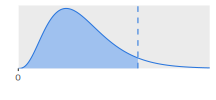
\includegraphics[width=.49\linewidth]{bookdownproj_files/figure-latex/unnamed-chunk-33-1} \end{center}

\begin{table}[!h]
\centering
\resizebox{\linewidth}{!}{
\begin{tabular}{>{}r|rrrrrrrrrrr}
\toprule
\multicolumn{1}{c}{ } & \multicolumn{11}{c}{Fläche} \\
\cmidrule(l{3pt}r{3pt}){2-12}
$df$ & 0,6 & 0,7 & 0,8 & 0,85 & 0,9 & 0,95 & 0,975 & 0,99 & 0,995 & 0,999 & 0,9995\\
\midrule
\cellcolor{gray!6}{1} & \cellcolor{gray!6}{0,708} & \cellcolor{gray!6}{1,074} & \cellcolor{gray!6}{1,642} & \cellcolor{gray!6}{2,072} & \cellcolor{gray!6}{2,706} & \cellcolor{gray!6}{3,841} & \cellcolor{gray!6}{5,024} & \cellcolor{gray!6}{6,635} & \cellcolor{gray!6}{7,879} & \cellcolor{gray!6}{10,828} & \cellcolor{gray!6}{12,116}\\
2 & 1,833 & 2,408 & 3,219 & 3,794 & 4,605 & 5,991 & 7,378 & 9,210 & 10,597 & 13,816 & 15,202\\
\cellcolor{gray!6}{3} & \cellcolor{gray!6}{2,946} & \cellcolor{gray!6}{3,665} & \cellcolor{gray!6}{4,642} & \cellcolor{gray!6}{5,317} & \cellcolor{gray!6}{6,251} & \cellcolor{gray!6}{7,815} & \cellcolor{gray!6}{9,348} & \cellcolor{gray!6}{11,345} & \cellcolor{gray!6}{12,838} & \cellcolor{gray!6}{16,266} & \cellcolor{gray!6}{17,730}\\
4 & 4,045 & 4,878 & 5,989 & 6,745 & 7,779 & 9,488 & 11,143 & 13,277 & 14,860 & 18,467 & 19,997\\
\cellcolor{gray!6}{5} & \cellcolor{gray!6}{5,132} & \cellcolor{gray!6}{6,064} & \cellcolor{gray!6}{7,289} & \cellcolor{gray!6}{8,115} & \cellcolor{gray!6}{9,236} & \cellcolor{gray!6}{11,070} & \cellcolor{gray!6}{12,833} & \cellcolor{gray!6}{15,086} & \cellcolor{gray!6}{16,750} & \cellcolor{gray!6}{20,515} & \cellcolor{gray!6}{22,105}\\
\addlinespace
6 & 6,211 & 7,231 & 8,558 & 9,446 & 10,645 & 12,592 & 14,449 & 16,812 & 18,548 & 22,458 & 24,103\\
\cellcolor{gray!6}{7} & \cellcolor{gray!6}{7,283} & \cellcolor{gray!6}{8,383} & \cellcolor{gray!6}{9,803} & \cellcolor{gray!6}{10,748} & \cellcolor{gray!6}{12,017} & \cellcolor{gray!6}{14,067} & \cellcolor{gray!6}{16,013} & \cellcolor{gray!6}{18,475} & \cellcolor{gray!6}{20,278} & \cellcolor{gray!6}{24,322} & \cellcolor{gray!6}{26,018}\\
8 & 8,351 & 9,524 & 11,030 & 12,027 & 13,362 & 15,507 & 17,535 & 20,090 & 21,955 & 26,124 & 27,868\\
\cellcolor{gray!6}{9} & \cellcolor{gray!6}{9,414} & \cellcolor{gray!6}{10,656} & \cellcolor{gray!6}{12,242} & \cellcolor{gray!6}{13,288} & \cellcolor{gray!6}{14,684} & \cellcolor{gray!6}{16,919} & \cellcolor{gray!6}{19,023} & \cellcolor{gray!6}{21,666} & \cellcolor{gray!6}{23,589} & \cellcolor{gray!6}{27,877} & \cellcolor{gray!6}{29,666}\\
10 & 10,473 & 11,781 & 13,442 & 14,534 & 15,987 & 18,307 & 20,483 & 23,209 & 25,188 & 29,588 & 31,420\\
\addlinespace
\cellcolor{gray!6}{11} & \cellcolor{gray!6}{11,530} & \cellcolor{gray!6}{12,899} & \cellcolor{gray!6}{14,631} & \cellcolor{gray!6}{15,767} & \cellcolor{gray!6}{17,275} & \cellcolor{gray!6}{19,675} & \cellcolor{gray!6}{21,920} & \cellcolor{gray!6}{24,725} & \cellcolor{gray!6}{26,757} & \cellcolor{gray!6}{31,264} & \cellcolor{gray!6}{33,137}\\
12 & 12,584 & 14,011 & 15,812 & 16,989 & 18,549 & 21,026 & 23,337 & 26,217 & 28,300 & 32,909 & 34,821\\
\cellcolor{gray!6}{13} & \cellcolor{gray!6}{13,636} & \cellcolor{gray!6}{15,119} & \cellcolor{gray!6}{16,985} & \cellcolor{gray!6}{18,202} & \cellcolor{gray!6}{19,812} & \cellcolor{gray!6}{22,362} & \cellcolor{gray!6}{24,736} & \cellcolor{gray!6}{27,688} & \cellcolor{gray!6}{29,819} & \cellcolor{gray!6}{34,528} & \cellcolor{gray!6}{36,478}\\
14 & 14,685 & 16,222 & 18,151 & 19,406 & 21,064 & 23,685 & 26,119 & 29,141 & 31,319 & 36,123 & 38,109\\
\cellcolor{gray!6}{15} & \cellcolor{gray!6}{15,733} & \cellcolor{gray!6}{17,322} & \cellcolor{gray!6}{19,311} & \cellcolor{gray!6}{20,603} & \cellcolor{gray!6}{22,307} & \cellcolor{gray!6}{24,996} & \cellcolor{gray!6}{27,488} & \cellcolor{gray!6}{30,578} & \cellcolor{gray!6}{32,801} & \cellcolor{gray!6}{37,697} & \cellcolor{gray!6}{39,719}\\
\addlinespace
16 & 16,780 & 18,418 & 20,465 & 21,793 & 23,542 & 26,296 & 28,845 & 32,000 & 34,267 & 39,252 & 41,308\\
\cellcolor{gray!6}{17} & \cellcolor{gray!6}{17,824} & \cellcolor{gray!6}{19,511} & \cellcolor{gray!6}{21,615} & \cellcolor{gray!6}{22,977} & \cellcolor{gray!6}{24,769} & \cellcolor{gray!6}{27,587} & \cellcolor{gray!6}{30,191} & \cellcolor{gray!6}{33,409} & \cellcolor{gray!6}{35,718} & \cellcolor{gray!6}{40,790} & \cellcolor{gray!6}{42,879}\\
18 & 18,868 & 20,601 & 22,760 & 24,155 & 25,989 & 28,869 & 31,526 & 34,805 & 37,156 & 42,312 & 44,434\\
\cellcolor{gray!6}{19} & \cellcolor{gray!6}{19,910} & \cellcolor{gray!6}{21,689} & \cellcolor{gray!6}{23,900} & \cellcolor{gray!6}{25,329} & \cellcolor{gray!6}{27,204} & \cellcolor{gray!6}{30,144} & \cellcolor{gray!6}{32,852} & \cellcolor{gray!6}{36,191} & \cellcolor{gray!6}{38,582} & \cellcolor{gray!6}{43,820} & \cellcolor{gray!6}{45,973}\\
20 & 20,951 & 22,775 & 25,038 & 26,498 & 28,412 & 31,410 & 34,170 & 37,566 & 39,997 & 45,315 & 47,498\\
\addlinespace
\cellcolor{gray!6}{25} & \cellcolor{gray!6}{26,143} & \cellcolor{gray!6}{28,172} & \cellcolor{gray!6}{30,675} & \cellcolor{gray!6}{32,282} & \cellcolor{gray!6}{34,382} & \cellcolor{gray!6}{37,652} & \cellcolor{gray!6}{40,646} & \cellcolor{gray!6}{44,314} & \cellcolor{gray!6}{46,928} & \cellcolor{gray!6}{52,620} & \cellcolor{gray!6}{54,947}\\
30 & 31,316 & 33,530 & 36,250 & 37,990 & 40,256 & 43,773 & 46,979 & 50,892 & 53,672 & 59,703 & 62,162\\
\cellcolor{gray!6}{35} & \cellcolor{gray!6}{36,475} & \cellcolor{gray!6}{38,859} & \cellcolor{gray!6}{41,778} & \cellcolor{gray!6}{43,640} & \cellcolor{gray!6}{46,059} & \cellcolor{gray!6}{49,802} & \cellcolor{gray!6}{53,203} & \cellcolor{gray!6}{57,342} & \cellcolor{gray!6}{60,275} & \cellcolor{gray!6}{66,619} & \cellcolor{gray!6}{69,199}\\
40 & 41,622 & 44,165 & 47,269 & 49,244 & 51,805 & 55,758 & 59,342 & 63,691 & 66,766 & 73,402 & 76,095\\
\cellcolor{gray!6}{45} & \cellcolor{gray!6}{46,761} & \cellcolor{gray!6}{49,452} & \cellcolor{gray!6}{52,729} & \cellcolor{gray!6}{54,810} & \cellcolor{gray!6}{57,505} & \cellcolor{gray!6}{61,656} & \cellcolor{gray!6}{65,410} & \cellcolor{gray!6}{69,957} & \cellcolor{gray!6}{73,166} & \cellcolor{gray!6}{80,077} & \cellcolor{gray!6}{82,876}\\
\addlinespace
50 & 51,892 & 54,723 & 58,164 & 60,346 & 63,167 & 67,505 & 71,420 & 76,154 & 79,490 & 86,661 & 89,561\\
\cellcolor{gray!6}{60} & \cellcolor{gray!6}{62,135} & \cellcolor{gray!6}{65,227} & \cellcolor{gray!6}{68,972} & \cellcolor{gray!6}{71,341} & \cellcolor{gray!6}{74,397} & \cellcolor{gray!6}{79,082} & \cellcolor{gray!6}{83,298} & \cellcolor{gray!6}{88,379} & \cellcolor{gray!6}{91,952} & \cellcolor{gray!6}{99,607} & \cellcolor{gray!6}{102,695}\\
70 & 72,358 & 75,689 & 79,715 & 82,255 & 85,527 & 90,531 & 95,023 & 100,425 & 104,215 & 112,317 & 115,578\\
\cellcolor{gray!6}{80} & \cellcolor{gray!6}{82,566} & \cellcolor{gray!6}{86,120} & \cellcolor{gray!6}{90,405} & \cellcolor{gray!6}{93,106} & \cellcolor{gray!6}{96,578} & \cellcolor{gray!6}{101,879} & \cellcolor{gray!6}{106,629} & \cellcolor{gray!6}{112,329} & \cellcolor{gray!6}{116,321} & \cellcolor{gray!6}{124,839} & \cellcolor{gray!6}{128,261}\\
90 & 92,761 & 96,524 & 101,054 & 103,904 & 107,565 & 113,145 & 118,136 & 124,116 & 128,299 & 137,208 & 140,782\\
\addlinespace
\cellcolor{gray!6}{100} & \cellcolor{gray!6}{102,946} & \cellcolor{gray!6}{106,906} & \cellcolor{gray!6}{111,667} & \cellcolor{gray!6}{114,659} & \cellcolor{gray!6}{118,498} & \cellcolor{gray!6}{124,342} & \cellcolor{gray!6}{129,561} & \cellcolor{gray!6}{135,807} & \cellcolor{gray!6}{140,169} & \cellcolor{gray!6}{149,449} & \cellcolor{gray!6}{153,167}\\
110 & 113,121 & 117,269 & 122,250 & 125,376 & 129,385 & 135,480 & 140,917 & 147,414 & 151,948 & 161,581 & 165,435\\
\cellcolor{gray!6}{120} & \cellcolor{gray!6}{123,289} & \cellcolor{gray!6}{127,616} & \cellcolor{gray!6}{132,806} & \cellcolor{gray!6}{136,062} & \cellcolor{gray!6}{140,233} & \cellcolor{gray!6}{146,567} & \cellcolor{gray!6}{152,211} & \cellcolor{gray!6}{158,950} & \cellcolor{gray!6}{163,648} & \cellcolor{gray!6}{173,617} & \cellcolor{gray!6}{177,603}\\
130 & 133,450 & 137,949 & 143,340 & 146,719 & 151,045 & 157,610 & 163,453 & 170,423 & 175,278 & 185,571 & 189,682\\
\cellcolor{gray!6}{140} & \cellcolor{gray!6}{143,604} & \cellcolor{gray!6}{148,269} & \cellcolor{gray!6}{153,854} & \cellcolor{gray!6}{157,352} & \cellcolor{gray!6}{161,827} & \cellcolor{gray!6}{168,613} & \cellcolor{gray!6}{174,648} & \cellcolor{gray!6}{181,840} & \cellcolor{gray!6}{186,847} & \cellcolor{gray!6}{197,451} & \cellcolor{gray!6}{201,683}\\
\addlinespace
150 & 153,753 & 158,577 & 164,349 & 167,962 & 172,581 & 179,581 & 185,800 & 193,208 & 198,360 & 209,265 & 213,613\\
\cellcolor{gray!6}{200} & \cellcolor{gray!6}{204,434} & \cellcolor{gray!6}{209,985} & \cellcolor{gray!6}{216,609} & \cellcolor{gray!6}{220,744} & \cellcolor{gray!6}{226,021} & \cellcolor{gray!6}{233,994} & \cellcolor{gray!6}{241,058} & \cellcolor{gray!6}{249,445} & \cellcolor{gray!6}{255,264} & \cellcolor{gray!6}{267,541} & \cellcolor{gray!6}{272,423}\\
300 & 305,574 & 312,346 & 320,397 & 325,409 & 331,789 & 341,395 & 349,874 & 359,906 & 366,844 & 381,425 & 387,203\\
\cellcolor{gray!6}{400} & \cellcolor{gray!6}{406,535} & \cellcolor{gray!6}{414,335} & \cellcolor{gray!6}{423,590} & \cellcolor{gray!6}{429,340} & \cellcolor{gray!6}{436,649} & \cellcolor{gray!6}{447,632} & \cellcolor{gray!6}{457,305} & \cellcolor{gray!6}{468,724} & \cellcolor{gray!6}{476,606} & \cellcolor{gray!6}{493,132} & \cellcolor{gray!6}{499,666}\\
500 & 507,382 & 516,087 & 526,401 & 532,803 & 540,930 & 553,127 & 563,852 & 576,493 & 585,207 & 603,446 & 610,648\\
\bottomrule
\end{tabular}}
\end{table}

\pagebreak

\hypertarget{quellen-9}{%
\subsection{Quellen}\label{quellen-9}}

\hypertarget{refs}{}
\begin{CSLReferences}{1}{0}
\leavevmode\hypertarget{ref-bahrenberg}{}%
Bahrenberg, Gerhard, Ernst Giese und Josef Nipper. 2010. \emph{Statistische Methoden in der Geographie}. Bd. 1. Univariate und bivariate Statistik. Stuttgart: Bornträger.

\leavevmode\hypertarget{ref-benninghaus}{}%
Benninghaus, Hans. 2007. \emph{Deskriptive Statistik. Eine Einführung für Sozialwissenschaftler}. Wiesbaden: VS Verlag.

\leavevmode\hypertarget{ref-bortz}{}%
Bortz, Jürgen und Christof Schuster. 2010. \emph{Statistik für Human- und Sozialwissenschaftler}. Berlin: Springer.

\leavevmode\hypertarget{ref-haseloff}{}%
Haseloff, Otto W., Hans-Joachim Hoffmann, John H Maindonald und W John Braun. 1968. \emph{Kleines Lehrbuch der Statistik DAAG. Data Analysis and Graphics Data and Functions}. Berlin: de Gruyter.

\leavevmode\hypertarget{ref-klemm}{}%
Klemm, Elmar. 2002. \emph{Einführung in die Statistik. Für die Sozialwissenschaften}. Wiesbaden: Westdeutscher Verlag.

\leavevmode\hypertarget{ref-r}{}%
R Core Team. 2018. R: A Language and Environment for Statistical Computing. Wien: R Foundation for Statistical Computing. \url{https://www.R-project.org/} (zugegriffen: ).

\end{CSLReferences}

\end{document}
